\documentclass[titlepage, 12pt]{report}

\usepackage[utf8]{inputenc}
\usepackage[T1]{fontenc}
\usepackage[francais]{babel}
\usepackage{listings} %listings for code
\usepackage{graphicx} % can modify title style
\usepackage{titling} % can use pretitle to have a picture on title page
\usepackage{chngcntr} % permits to reset chapter numerization in each part
\usepackage{hyperref} % makes table of contents and list of figures clickable 
\usepackage{makecell} % can create newline in a table cell easily
\usepackage{scrextend}
\usepackage{enumitem}
\usepackage{tabularx}


%\hypersetup{colorlinks,citecolor=black,filecolor=black,linkcolor=black,urlcolor=black}

\counterwithin*{chapter}{part}

\addtolength{\oddsidemargin}{-2cm}
\addtolength{\evensidemargin}{-2cm}
\addtolength{\textwidth}{4cm}
\addtolength{\topmargin}{-2cm}
\addtolength{\textheight}{4cm}

\setcounter{secnumdepth}{3}

% Title Page

\pretitle{
	\begin{center}
		\LARGE
		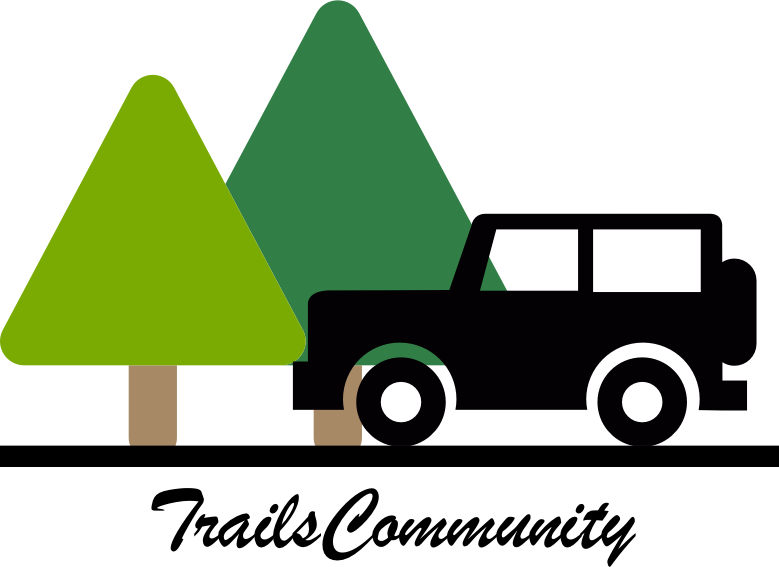
\includegraphics[width=\textwidth]{Images/TrailsCommunity_doc.png}\\[\bigskipamount]
	}
	
	\posttitle{\end{center}}

		\title{Rapport de projet - Assitant Offroad}
		
		\author{BELLANGER Stéphen \and
			MONNIER Ysée \and
			DESHORS Yann}
		\date{Novembre 2016 - Decembre 2016}
		


\begin{document}
	
\maketitle

\tableofcontents

\listoffigures 

\part{Spécification des exigences logicielles}

\chapter{Introduction}

Cette section fournit  une vue d'ensemble de tout ce qui est inclus dans ce document SRS. De plus, l'objectif de ce document est détaillé et une liste de définitions est fournie.

\section{Objectifs}

L'objectif de ce document est de fournir une description détaillée des conditions requises pour l'application mobile TrailsCommunity.
Il illustrera le but et la description complète du développement du système.
Il expliquera également les contraintes du système, l'interface et les interactions avec les applications externes. Ce document est principalement destiné à être proposé à un client pour son approbation. C'est aussi une référence pour le développement de la première version du système pour l'équipe de développement.

\section{Portée}

TrailsCommunity est une application mobile GPS qui permet aux utilisateurs de connaitre en temps réel le positionnement des autres participants d'une activité en pleine air. L'ensemble des activités sont regroupés en type qui seront limités à une liste pré-défini.
L'application doit être gratuite, simple d'utilisation et ergonomique.
L'organisateur de l'activité devra fournir deux adresses. Une pour le point de départ de l'application et la deuxième pour le point d'arrivé. La création des sessions se fera directement sur l'application mobile.
En outre, le logiciel a besoin à la fois d'Internet et d'une connexion GPS pour récupérer et afficher les résultats. Tous les systèmes d'informations sont conservés dans une base de données, qui se trouve sur un serveur web. De plus une base de données interne sera créer pour pouvoir stocker différentes données relatives aux sessions lorsque l'utilisateur utilise l'application en hors-ligne.
Le logiciel interagit également avec l'API Google Maps qui permettra d'afficher et de tracer les différents parcours des utilisateurs. De plus, le téléphone doit aussi être composé d'un GPS pour pouvoir localiser l'utilisateur à tout moment. 
L'application a également la capacité de représenter à la fois des informations sommaires et détaillées des différentes statistiques de l'utilisateur courant mais aussi des autres participants de la session en cours.

\section{Définitions}
\begin{labeling}{alligator}
	\item [session] : une session est une activité disponible dans l’application.
	\item [visiteur] : personne n’étant pas identifiée.
	\item [utilisateur] : personne identifiée à l’application. Il possède les choix de créer ou de rejoindre une session.
	\item [organisateur] : utilisateur ayant créé une session et pouvant la gérer.
	\item [participant] : utilisateur qui a rejoint une session.
	\item [waypoint] : désigne un point de la route a atteindre où doit avoir lieu un changement de cap.
\end{labeling}


\section{Références}
\begin{labeling}{alligator}
	\item [The Institute of Electrical and Electronic Engineer NY USA] IEEE Recommented Practice for SRS, \url{http://www.utdallas.edu/~chung/RE/IEEE830-1993.pdf}
	\item [Chalmers] IEEE standards - SRS Example, 2010, \url{http://www.cse.chalmers.se/~feldt/courses/reqeng/examples/srs_example_2010_group2.pdf}
	\item [Droid5 Informatics Pvt Ltd] androidhive, 2016, \url{http://www.androidhive.info}
	\item [Oracle] Java 8 Documentation, 2016, \url{https://docs.oracle.com/javase/8/docs/api/}
	\item [Google] Android Documentation, 2016, \url{https://developer.android.com/guide}
	\item [James Britt] Ruby Doc, 2016, \url{http://ruby-doc.org}
	\item [Rails Community] Ruby On Rails Documentation, 2016, \url{http://rubyonrails.org}
\end{labeling}

\section{Aperçu}

\paragraph{}Différentes techniques de spécification sont utilisées afin de préciser les exigences plus précisément pour différents publics. Cependant, le lecteur principal sera le correcteur du projet.

\paragraph{}Le reste de ce document comprend cinq chapitres. Le second fournit une vue d'ensemble de la fonctionnalité du système et de l'interaction de l'application avec d'autres systèmes. En outre, le chapitre mentionne également les contraintes du systèmes et les hypothèses sur le produit.
Le troisième chapitre fournit la conception et l'ergonomie de l'application.
Le quatrième chapitre concerne l'ensemble des exigences fonctionnelles de l'application. Elle sont triés en différentes parties.
Le cinquième chapitre regroupe un ensemble de diagrammes UML qui sont primordiales pour la compréhension mais aussi pour le développement de l'application.

\section{Outils utilisés}

\paragraph{}De nombreux outils seront utilisés tout au long du développement de l'application. En effet, l'équipe utilisera le logiciel TRELLO pour la gestion de projet et la répartition des tâches entre les différents membres. Dans un domaine plus précis, les développeurs ont mis en place un dépôt GIT qui permet de pouvoir centraliser l'ensemble du travail réalisé ainsi que de gérer les différentes version du produit. De plus, un outil d'intégration continue à été intégré pour suivre à chaque dépôt de code, la qualité de celui-ci.

\chapter{Description générale}

\section{Perspective du produit}

\paragraph{}Ce système se compose de deux parties : une application mobile et un serveur web.
L'application Android sera utilisé pour la gestion des sessions. Elle permettra d'afficher en fonction d'une session sélectionner, sur une carte Google maps les différentes positions des participants.
\paragraph{}Le serveur sera tant qu'à lui capable de gérer la récolte et la gestion des données envoyer par l'application.
De plus, un mode hors-ligne sera disponible sur l'application. En effet, elle basculera sur une base de données interne qui stockera l'ensemble des données. Lorsque l'utilisateur se reconnectera à internet. L'ensemble des informations stockées en interne seront envoyé au serveur.
\paragraph{}L'application mobile devra communiquer avec un GPS qui se situe au sein du mobile. Le GPS fournira les emplacements de l'utilisateur. Pour ce qui est des autres participants, leurs coordonnées seront stockées dans la base de données du serveur. De plus, des statistiques sur l'utilisateur courant ainsi qu'un chat seront disponible pour permettre au différents membres de pouvoir communiquer ensemble.
\paragraph{}De manière transparente comme il s'agit d'un produit axé sur la récolte de données, il lui faudra une base de données. La communication avec la base de données se passera via internet. Cependant, comme expliqué précédemment, l'application possèdera une base de données interne pour gérer le mode hors-ligne. 

\section{Fonctions du produit}

\paragraph{}Avec l'application mobile, les utilisateurs pourront créer un compte utilisateur. Cette première étape va permettre de collecter différentes informations primordiales sur les utilisateurs. 

\paragraph{}Après la réalisation de cette première étape, et la connexion de ceux-ci, les utilisateurs pourront sélectionner des sessions. Le résultat sera basé sur les sessions que l'utilisateur sélectionne. Il existe 3 types de sessions. Les sessions actives, elle sont encore réalisable et ne sont pas encore clôturées. Cela veut donc dire que leurs dates de fin ne sont pas dépassées. Dans ces sessions, un chat en temps réel est disponible permettant de communiquer avec tout les participants.
\paragraph{}Les sessions clôturé dont l'utilisateur à participé. Elle se classe dans la section historique ce qui permet à l'utilisateur courant de pouvoir revisualiser ses anciennes statistiques.
\paragraph{}Enfin les sessions dont l'utilisateur est le créateur. Il a donc les droits de modifications sur celle-ci.

\paragraph{}L'application va permet après sélection d'une session, d'afficher une carte Google maps ainsi qu'un ensemble de points permettant de décrire le déplacement des différents utilisateurs actif de la session.
De plus, les sessions pourront être directement créée depuis l'application.

\section{Caractéristique de l'utilisateur}

\paragraph{}Il existe quartes types d'acteurs qui interagissent avec le système : le visiteur, l'utilisateur, le participant et l'organisateur. Chacun de ces quartes a une utilisation différente du système affin que chacun aient leurs propres exigences.

\paragraph{}Les visiteurs de l'application mobile ne peuvent utiliser TrailsCommunity si il ne sont pas connecter. Cela signifie que le visiteur doit être en mesure de pouvoir créer un compte utilisateur et ainsi de pouvoir se connecter.

\paragraph{}Les visiteurs connectés peuvent alors visualiser l'ensemble des sessions actives mais aussi leur historique de session ainsi que les sessions dont ils sont organisateurs.
De plus, ils peuvent modifier leurs coordonnées personnelles.

\paragraph{}Les participants sont des acteurs qui ont rejoint une session active, ils peuvent alors ajouter un waypoint et le partager à l'ensemble des participants. Ils peuvent aussi communiquer via un chat en temps réel. De plus, ils peuvent consulter leurs statistiques en cours.

\paragraph{}Enfin, les organisateurs sont des utilisateurs qui ont créée une nouvelle session. En effet, ce sont eux dont l'impulsion est venu pour organiser une activité. Il vont pouvoir partager le mot de passe de la session pour pouvoir la rejoindre.

\section{Contraintes}

\paragraph{}L'application mobile est limitée au système de navigation GPS du téléphone portable. Comme il existe plusieurs système de fabricants de GPS, la précision n'est pas la même pour chacun d'entre eux. En outre, il peut y avoir une différences de navigation en fonction des téléphones.

\paragraph{}La connexion internet est également une contrainte pour l'application. Puisqu'elle récupère les données de la base de données, il est crucial qu'il existe une connexion. De plus, en fonction du réseau, il est possible d'avoir une différence du temps de réception des données plus lente.
Il existera des fonctionnalités hors-ligne qui permettra entre autre de pouvoir basculer sur un nouveau protocole pour que les utilisateurs puissent continuer à communiquer entre eux sur le chat : le protocole SMS. L'ensemble des données des sessions récoltés sont alors stockées dans une base de données interne du mobile. Lors de la récupération du réseau internet, l'application va alors recevoir l'ensemble des données collectés en dur et va reprendre son état d'envoi naturel.

\section{Hypothèses et dépendances}

\paragraph{}Le produit sera toujours utilisé sur les téléphones mobiles Android qui ont assez de performances. Si le téléphone ne dispose pas de ressources matérielles suffisantes pour l'application. Elle peut ne pas fonctionner comme prévu ou même pas du tout.
De plus, la version minimum d'Android doit être Jelly Belly (Version 16). 

\paragraph{}Une autre hypothèse est que les composants GPS de tous les téléphones fonctionnent de la même manière. Si les téléphone on un système GPS est différent des normes, l'application doit être spécifiquement adaptée à chaque interface.

\section{Répartition des besoins}

\paragraph{}Dans le cas où le projet est retardé, certaines exigences pourraient être transférées au prochaine version de l'application. Les exigences avec une priorités haute doivent être développé lors du rendu de la première version de l'application.

\chapter{Exigences particulières}

\paragraph{}Cette section contient toutes les exigences fonctionnelles et de qualité du système. Il donne une description du système et de toutes ses caractéristiques.

\section{Exigences externe de l'interface}

\paragraph{}Cette section fournit une description détaillée de toutes les entrées et sorties du système. Il donne également une description des interfaces homme-machine et fournit des prototypes de base de l'interface pour l'utilisateur.

\section{Les interfaces utilisateurs}

\paragraph{}Un visiteur de l'application mobile devrait voir la page d'ouverture de session quand il ouvre l'application. Pour la connexion au compte utilisateur, il lui est absolument nécessaire de posséder un compte utilisateur composé d'une adresse mail et du mot de passe associé.

\begin{figure}[!h]
	\caption{Maquette de l'IHM pour la connexion}
	\label{login}
	\centering
	\includegraphics[scale=0.2]{images/mockups/login.png}
\end{figure}

\clearpage

\paragraph{}Pour la création d'un compte utilisateur, il est nécessaire de remplir l'ensemble des champs de l'interface. Toutefois, il sera possible de modifier son pseudonyme ainsi que son numéro de téléphone plus tard après sa connexion.

\begin{figure}[!h]
	\caption{Maquette de l'IHM pour la création d'un compte utilisateur}
	\label{create_user_account}
	\centering
	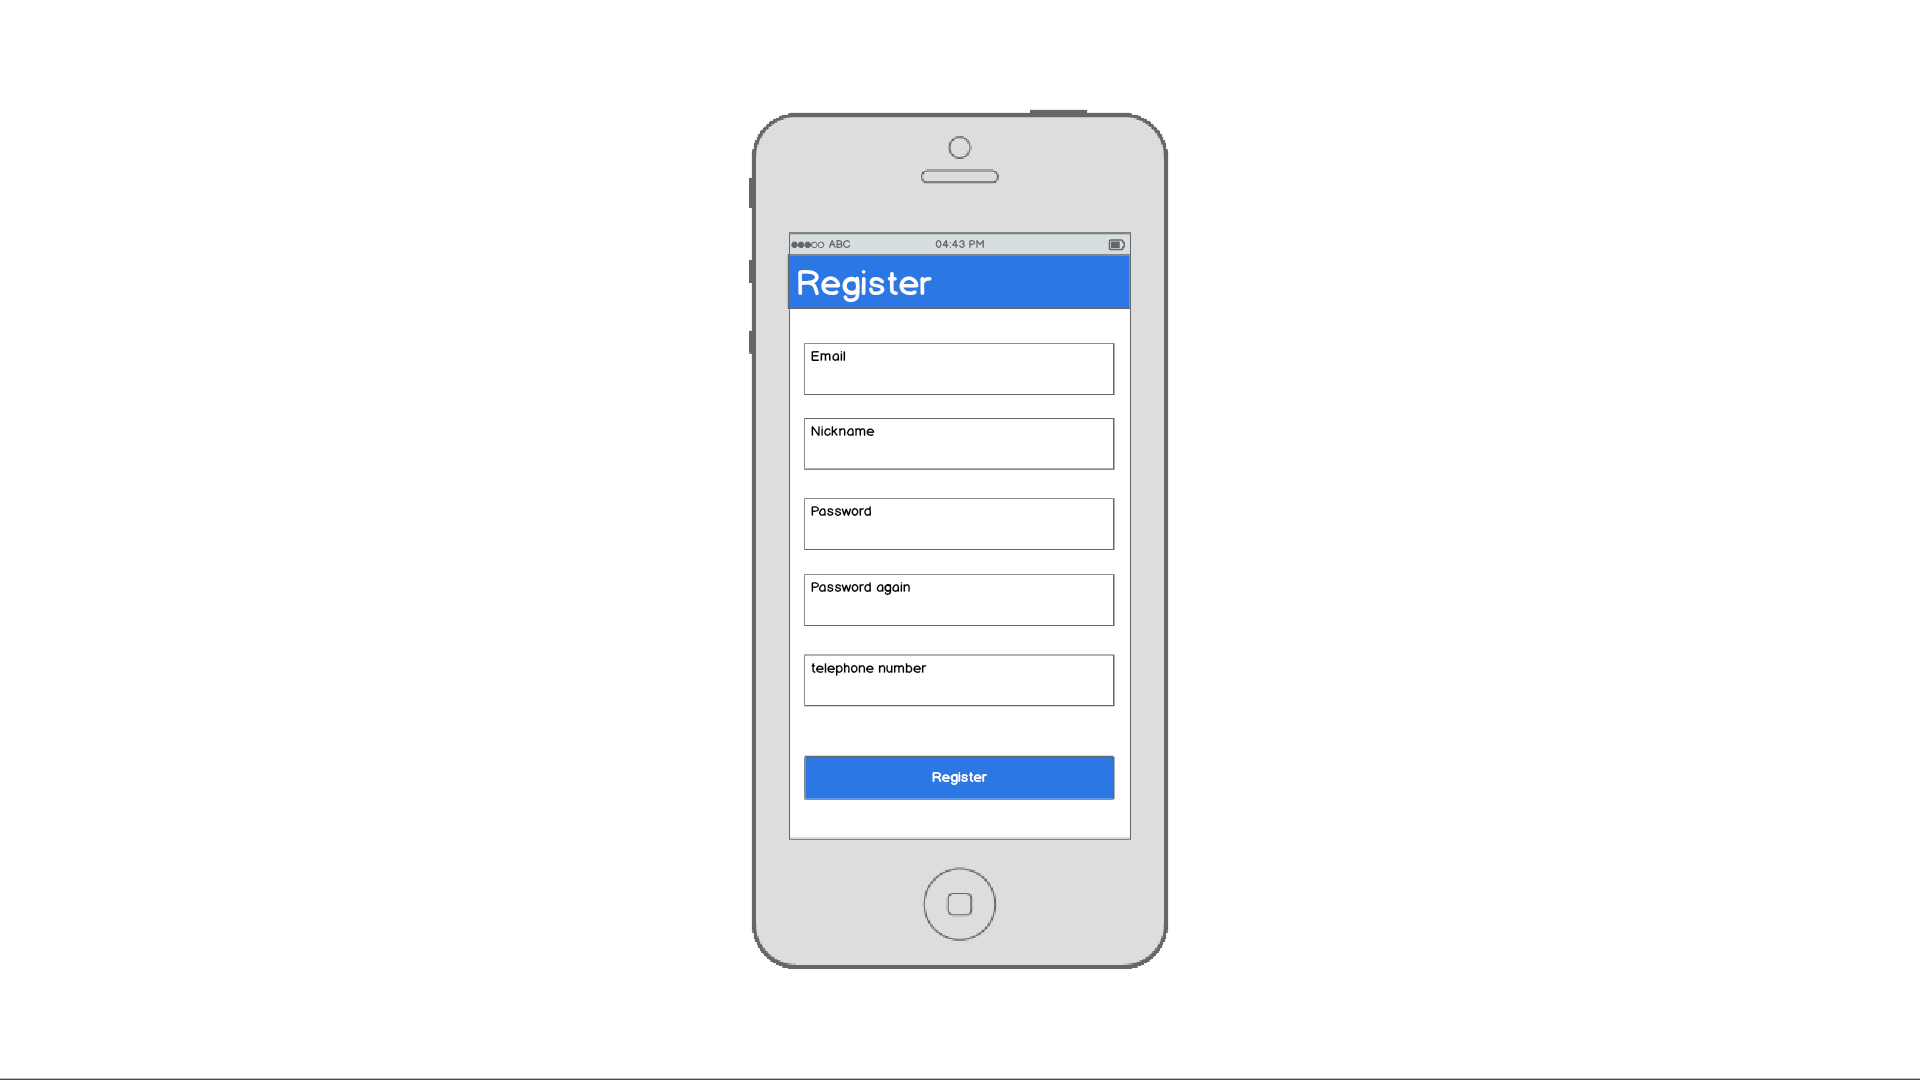
\includegraphics[scale=0.3]{images/mockups/register.png}
\end{figure}

\clearpage

\paragraph{}Après la connexion à un compte utilisateur, celui-ci peut alors choisir entre des sessions actives, les sessions dont il est l'organisateur ou des sessions clôturer qui sont dans la liste des historiques. L'icône plus permet de créer une nouvelle session. De plus, les boutons avec les 3 points permettent d'afficher une liste déroulante des différentes actions disponible sur cette interface. Les actions disponibles sont : la modification de ses données utilisateurs ainsi que la déconnexion.

\begin{figure}[!h]
	\caption{Maquette de l'IHM pour l'affichage des différentes sessions}
	\label{all_sessions}
	\centering
	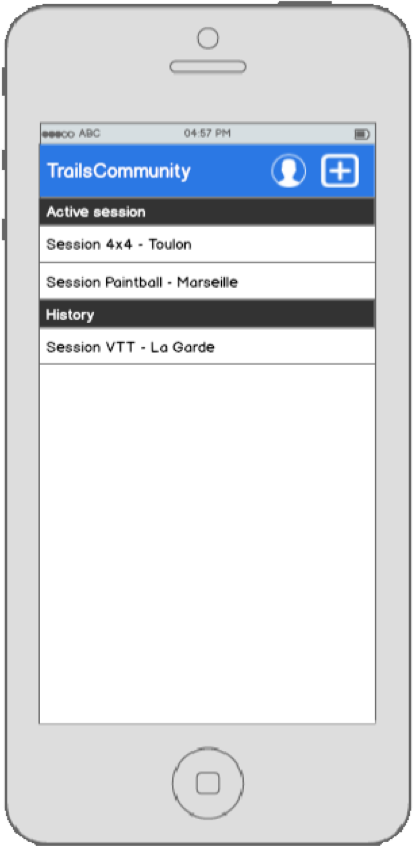
\includegraphics[scale=0.3]{images/mockups/session_view.png}
\end{figure}

\clearpage

\paragraph{}Pour la modification des données utilisateurs, seulement le pseudonyme et le numéro de téléphone peuvent être modifié.

\begin{figure}[!h]
	\caption{Maquette de l'IHM pour la modification des données utilisateurs}
	\label{modify_user_account}
	\centering
	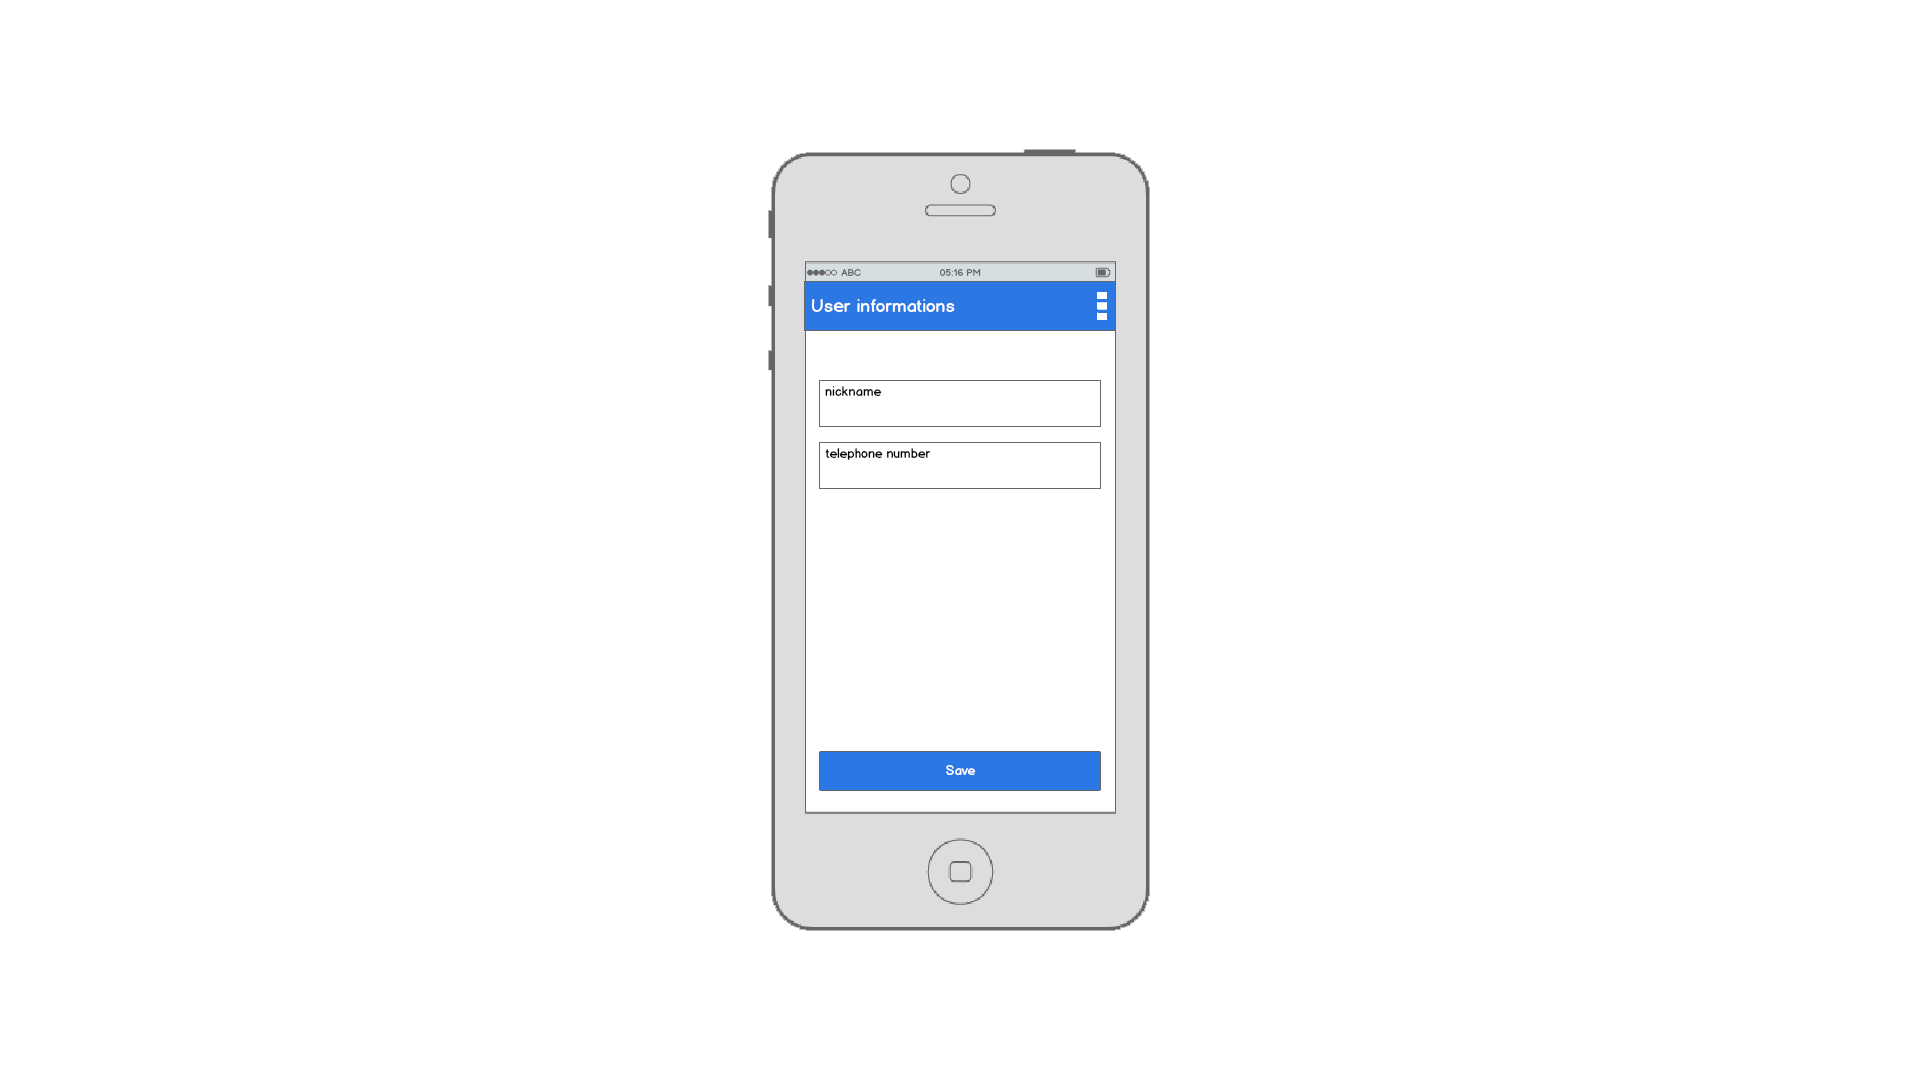
\includegraphics[scale=0.3]{images/mockups/modify_user_profile.png}
\end{figure}

\clearpage

\paragraph{}La création d'une session possède de nombreux champs texte obligatoire. Les adresses des lieux de départ et d'arrivé seront directement convertis en données GPS. De plus, lors du clique sur le champ texte de la date de départ, ue boite de dialogue apparaitra avec un calendrier spécifique à Android. A noter que le champ du mot de passe ne sera connu que par l'organisateur de la session.

\begin{figure}[!h]
	\caption{Maquette de l'IHM pour la création d'une session}
	\label{create_session}
	\centering
	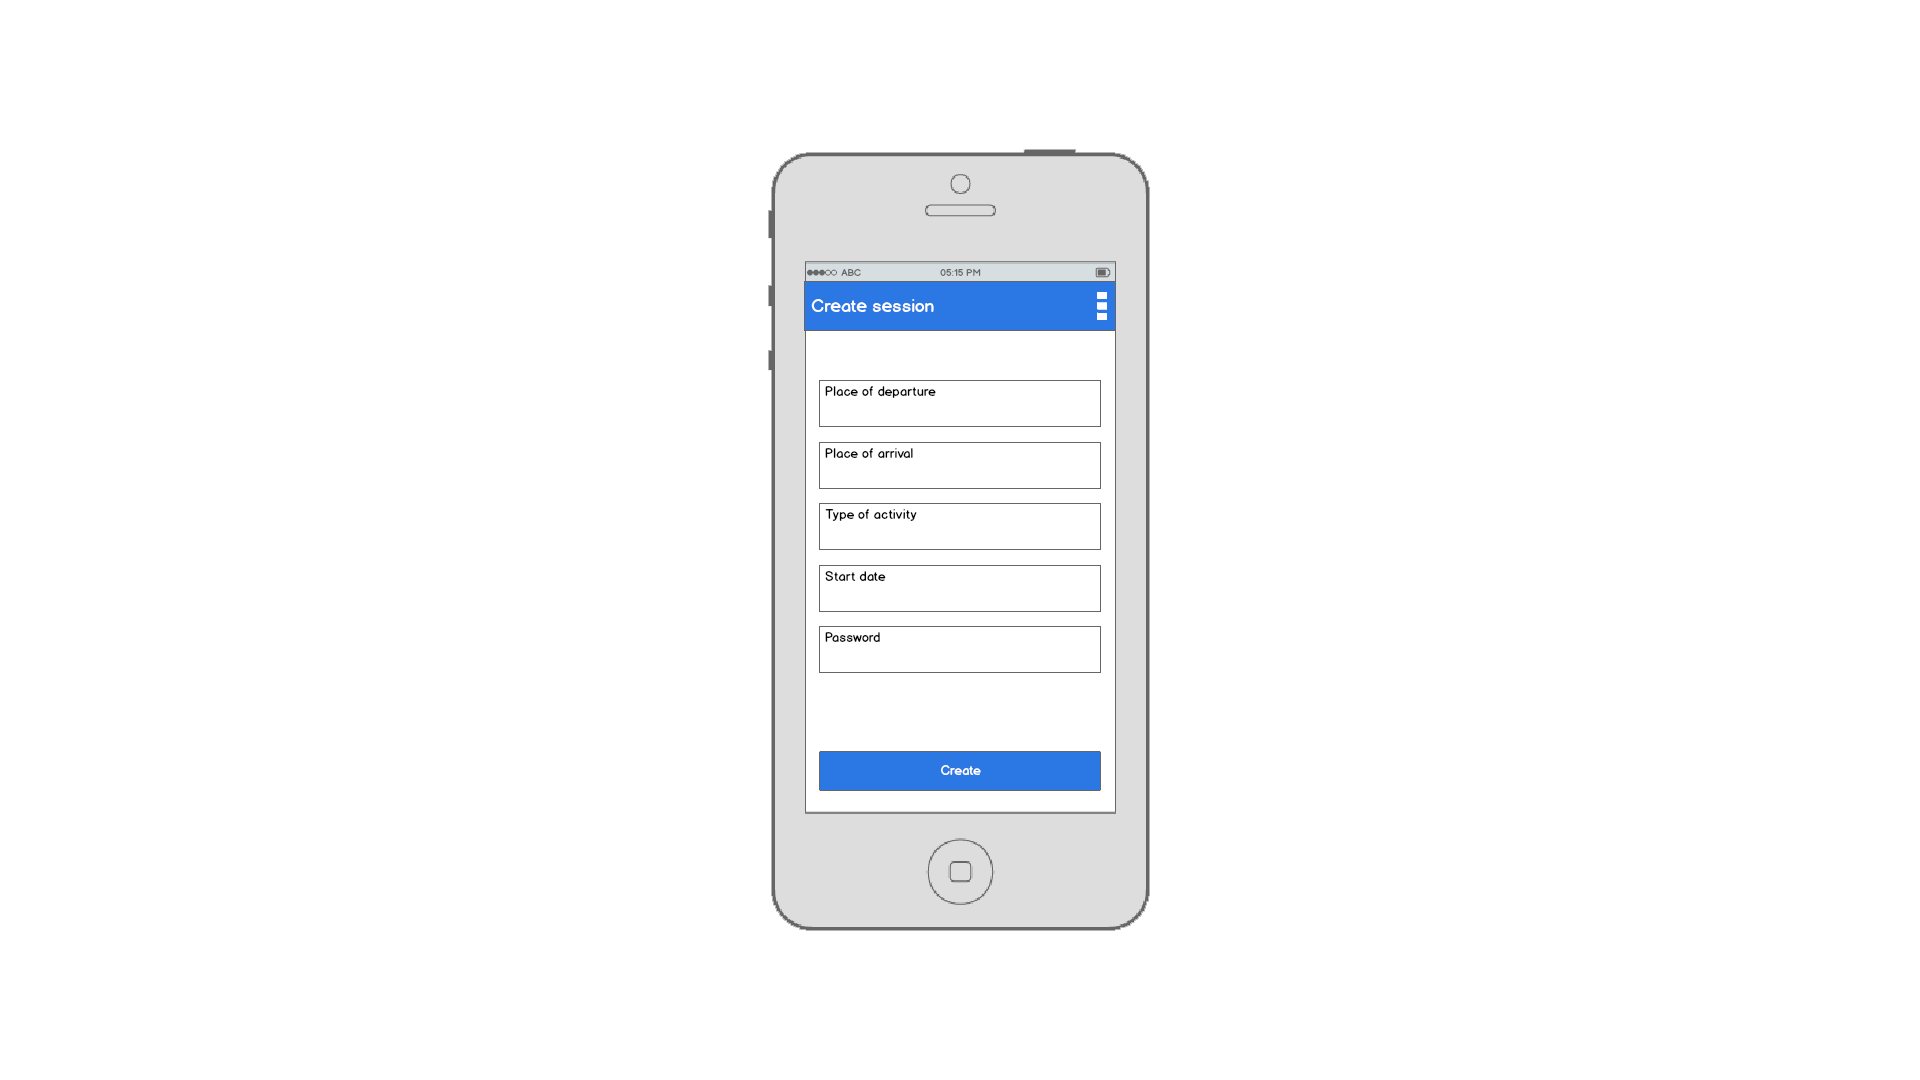
\includegraphics[scale=0.3]{images/mockups/create_session.png}
\end{figure}

\clearpage

\paragraph{}Lorsque l'utilisateur ouvre une session qui est dans sa liste de session historique. Cette interface apparait avec des actions propres au session historique.

\begin{figure}[!h]
	\caption{Maquette de l'IHM pour l'affichage d'une session historique}
	\label{history_session}
	\centering
	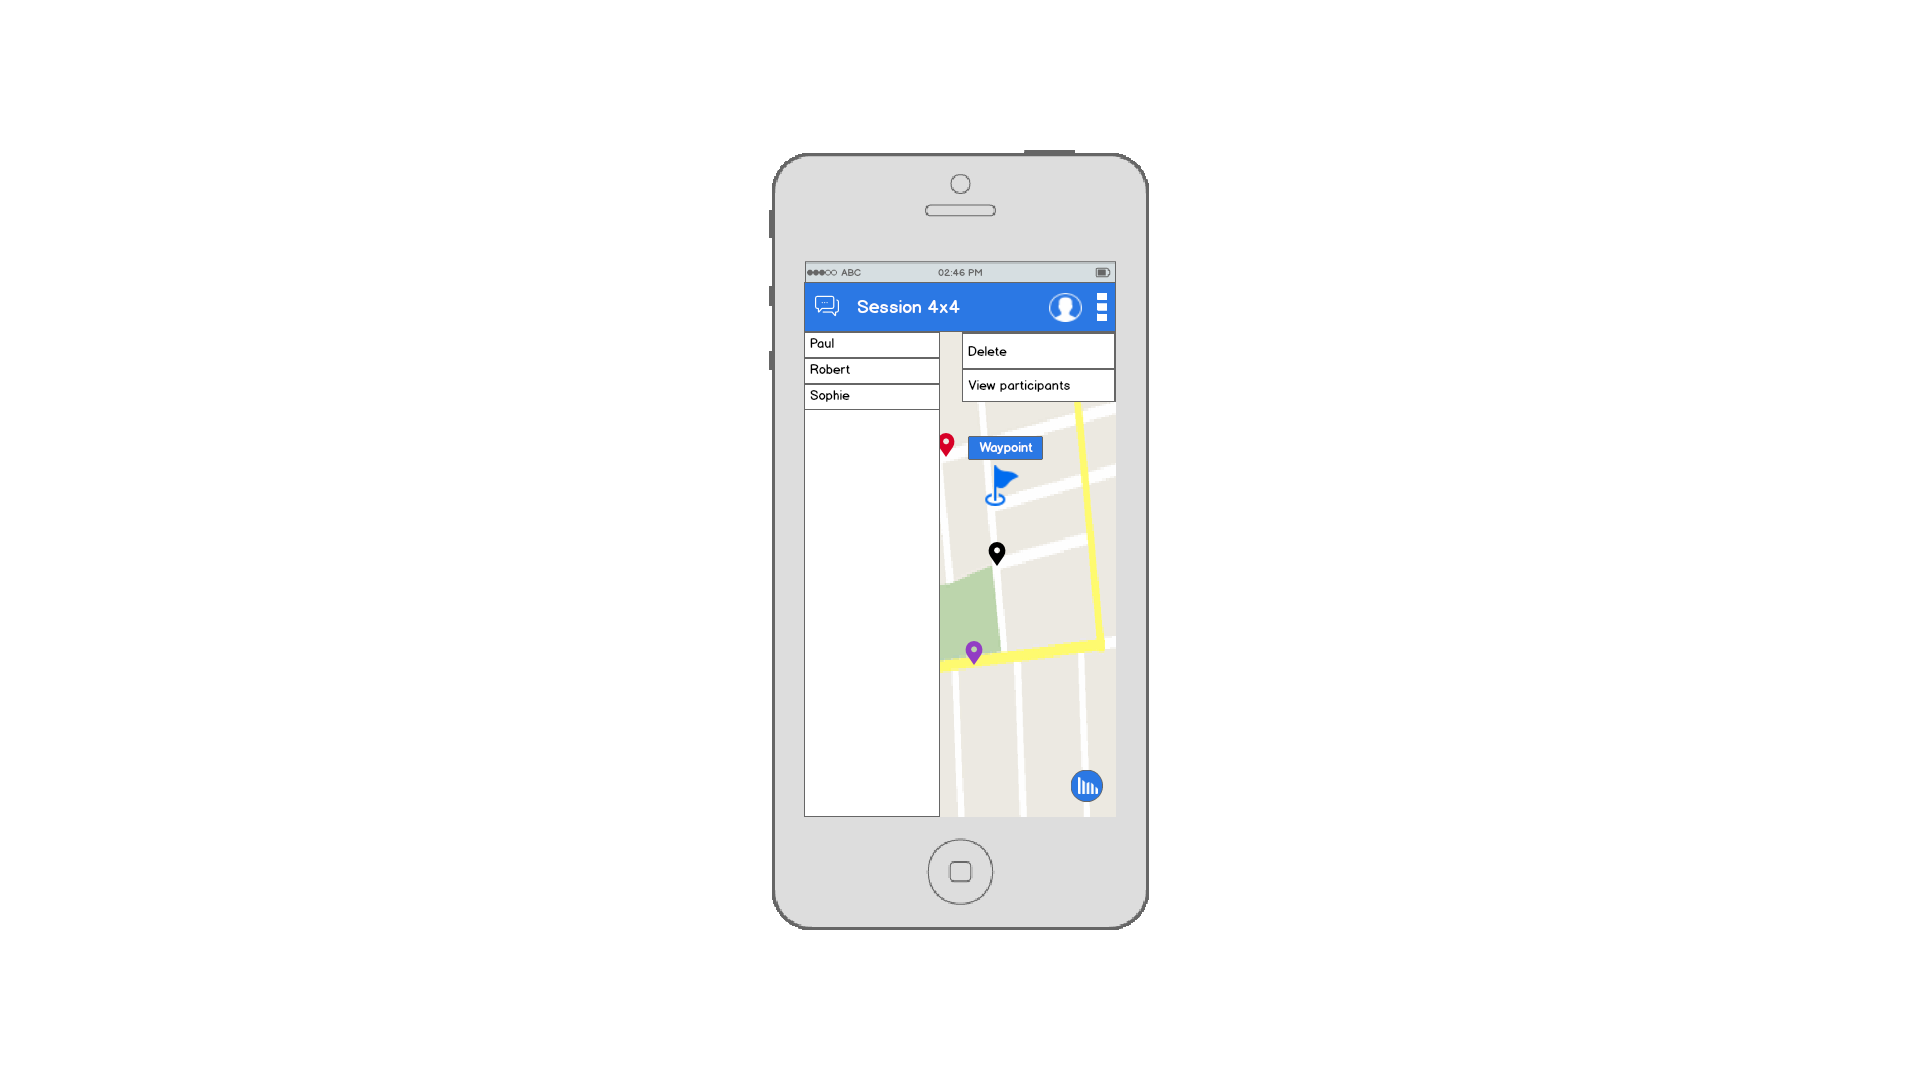
\includegraphics[scale=0.3]{images/mockups/history_session.png}
\end{figure}

\clearpage

\paragraph{}Cette maquette montre l'interface d'une session complètement vide. Seulement la Google maps y apparait. Lorsque l'utilisateur a choisit une session dont il est l'organisateur, une action est disponible lorsque celui-ci clique sur les trois petits points : clôturer la session. Une popup de confirmation va alors apparaitre pour qu'il puisse confirmer son action.

\begin{figure}[!h]
	\caption{Maquette de l'IHM pour l'affichage du Google map vide}
	\label{google_map_view}
	\centering
	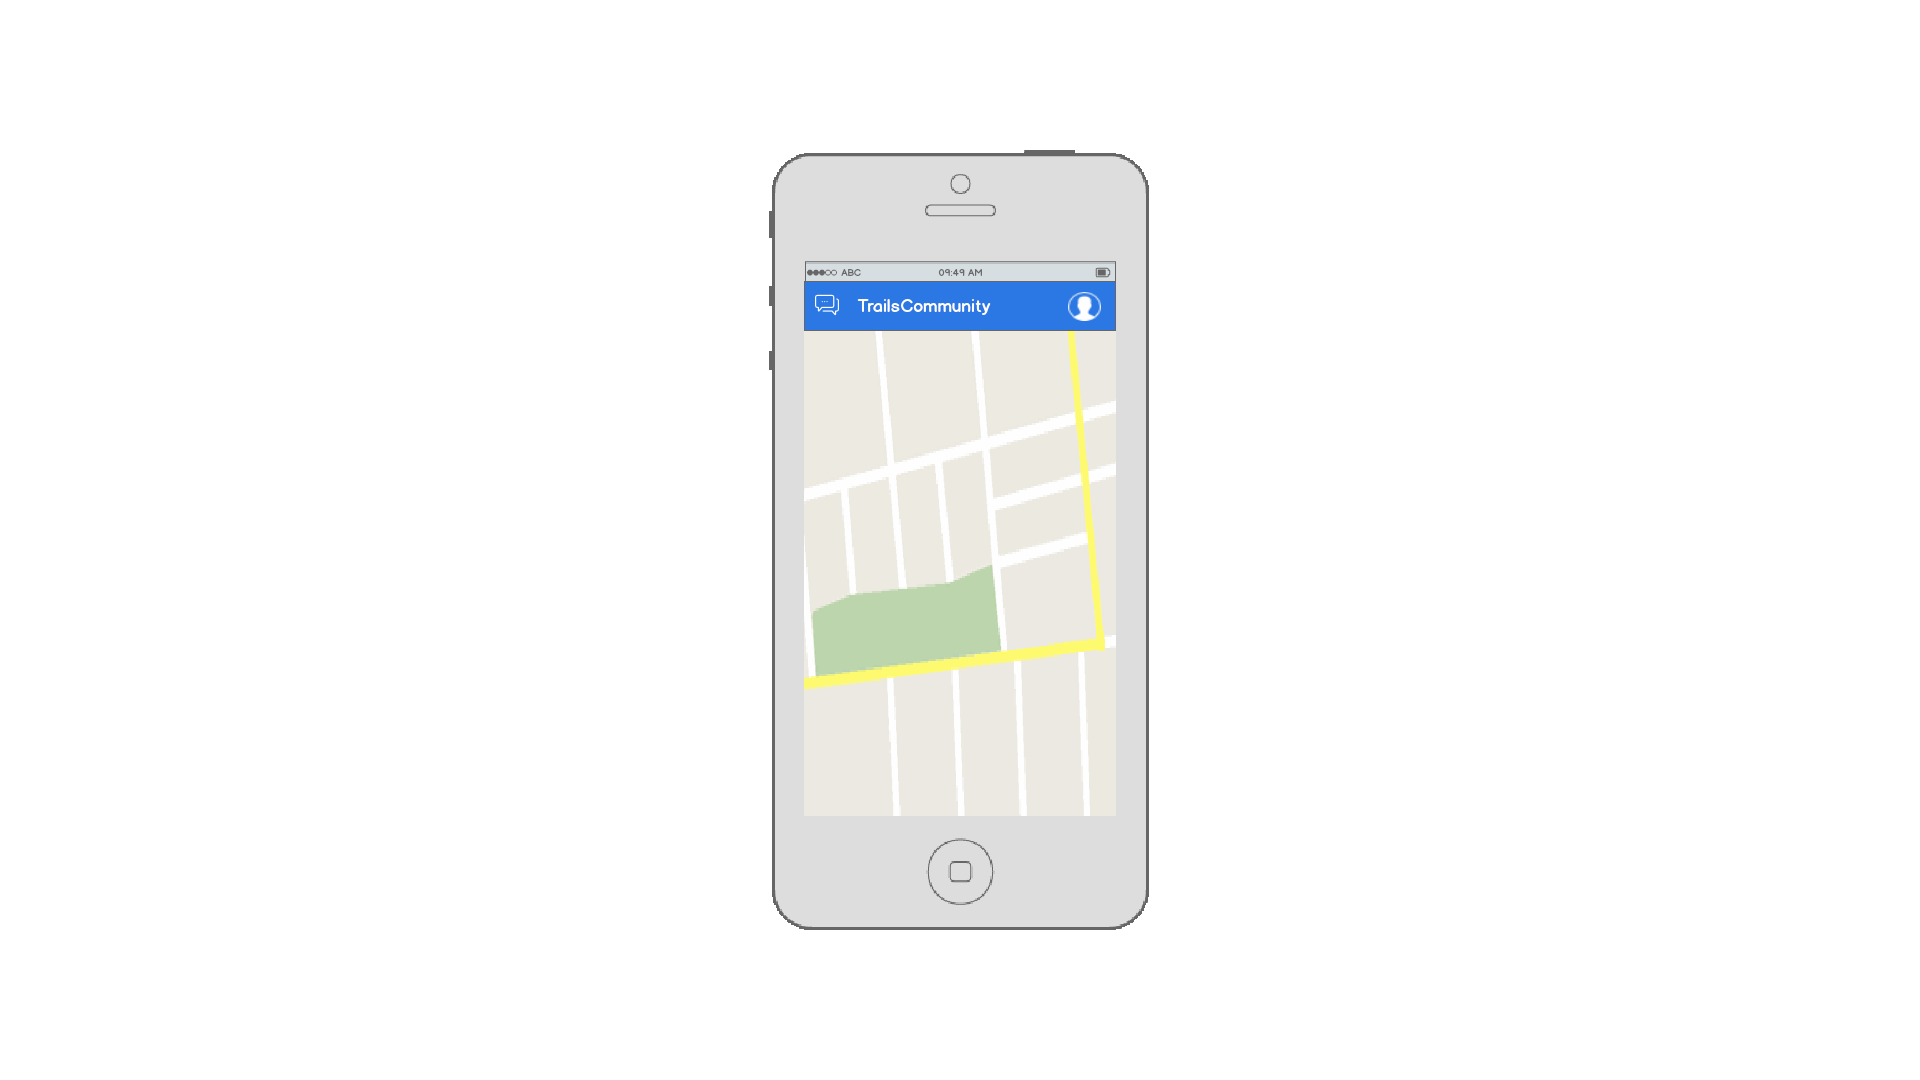
\includegraphics[scale=0.3]{images/mockups/google_map_view.png}
\end{figure}

\clearpage

\paragraph{}La maquette principale est l'affichage des différentes positions des participants de la session courante. Sur cette maquette nous pouvons aussi voir comment l'utilisateur peut accepter ou non un waypoint partagé par un autre participant.

\begin{figure}[!h]
	\caption{Maquette de l'IHM pour l'affichage des différentes positions des participants et de réponse au partage d'un waypoint.}
	\label{session_view}
	\centering
	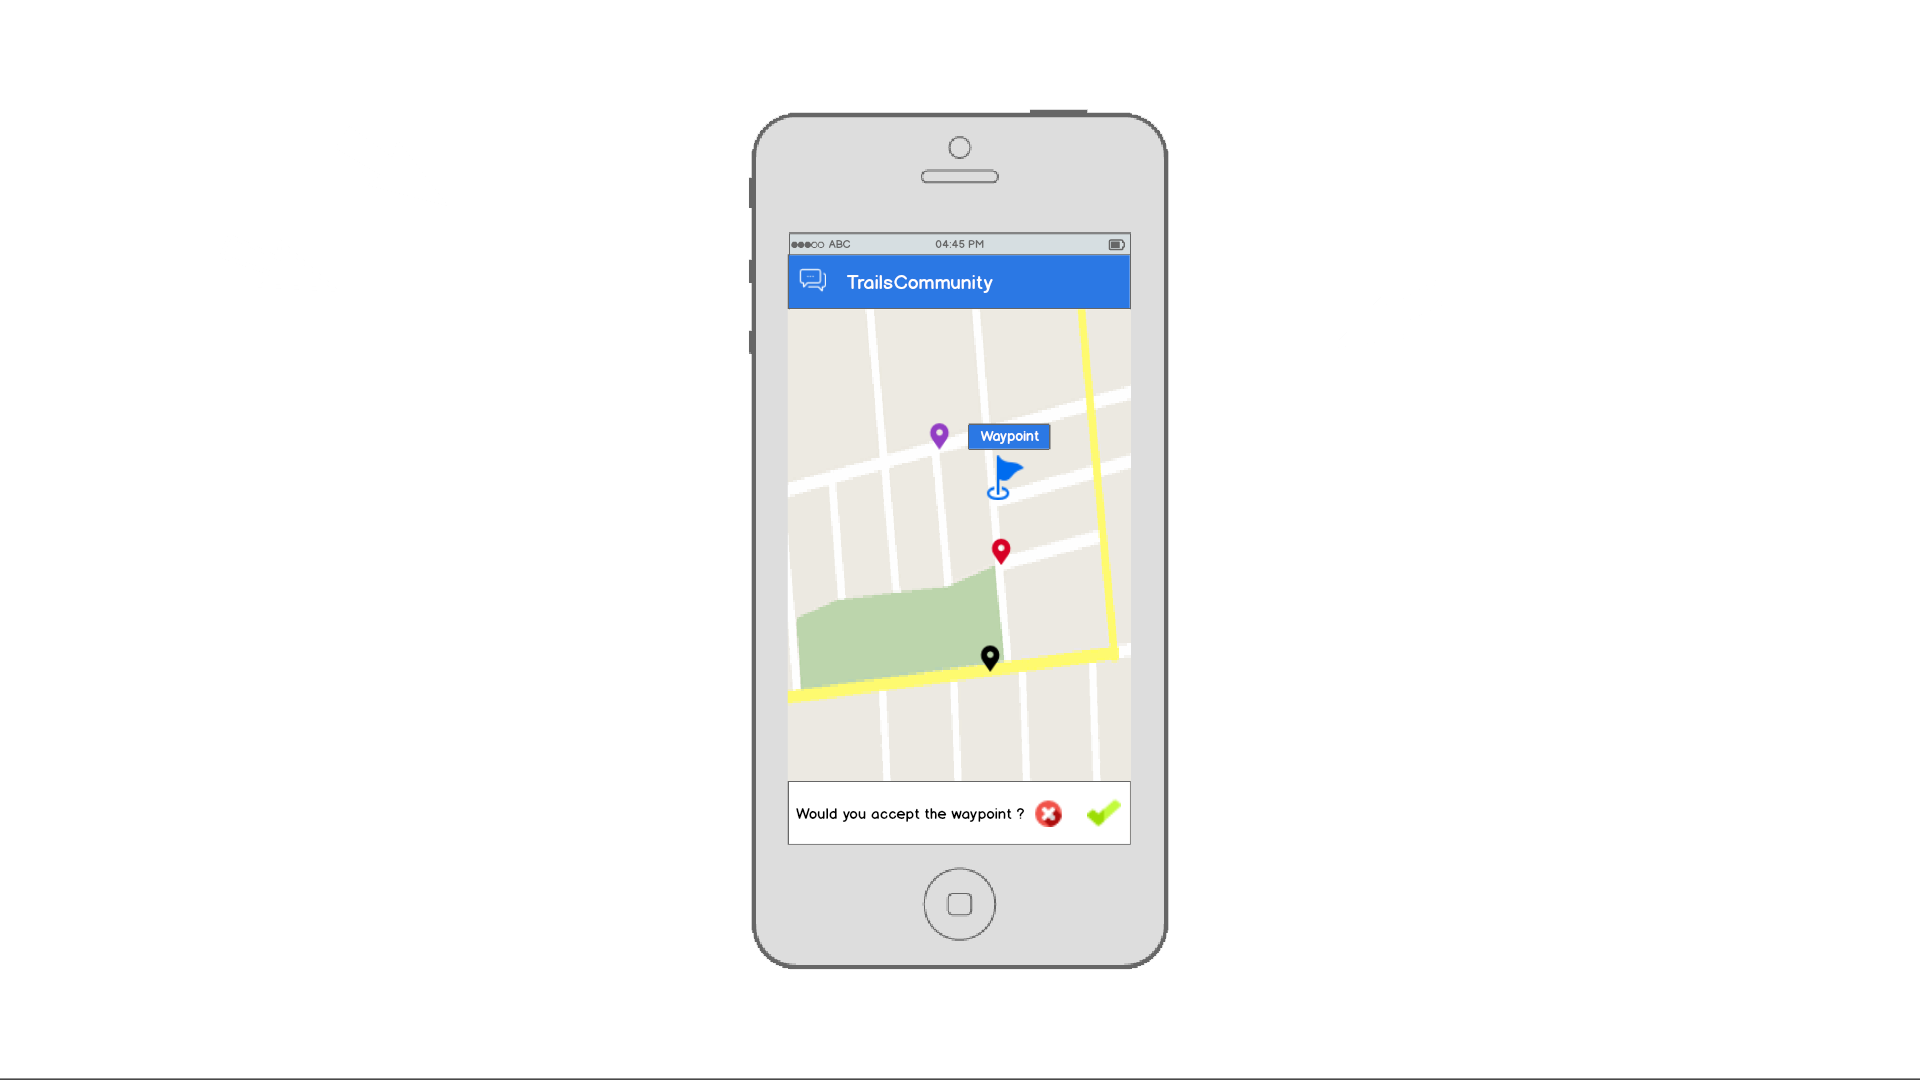
\includegraphics[scale=0.3]{images/mockups/session_marker.png}
\end{figure}

\clearpage

\paragraph{}La maquette suivante présente le chat d'une session courante. La liste des messages ce rafraichi en temps réel.

\begin{figure}[!h]
	\caption{Maquette de l'IHM pour le chat d'une session courante}
	\label{chat_view}
	\centering
	\includegraphics[scale=0.3]{images/mockups/chat.png}
\end{figure}

\clearpage

\paragraph{}Cette maquette montre l'affichage des statistiques de la session courante. Les statistiques apparaissent lors du clique sur le bouton flottant en bas gauche.

\begin{figure}[!h]
	\caption{Maquette de l'IHM pour l'affichage des statistiques d'une session courante}
	\label{statistics_view}
	\centering
	\includegraphics[scale=0.3]{images/mockups/statistics.png}
\end{figure}

\clearpage

\paragraph{}Cette maquette montre l'interface pour que l'organisateur puisse modifier l'ensemble des données de sa session.

\begin{figure}[!h]
	\caption{Maquette de l'IHM pour la modification des données d'une session}
	\label{modify_session}
	\centering
	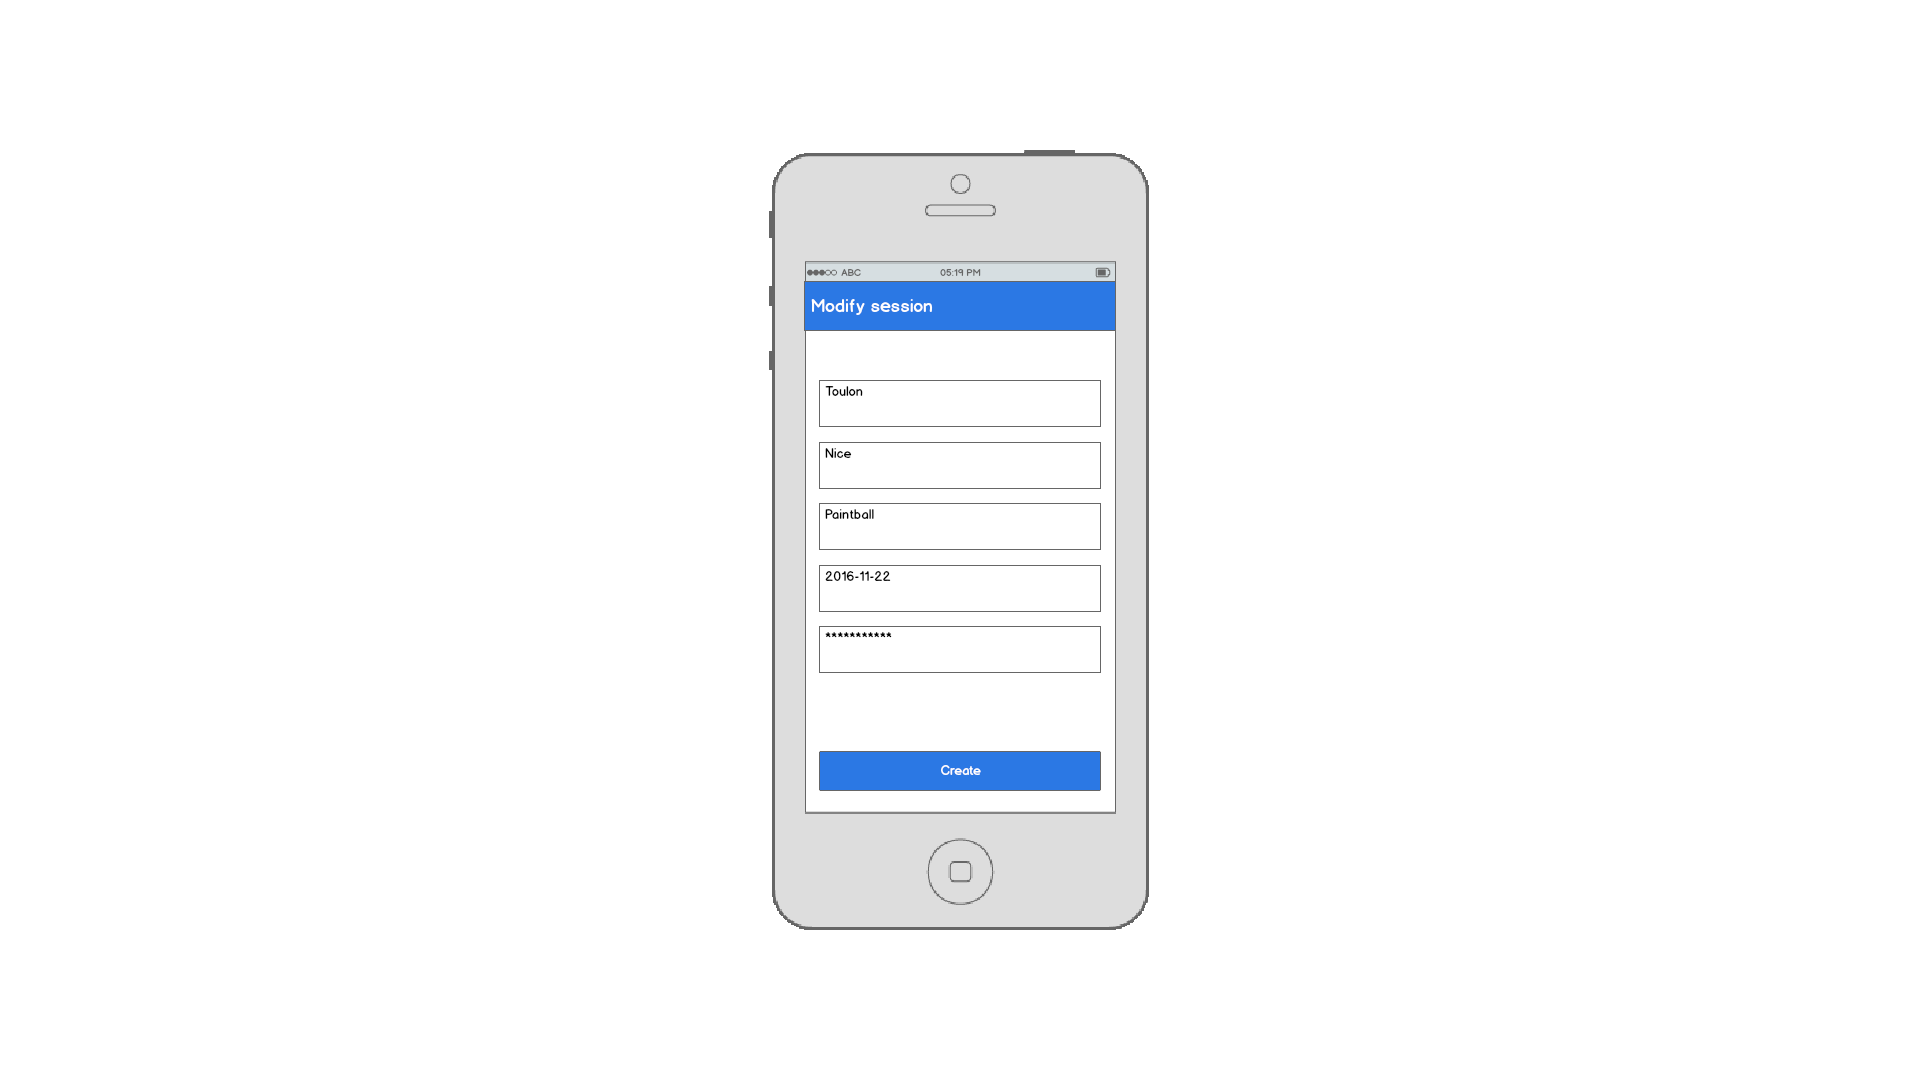
\includegraphics[scale=0.3]{images/mockups/modify_session.png}
\end{figure}

\clearpage

\paragraph{}Cette maquette montre comment un waypoint est diffusé aux autres participants. L'utilisateur a alors le choix d'accepter ou de refuser que le waypoint diffusé apparaisse sur sa Google maps.

\begin{figure}[!h]
	\caption{Maquette de l'IHM pour l'affichage de l'événement d'accepter un nouveau waypoint}
	\label{accept_waypoint}
	\centering
	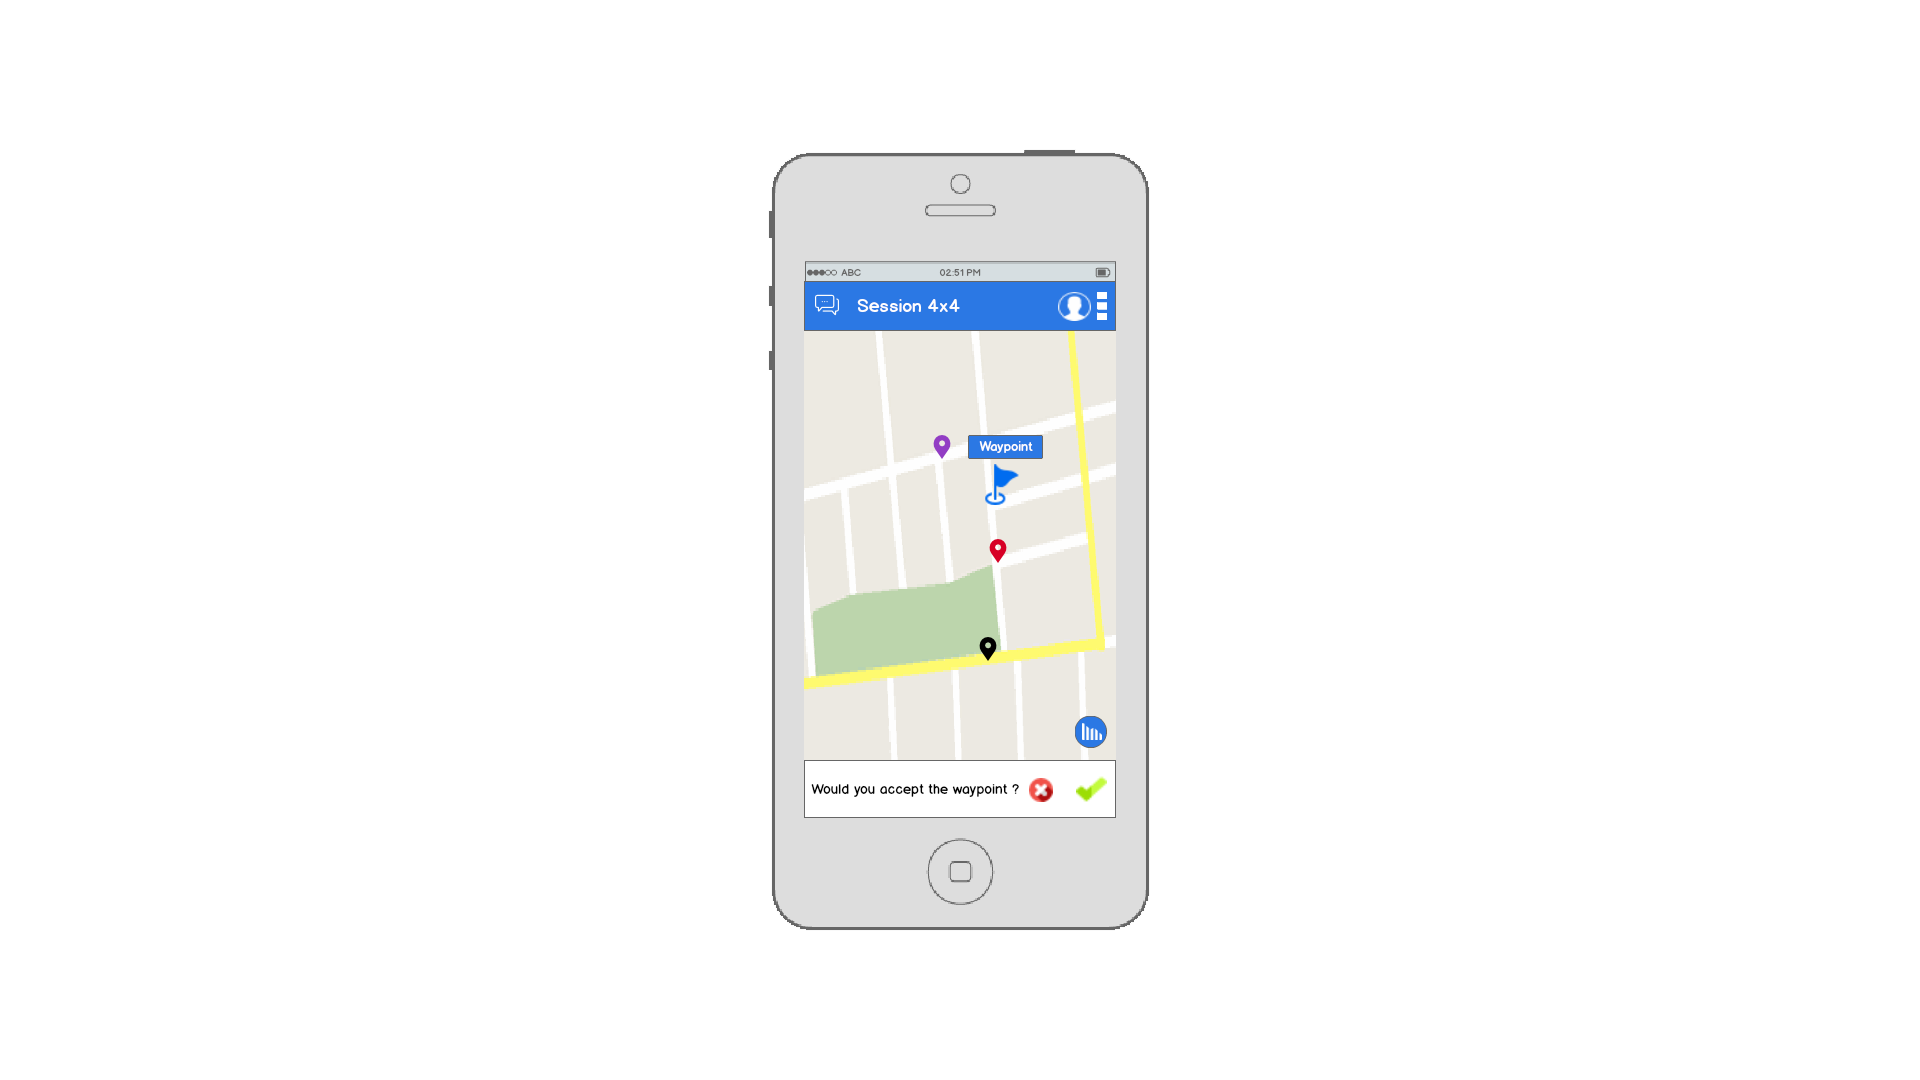
\includegraphics[scale=0.3]{images/mockups/accept_waypoint.png}
\end{figure}

\clearpage

\section{Interfaces matérielles}

\paragraph{}Puisque l'application mobile ne comporte pas de matériel désigné, il n'y a pas d'interfaces matérielles directes. Le GPS physique est géré directement par l'application et la connexion matérielle au serveur est géré par le système d'exploitation sous-jacent sur le téléphone mobile. 

\section{Interfaces logicielles}

\paragraph{}L'application mobile communique avec le GPS pour obtenir les informations géographiques. Pour la localisation de l'utilisateur et la représentation visuelle de celle-ci, l'utilisation du serveur est primordiale afin d'obtenir en temps réel les informations sur les participants.
La communication entre la base de données et l'application se compose des opérations d'écriture et de lecture.

\section{Interfaces de communication}

\paragraph{}La communication entre les différentes parties du système est importante car elles dépendent les unes des autres. Cependant, la manière dont la communication est réalisée n'est pas importante pour le système et est dont traitée par les systèmes d'exploitation pour l'application mobile.

\chapter{Exigences fonctionnelles}

\paragraph{}Cette section comprend les exigences qui spécifient toutes les actions fondamentales du système logiciel.

\section{Visiteur}

\subsection{Exigence fonctionnelle 1.1}

\textbf{ID : FR1}

TITRE : Télécharger l'application mobile.

DESCRIPTION : Un utilisateur doit être en mesure de télécharger l'application mobile via le Google play store. L'application doit être libre de téléchargement.

BUT : Pour qu'un utilisateur puisse télécharger l'application mobile.

DÉPENDANCE : Aucune.

\subsection{Exigence fonctionnelle 1.2}

\textbf{ID : FR2}

TITRE : Télécharger et notifier les utilisateurs des nouvelles versions.

DESCRIPTION : Lorsqu'une nouvelle version/mise à jour est publiée, l'utilisateur doit les vérifier manuellement. Le téléchargement de la nouvelle version devrait se faire via le téléphone mobile de la même manière que le téléchargement de l'application mobile.

BUT : Pour que l'utilisateur puisse télécharger une nouvelle version.

DÉPENDANCE : FR1.

\subsection{Exigence fonctionnelle 1.3}

\textbf{ID : FR3}

TITRE : Enregistrement du visiteur sur l'application mobile.

DESCRIPTION : Étant donné qu'un utilisateur a téléchargé l'application mobile, l'utilisateur devrait pouvoir s'enregistrer via l'application mobile. L'utilisateur doit fournir en premier lieu son surnom puis vient en deuxième, adresse mail ainsi que son mot de passe, le code indicatif téléphonique et pour finir son numéro de téléphone.

BUT : Pour qu'un visiteur puisse s'inscrire sur l'application mobile.

DÉPENDANCE : FR1.

\subsection{Exigence fonctionnelle 1.4}

\textbf{ID : FR4}

TITRE : Connexion du visiteur sur l'application mobile.

DESCRIPTION : Étant donné qu'un visiteur s'est enregistré, il doit pouvoir se connecter à l'application mobile via son adresse mail et son mot de passe. Les informations d'ouverture de session seront stockées dans la base de données. Le mot de passe sera bien sûr crypté côté serveur.

BUT : Pour qu'un visiteur puisse se connecter sur l'application mobile.

DÉPENDANCE : FR1, FR3.

\section{Utilisateur}

\subsection{Exigence fonctionnelle 2.1}

\textbf{ID : FR5}

TITRE : Un utilisateur peut rejoindre une session.

DESCRIPTION : Étant donné qu'un utilisateur s'est connecté, il à le choix entre 3 types de sessions. Le premier type sont les sessions actives, elles sont soit privée ou publique. Si elles sont privées, l'utilisateur doit connaitre le mot de passe pour les rejoindre. Ensuite, le deuxième type est les sessions dont il a déjà participé, cela fonctionne comme un historique. La dernière est les sessions que l'utilisateurs à créées et dont-il est bien sûr l'organisateur.

BUT : Pour qu'un organisateur puisse rejoindre une session sur l'application mobile.

DÉPENDANCE : FR1, FR3, FR4.

\subsection{Exigence fonctionnelle 2.2}

\textbf{ID : FR6}

TITRE : Un utilisateur peut modifier ses données utilisateurs.

DESCRIPTION : Étant donné qu'un utilisateur s'est connecté, il peut modifier ses données utilisateurs. Les champs modifiables sont son pseudonyme, son numéro de téléphone. Les informations des données utilisateur seront stockées dans la base de données.
Dans le cas ou celui-ci les modifient alors qu'il participe à une session. Les autres utilisateurs sont alors notifiés si l'utilisateur modifie son pseudo. La notification apparaitra alors dans le chat.

BUT : Pour qu'un utilisateur puisse modifier ses données utilisateur sur l'application mobile.

DÉPENDANCE : FR1, FR3, FR4.

\subsection{Exigence fonctionnelle 2.3}

\textbf{ID : FR7}

TITRE : Un utilisateur peut se déconnecter de l'application.

DESCRIPTION : Étant donné qu'un utilisateur s'est connecté, il doit avoir le choix, à tout moment de pouvoir se déconnecter de l'application. Il sera alors redirigé vers la page de connexion.

BUT : Pour qu'un organisateur puisse se déconnecter de l'application mobile.

DÉPENDANCE : FR1, FR3.

\section{Participant}

\subsection{Exigence fonctionnelle 3.1}

\textbf{ID : FR8}

TITRE : Un participant peut ajouter un waypoint dans une session active.

DESCRIPTION : Étant donné qu'un participant s'est connecté et à rejoint une session active, il peut ajouter un waypoint. Lorsque l'utilisateur maintient longuement son doigt sur l'écran de son téléphone, un marker est alors ajouté. Le waypoint est alors diffusé à tout les autres participants. Les autres utilisateurs ont alors le choix d'accepter ou de décliner le partage.

BUT : Pour qu'un participant puisse ajouter un waypoint dans une session active.

DÉPENDANCE : FR1, FR3, FR4, FR5.

\subsection{Exigence fonctionnelle 3.2}

\textbf{ID : FR9}

TITRE : Un participant peut communiquer via un système de chat en temps réel à la session courante.

DESCRIPTION : Étant donné qu'un participant s'est connecté et à rejoint une session active, il peut alors communiquer avec l'ensemble des utilisateurs participant à la session. Il lui suffit d'entrer son message et de l'envoyer. Il sera alors diffusé aux autres participants.
De plus, si l'application est hors-ligne. Les messages seront alors envoyé en protocole SMS et stockés dans la base interne pour qu'ils puissent être envoyés au serveur ultérieurement. 

BUT : Pour qu'un participant puisse communiquer via un système de chat en temps réel à la session courante.

DÉPENDANCE : FR1, FR3, FR4, FR5.

\subsection{Exigence fonctionnelle 3.3}

\textbf{ID : FR10}

TITRE : Un participant peut visualiser ses statistiques de la session active.

DESCRIPTION : Étant donné qu'un participant s'est connecté et à rejoint une session active, il peut alors visualiser l'ensemble de ses statistiques. Celle-ci décrivent différentes données comme la distance total parcouru, la vitesse moyenne du participant ou alors le nombre de waypoint ajoutés. 

BUT : Pour qu'un participant puisse visualiser ses statistiques de la session active

DÉPENDANCE : FR1, FR3, FR4, FR5.


\section{Organisateur}

\subsection{Exigence fonctionnelle 4.1}

\textbf{ID : FR11}

TITRE : Un organisateur peut créer une session.

DESCRIPTION : Étant donné qu'un organisateur s'est connecté, il doit pouvoir créer une nouvelle session dans l'application. Les informations de la nouvelle session créée seront stockées dans la base de données du serveur distant. L'organisateur doit fournir le lieu de départ ainsi que le lieu d'arrivé. Le format d'une adresse lui sera demandé. L'application convertira cette adresse en coordonnées GPS. De plus, il devra indiquer le type d'activité ainsi que la date de départ. Pour finir,  l'organisateur aura la possibilité de verrouiller la session par un mot de passe qu'il divulguera à l'ensemble des participants.

BUT : Pour qu'un organisateur puisse créer une session sur l'application mobile.

DÉPENDANCE : FR1, FR3, FR4.

\subsection{Exigence fonctionnelle 4.2}

\textbf{ID : FR12}

TITRE : Un organisateur peut gérer ses sessions.

DESCRIPTION : Étant donné qu'un organisateur s'est connecté, il doit pouvoir gérer ses sessions. Touts les champs remplis précédemment lors de la création de la session sont modifiables. Les informations de la session seront stockées dans la base de données.

BUT : Pour qu'un organisateur puisse gérer une session sur l'application mobile.

DÉPENDANCE : FR1, FR3, FR4, FR5.

\subsection{Exigence fonctionnelle 4.3}

\textbf{ID : FR13}

TITRE : Un organisateur peut clôturer ses sessions.

DESCRIPTION : Étant donné qu'un organisateur s'est connecté et à sélectionné une de ses sessions créées précédemment. Il doit pouvoir clôturer la session sélectionné. Celle-ci n'est alors plus présente dans les sessions actives de l'application sauf pour les participants où la session est alors disponible dans leurs historiques. Cette action est disponible dans le menu déroulant des trois petits points (voir maquette 3.7). Une boîte de dialogue de confirmation va alors apparaitre pour qu'il puisse confirmer ou annuler son action.

BUT : Pour qu'un organisateur puisse clôturer une session sur l'application mobile.

DÉPENDANCE : FR1, FR3, FR4, FR5.

\section{Application}

\subsection{Exigence fonctionnelle 5.1}

\textbf{ID : FR14}

TITRE : L'application doit pouvoir enregistrer un parcours effectué sans connexion internet.

DESCRIPTION : Étant donné qu'un utilisateur s'est connecté, a rejoint une session active et qu'il est déconnecté du réseau internet, l'application doit pouvoir gérer le mode hors ligne. Une base de données interne a l'application va alors stockée l'ensemble des données. Lorsque l'utilisateur sera de nouveau connecté, les informations seront alors synchronisé avec le serveur.

BUT : Pour que l'application puisse pouvoir enregistrer un parcours effectué sans connexion internet. 

DÉPENDANCE : FR1, FR3, FR4, FR5.

\subsection{Exigence fonctionnelle 5.2}

\textbf{ID : FR15}

TITRE : Le chat de l'application doit pouvoir fonctionné en mode hors ligne.

DESCRIPTION : Étant donné qu'un utilisateur s'est connecté, à rejoint une session active et qu'il est déconnecté du réseau internet, l'application doit pouvoir gérer le mode hors ligne du chat. L'application va alors basculée sur le protocole SMS pour que les participants puissent continués de communiquer ensemble. De plus, l'ensemble des messages seront stocké en internet et synchronisé avec le serveur lorsque l'utilisateur sera de nouveau en ligne.

BUT : Pour que le chat de l'application puisse fonctionner en mode hors ligne.

DÉPENDANCE : FR1, FR3, FR4, FR5.

\section{IHM}

\subsection{Exigence fonctionnelle 6.1}

\textbf{ID : FR16}

TITRE : Le système doit pouvoir afficher une carte Google maps interactive.

DESCRIPTION : Le système doit être capable d'afficher une carte Google maps interactive. En effet, cette carte doit pouvoir posséder les fonctionnalités de zoom ainsi qu'une navigation tactile et ergonomique.

BUT : Pour que le système puisse afficher une carte Google maps interactive.

DÉPENDANCE : Aucune.

\subsection{Exigence fonctionnelle 6.2}

\textbf{ID : FR17}

TITRE : Le système doit pouvoir ajouter un ou plusieurs markers sur une carte Google maps.

DESCRIPTION : Étant donné que le système a affiché une carte Google maps interactive, il doit permettre de pouvoir ajouter un ou plusieurs markers sur celle-ci. En effet ces markers peuvent posséder un titre interactif qui, lors d'une appuie, peuvent afficher une multitude d'informations supplémentaires sur le marker associé.

BUT : Pour que le système puisse ajouter un ou plusieurs markers sur une carte Google maps.

DÉPENDANCE : F16.

\subsection{Exigence fonctionnelle 6.3}

\textbf{ID : FR18}

TITRE : Le système doit pouvoir afficher un ou plusieurs parcours sur une carte Google maps.

DESCRIPTION : Étant donné que le système a affiché une carte Google maps interactive, il doit permettre de pouvoir afficher un ou plusieurs parcours sur celle-ci. En effet ces chemins possède un marker de début et un marker de fin pour signaler aux autres participants où ce situe l'utilisateur. Ce parcours possèdera une couleur unique dans la session active.

BUT : Pour que le système puisse afficher un ou plusieurs parcours sur une carte Google map.

DÉPENDANCE : F16, F17.

\subsection{Exigence fonctionnelle 6.4}

\textbf{ID : FR19}

TITRE : Le système doit pouvoir afficher la géo-localisation des participants d'une session active sur une carte Google maps.

DESCRIPTION : Étant donné que le système a affiché une carte Google maps interactive, il doit permettre de pouvoir afficher la géo-localisation des participants d'une session active sur celle-ci. En effet cette géo-localisation est signalé par un marker au bout du chemin associé aux participants. Cette géo-localisation est réalisé par le GPS interne du téléphone portable. De plus, la précision de la celle-ci dépendra totalement du système d'exploitation et du matériel du téléphone portable de l'utilisateur. 

BUT : Pour que le système puisse afficher la géo-localisation des participants d'une session active sur une carte Google maps.

DÉPENDANCE : F16.

\subsection{Exigence fonctionnelle 6.5}

\textbf{ID : FR20}

TITRE : Le système doit pouvoir afficher différentes unités de mesures des statistiques en fonction des activités.

DESCRIPTION : Le système doit pouvoir afficher différentes unités de mesures en fonction du type d'activité. En effet, les mesures sont différentes pour une activité ce réalisant avec une voiture et une activité ce réalisant en bateau ou à pied. Le système va alors déterminer en fonction du type d'activité choisit l'unité de mesure le plus adéquate.

BUT : Pour que le système puisse afficher différentes unités de mesures des statistiques en fonction des activités.

DÉPENDANCE : Aucune.

\subsection{Exigence fonctionnelle 6.6}

\textbf{ID : FR21}

TITRE : Le système doit pouvoir gérer la gestion un mode multi-session.

DESCRIPTION : Le système doit permettre un système de multi-session. Il permettra a l'utilisateur de pouvoir utiliser son compte sur différent mobile.

BUT : Pour que le système puisse gérer un mode multi-session.

DÉPENDANCE : Aucune.

\section{Performances}

\subsection{Exigence fonctionnelle 7.1}

\textbf{ID : FR22}

TITRE : Le système doit afficher rapidement l'ensemble des sessions dans les listes déroulantes.

DESCRIPTION : Le système doit posséder un niveau de performance élevé pour l'affichage des différentes sessions envoyé par le serveur. En effet, la rapidité d'affichage doit être rapide et aucune latence ne doit être observé par l'utilisateur. De plus, un maximum de 50 sessions actives sera affichées. 

BUT : Pour que le système puisse afficher rapidement l'ensemble des sessions dans les listes déroulantes.

DÉPENDANCE : Aucune.

\subsection{Exigence fonctionnelle 7.2}

\textbf{ID : FR23}

TITRE : Le système doit afficher rapidement l'ensemble des différents éléments affichés sur la carte Google maps interactive.

DESCRIPTION : Le système doit posséder un niveau de performance élevé pour l'affichage des différents éléments affichés sur la carte Google maps. En effet, aucune latence ne doit être observé par l'utilisateur lors de la réception de coordonnées GPS ou l'affichage d'un nouveau waypoint. De plus, l'affichage des parcours de l'ensemble des participants d'une session active ne doit pas entrainer une surcharge du serveur. 

BUT : Pour que le système puisse afficher rapidement l'ensemble des différents éléments affichés sur la carte Google maps interactive.

DÉPENDANCE : Aucune.

\subsection{Exigence fonctionnelle 7.3}

\textbf{ID : FR24}

TITRE : Le serveur doit posséder un temps de réponse inférieur à une seconde.

DESCRIPTION : Le serveur doit posséder un temps de réponse inférieur à une seconde. Ce temps est un temps de performance idéal cependant, le temps de réponse doit être au minimum inférieur à deux secondes.  

BUT : Pour que le serveur doit posséder un temps de réponse inférieur à une seconde.

DÉPENDANCE : Aucune.

\section{Sécurité}

\subsection{Exigence fonctionnelle 7.1}

\textbf{ID : FR25}

ESSENTIEL : La sécurité de création de compte pour les utilisateurs du système.

DESCRIPTION : Si un utilisateur veut créer un compte et que le nom de l'utilisateur souhaité est déjà utilisé, l'utilisateur va être invité à choisir un nom d'utilisateur différent.

NIVEAU : Haute.

\subsection{Exigence fonctionnelle 7.2}

\textbf{ID : FR26}

ESSENTIEL : La sécurité de la communication entre le système et le serveur.

DESCRIPTION : Les messages doivent être chiffrés pour les communications de connexion, de sorte que d'autres utilisateurs ne peuvent pas obtenir le nom d'utilisateur et le mot de passe à partir de ces messages.

NIVEAU : Haute.

\subsection{Exigence fonctionnelle 7.3}

\textbf{ID : FR27}

ESSENTIEL : Le nombre de requête par seconde côté serveur.

DESCRIPTION : Le serveur peut ajouter une limitation de requête par seconde pour un utilisateur. Cela permet d'évité les attaques de brute forces et autre attaques d'injection de code.

NIVEAU : Haute.

\subsection{Exigence fonctionnelle 7.4}

\textbf{ID : FR28}

ESSENTIEL : Utilisation d’un token pour la communication client-serveur.

DESCRIPTION : Les échanges entre client-serveur se fait grâce à un token généré par le serveur. Ce token est unique et propre à chaque utilisateur. L'utilisation de ce token permet de sécuriser les ressources du serveur. A chaque requête, le token doit être présent dans l'en-tête. S'il n'y a pas de token, le serveur renvoie une réponse comme quoi l'utilisateur n'est pas autorisé à accéder à cette ressource.

NIVEAU : Haute.


\chapter{Conception UML}

\section{Modélisation de l'axe statique}

\subsection{Diagramme de contexte statique}

\paragraph{}Nous distinguons quatre types d'acteurs : un visiteur, un utilisateur, un participant et un organisateur. Chaque acteurs auront des utilisations de l'application mobile complètement distincts. 

\begin{figure}
	\caption{Diagramme de contexte statique}
	\label{statique_diagram}
	\centering
	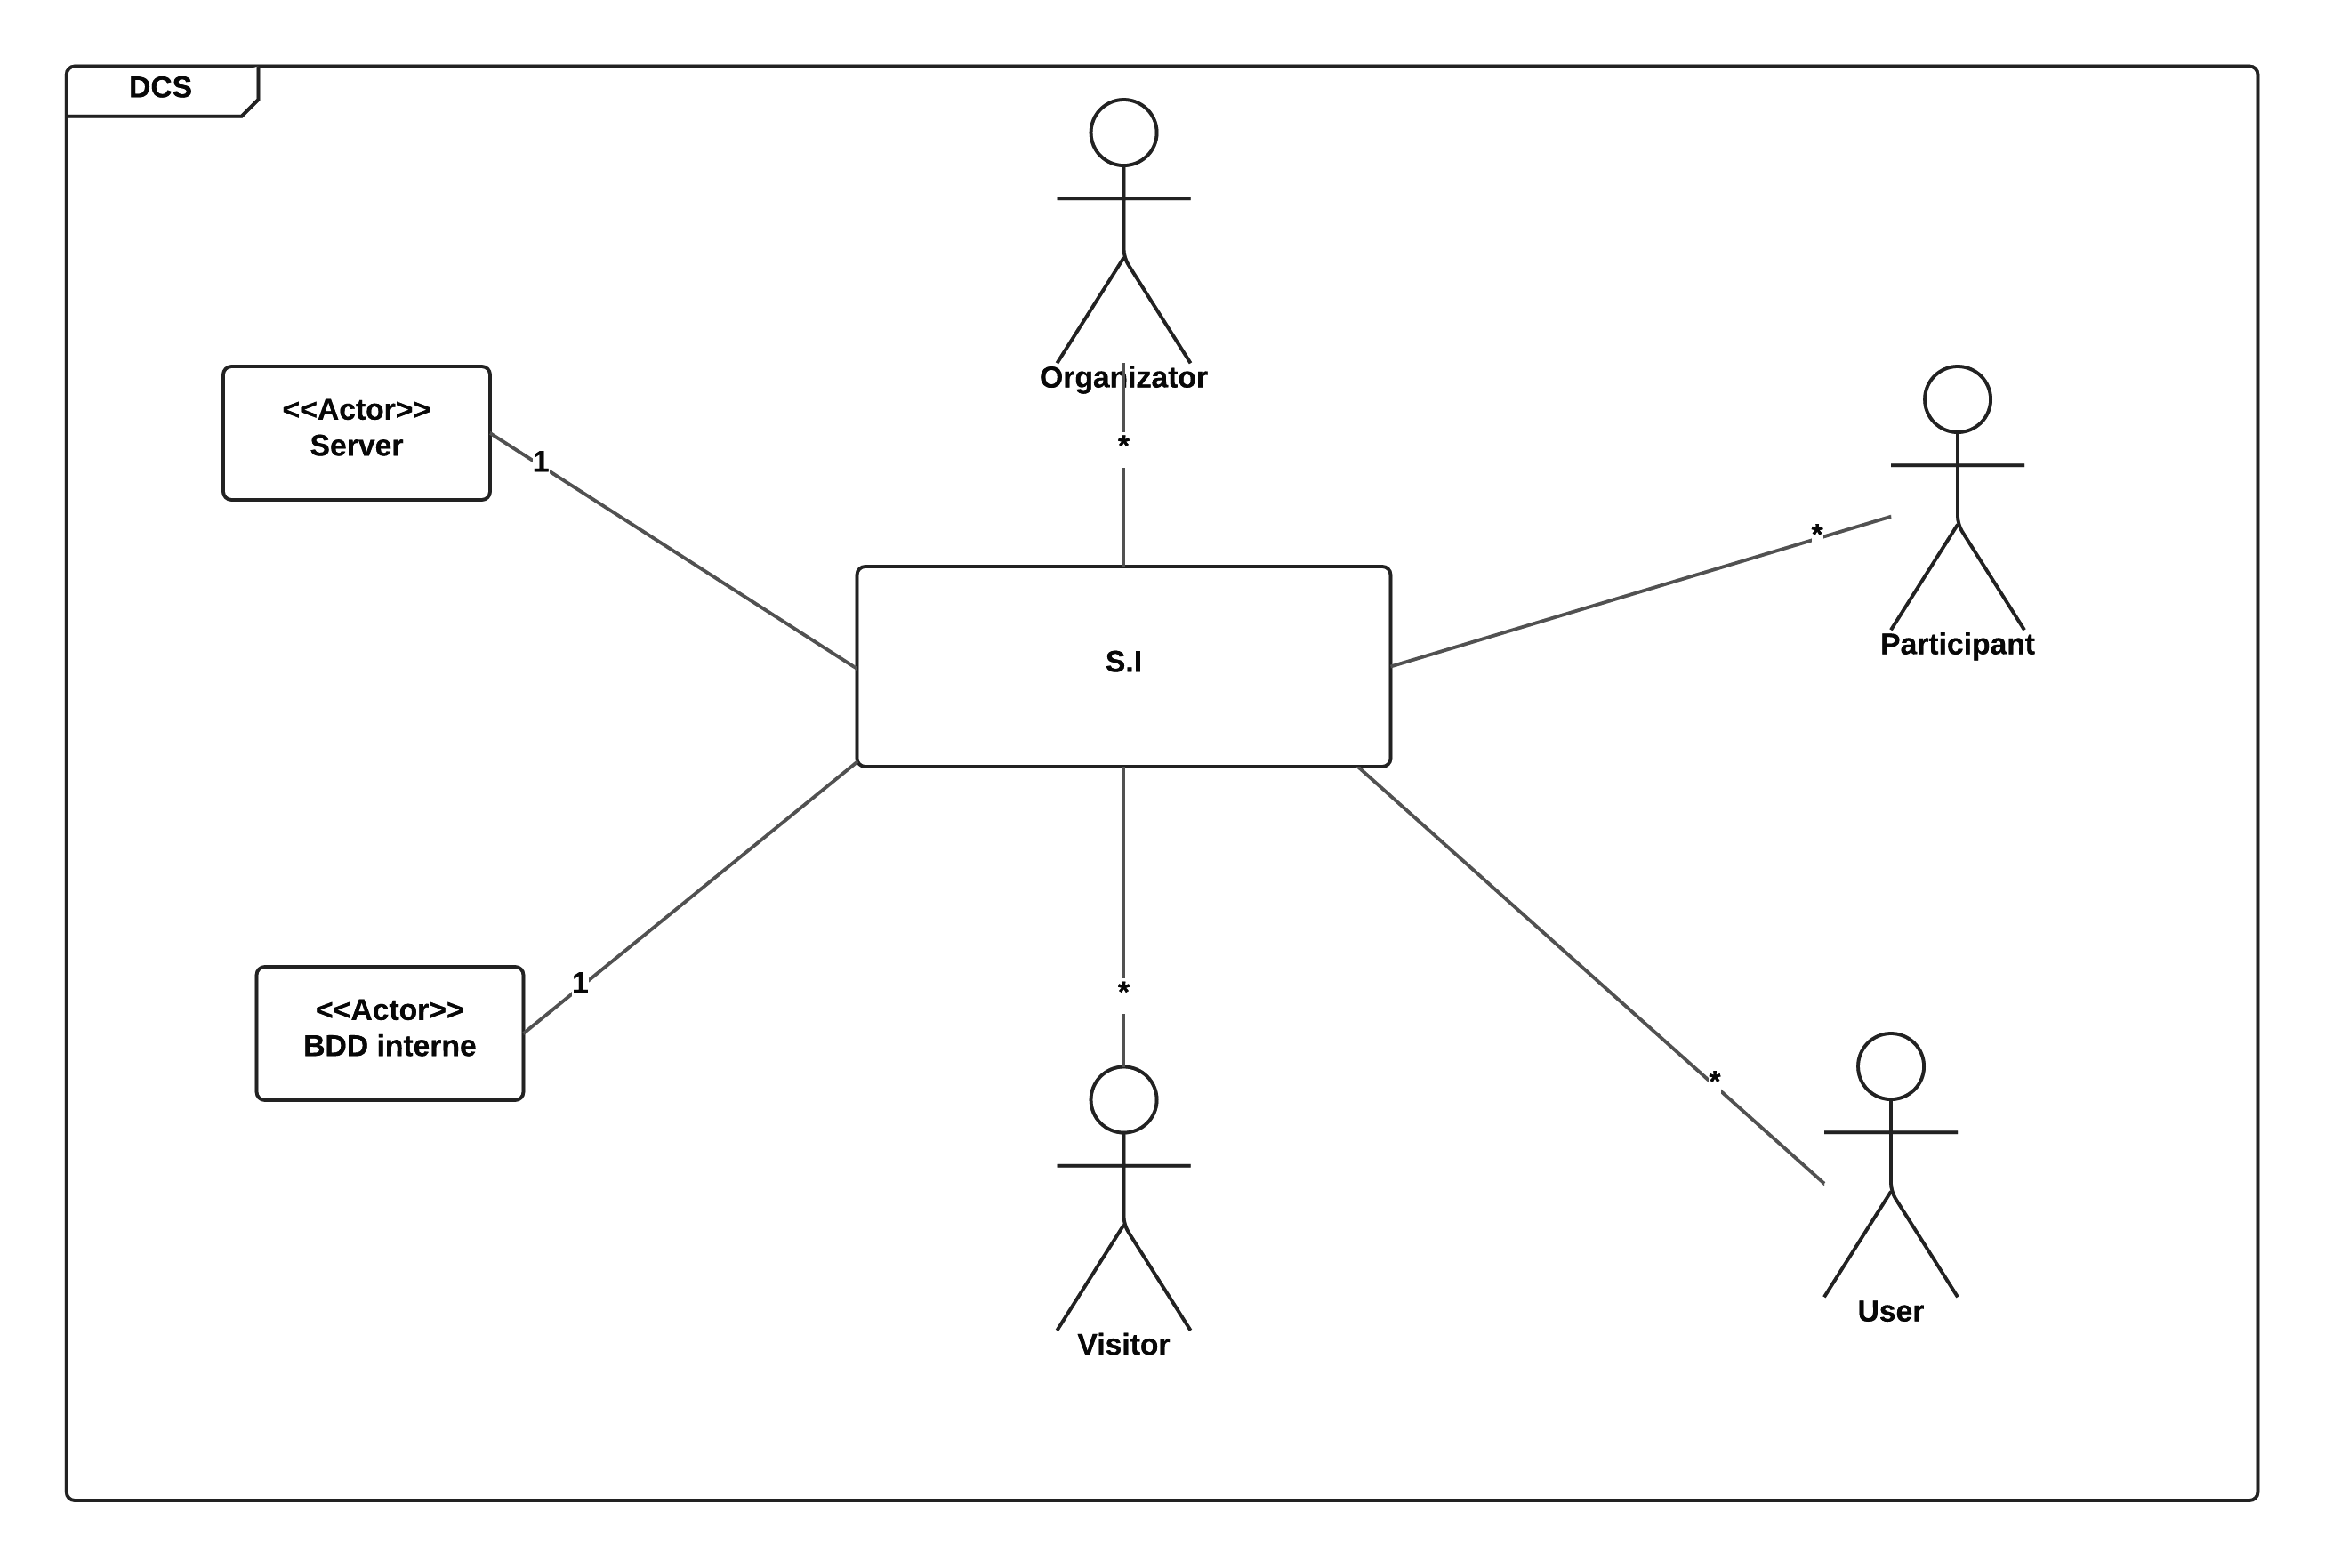
\includegraphics[scale=0.2]{Images/diagram/static_diagram.png}
\end{figure}

\clearpage

\paragraph{}L'accès aux données nécessaires au fonctionnement de l'application se fera par le biais d'un serveur codé en Ruby dont le fonctionnement est détaillé en annexe. C'est ce serveur qui communiquera avec la base de données qui stocke l'ensemble des informations des sessions.

\subsection{Diagramme des cas d'utilisation}

\paragraph{}L'ensemble des cas d'usages excepté la création d'un compte utilisateur requière une authentification. Le statut de l'acteur diffère en fonction des actions qu'il réalise sur l'application. 

\begin{figure}[!h]
	\caption{Diagramme des cas d'utilisation}
	\label{use_case_diagram}
	\centering
	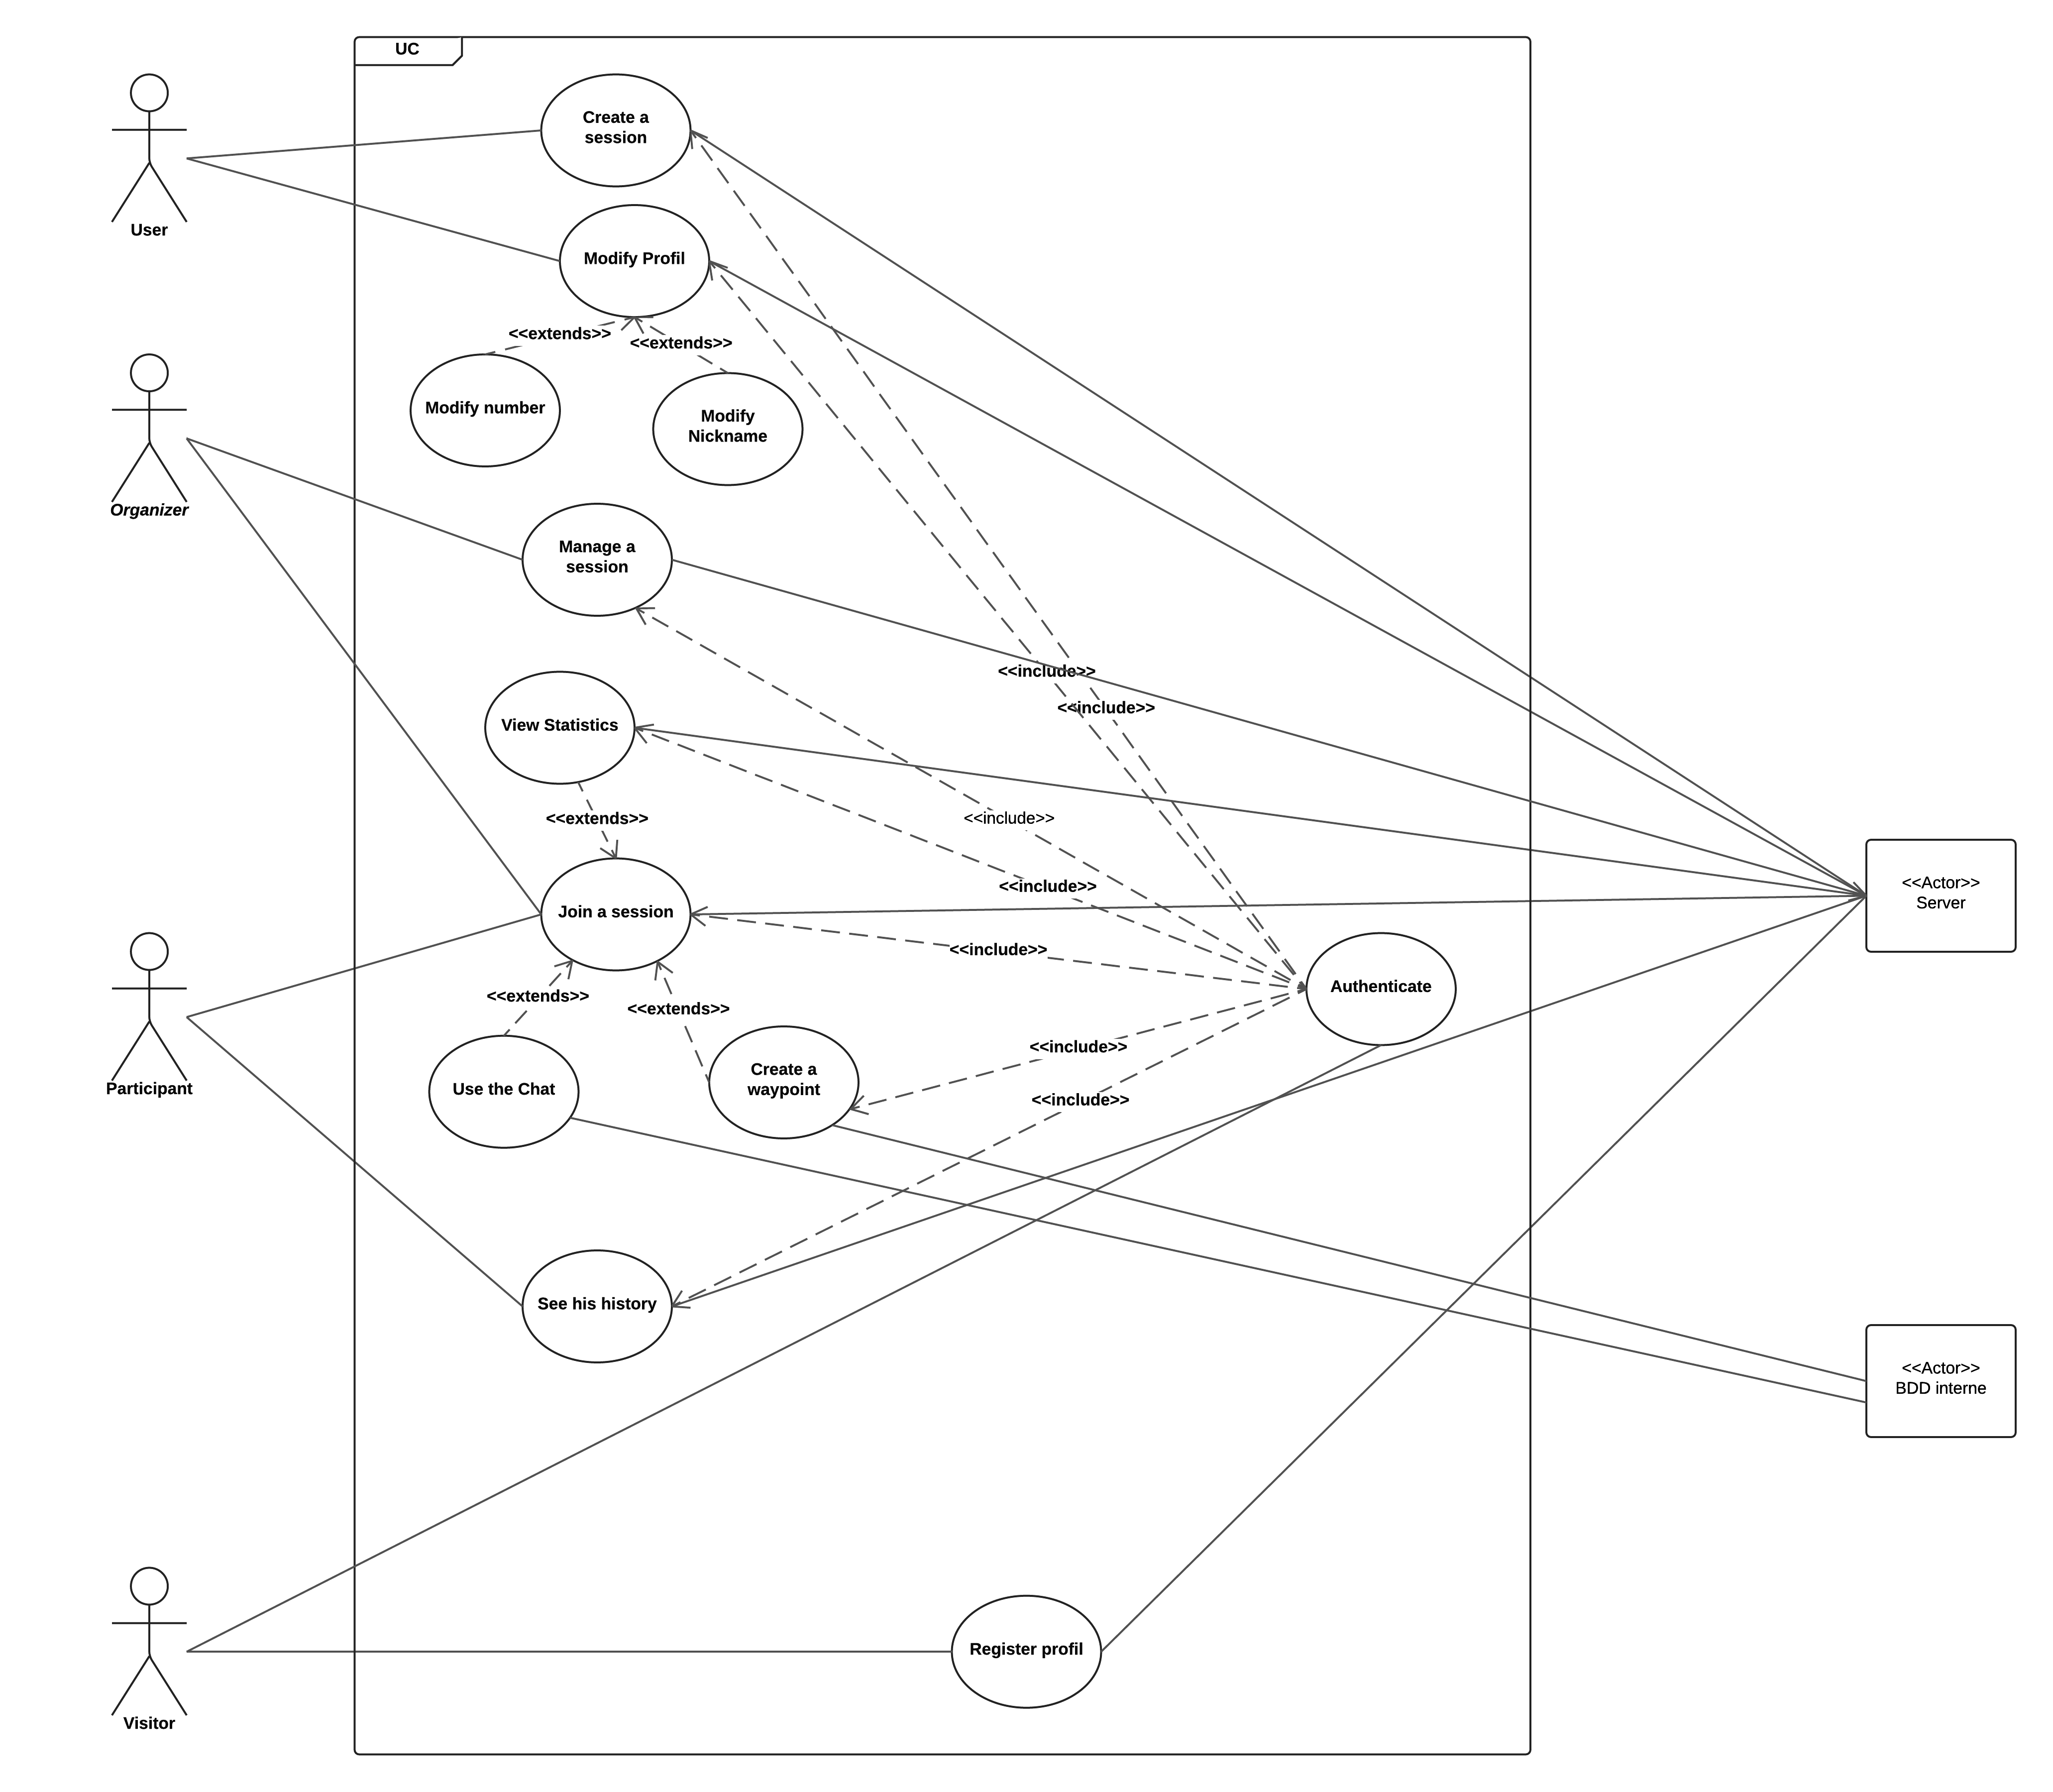
\includegraphics[scale=0.5]{Images/diagram/use_case_diagram.png}
\end{figure}

\clearpage

\paragraph{}La priorité des cas d'utilisation est détaillée dans un tableau des priorités plus bas bans le rapport. La principal fonctionnalité de l'application est d'assurer la possibilité de créer une session d'une activité quelconque et d'y participer.

\begin{center}
	\begin{tabular}{|c|c|c|}
		\hline
		Use case & Priority & Risk \\ \hline
		Create a session & High & High \\ \hline
		Manage a session & High & High \\ \hline
		Join a session & High & Mean \\ \hline
		Create a waypoint & Mean & Mean \\ \hline
		Authentification & Mean & Mean \\ \hline
		Use the chat & Low & Low \\ \hline
		See statistics & Low & Low \\ \hline
		See his history & Low & Low \\ \hline
		Modify profil & Low & Low \\
		\hline \hline
	\end{tabular}
\end{center}

\subsection{Diagramme de classe}

%Diagramme de classe%

\subsection{Diagramme entité association}

\begin{figure}[!h]
	\caption{Diagramme entité association}
	\label{database_ERD}
	\centering
	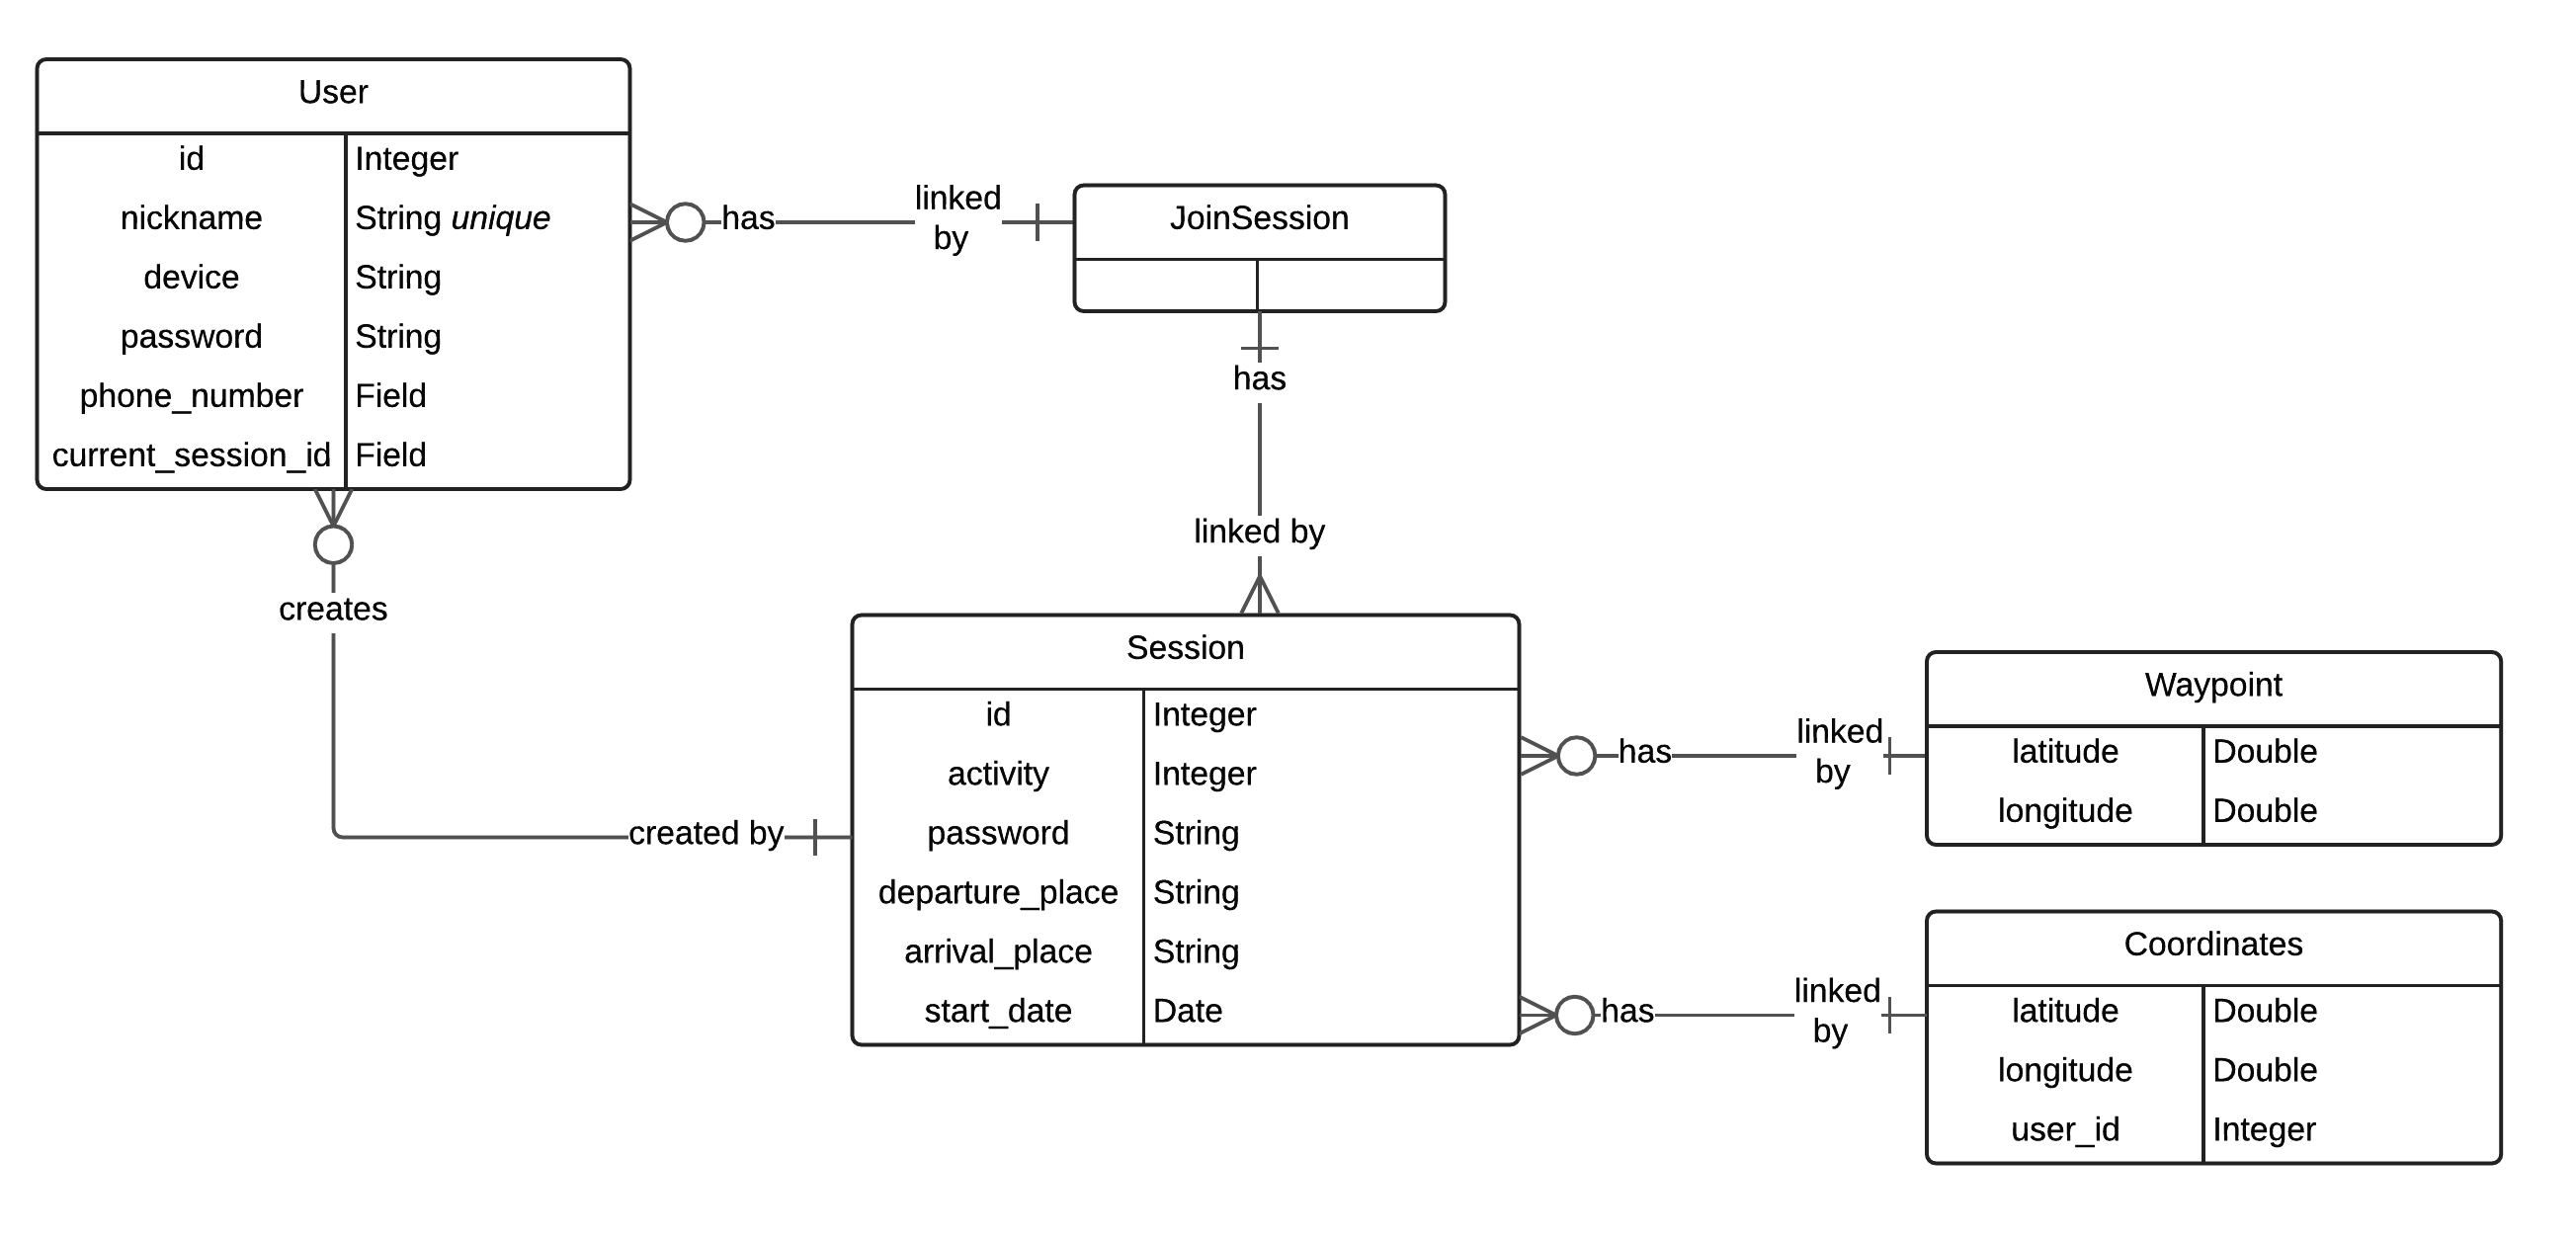
\includegraphics[scale=0.7]{Images/diagram/database_ERD.png}
\end{figure}

\section{Modélisation des axes fonctionnel et dynamique}

\subsection{Généralités}

\paragraph{}Tous les diagrammes de séquences et d'activités présentés ci-dessous seront depuis le point de vue du client.
\paragraph{}Une rapide modélisation du serveur sera présente dans la partie "Modélisation du serveur".
\paragraph{}Tous les cas d'utilisation débutent nécessairement par une connexion de l'utilisateur.
\paragraph{}De plus l'ensemble des données sont testées sur le client mais aussi sur le serveur qui contient la base de données.

%Diagramme de séquence authentification%

\begin{figure}[!h]
	\caption{Diagramme de séquence authentification}
	\label{authentification_sequence_diagram}
	\centering
	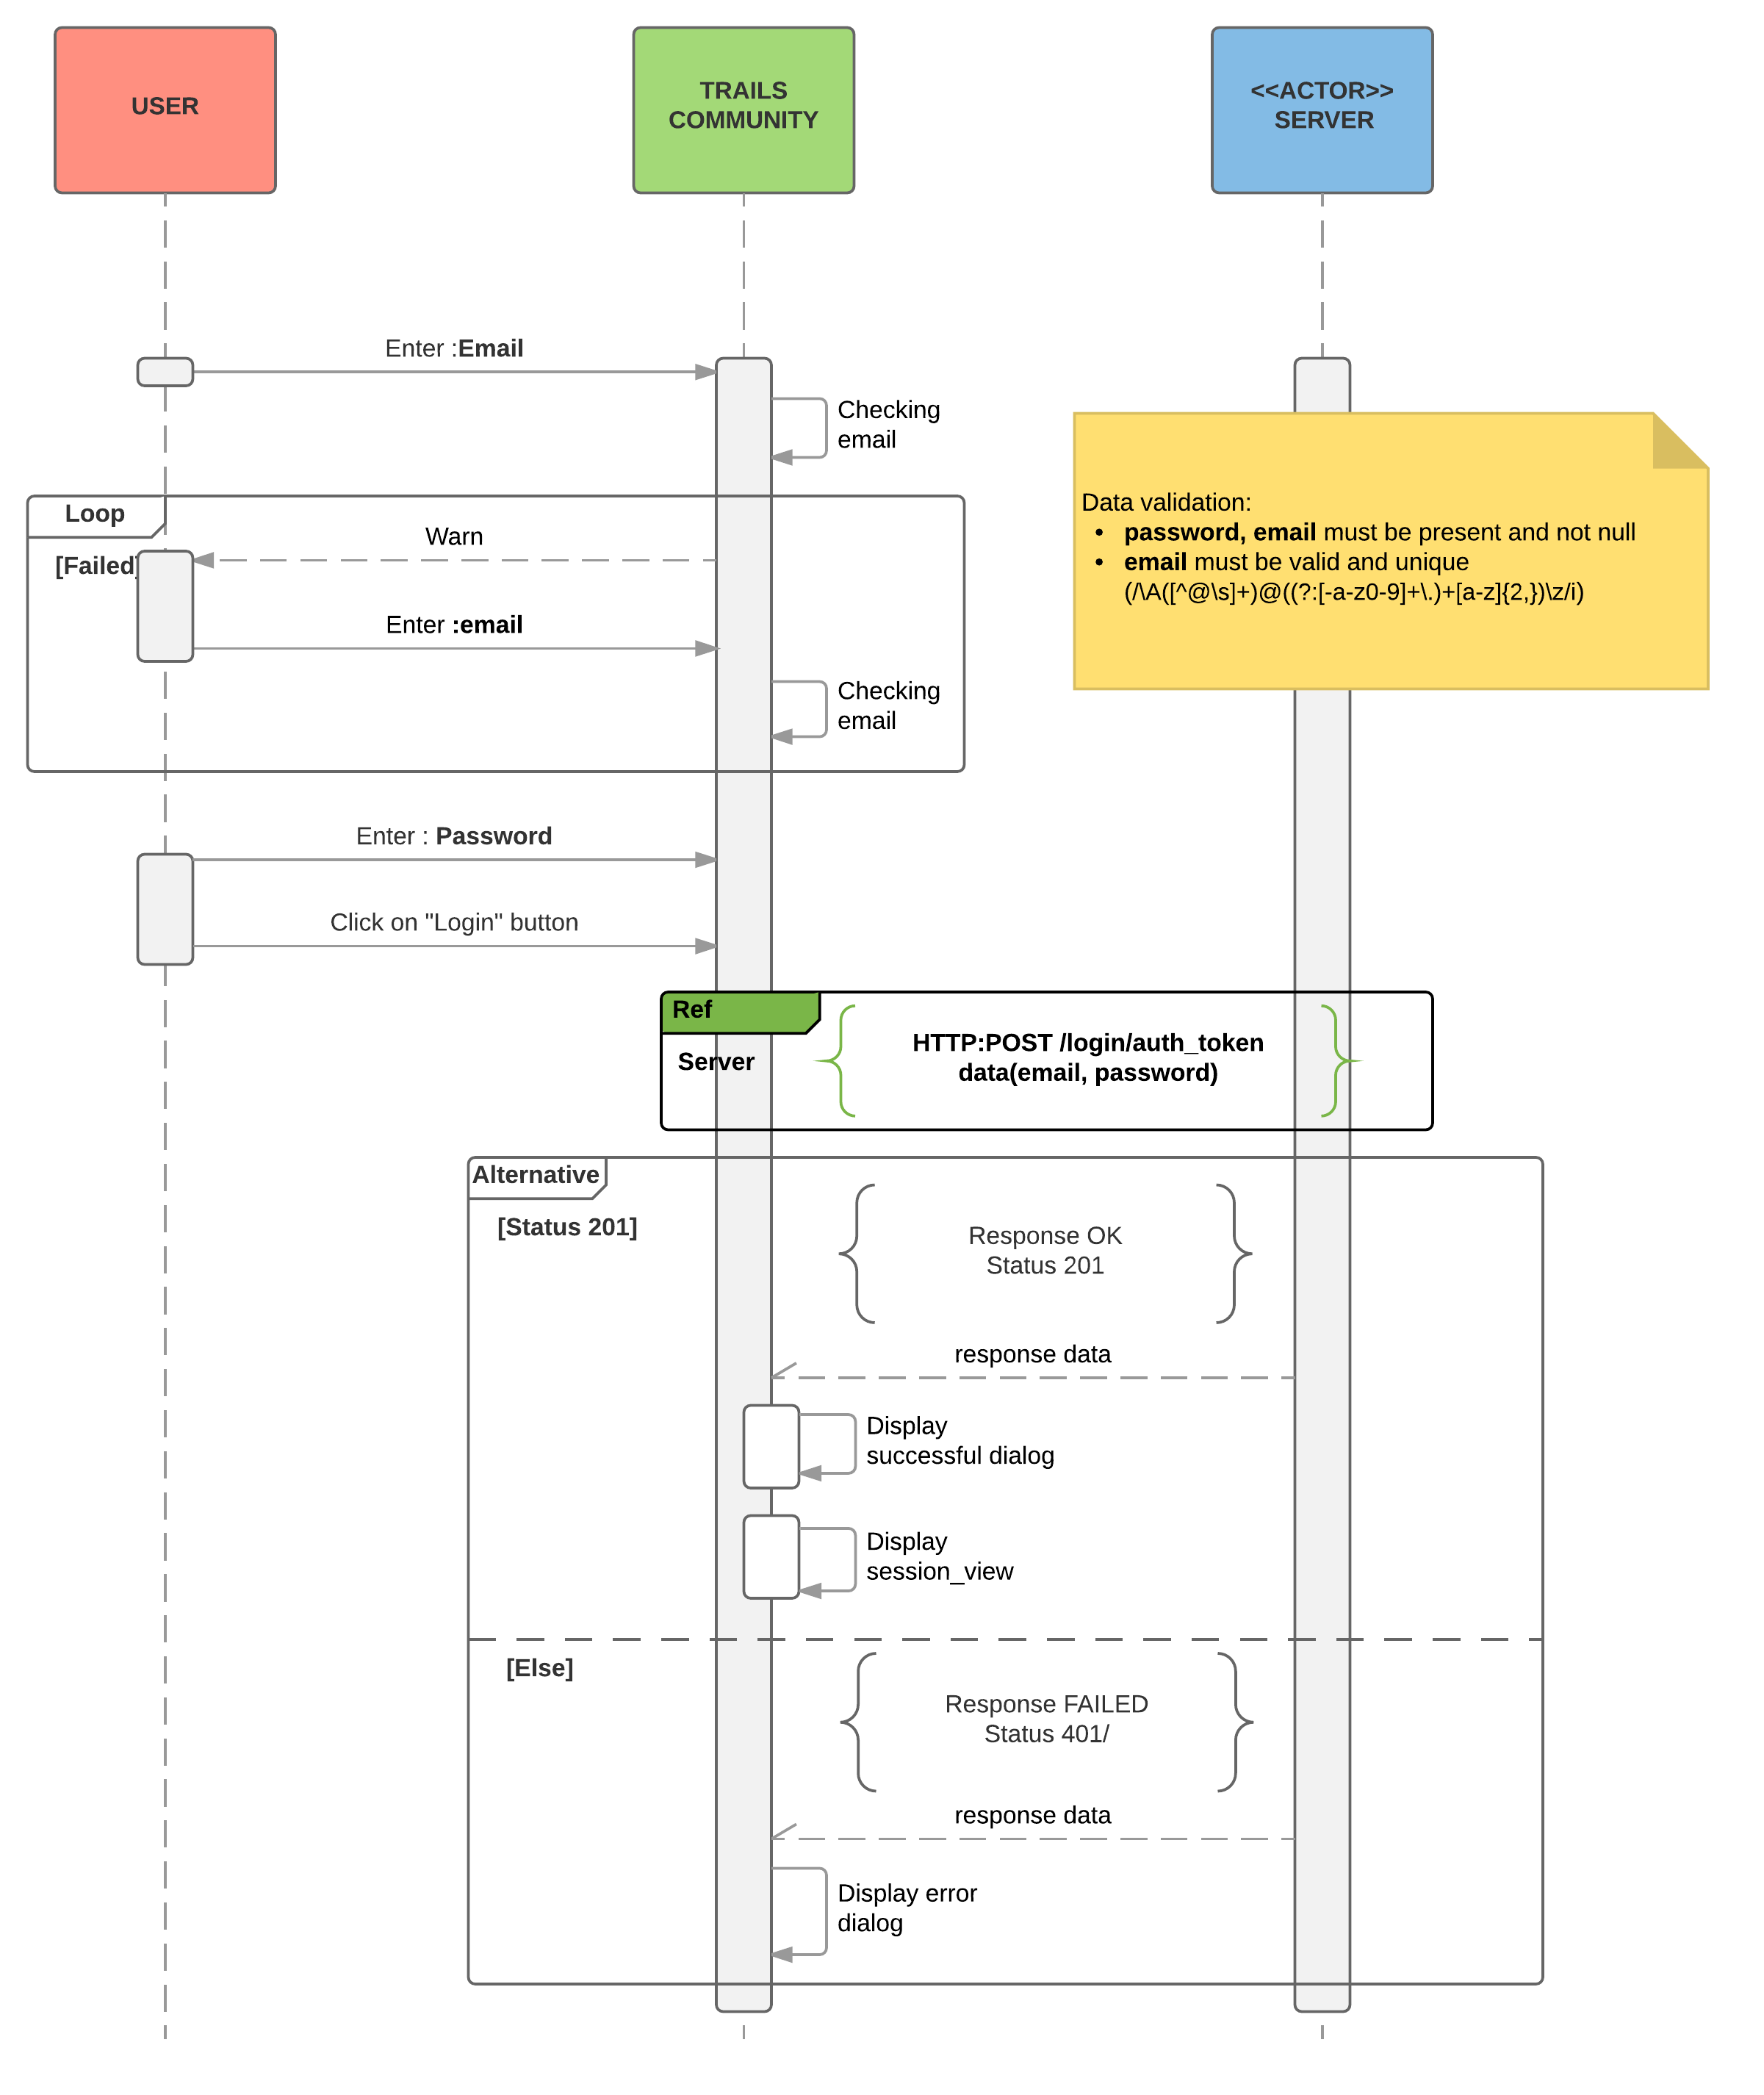
\includegraphics[scale=0.7]{Images/diagram/login_sequence_diagram.png}
\end{figure}

Avant sa première connexion, l'utilisateur devra créer un compte pour obtenir ses informations de connexion. Cette étape est primordiale car certaines données sont sensible. Elle seront utilisés directement par l'application comme le pseudonyme ou le numéro de téléphone.

%Diagramme de séquence créer un compte utilisateur%

\begin{figure}[!h]
	\caption{Diagramme de séquence créer un compte utilisateur}
	\label{register_sequence_diagram}
	\centering
	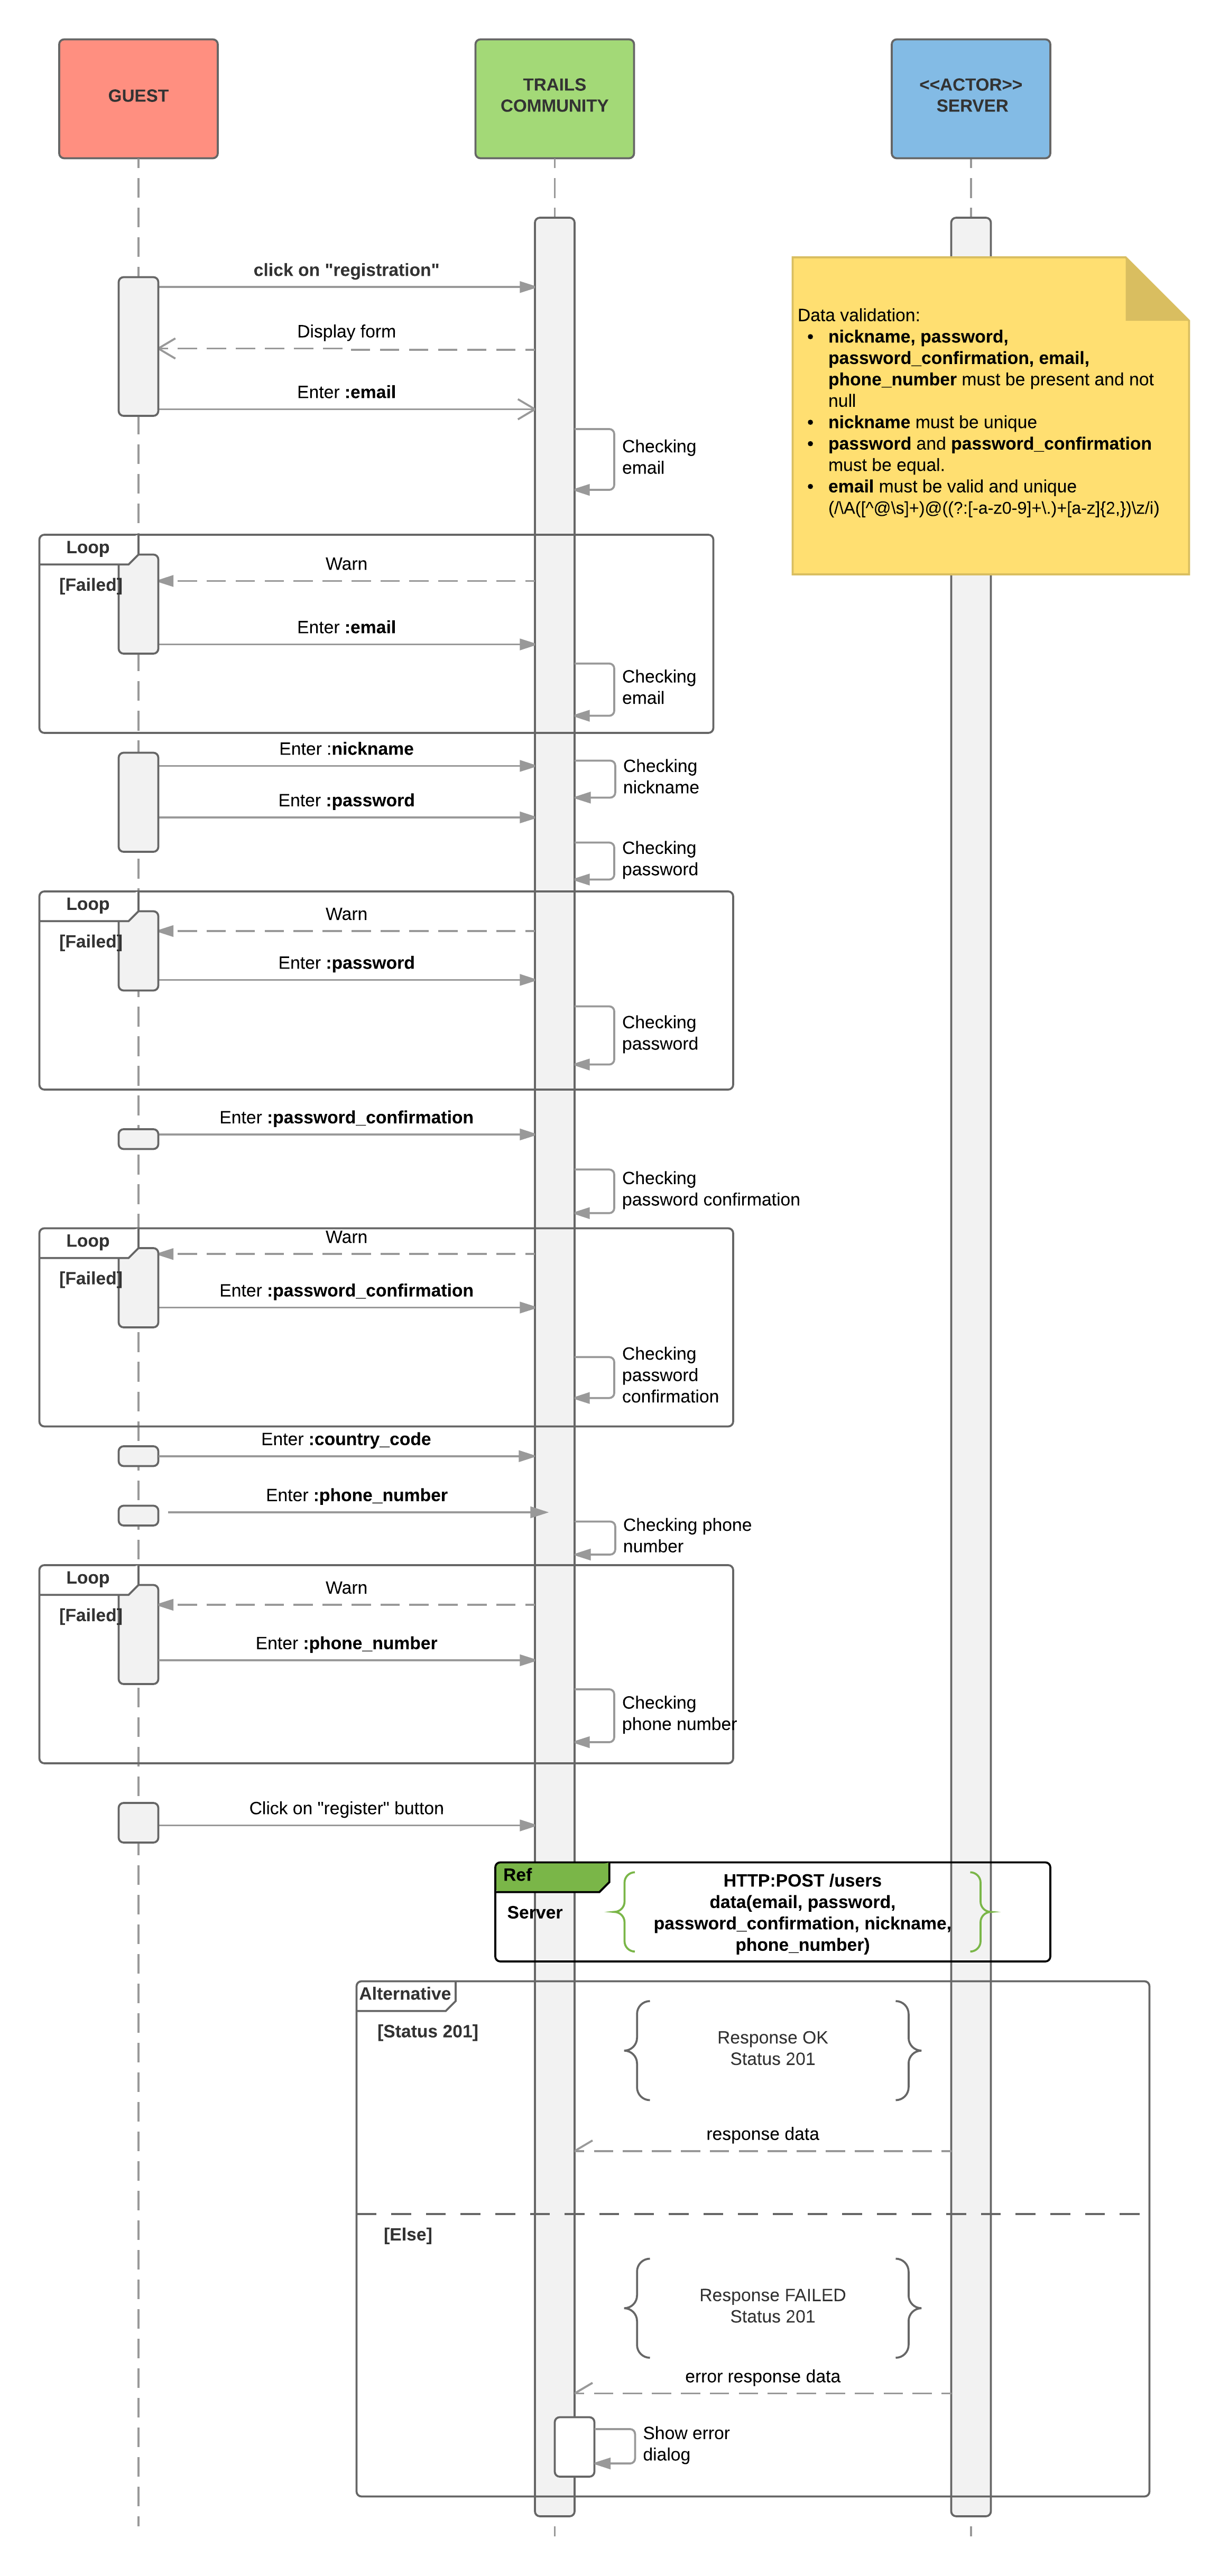
\includegraphics[scale=0.12]{Images/diagram/registration_sequence_diagram.png}
\end{figure}

\clearpage

\subsection{Traitement d'un cas d'utilisation - Créer une session}

\paragraph{}Le cas d'utilisation que nous avons choisi de détailler ici est la création d'une session. C'est un des cas d'utilisation essentiel au fonctionnement de notre application mobile. Sans cette étape, il est impossible de réaliser n'importe quelles actions concrètes sur l'application.
\paragraph{}Le diagramme de séquence s'articule principalement autour de trois étapes : l'authentification, la saisie des données du sondage puis l'envoi des données au serveur.

%Diagramme de séquence créer une session%

\begin{figure}[!h]
	\caption{Diagramme de séquence créer une session}
	\label{create_session_sequence_diagram}
	\centering
	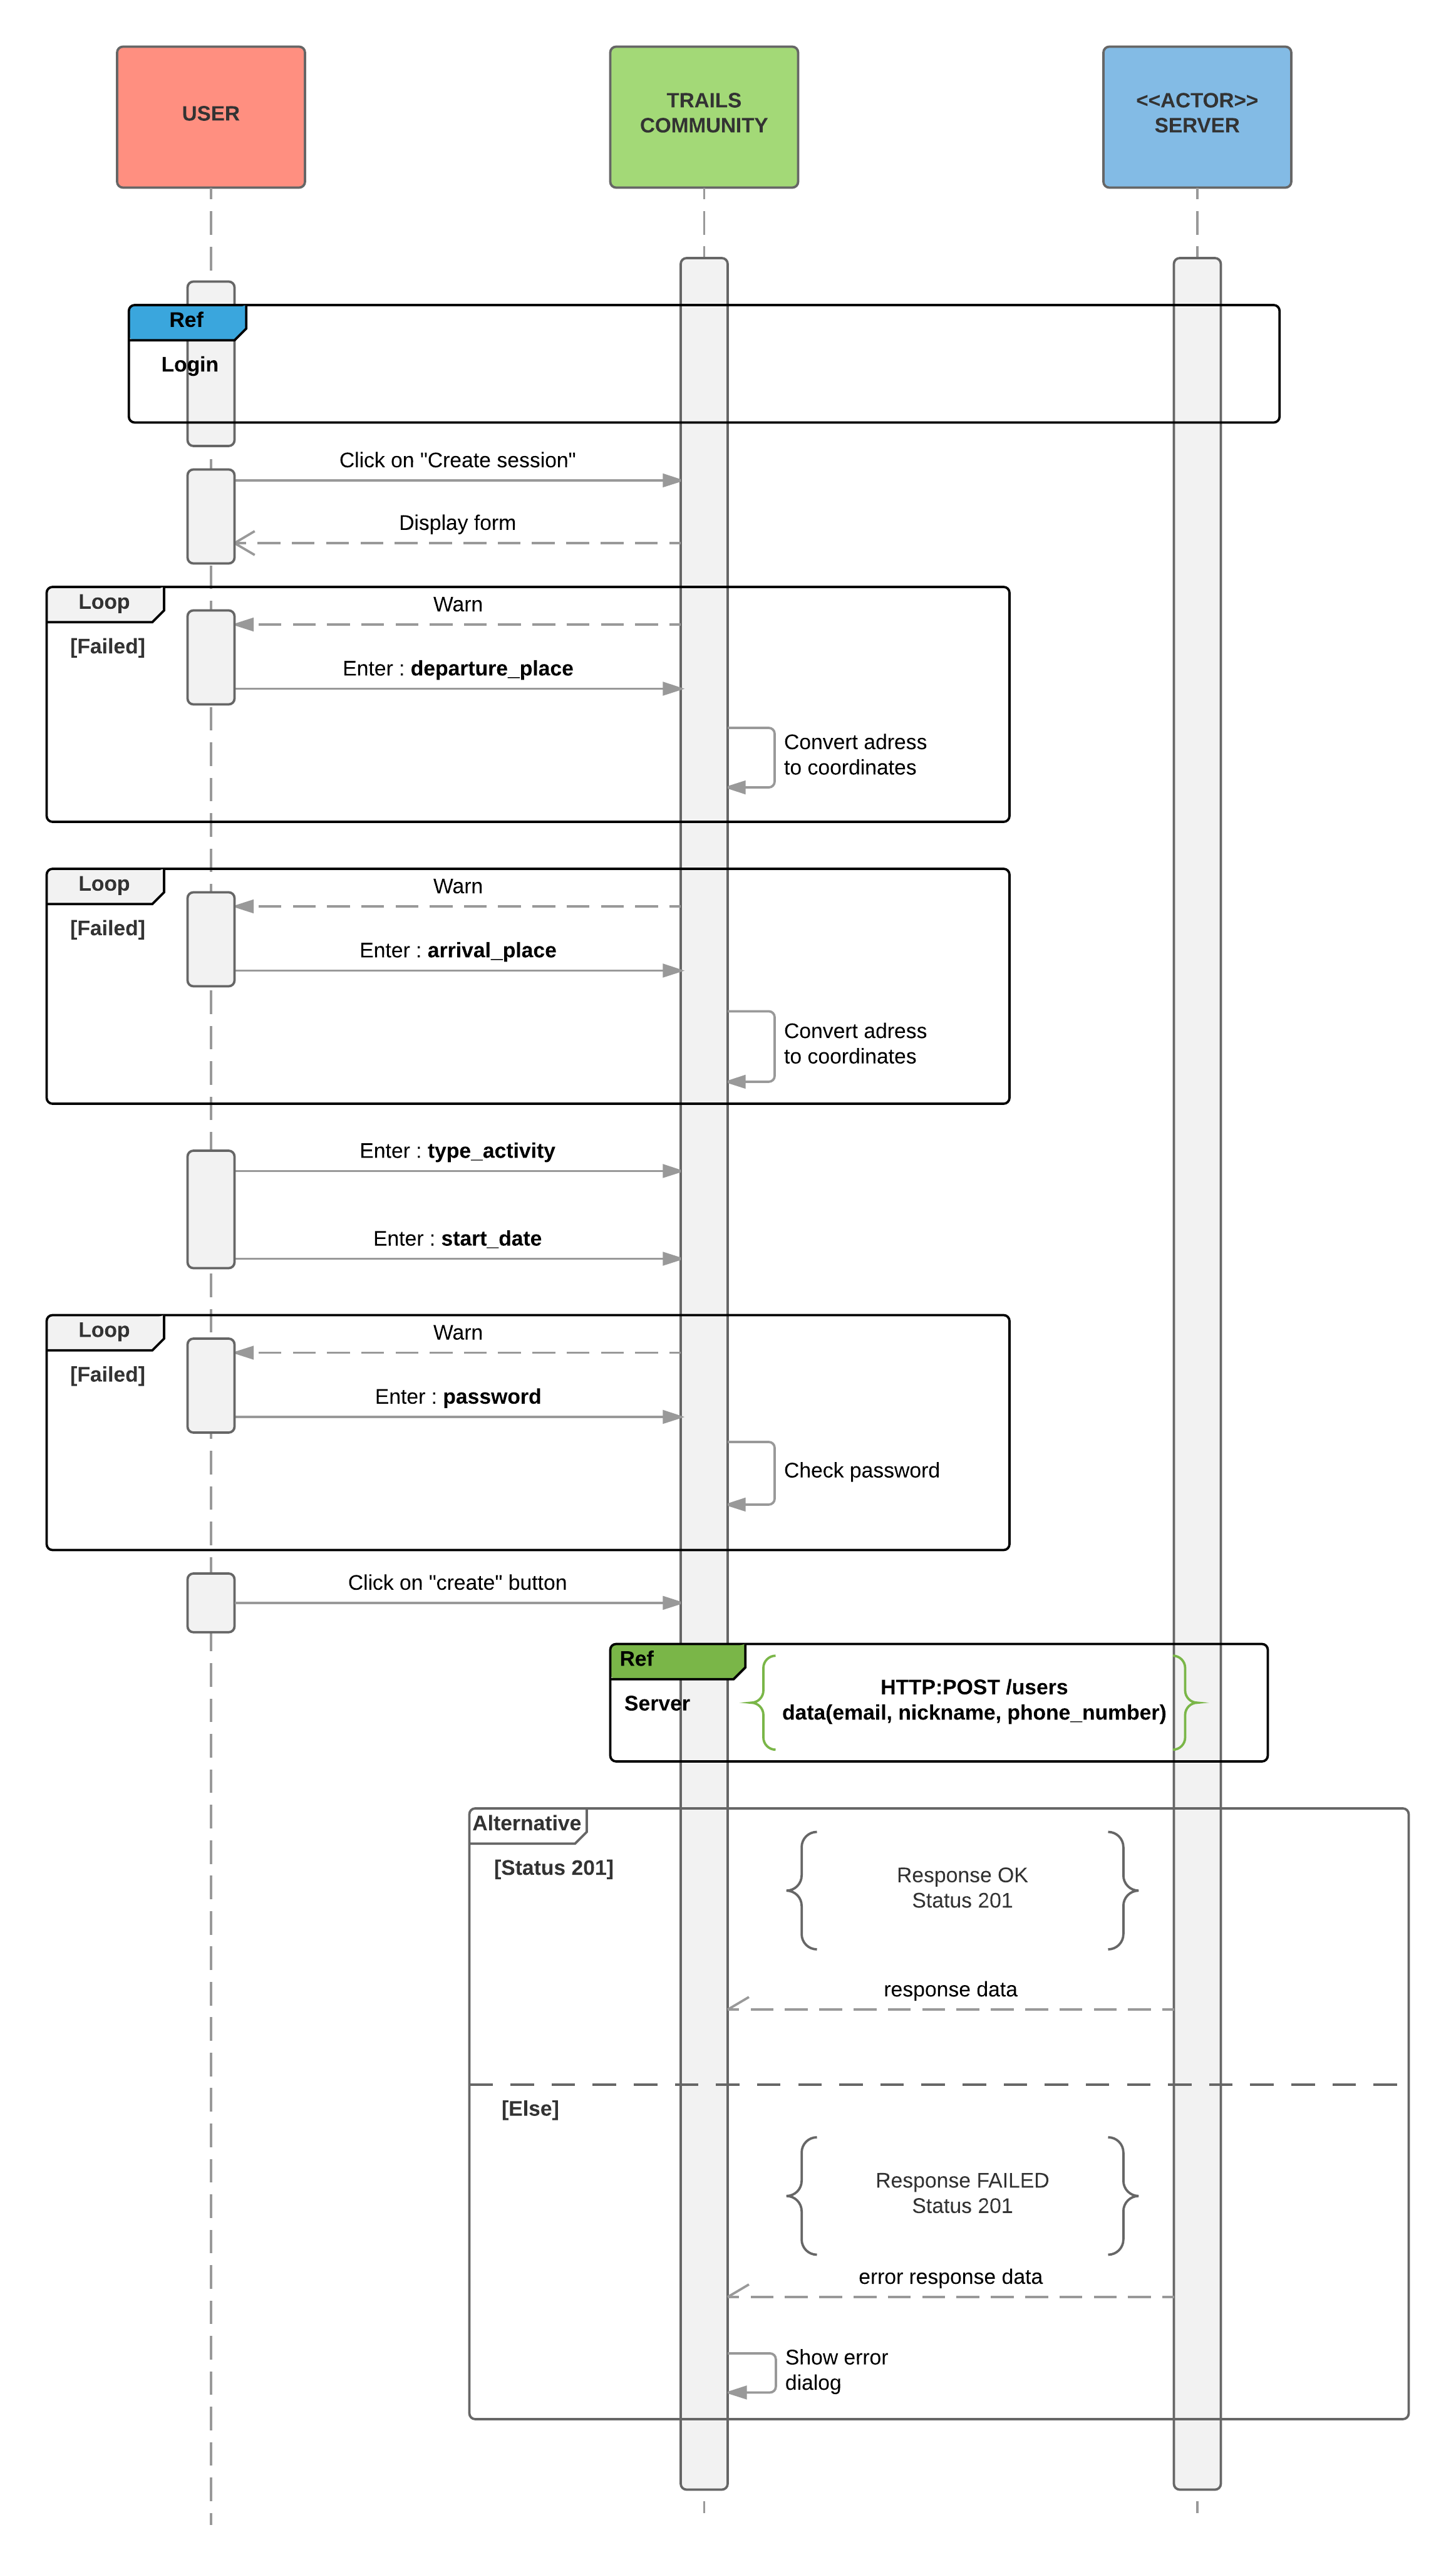
\includegraphics[scale=0.5]{Images/diagram/create_session_sequence_diagram.png}
\end{figure}

\paragraph{}Comme on peut le voir sur le diagramme d'activité. La gestion d'erreur ce passe sur les 2 applications : le client et le serveur. De plus, le serveur se charge de remonter les erreurs sur le format des données ou la lecture/écriture en base de données. Le client informe l'utilisateur sur l'échec du format des données entré en paramètre et aussi l'échec des opération serveur.

%Diagramme d'activité créer une session%

\begin{figure}[!h]
	\caption{Diagramme d'activité de la création d'une session}
	\label{create_session_activity_diagram}
	\centering
	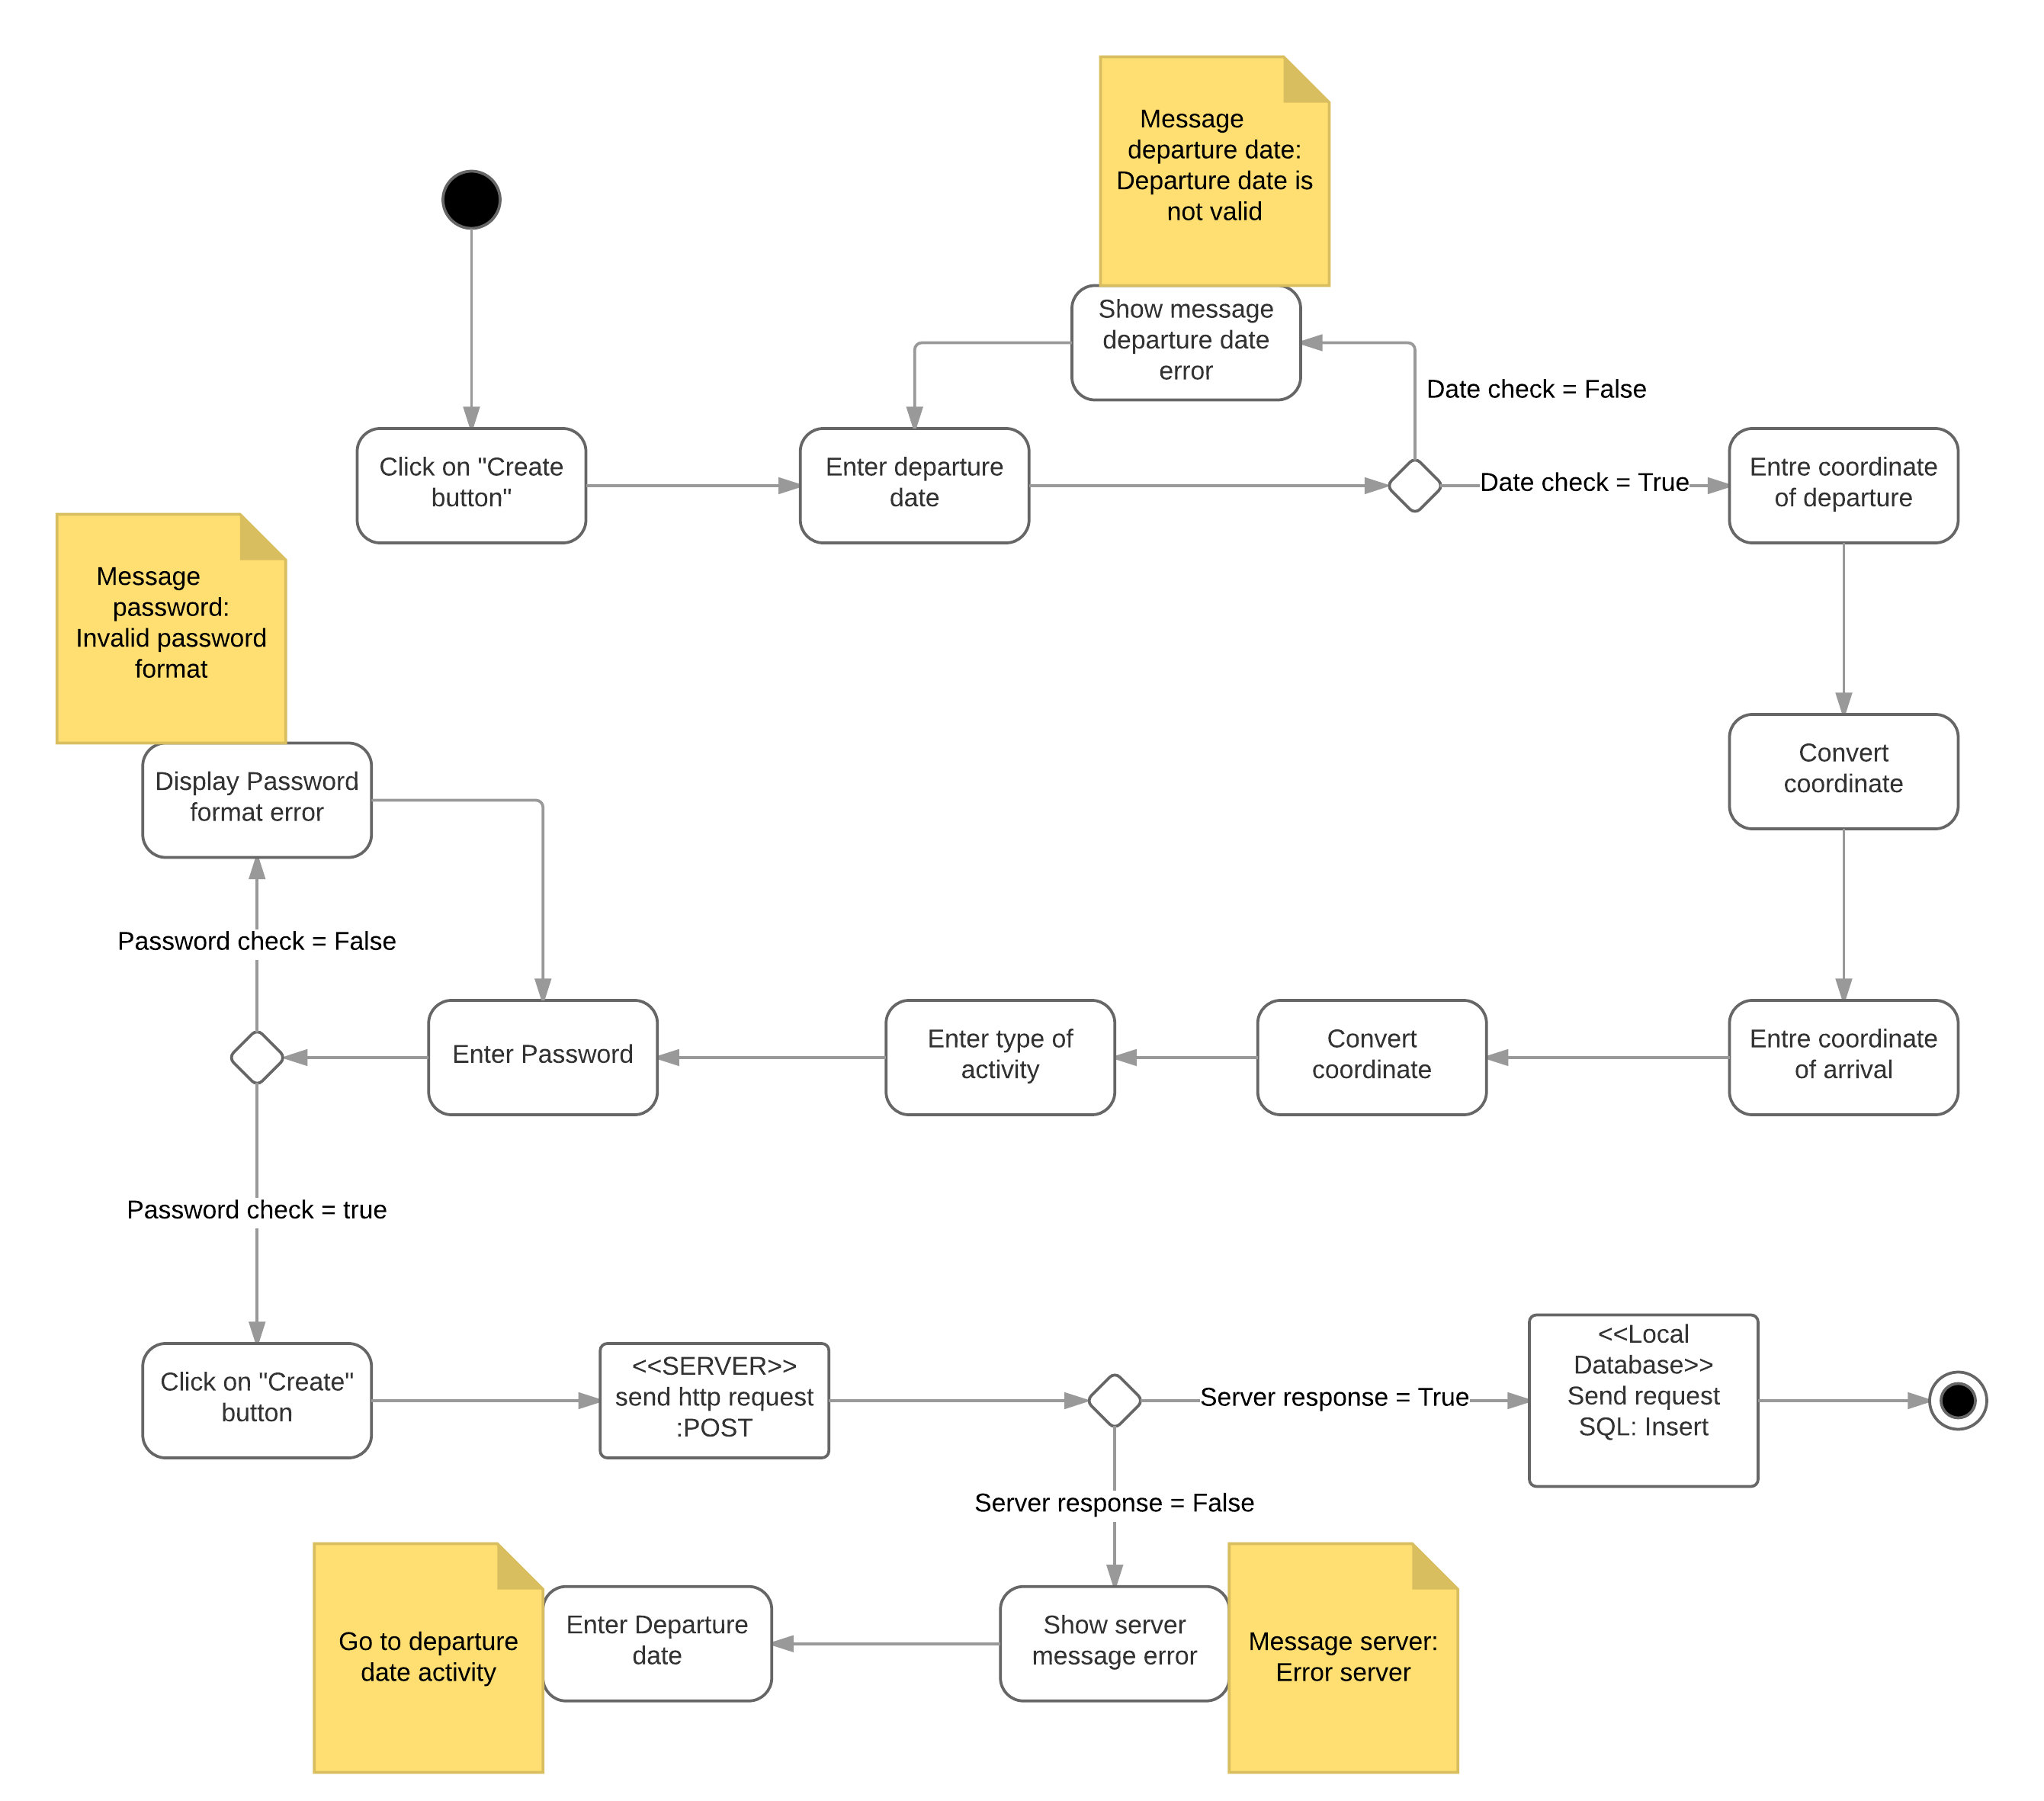
\includegraphics[scale=0.5]{Images/diagram/create_session_activity_diagram.png}
\end{figure}

\subsection{Traitement d'un cas d'utilisation - Rejoindre une session}

\clearpage

%Diagramme de sequence rejoindre une session%

\begin{figure}[!h]
	\caption{Diagramme de séquence rejoindre une session}
	\label{join_session_sequence_diagram}
	\centering
	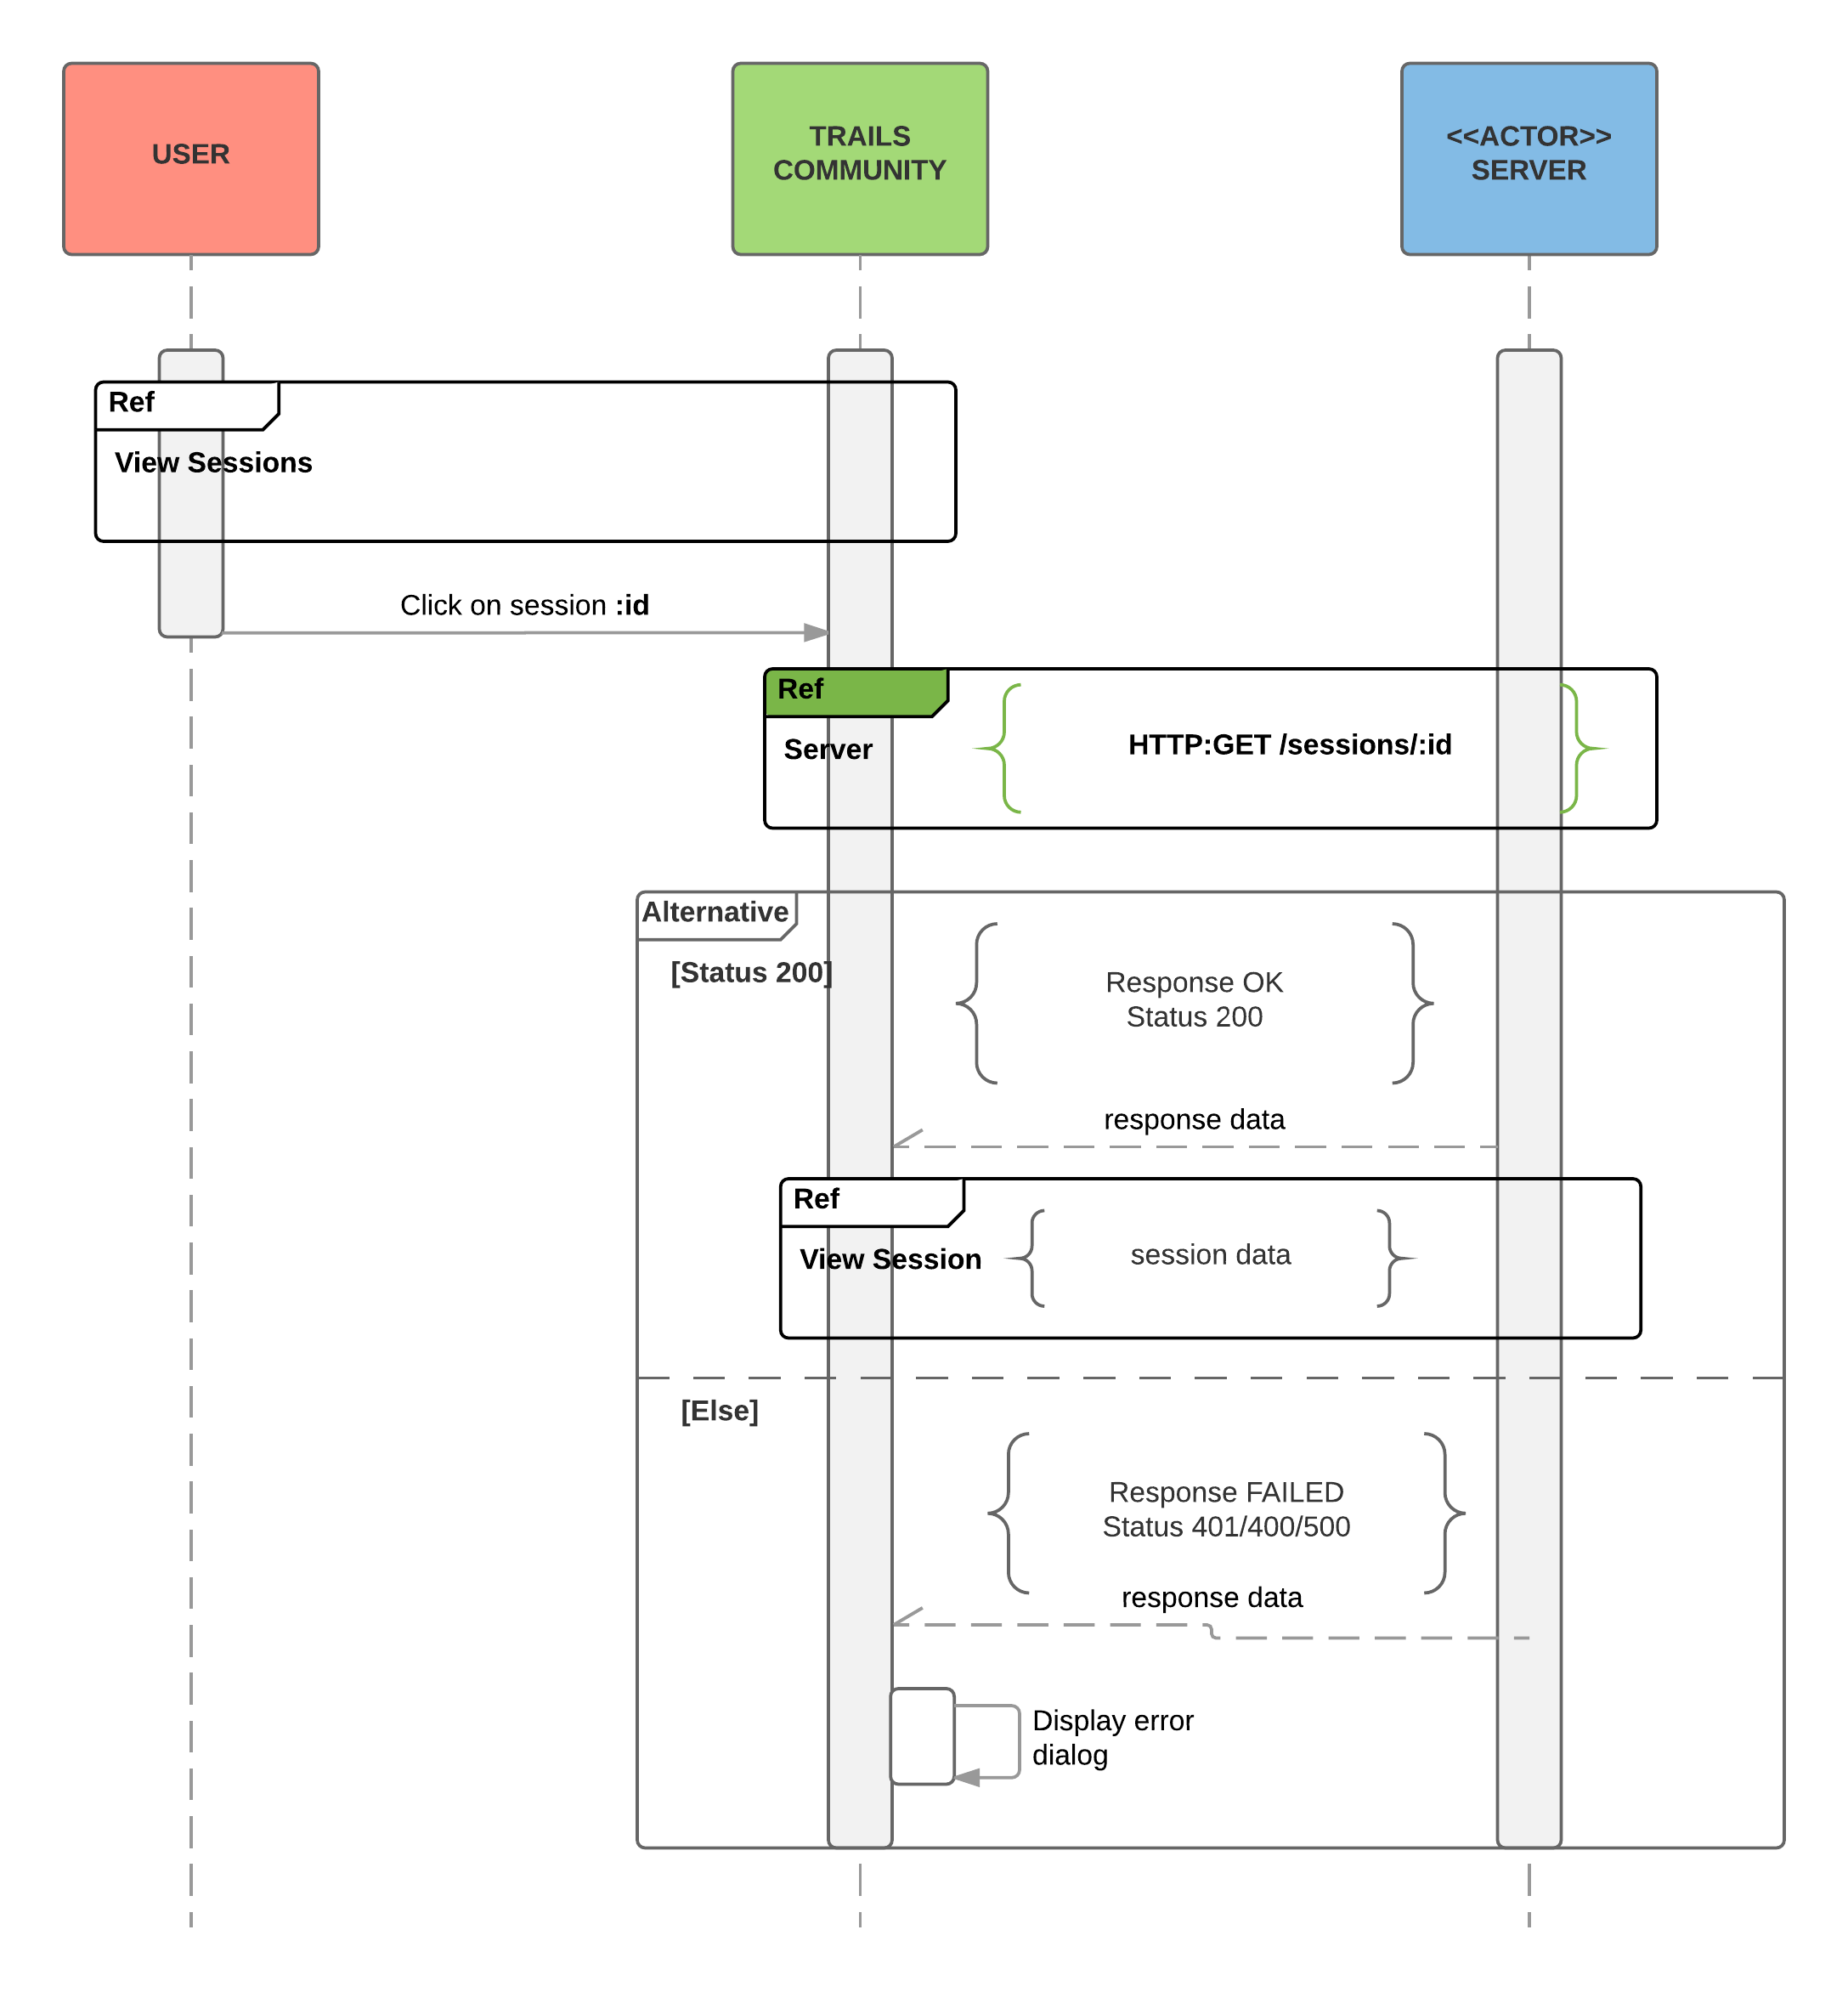
\includegraphics[scale=0.7]{Images/diagram/selection_session_sequence_diagram.png}
\end{figure}

\clearpage

%Diagramme d'activite rejoindre une session%

\begin{figure}[!h]
	\caption{Diagramme d'activité rejoindre une session}
	\label{join_session_activity_diagram}
	\centering
	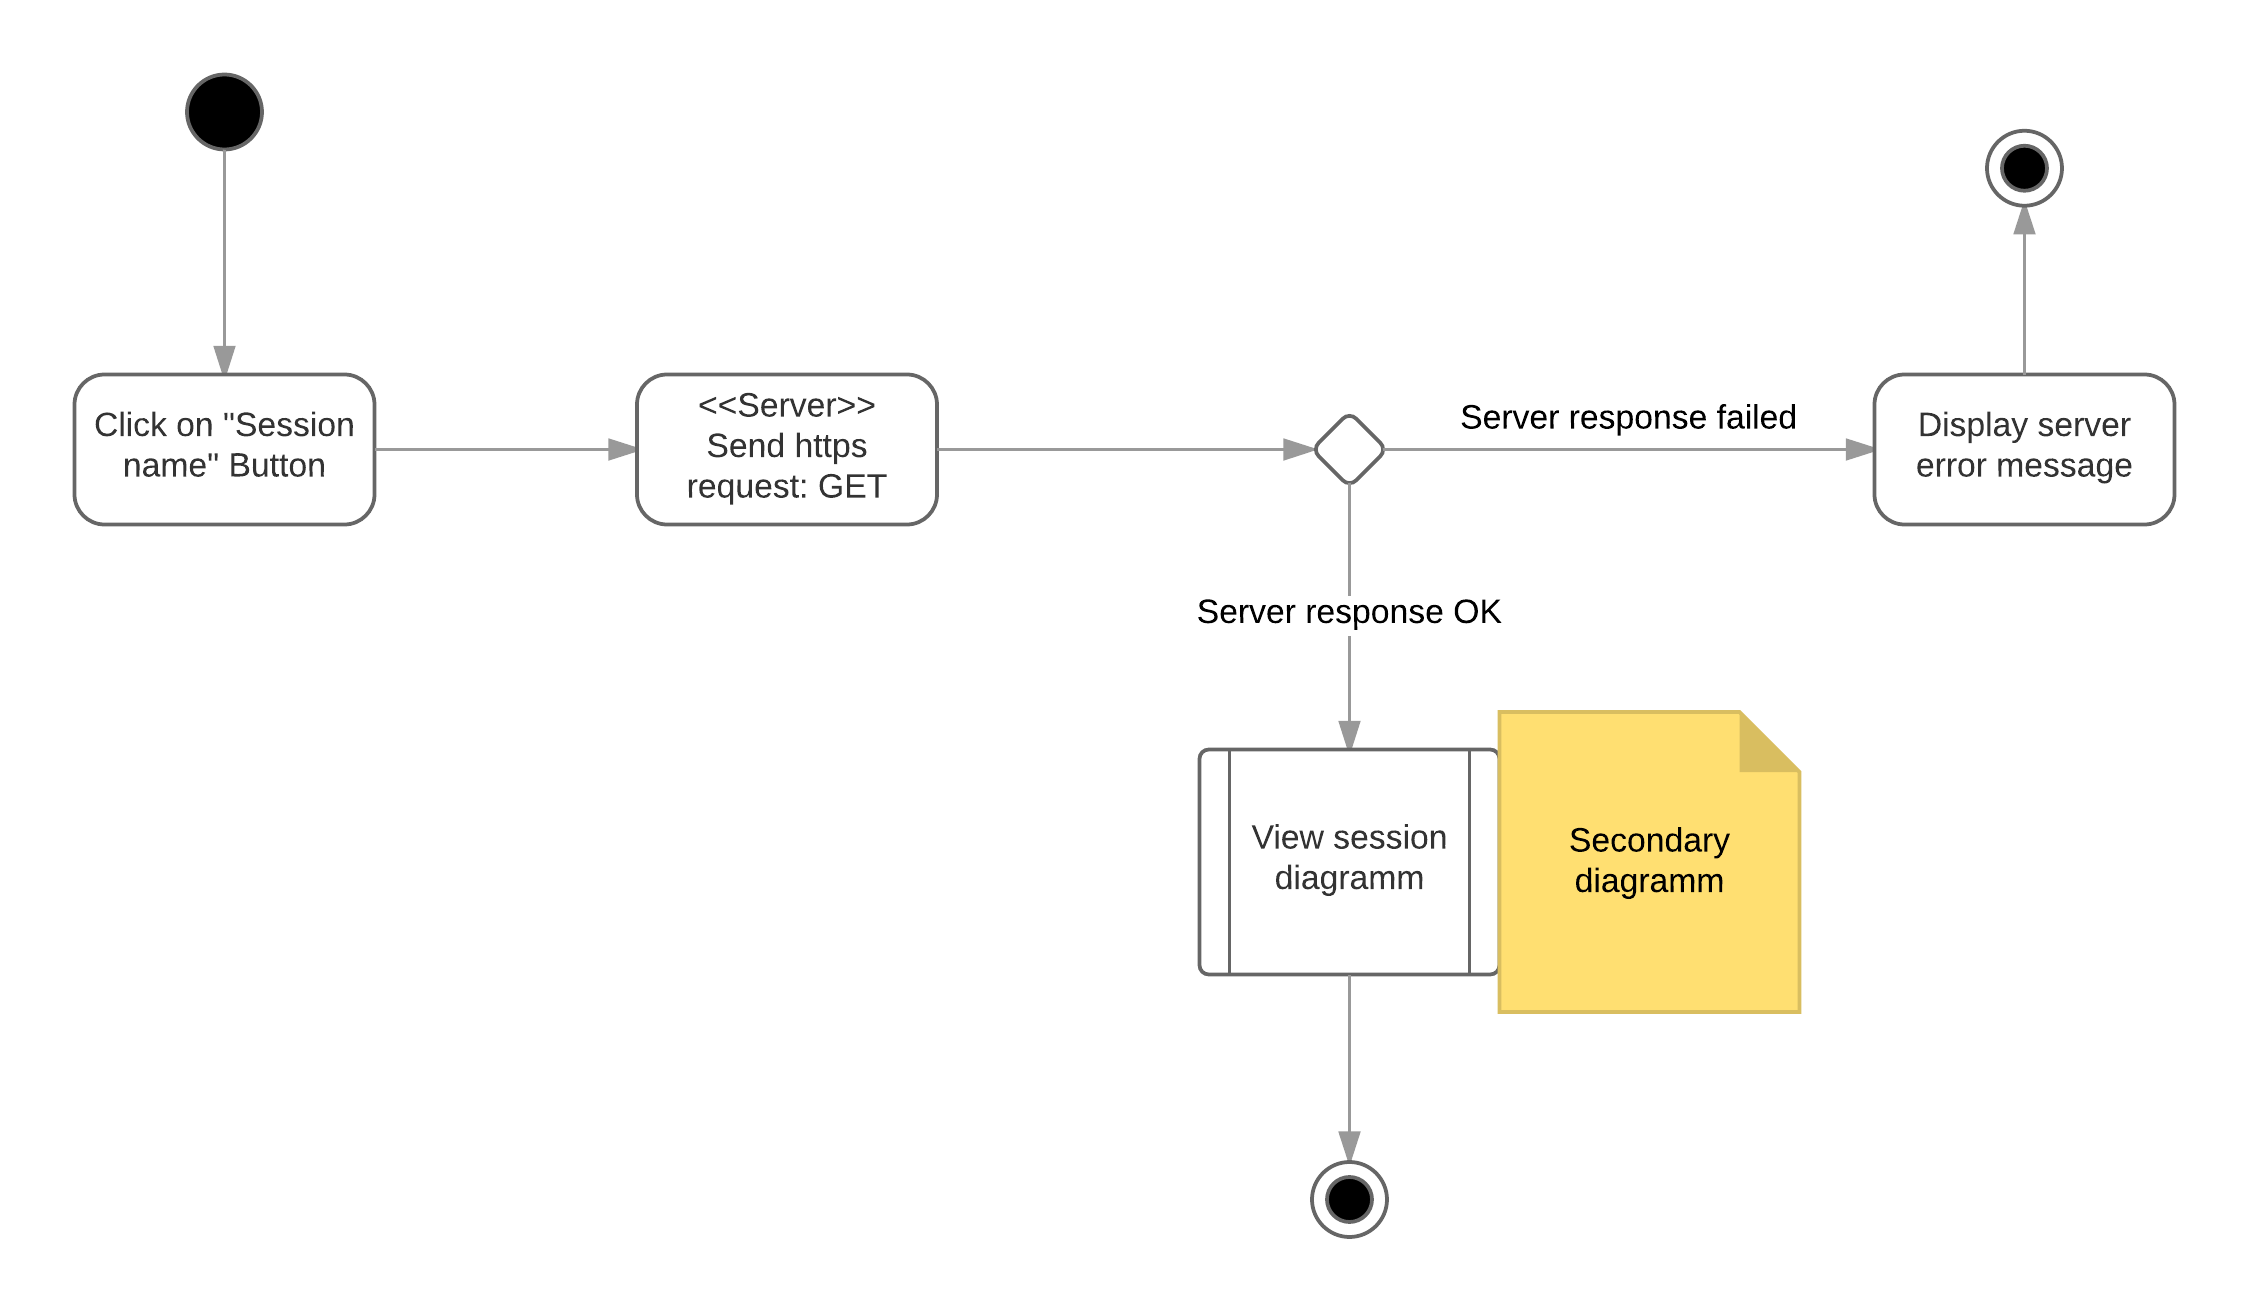
\includegraphics[scale=0.7]{Images/diagram/selection_session_activity_diagram.png}
\end{figure}

\clearpage

%Diagramme d'activite de l'affichage d'une session%

\begin{figure}[!h]
	\caption{Diagramme de séquence de l'affichage d'une session}
	\label{view_session_sequence_diagram}
	\centering
	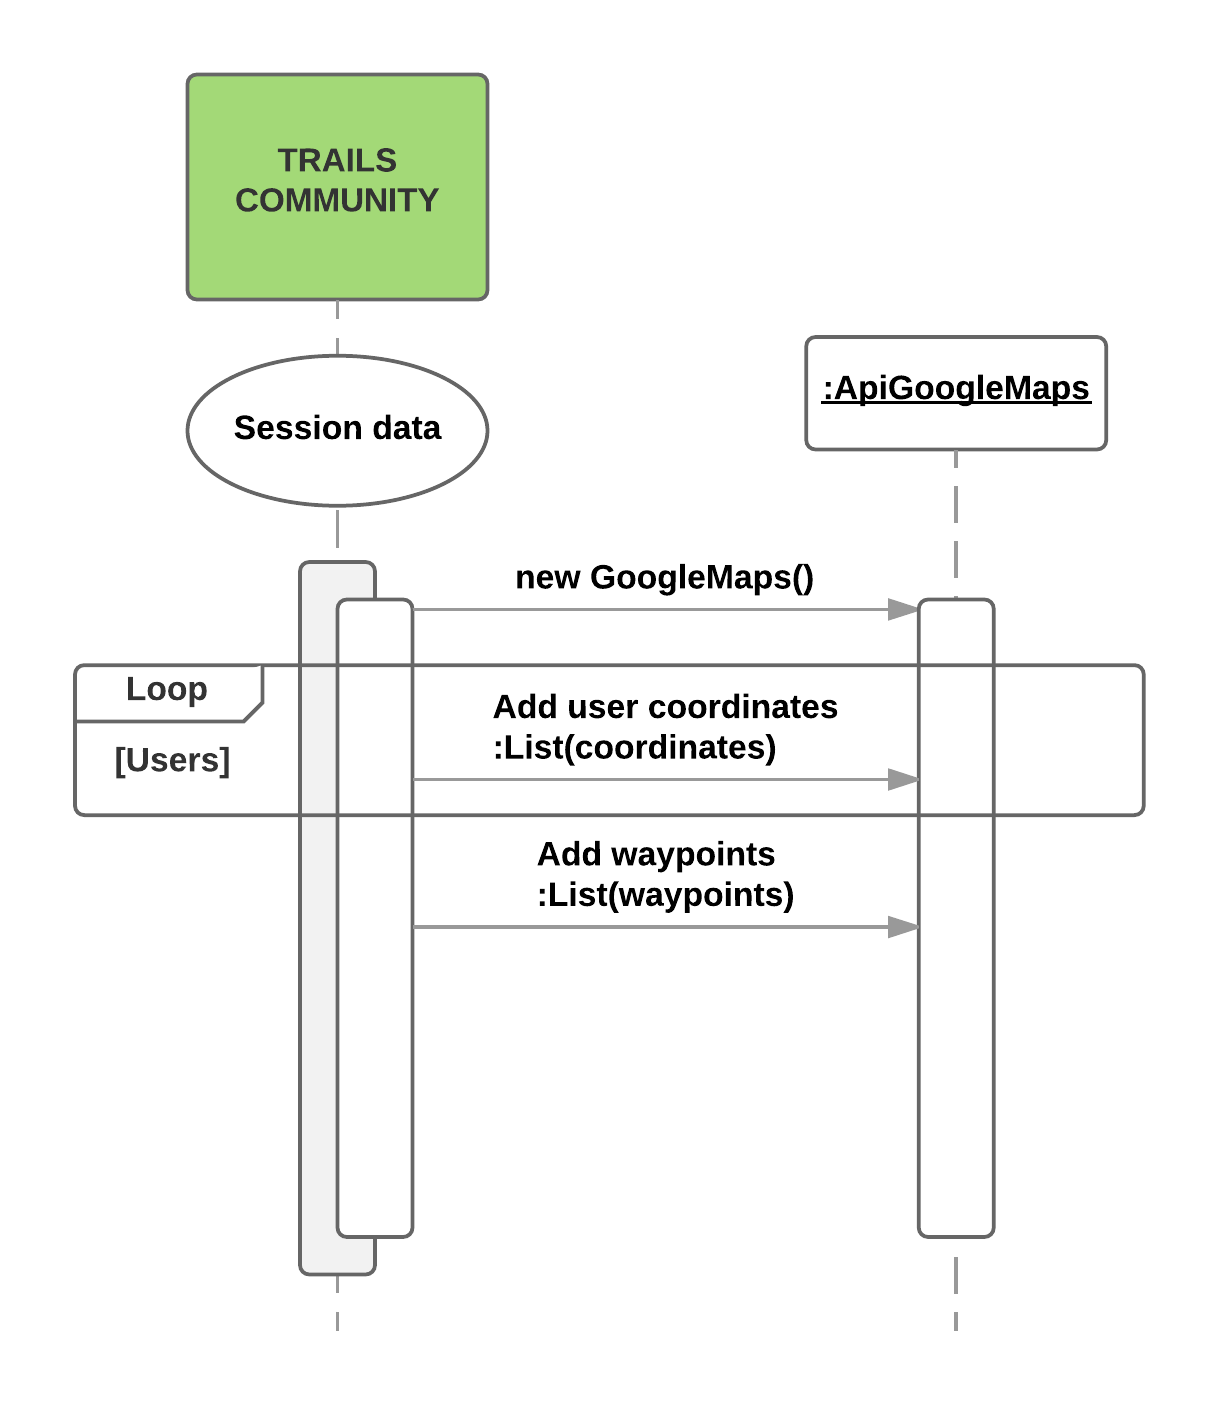
\includegraphics[scale=0.7]{Images/diagram/view_session_sequence_diagram.png}
\end{figure}

\clearpage

\begin{figure}[!h]
	\caption{Diagramme d'activité de l'affichage d'une session}
	\label{view_session_activity_diagram}
	\centering
	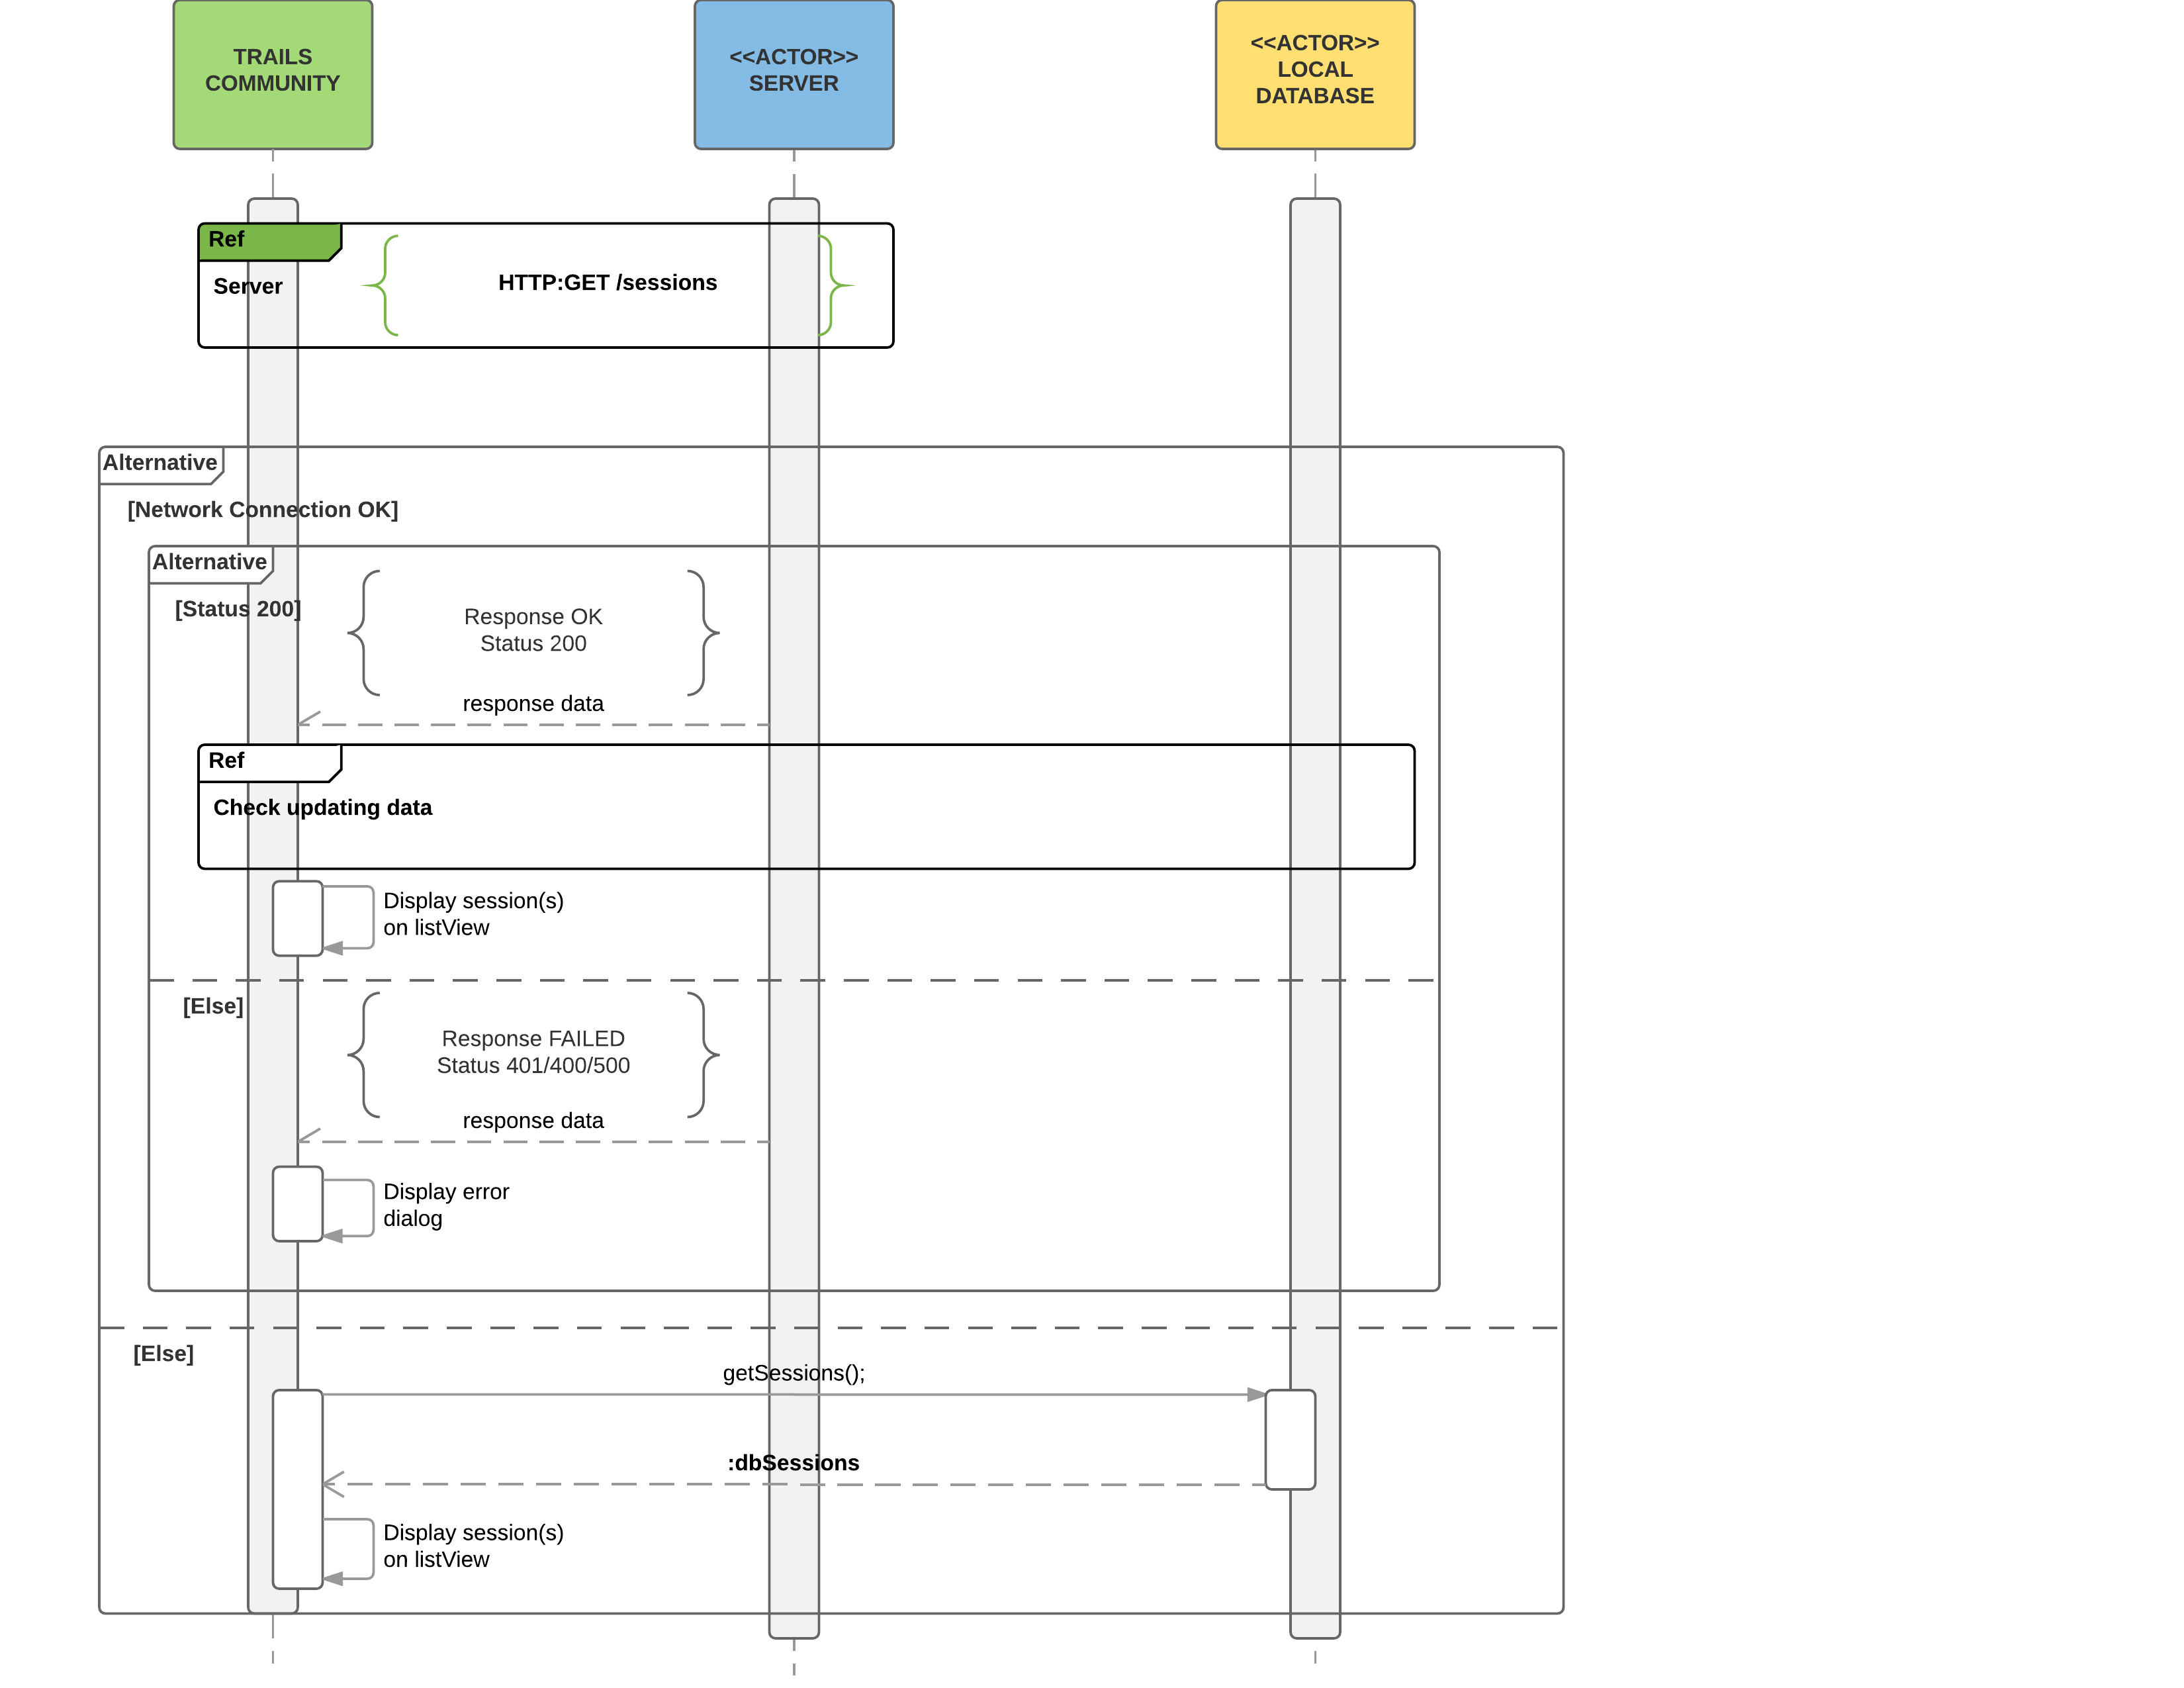
\includegraphics[scale=0.2]{Images/diagram/view_session_activity_diagram.png}
\end{figure}

\clearpage

%Test client%

\section{Test}

\paragraph{}L'ensemble des fonctionnalités de l'application seront tester avec un panel de test important. Du côté du client, des test unitaire ainsi que des tests graphiques seront réalisé pour tester la robusté de l'application et son bon comportement.

\subsection{Test unitaire}

\begin{table}[ht]
\begin{tabularx}{\textwidth}{|X|X|X|}
	\hline
	Identifiant & Titre & Description \\
	\hline
	1 & JSON session valide & Test la conversion d'un JSON en objet Session \\
	\hline
	2 & Parse date invalide & Teste la conversion d'un JSON non valide, c'est à dire qui ne possède pas de date en objet Session \\
	\hline
	3 & JSON session invalide & Teste la conversion du JSON en objet Session \\
	\hline
	4 & Teste la validité d'un email & Teste via une regex si un email est valide ou non \\
	\hline
	5 & Teste la non validité d'un email & Teste un tableau d'emails non valide \\
	\hline \hline
\end{tabularx}
\end{table}

\subsection{Test UI}

\begin{table}[ht]
\begin{tabularx}{\textwidth}{|X|X|X|}
	\hline
	Identifiant & Titre & Description \\
	\hline
	1 & Teste tout les champs de la vue LoginActivity & Entre pour chaque champs une donnée valide pour tester l'authentification d'un utilisateur \\
	\hline
	2 & Teste si le champs email est valide de la vue LoginActivity & Entre un email pour teste si la validation de l'email fonctionne \\	
	\hline
	3 & Teste l'affichage d'erreur sur le champs email de la vue LoginActivity & Entre un email invalide pour tester l'affichage de l'erreur \\
	\hline
	4 & Teste le champs mot de passe de la vue LoginActivity & Entre un mot de passe non valide pour tester l'affichage de l'erreur \\
	\hline
	5 & Teste si une erreur s'affiche lorsque le mot de passe est vide dans la vue LoginActivity & Entre un mot de passe vide pour tester l'affichage de l'erreur \\
	\hline
	6 & Teste tout les champs de la vue SingupActivity & Entre pour chaque champs une données valide pour tester la création d'un compte utilisateur \\
	\hline
	7 & Teste l'affichage d'erreur pour le champs mot de passe de la vue SingupActivity & Entre un mot de passe vide pour tester l'affichage d'erreur du mot de passe vide \\
	\hline
	8 & Teste si la forme de l'email est valide de la vue SingupActivity & Entre un email invalide pour tester l'affichage d'erreur de l'email invalide  \\
	\hline
	9 & Teste si les 2 mots de passe sont valide de la vue SingupActivity & Entre 2 mots de passe différent pour tester l'affichage d'erreur lorsque les mots de passe sont différents \\
	\hline
	10 & Teste le cas d'erreur d'un mot de passe vide de la vue SingupActivity & Entre un mot de passe vide pour afficher le cas d'erreur  \\
	\hline
	11 & Teste le cas d'erreur d'un pseudonyme vide de la vue SingupActivity & Entre un champs vide pour le pseudonyme pour tester l'affichage du cas d'erreur \\
	\hline
	12 & Teste le cas d'erreur d'un numéro de téléphone vide de la vue SingupActivity & Entre un champs vide pour le numéro de téléphone pour tester l'affichage du cas d'erreur  \\
	\hline
	13 & Teste l'ajout d'un waypoint de la vue SessionActivity & Ajoute un waypoint sur la Google maps  \\
	\hline
	14 & Teste l'action du bouton chat de la vue SessionActivity & Teste si le chat s'affiche bien lors du clique de l'utilisateur sur le bouton chat  \\
	\hline \hline
\end{tabularx}
\end{table}

\begin{table}[ht]
\begin{tabularx}{\textwidth}{|X|X|X|}
\hline
15 & Teste l'ajout d'un message dans le chat de la vue SessionActivity & Ajoute un message dans le chat pour tester son affichage et son ajout dans la liste du chat  \\
\hline
16 & Teste le cas d'erreur dans un message vide dans le chat de la vue SessionActivity & Ajoute un message vide dans le chat pour tester l'affichage du cas d'erreur  \\
\hline
17 & Teste la fermeture du chat de la vue SessionActivity & Teste si le chat se ferme bien lors du clique de l'utilisateur sur le bouton chat  \\
\hline
18 & Teste la conversion d'une adresse en coordonnées GPS dans la vue SessionFormActivity & Teste la conversion d'une adresse en coordonnées GPS  \\
\hline
19 & Teste la création d'une session de la vue SessionFormActivity & Ajout dans chaque champs de la vue une entrée valide pour tester la création d'une session  \\
\hline
20 & Teste l'affichage d'erreur du champs lieu de départ de la vue SessionFormActivity & Teste pour le champs lieu de départ si l'affichage du cas d'erreur fonctionne si le champs est vide \\
\hline
21 & Teste l'affichage d'erreur du champs lieu de d'arrivé de la vue SessionFormActivity & Teste pour le champs lieu de d'arrivé si l'affichage du cas d'erreur fonctionne si le champs est vide \\
\hline
22 & Teste l'affichage d'erreur du champs date de départ de la vue SessionFormActivity & Teste pour le champs date de départ si l'affichage du cas d'erreur fonctionne si le champs est vide \\
\hline
23 & Teste l'affichage d'erreur du champs mot de passe de la vue SessionFormActivity & Teste pour le champs  si l'affichage du cas d'erreur fonctionne si le champs est vide \\
\hline \hline
\end{tabularx}
\end{table}


\part{Serveur TrailsCommunity}

\chapter{Introduction}

\section{Conventions}
\begin{itemize}
	\item \textbf{Client} : Application client.
	\item \textbf{Statut} : Code réponse de la requête HTTP
	\item Toutes les réponses possibles sont listés sous la catégorie 'Réponse'
	\item Toutes les réponses sont du format JSON
\end{itemize}


\section{Codes statut}

\paragraph{} Tous les codes de statut sont des standards HTTP. Cette API utilisera les suivants : 
\begin{itemize}
	\item $ 2XX $ - Succès de la requête
	\item $ 4XX $ - Erreur du côté client
	\item $ 5XX $ - Erreur du côté serveur		
\end{itemize}

\paragraph{}

\begin{center}
	\begin{tabular}{|c|c|}
		\hline
		Code statut & Description \\
		\hline \hline
		$ 200 $ & Requête traitée avec succès \\
		\hline 
		$ 201 $ & Requête traitée avec succès et création d'un document \\	
		\hline 
		$ 202 $ & Requête traitée avec succès mais pas d'information à renvoyer \\
		\hline \hline 
		$ 400 $ & La syntaxe de la requête est erronée \\	
		\hline 
		$ 401 $ & Une authentification est nécessaire pour accéder à la ressource \\	
		\hline
		$ 404 $ & Ressource non trouvée \\
		\hline \hline
		$ 500 $ & Erreur interne du serveur \\
		\hline
		$ 503 $ & Service temporairement indisponible ou en maintenance \\ 	
		\hline
	\end{tabular}
\end{center}

\chapter{Ressources}

%
% Authentification
%
\section{Authentification}
\subsection{Requête}

\begin{center}
	\begin{tabular}{|c|c|}
		\hline
		Méthode & URL \\
		\hline
		$ POST $ 
		&
		\begin{lstlisting}
api/login/auth_token
		\end{lstlisting} 
		\\ \hline
	\end{tabular}
\end{center}


\begin{center}
	\begin{tabular}{|c|c|c|}
		\hline
		Type & Paramètres & Valeurs \\
		\hline
		$ HEADER $ & 
		\begin{lstlisting}
Application/json
		\end{lstlisting} &
		$ String $ \\ \hline
		$ JSON $ & 
		\begin{lstlisting}
{
	"auth": {
		"email": "mail@mail.com",
		"password": "FZ,f235nDE",
	}
}
		\end{lstlisting} & \makecell{$ String $ \\ $ String $} \\
		\hline
		
	\end{tabular}
\end{center}

\par $ email $ : correspond à l'adresse mail valide de l'utilisateur
\par $ password $ : mot de passe de l'utilisateur

\subsection{Réponse}

\begin{center}
	\begin{tabular}{|c|c|}
		\hline
		Statut & Réponse \\
		\hline
		$ 200 $ & \begin{lstlisting}
{ "jwt": <Authorization> }
		\end{lstlisting} \\ 
		\hline
		$ 401 $ & \\
		\hline
		$ 500 $ & \\
		\hline
	\end{tabular}
\end{center}

\par $ Authorization ( string ) $ - Tous les autres appels nécessitant une
authentification doivent avoir cette clé dans le header.

%
% Inscription
%

\section{Inscription}

\subsection{Requête}

\paragraph{} Enregistrement d'un utilisateur dans le système.

\begin{center}
	\begin{tabular}{|c|c|}
	\hline
	Méthode & URL \\
	\hline
	$ POST $ 
	&
	\begin{lstlisting}
api/users/
	\end{lstlisting} 
	\\ \hline
	\end{tabular}
\end{center}


\begin{center}
	\begin{tabular}{|c|c|c|}
	\hline
	Type & Paramètres & Valeurs \\
	\hline
	$ HEADER $ & 
	\begin{lstlisting}
Application/json
	\end{lstlisting} &
	$ String $ \\ \hline
	$ JSON $ & 
	\begin{lstlisting}
{
	"nickname": "Arthur83",
	"email": "apaul@custom.com",
	"phone_number": "+33651678908",
	"password": "myPassword33",
	"password_confirmation": "myPassword33"
}
	\end{lstlisting} & \makecell{$ String $ \\ $ String $ \\ $ String $ \\ $ String $ \\ $ String $} \\ 
	\hline
	
	\end{tabular}
\end{center}

\par $ nickname $ : pseudonyme de l'utilisateur
\par $ email $ : email de l'utilisateur non nul et valide
\par $ password $ : mot de passe d'utilisateur
\par $ password_confirmation $ : confirmation du mot de passe de l'utilisateur. Il doit être identique à $ password $.

\subsection{Réponse}

\begin{center}
	\begin{tabular}{|c|c|}
		\hline
		Statut & Réponse \\
		\hline
		$ 201 $ & \begin{lstlisting}
{
  "data": {
    "id": 2,
    "nickname": "Arthur83",
    "phone_number": "+33651678908",
    "current_session_id": null
  }
}
\end{lstlisting} \\ 
\hline
$ 400 $ & \begin{lstlisting}
{
  "errors": {
    "nickname": [
      "has already been taken"
    ],
    "email": [
      "is invalid"
    ]
  }
}
		\end{lstlisting} \\
		\hline
		$ 500 $ & \\
		\hline
	\end{tabular}
\end{center}

%
% Ajout d'une session
%

\section{Ajout d'une session}

\subsection{Requête}

\paragraph{} Permet d'ajouter une nouvelle session dans le serveur. Cette ressource est contrainte d'un token d'authentification <$Authorization$> qui a été donnée avec la ressource $api/login/auth\_token$

\begin{center}
	\begin{tabular}{|c|c|}
	\hline
	Méthode & URL \\
	\hline
	$ POST $ 
	&
	\begin{lstlisting}
api/sessions/
	\end{lstlisting} 
	\\ \hline
	\end{tabular}
\end{center}


\begin{center}
	\begin{tabular}{|c|c|c|}
	\hline
	Type & Paramètres & Valeurs \\
	\hline
	$ HEADER $ & 
	\begin{lstlisting}
Application/json
	\end{lstlisting} &
	$ String $ \\ \hline
	$ HEADER $ & 
	\begin{lstlisting}
Authorization
	\end{lstlisting} &
	$ String $ \\ \hline
	$ JSON $ & 
	\begin{lstlisting}
{
	"activity": 1,
	"password": "lockSessionPsw",
	"departure_place": "43.179363;5.717782",
	"arrival_place": "43.191168;5.730819",
	"start_date": "2016-11-20"
}
	\end{lstlisting} & \makecell{$ Integer $ \\ $ String $ \\ $ String $ \\ $ String $ \\ $ Date $} \\ 
	\hline
	
	\end{tabular}
\end{center}

\par $ activity $ : identifiant de l'activité. (1: randonnée, 2: vélo, ...)
\par $ password $ : mot de passe de la session, permet de restreindre l'entrée.
\par $ departure\_place $ : lieu de départ. Couple de position géographique $(latitude;longitude)$
\par $ arrival\_place $ : lieu d'arrivée. Couple de position géographique $(latitude;longitude)$

\subsection{Réponse}

\begin{center}
	\begin{tabular}{|c|c|}
		\hline
		Statut & Réponse \\
		\hline
		$ 200 $ & \begin{lstlisting}
{
  "data": {
    "id": 5,
    "activity": 1,
    "departure_place": "43.179363;5.717782",
    "arrival_place": "43.191168;5.730819",
    "start_date": "2016-11-20",
    "close": false,
    "lock": true,
    "user": {
      "id": 1,
      "nickname": "Raptor234",
      "phone_number": "+33623569450",
      "current_session_id": null
    },
    "coordinates": [],
    "waypoints": []
  }
}
		\end{lstlisting} \\ 
		\hline
		$ 400 $ & \begin{lstlisting}
{
  "errors": {
    "activity": [
      "can't be blank",
      "is not a number"
    ]
  }
}
		\end{lstlisting} \\
		\hline
		$ 401 $ & \\
		\hline
		$ 500 $ & \\
		\hline
	\end{tabular}
\end{center}

%
% Liste des session
%

\section{Liste des sessions}

\subsection{Requête}

\paragraph{} Permet de récupérer la liste des sessions du système. Cette ressource est contrainte d'un token d'authentification <$Authorization$> qui a été donnée avec la ressource $api/login/auth\_token$

\begin{center}
	\begin{tabular}{|c|c|}
	\hline
	Méthode & URL \\
	\hline
	$ GET $ 
	&
	\begin{lstlisting}
api/sessions/
	\end{lstlisting} 
	\\ \hline
	\end{tabular}
\end{center}


\begin{center}
	\begin{tabular}{|c|c|c|}
	\hline
	Type & Paramètres & Valeurs \\
	\hline
	$ HEADER $ & 
	\begin{lstlisting}
Authorization
	\end{lstlisting} &
	$ String $ \\ \hline
	
	\end{tabular}
\end{center}

\subsection{Réponse}

\begin{center}
	\begin{tabular}{|c|c|}
		\hline
		Statut & Réponse \\
		\hline
		$ 200 $ & \begin{lstlisting}
{
  "data": [
    {
      "id": 1,
      "activity": 1,
      "departure_place": "43.179363;5.717782",
      "arrival_place": "43.191168;5.730819",
      "start_date": "2016-11-20",
      "close": false,
      "lock": true,
      "user": {
        "id": 2,
        "nickname": "Arthur83",
        "phone_number": "+33651678908",
        "current_session_id": null
      }
    },
    {
      "id": 2,
      "activity": 3,
      "departure_place": "43.179363;5.717782",
      "arrival_place": "43.191168;5.730819",
      "start_date": "2016-11-20",
      "close": false,
      "lock": true,
      "user": {
        "id": 2,
        "nickname": "Arthur83",
        "phone_number": "+33651678908",
        "current_session_id": null
      }
    }
  ]
}
		\end{lstlisting} \\ 
		\hline
		$ 401 $ & \\
		\hline
		$ 500 $ & \\
		\hline
	\end{tabular}
\end{center}

%
% Session Get :id
%

\section{Session}

\subsection{Requête}

\paragraph{} Permet de récupérer une session spécifique selon son identifiant (ID). Cette ressource est contrainte d'un token d'authentification <$Authorization$> qui a été donnée avec la ressource $api/login/auth\_token$

\begin{center}
	\begin{tabular}{|c|c|}
	\hline
	Méthode & URL \\
	\hline
	$ GET $ 
	&
	\begin{lstlisting}
api/sessions/:id
	\end{lstlisting} 
	\\ \hline
	\end{tabular}
\end{center}


\begin{center}
	\begin{tabular}{|c|c|c|}
	\hline
	Type & Paramètres & Valeurs \\ \hline
	$ URL\_PARAM $ & 
	\begin{lstlisting}
id
	\end{lstlisting} &
	$ Integer $ \\ \hline
	$ HEADER $ & 
	\begin{lstlisting}
Authorization
	\end{lstlisting} &
	$ String $ \\ \hline
	
	\end{tabular}
\end{center}

\par $ id $ : identifiant de la session voulu
\subsection{Réponse}

\begin{center}
	\begin{tabular}{|c|c|}
		\hline
		Statut & Réponse \\
		\hline
		$ 200 $ & \begin{lstlisting}
{
  "data": {
    "id": 2,
    "activity": 3,
    "departure_place": "43.179363;5.717782",
    "arrival_place": "43.191168;5.730819",
    "start_date": "2016-11-20",
    "close": false,
    "lock": true,
    "user": {
      "id": 2,
      "nickname": "Arthur83",
      "phone_number": "+33651678908",
      "current_session_id": null
    },
    "coordinates": [
      {
        "latitude": 43.179363,
        "longitude": 5.717782,
        "user_id": 1
      }
    ],
    "waypoints": [
      {
        "latitude": 43.179363,
        "longitude": 5.717782
      }
    ]
  }
}
		\end{lstlisting} \\ 
		\hline
		$ 401 $ & \\
		\hline
		$ 404 $ & \begin{lstlisting}
{
  "errors": {
    "session": "Record Not Found"
  }
}
		\end{lstlisting} \\
		\hline
		$ 500 $ & \\
		\hline
	\end{tabular}
\end{center}

%
% Mis à jour d'une session
%

\section{Mis à jour d'une session}

\subsection{Requête}

\paragraph{} Permet de mettre à jour session spécifique selon un identifiant (ID) dans le système. Cette ressource est contrainte d'un token d'authentification <$Authorization$> qui a été donnée avec la ressource $api/login/auth\_token$

\begin{center}
	\begin{tabular}{|c|c|}
	\hline
	Méthode & URL \\
	\hline
	$ PUT $ 
	&
	\begin{lstlisting}
api/sessions/:id
	\end{lstlisting} 
	\\ \hline
	\end{tabular}
\end{center}


\begin{center}
	\begin{tabular}{|c|c|c|}
	\hline
	Type & Paramètres & Valeurs \\
	\hline
	$ HEADER $ & 
	\begin{lstlisting}
Application/json
	\end{lstlisting} &
	$ String $ \\ \hline
	$ HEADER $ & 
	\begin{lstlisting}
Authorization
	\end{lstlisting} &
	$ String $ \\ \hline
	$ JSON $ & 
	\begin{lstlisting}
{
   "close": true
}
	\end{lstlisting} & \makecell{$  boolean $} \\ 
	\hline
	
	\end{tabular}
\end{center}

\par $ close $ : boolean determinant si la session doit être fermée.

\subsection{Réponse}

\begin{center}
	\begin{tabular}{|c|c|}
		\hline
		Statut & Réponse \\
		\hline
		$ 200 $ & \begin{lstlisting}
{
  "data": {
    "id": 7,
    "activity": 3,
    "departure_place": "43.179363;5.717782",
    "arrival_place": "43.191168;5.730819",
    "start_date": "2016-11-20",
    "close": true,
    "lock": true,
    "user": {
      "id": 2,
      "nickname": "Arthur83",
      "phone_number": "+33651678908",
      "current_session_id": 1
    },
    "coordinates": [],
    "waypoints": []
  }
}
		\end{lstlisting} \\ 
		\hline
		$ 401 $ & \\
		\hline
		$ 500 $ & \\
		\hline
	\end{tabular}
\end{center}

%
% Rejoindre une Session
%

\section{Rejoindre une session}

\subsection{Requête}

\paragraph{} Permet de à l'utilisateur de rejoindre une session spécifique selon son identifiant (ID). Cette ressource est contrainte d'un token d'authentification <$Authorization$> qui a été donnée avec la ressource $api/login/auth\_token$. De plus, un mot de passe peut être demandé si la session est restreinte.

\begin{center}
	\begin{tabular}{|c|c|}
	\hline
	Méthode & URL \\
	\hline
	$ GET $ 
	&
	\begin{lstlisting}
api/sessions/:id/join
	\end{lstlisting} 
	\\ \hline
	\end{tabular}
\end{center}


\begin{center}
	\begin{tabular}{|c|c|c|}
	\hline
	Type & Paramètres & Valeurs \\ \hline
	$ HEADER $ & 
	\begin{lstlisting}
Authorization
	\end{lstlisting} &
	$ String $ \\ \hline
	$ URL\_PARAM $ & 
	\begin{lstlisting}
id
	\end{lstlisting} &
	$ Integer $ \\ \hline
	$ URL\_PARAM $ & 
	\begin{lstlisting}
password (optional)
	\end{lstlisting} &
	$ String $ \\ \hline
	\end{tabular}
\end{center}

\par $ id $ : identifiant de la session voulu
\subsection{Réponse}

\begin{center}
	\begin{tabular}{|c|c|}
		\hline
		Statut & Réponse \\
		\hline
		$ 200 $ & \\ 
		\hline
		$ 400 $ & \begin{lstlisting}
{
  "errors": {
    "session": "Bad password." OR
    "session": "This session needs a password to join it."
  }
}
		\end{lstlisting} \\
		\hline
		$ 401 $ & \\
		\hline
		$ 404 $ & \begin{lstlisting}
{
  "errors": {
    "session": "Record Not Found"
  }
}
		\end{lstlisting} \\
		\hline
		$ 500 $ & \\
		\hline
	\end{tabular}
\end{center}

%
% Ajout d'un waypoint
%

\section{Ajout d'un waypoint}

\subsection{Requête}

\paragraph{} Permet de à l'utilisateur d'ajouter une nouveau waypoint pour une session spécifique selon son identifiant (ID). Cette ressource est contrainte d'un token d'authentification <$Authorization$> qui a été donnée avec la ressource $api/login/auth\_token$

\begin{center}
	\begin{tabular}{|c|c|}
	\hline
	Méthode & URL \\
	\hline
	$ POST $ 
	&
	\begin{lstlisting}
api/sessions/:id/waypoint
	\end{lstlisting} 
	\\ \hline
	\end{tabular}
\end{center}


\begin{center}
	\begin{tabular}{|c|c|c|}
	\hline
	Type & Paramètres & Valeurs \\ \hline
	$ URL\_PARAM $ & 
	\begin{lstlisting}
id
	\end{lstlisting} &
	$ Integer $ \\ \hline
	$ HEADER $ & 
	\begin{lstlisting}
Authorization
	\end{lstlisting} &
	$ String $ \\ \hline
	$ JSON $ & 
	\begin{lstlisting}
{
	"latitude": 43.179363,
	"longitude": 5.717782 
}
	\end{lstlisting} & \makecell{$ Double $ \\ $ Double $} \\  \hline
	
	\end{tabular}
\end{center}

\par $ id $ : identifiant de la session voulu
\subsection{Réponse}

\begin{center}
	\begin{tabular}{|c|c|}
		\hline
		Statut & Réponse \\
		\hline
		$ 200 $ & \\ 
		\hline
		$ 401 $ & \\
		\hline
		$ 404 $ & \begin{lstlisting}
{
  "errors": {
    "session": "Record Not Found"
  }
}
		\end{lstlisting} \\
		\hline
		$ 500 $ & \\
		\hline
	\end{tabular}
\end{center} 

\section{Ajout d'une coordonnée}

\subsection{Requête}

\paragraph{} Permet de à l'utilisateur d'ajouter une nouvelle coordonnée pour une session spécifique selon son identifiant (ID). Cette ressource est contrainte d'un token d'authentification <$Authorization$> qui a été donnée avec la ressource $api/login/auth\_token$

\begin{center}
	\begin{tabular}{|c|c|}
	\hline
	Méthode & URL \\
	\hline
	$ POST $ 
	&
	\begin{lstlisting}
api/sessions/:id/waypoint
	\end{lstlisting} 
	\\ \hline
	\end{tabular}
\end{center}


\begin{center}
	\begin{tabular}{|c|c|c|}
	\hline
	Type & Paramètres & Valeurs \\ \hline
	$ URL\_PARAM $ & 
	\begin{lstlisting}
id
	\end{lstlisting} &
	$ Integer $ \\ \hline
	$ HEADER $ & 
	\begin{lstlisting}
Authorization
	\end{lstlisting} &
	$ String $ \\ \hline
	$ JSON $ & 
	\begin{lstlisting}
{
	"latitude": 43.179363,
	"longitude": 5.717782 
}
	\end{lstlisting} & \makecell{$ Double $ \\ $ Double $} \\  \hline
	
	\end{tabular}
\end{center}

\par $ id $ : identifiant de la session voulu
\subsection{Réponse}

\begin{center}
	\begin{tabular}{|c|c|}
		\hline
		Statut & Réponse \\
		\hline
		$ 200 $ & \\ 
		\hline
		$ 401 $ & \\
		\hline
		$ 404 $ & \begin{lstlisting}
{
  "errors": {
    "session": "Record Not Found"
  }
}
		\end{lstlisting} \\
		\hline
		$ 500 $ & \\
		\hline
	\end{tabular}
\end{center}

\section{Test}

\subsection{Test unitaire}

\begin{center}
	\begin{tabular}{|c|c|c|}
		\hline
		Identifiant & Titre & Description \\
		\hline \hline
	\end{tabular}
\end{center}

\subsection{Test UI}

\begin{center}
	\begin{tabular}{|c|c|c|}
		\hline
		Identifiant & Titre & Description \\
		\hline \hline
	\end{tabular}
\end{center}

\part{Manuel utilisateur}

\paragraph{}Il est nécessaire de s'authentifier via un compte utilisateur précédemment créer pour pouvoir utiliser l'ensemble des fonctionnalités de l'application TrailsCommunity.

%Capture d'ecran de la page pour s'authentifier%
\begin{figure}[!h]
	\caption{Capture d'écran de la page d'authentification}
	\label{screenshots_login}
	\centering
	\includegraphics[scale=0.2]{Images/screenshots/login.png}
\end{figure}

\paragraph{}Si l'utilisateur ne possède pas un compte, il est possible d'en créer un sur l'application. Différentes informations lui seront demandées.

%Capture d'écran de la page pour créer un compte%
\begin{figure}[!h]
	\caption{Capture d'écran pour la création d'un compte utilisateur}
	\label{screenshots_register}
	\centering
	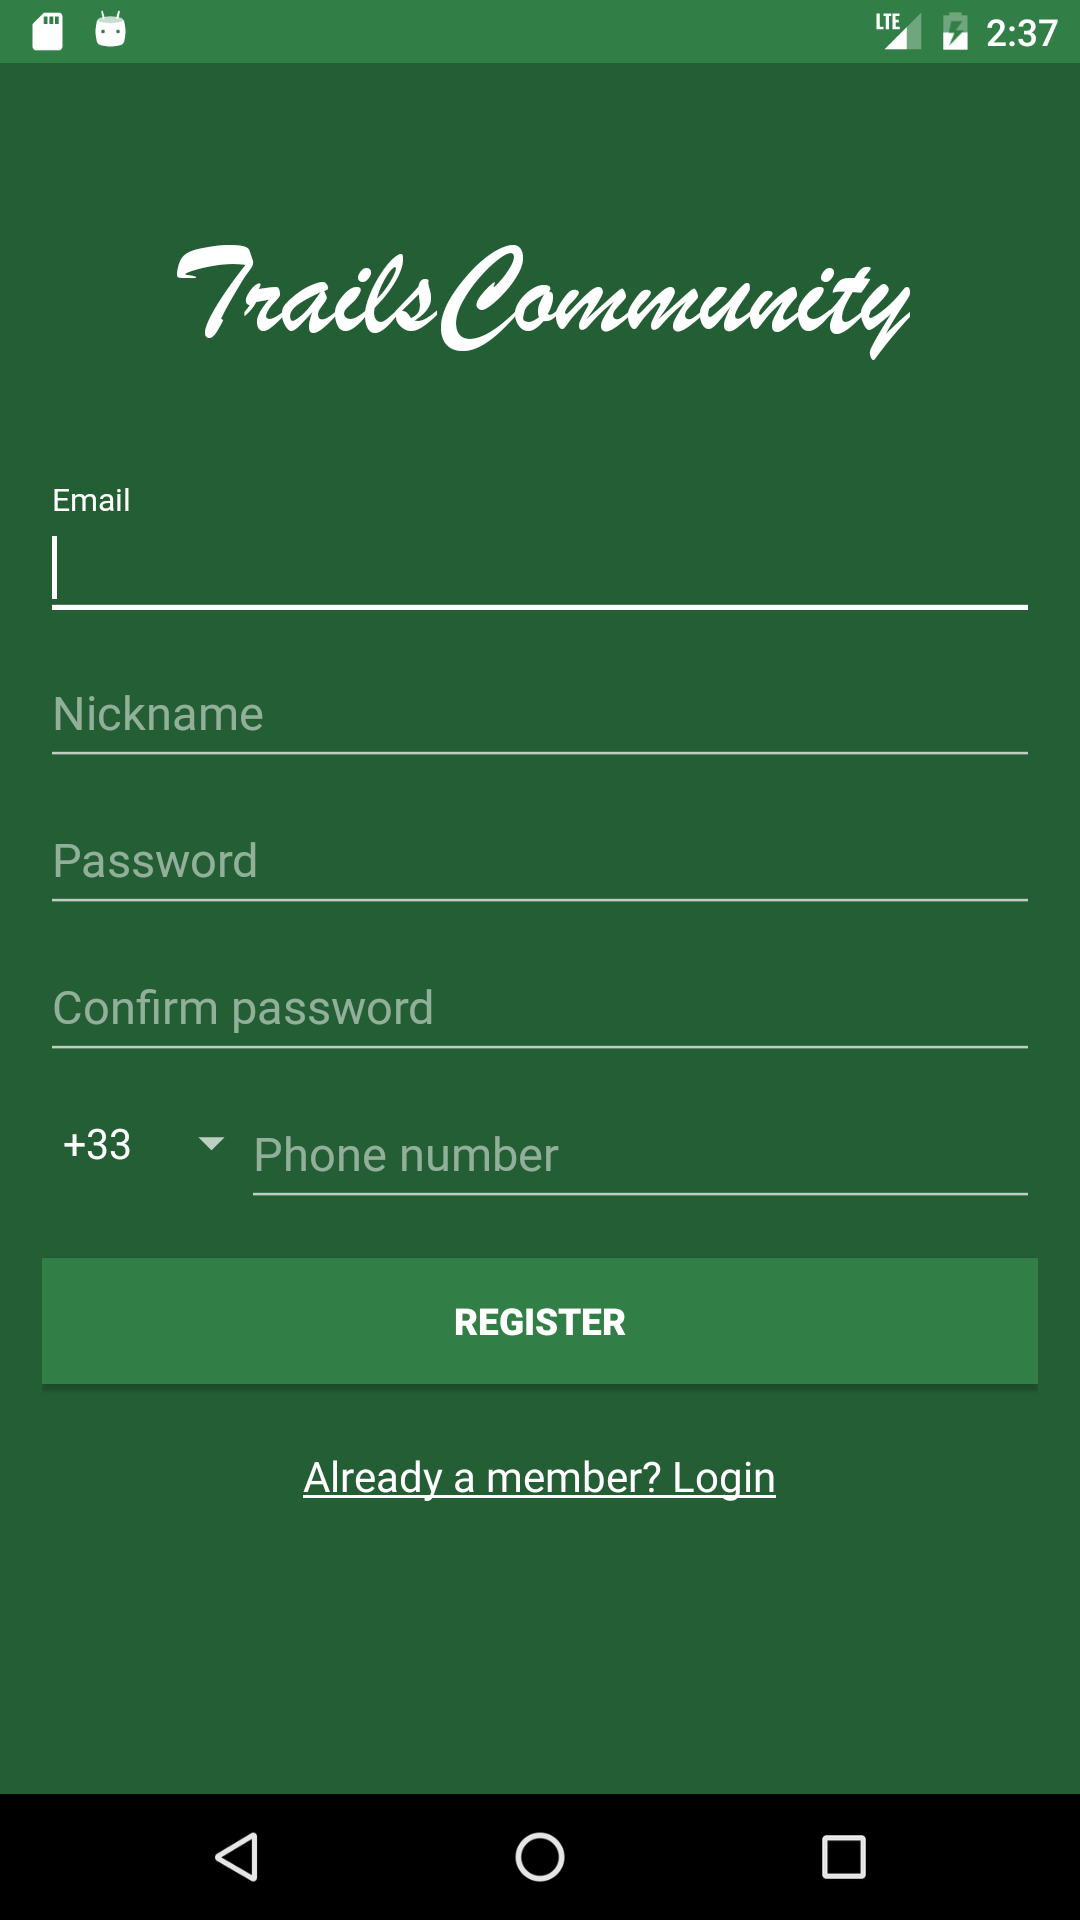
\includegraphics[scale=0.2]{Images/screenshots/register.png}
\end{figure}

\clearpage

\paragraph{}Une fois connecté, plusieurs choix s'offre à lui. Il peut alors sélectionner une session active pour la rejoindre ou visualiser son historique. Le bouton plus sur la barre de menu lui permet de créer une nouvelle session. D'autres fonctionnalités sont possible en cliquant sur le petit menu en haut à gauche.

%Capture d'écran de la page de l'ensemble des sessions%
\begin{figure}[!h]
	\caption{Diagramme de séquence de l'affichage de l'ensemble des sessions}
	\label{screenshots_list_session}
	\centering
	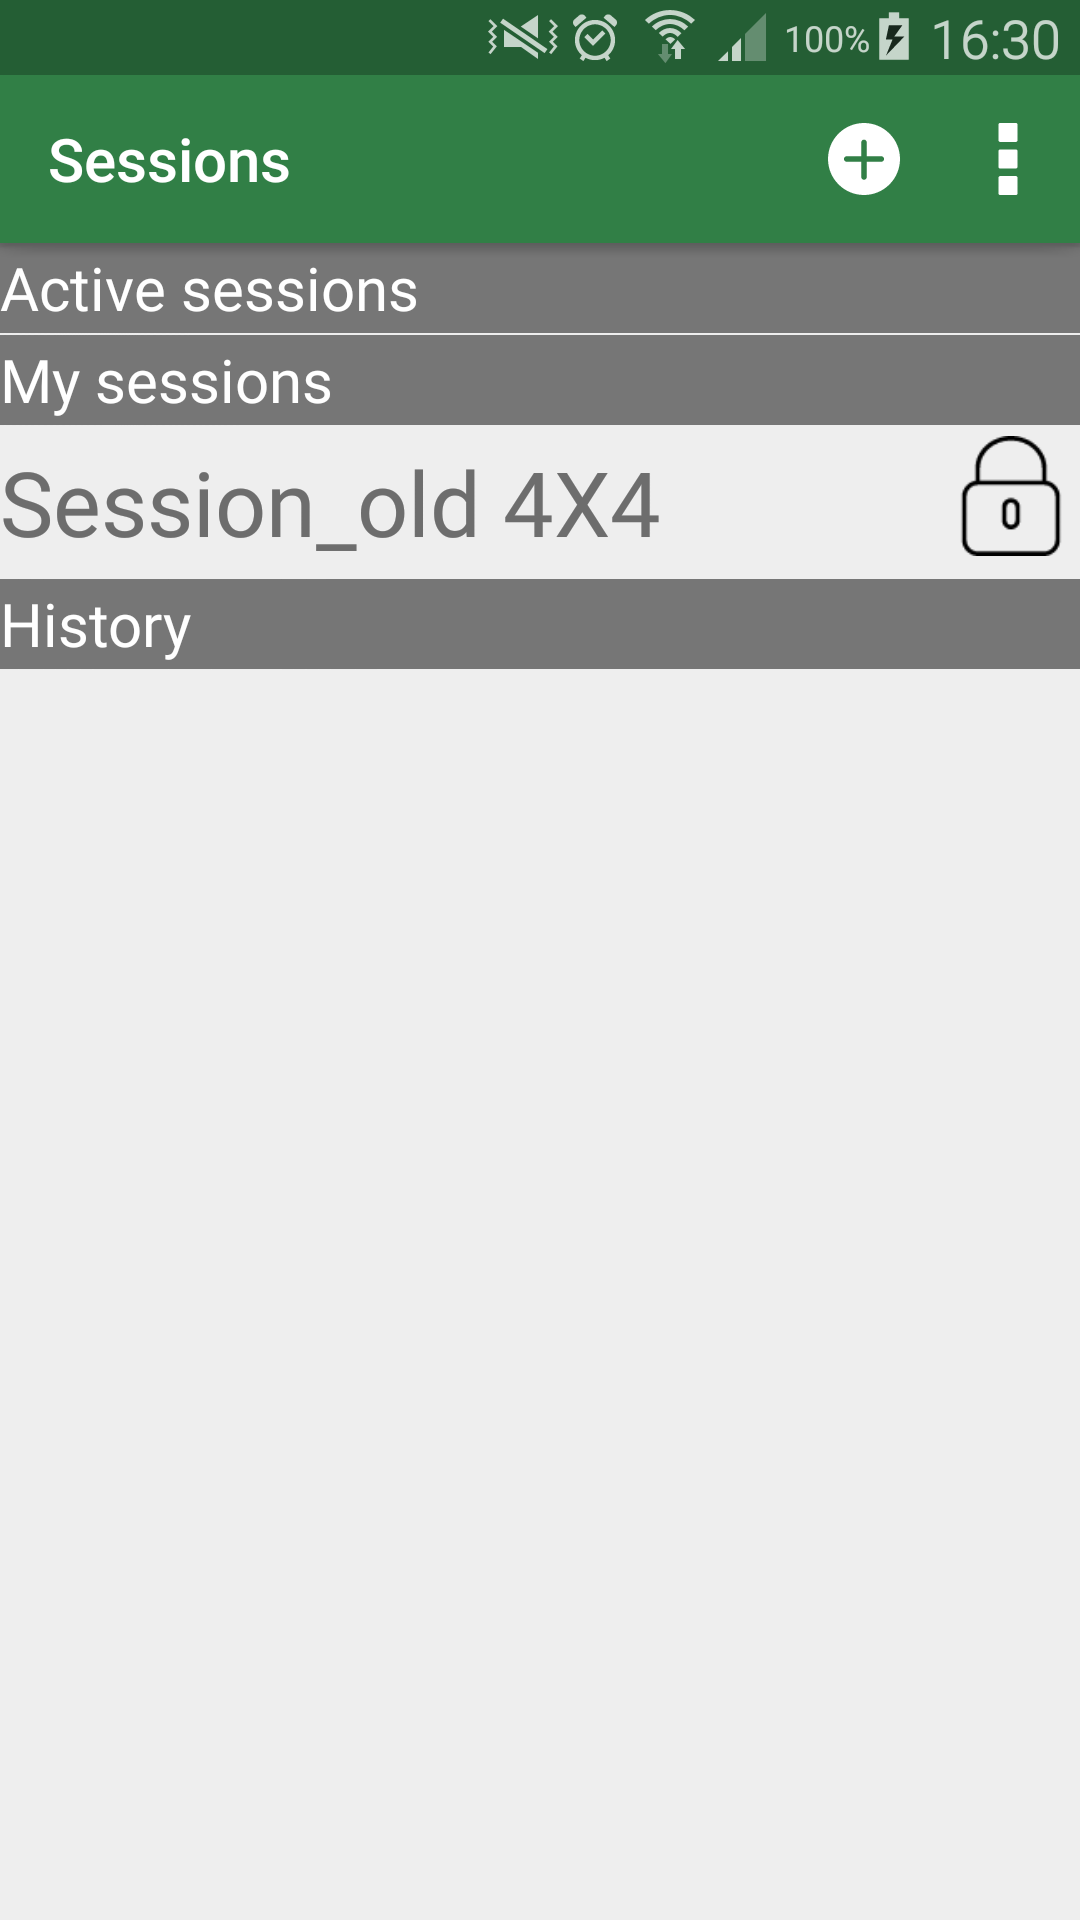
\includegraphics[scale=0.2]{Images/screenshots/list_sessions.png}
\end{figure}

\clearpage

\paragraph{}Pour la création d'une session, différentes informations cruciales sont demandées à l'utilisateur pour le bon déroulement de la futur session.
De plus, la modification des données de l'utilisateur courante ainsi que la déconnexion sont disponible depuis la sélection des sessions.

%Capture d'écran de la création d'une session%
\begin{figure}[!h]
	\caption{Capture d'écran de l'affichage de la création d'une session}
	\label{screenshots_create_session}
	\centering
	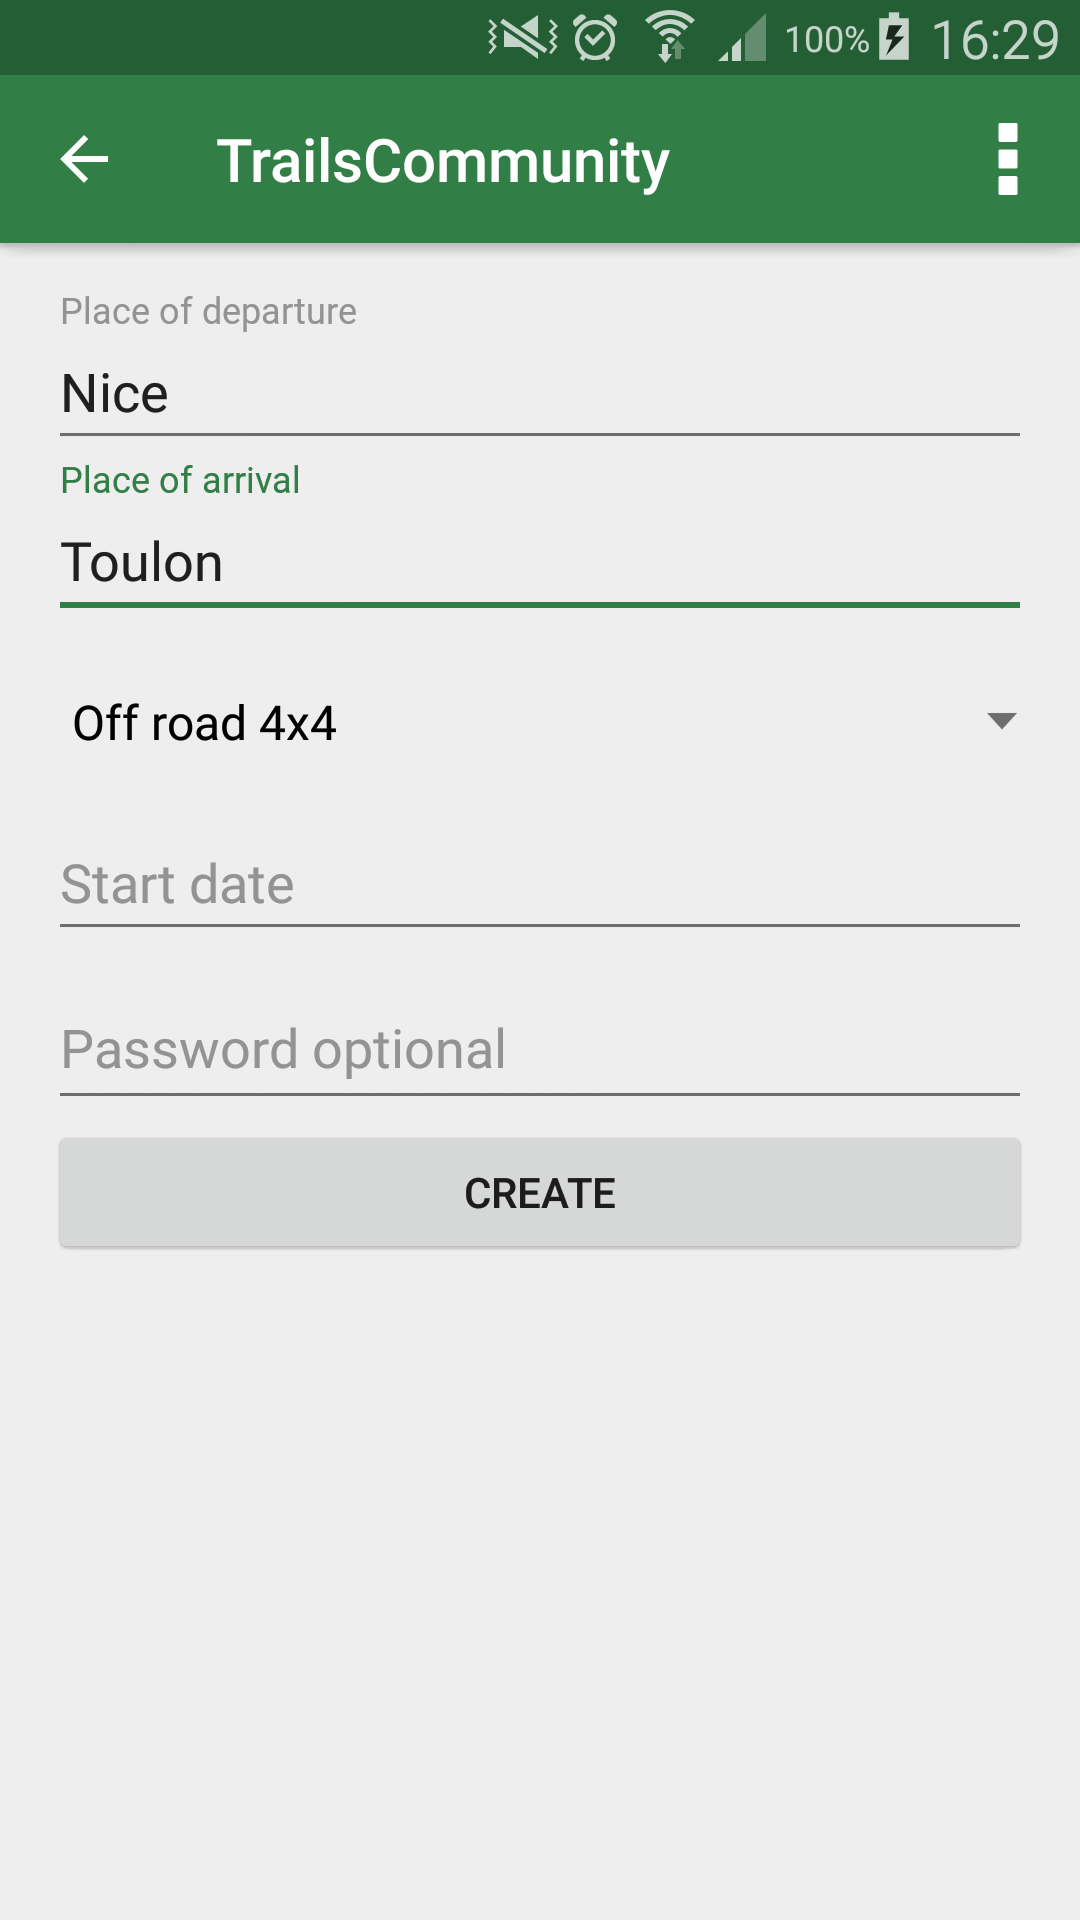
\includegraphics[scale=0.2]{Images/screenshots/create_session.png}
\end{figure}

\clearpage



%Capture d'écran de la deconnexion%
\begin{figure}[!h]
	\caption{Capture d'écran de l'affichage de la déconnexion}
	\label{screenshots_logout}
	\centering
	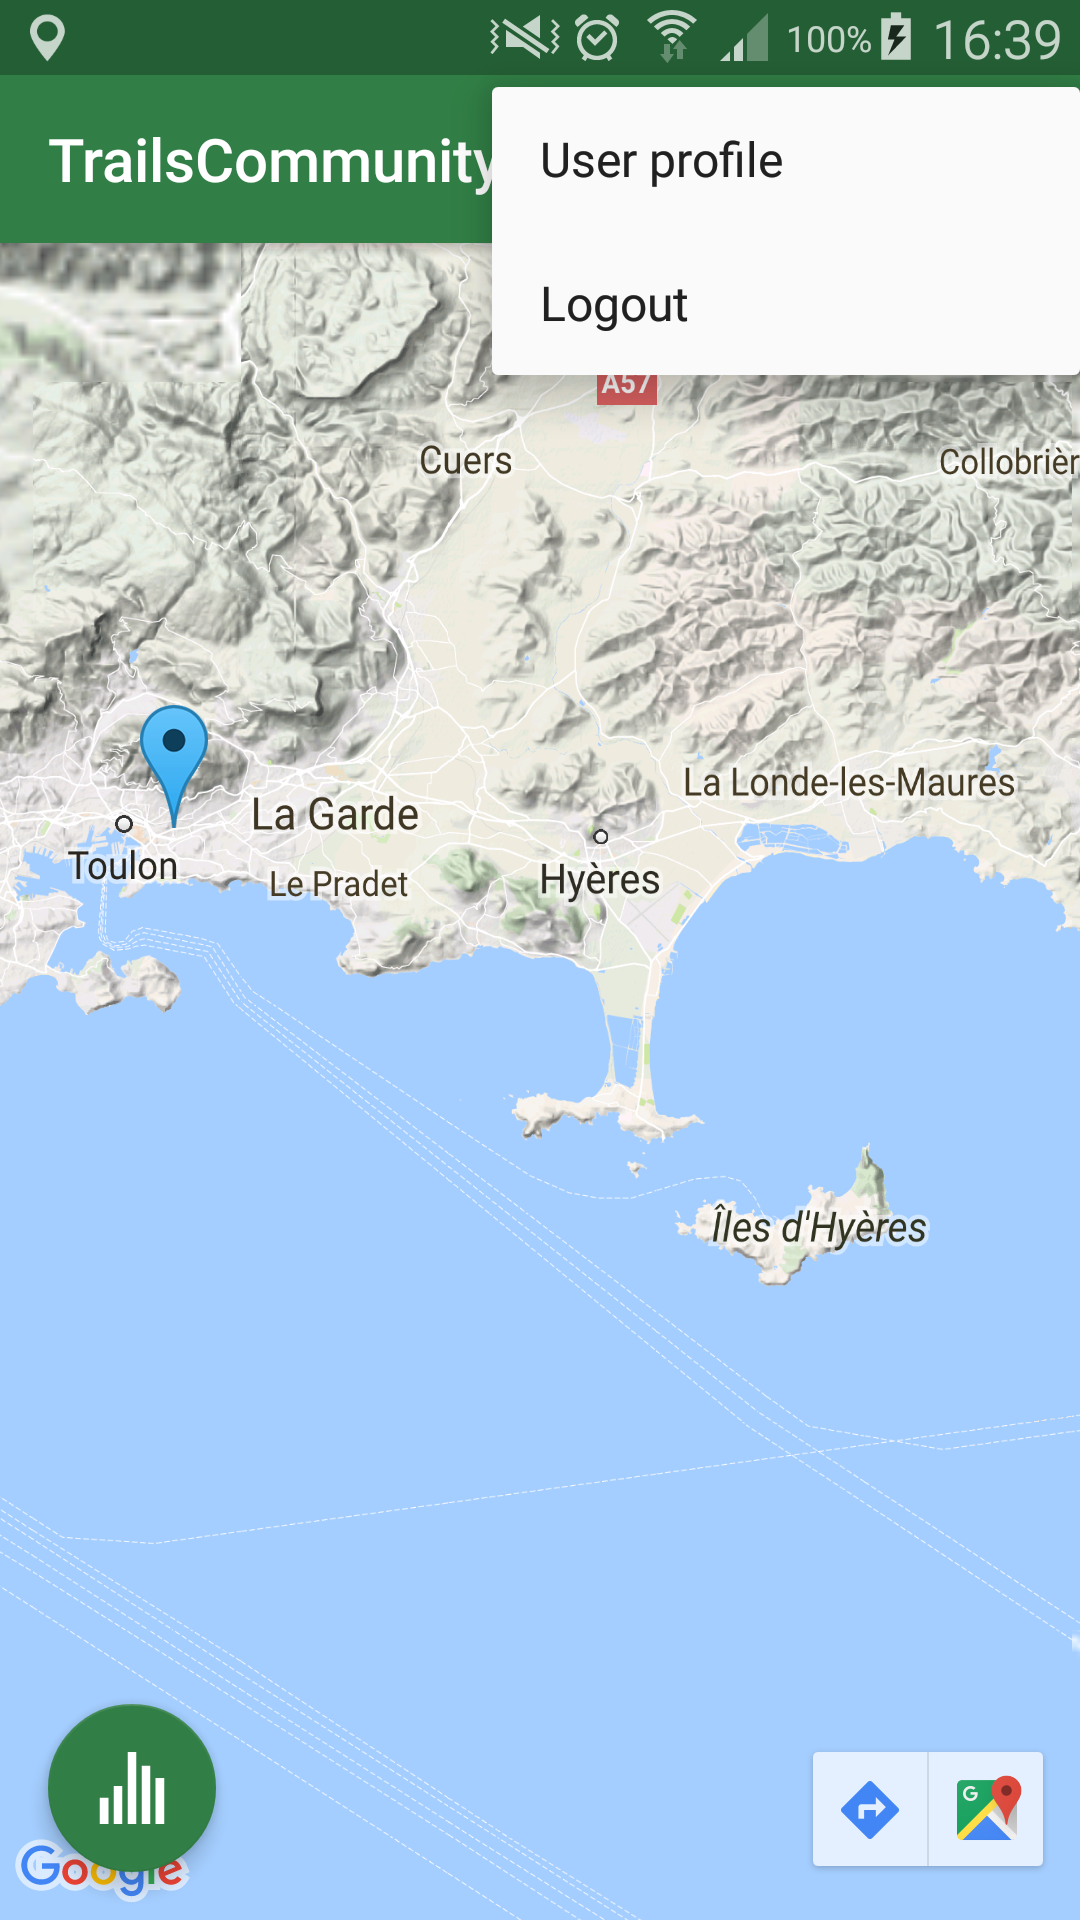
\includegraphics[scale=0.2]{Images/screenshots/logout.png}
\end{figure}

\clearpage

\paragraph{}Lors de la sélection d'une session, si la session est privé, l'application va alors demandée à l'utilisateur d'entrer le mot de passe de la session.

%Capture d'écran de la popup password%
\begin{figure}[!h]
	\caption{Capture d'écran de l'affichage de la popup de l'entrée du mot de passe}
	\label{screenshots_password}
	\centering
	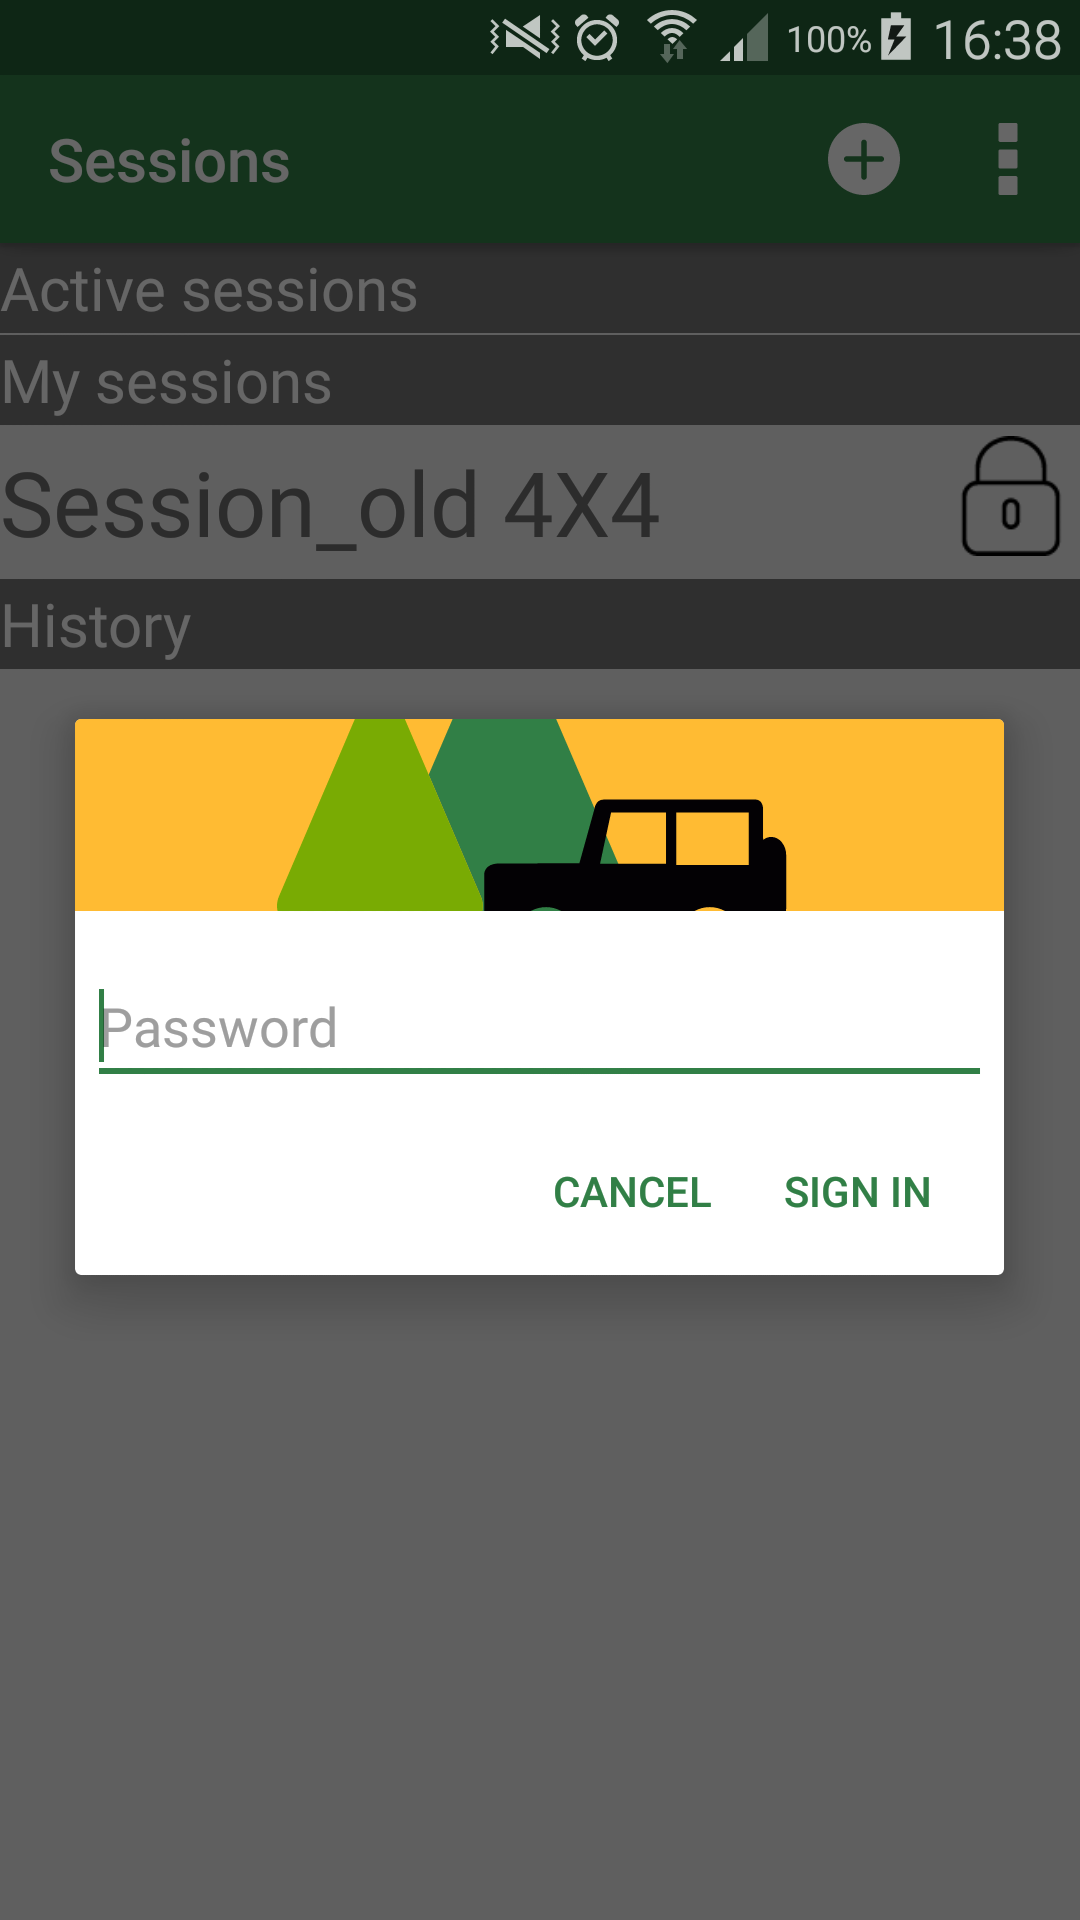
\includegraphics[scale=0.2]{Images/screenshots/password.png}
\end{figure}

\clearpage

\paragraph{}Une fois le mot de passe correct, une Google maps s'affiche avec l'ensemble des tracés des différents participants. Différents boutons sont disponible dans la barre de menu pour afficher le chat ou pour modifier les données de l'utilisateur courant. De plus, les statistiques sont disponibles lorsque l'utilisateur clique sur le bouton flottant en bas à gauche.

%Captue d'écran de la google map%
\begin{figure}[!h]
	\caption{Capture d'écran de l'affichage d'une session}
	\label{screenshots_session}
	\centering
	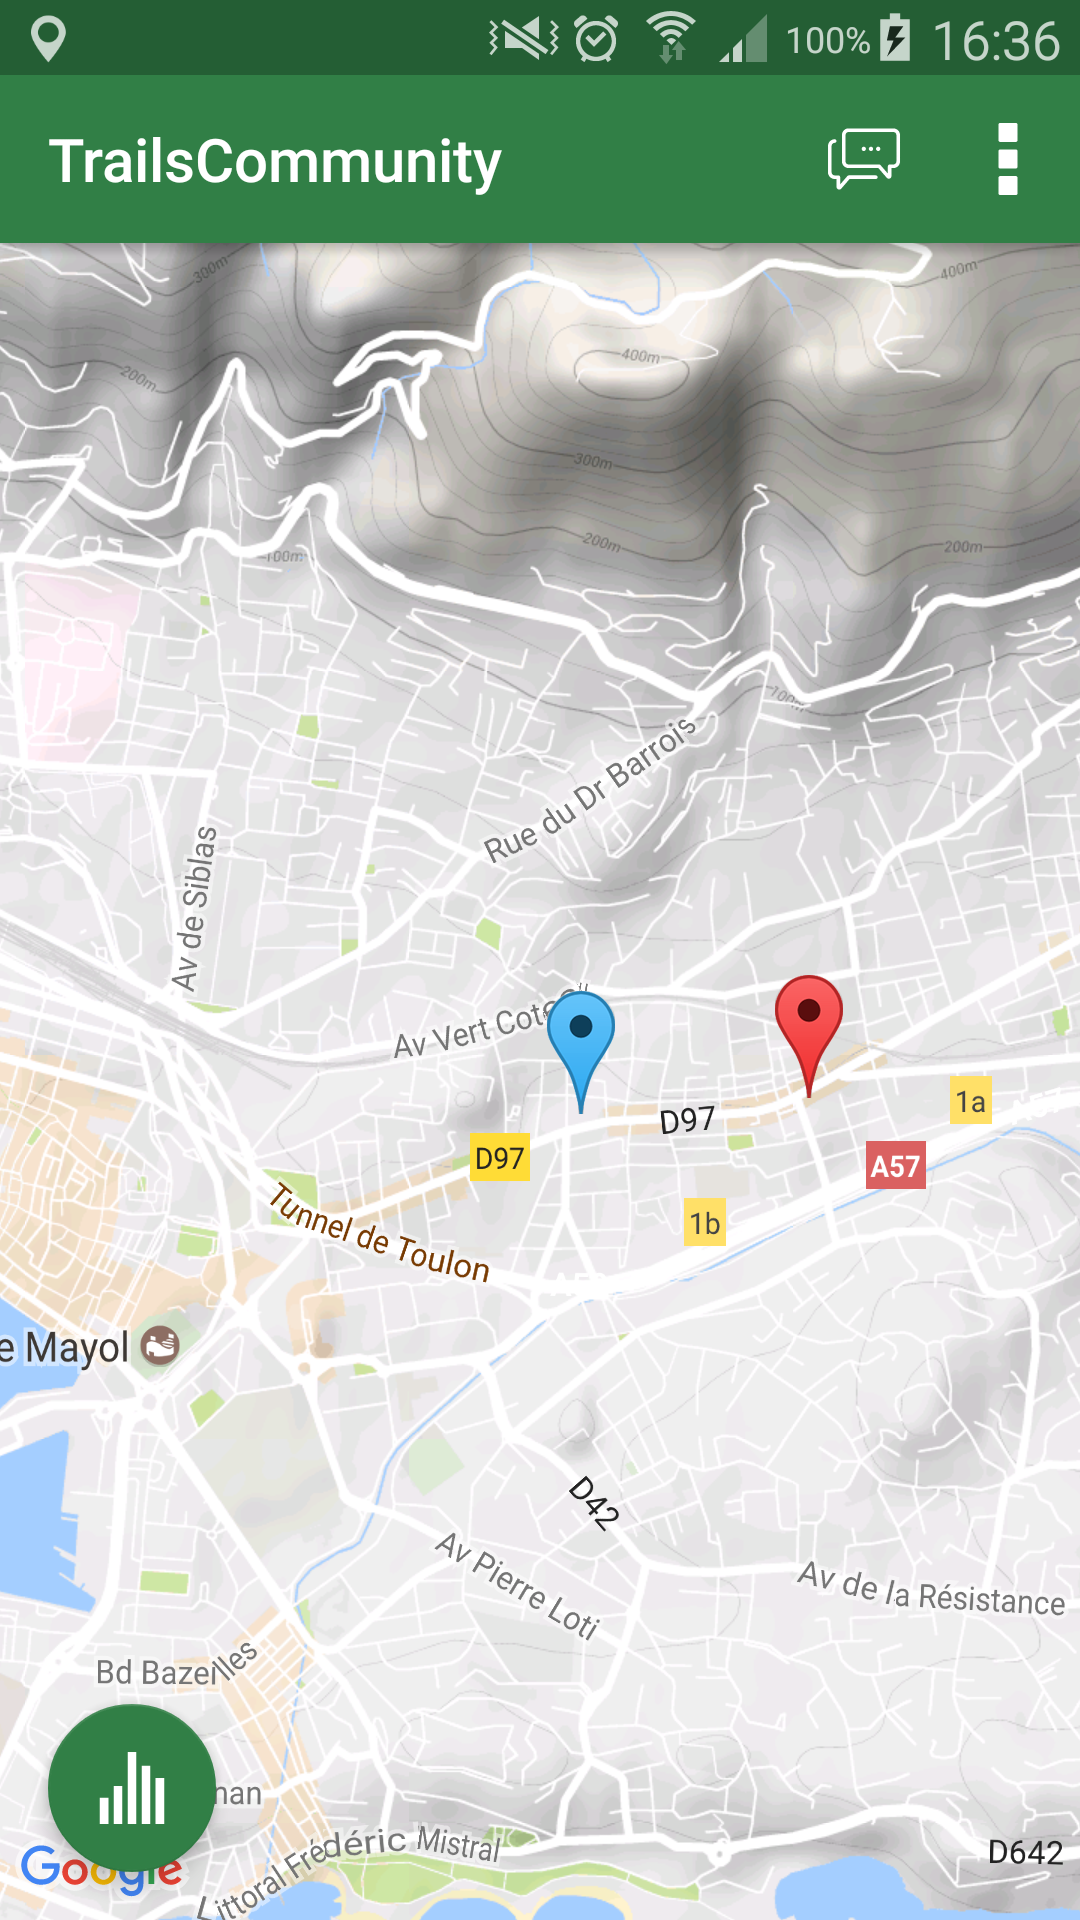
\includegraphics[scale=0.2]{Images/screenshots/session.png}
\end{figure}

\clearpage


%Capture d'écran du chat%
\begin{figure}[!h]
	\caption{Capture d'écran de l'affichage du chat}
	\label{screenshots_chat}
	\centering
	\includegraphics[scale=0.2]{Images/screenshots/chat.png}
\end{figure}

\clearpage


%Capture d'écran des statistiques%
\begin{figure}[!h]
	\caption{Capture d'écran de l'affichage des statistiques}
	\label{screenshots_statistics}
	\centering
	\includegraphics[scale=0.2]{Images/screenshots/statistics.png}
\end{figure}

\clearpage


\part{Déroulement du projet}

\section{Difficultés rencontrées}

\paragraph{}La principale difficulté que nous avons eu lors de la réalisation de ce projet a été de maintenir une cohérence entre les diagrammes UML réalisés lors de la première partie du projet et le code Java réalisé par la suite. Cependant, l'expérience engrangé lors de la réalisation de notre premier projet UML nous à permit d'obtenir un certain recul pour éviter les différents problèmes rencontrés précédemment.
Il a donc été nécessaire de reprendre et de mettre à jour la plupart des diagrammes UML après avoir commencé à mettre en place l'application Android.

\paragraph{}La seconde partie de difficulté est liée à l'utilisation de nouvelles technologies :
\begin{itemize}
	\item Mise en place d'un serveur afin d'obtenir un service utilisant une architecture propre à notre application mobile : utilisation de Ruby.
	\item Utilisation du système d'annotation d'Android permettant une meilleurs lisibilité du code d'une part et donc une meilleur maintenance et d'autre part une meilleur injection.
	\item de nombreuse dépendances et librairies on été ajoutés dans le projet Android. 
\end{itemize}

Globalement, l'avancée du projet a été assez fluide malgré ces difficultés. La mise en commun de nos connaissances et de nos expériences précédentes nous a permis d'atteindre la majorités des objectifs que nous nous étions fixés.

\section{Perspectives d'évolution}

L'application mobile possède les fonctionnalités qui permettent de rejoindre une session et d'y participer d'une manière tout a fait normal, cependant de nombreuses améliorations peuvent lui être apportés comme :
\begin{itemize}
	\item La modification des données des sessions et des utilisateurs.
	\item La création d'un site web permettant aux organisateurs de gérer et de collecter l'ensemble des informations des sessions en cours de réalisation.
\end{itemize}

\section{Conclusion}

\paragraph{}La conduite de ce projet nous aura permis de confirmé nos compétences UML utilisé lors du projet précédent. De nombreux problèmes ont pu donc être résolu plus rapidement ou tout simplement évité.
De plus, l'ensemble de nos compétences en Java on pu être appliqué sur un projet Android concret englobant l'ensemble des compétences vu lors du module prévu à cet effet.
La réalisation de ce projet, en plus de nous avoir aidé à utiliser de nouveaux outils et de nouvelles connaissances, nous a également permis de conduire un projet plus ambitieux que prévu depuis la phase de conception jusqu'à l'implémentation, dans un délai relativement court. 


\part{Annexe - Diagrammes UML}

\chapter{Diagrammes généraux}

\begin{figure}[!h]
	\caption{Diagramme d'architecture de l'API}
	\label{API_architecture}
	\centering
	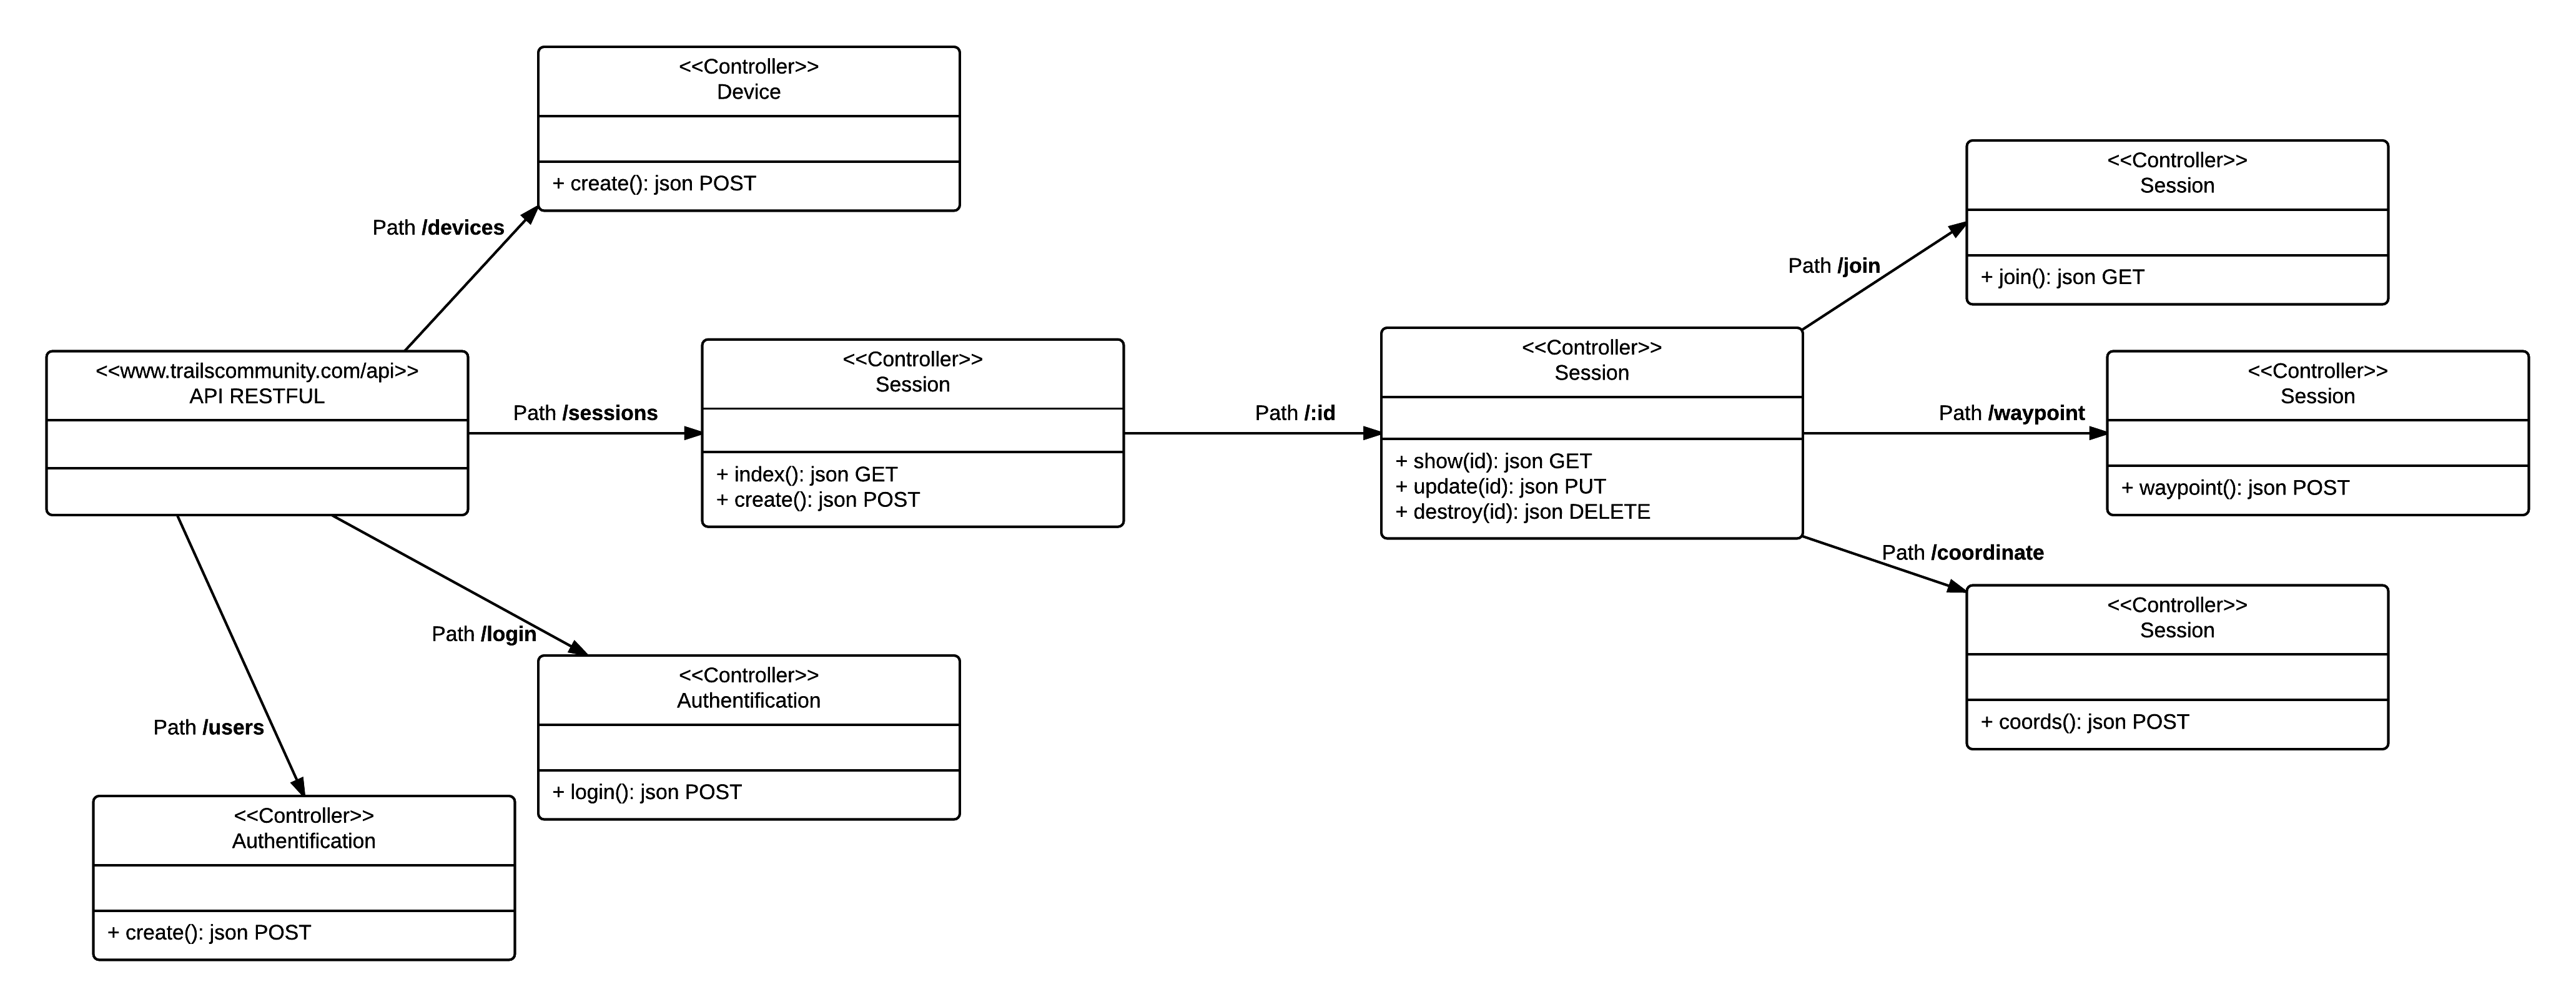
\includegraphics[scale=0.5]{Images/diagram/API_architecture.png}
\end{figure}

\chapter{Modélisation serveur}

\begin{figure}[!h]
	\caption{Diagramme de séquence pour la vérification de la cohérence des données entre le client et le serveur}
	\label{check_consitency_data_client_serveur_sequence_diagram}
	\centering
	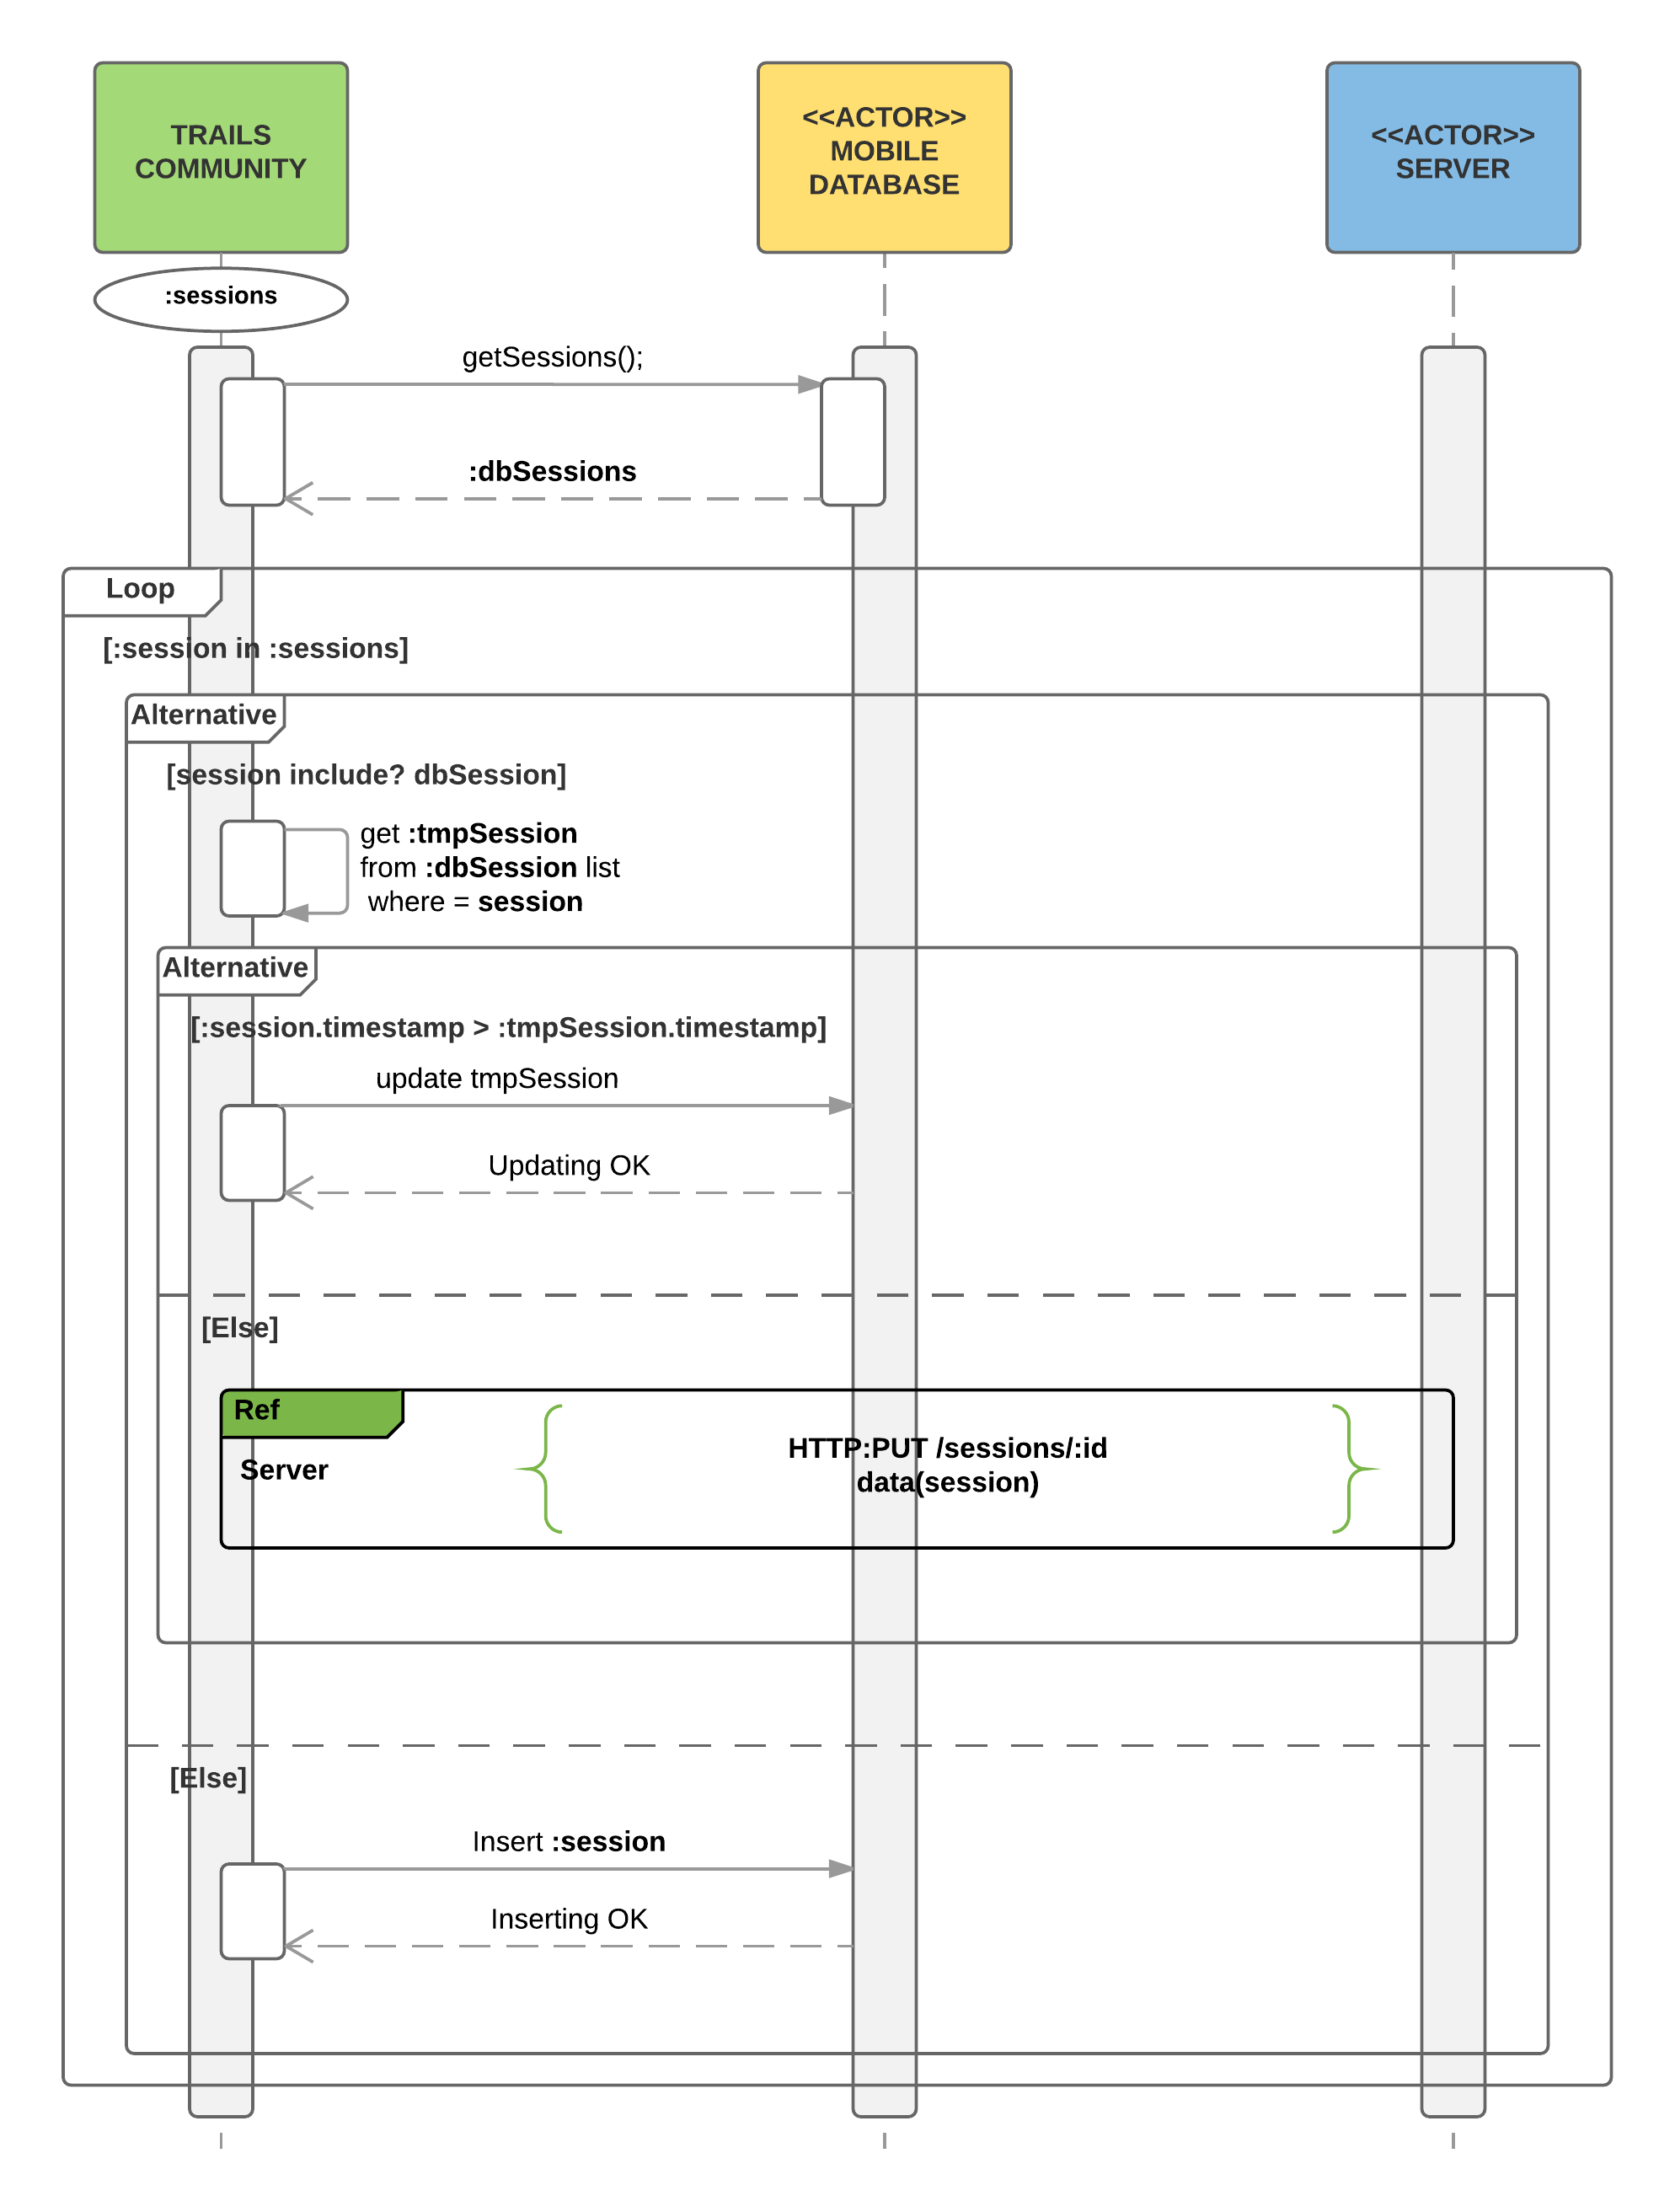
\includegraphics[scale=0.6]{Images/diagram/check_consistency_data_client_server_sequence_diagram.png}
\end{figure} 

\chapter{Diagrammes de séquences}

\begin{figure}[!h]
	\caption{Diagramme de séquence de l'ajout d'un waypoint}
	\label{add_waypoint_sequence_diagram}
	\centering
	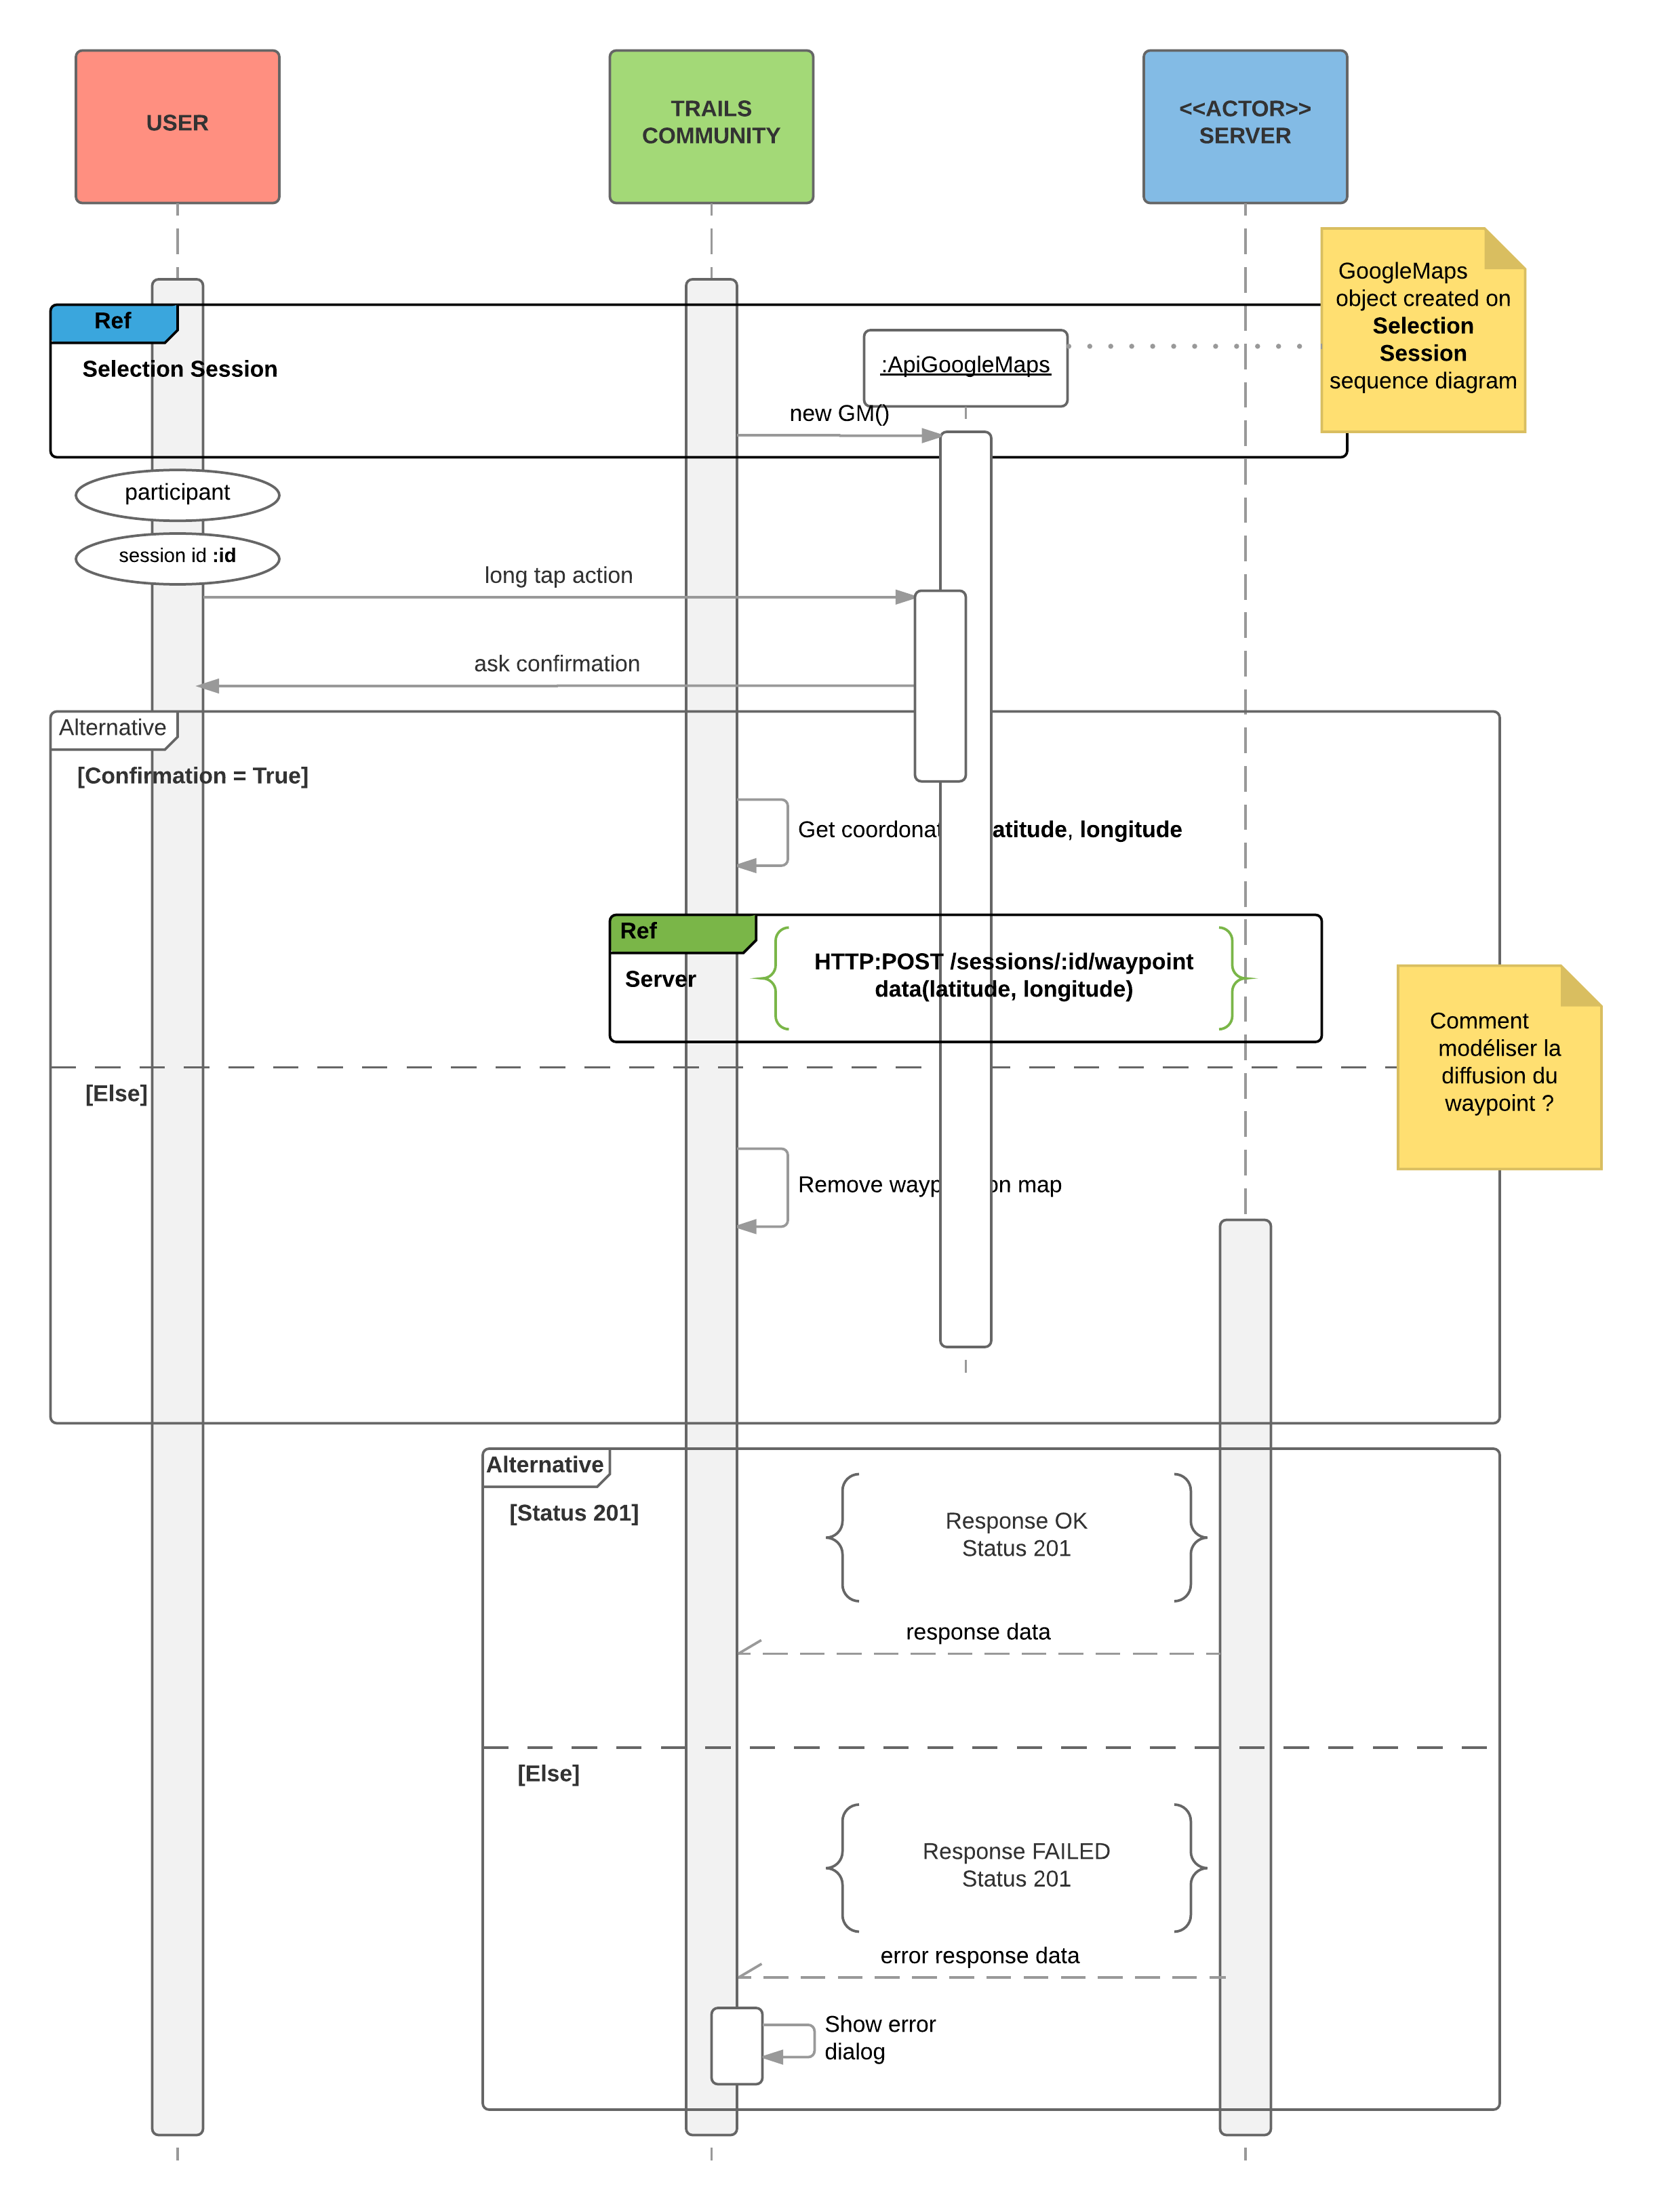
\includegraphics[scale=0.2]{Images/diagram/add_waypoint_sequence_diagram.png}
\end{figure}

\begin{figure}[!h]
	\caption{Diagramme de séquence du chat}
	\label{chat_sequence_diagram}
	\centering
	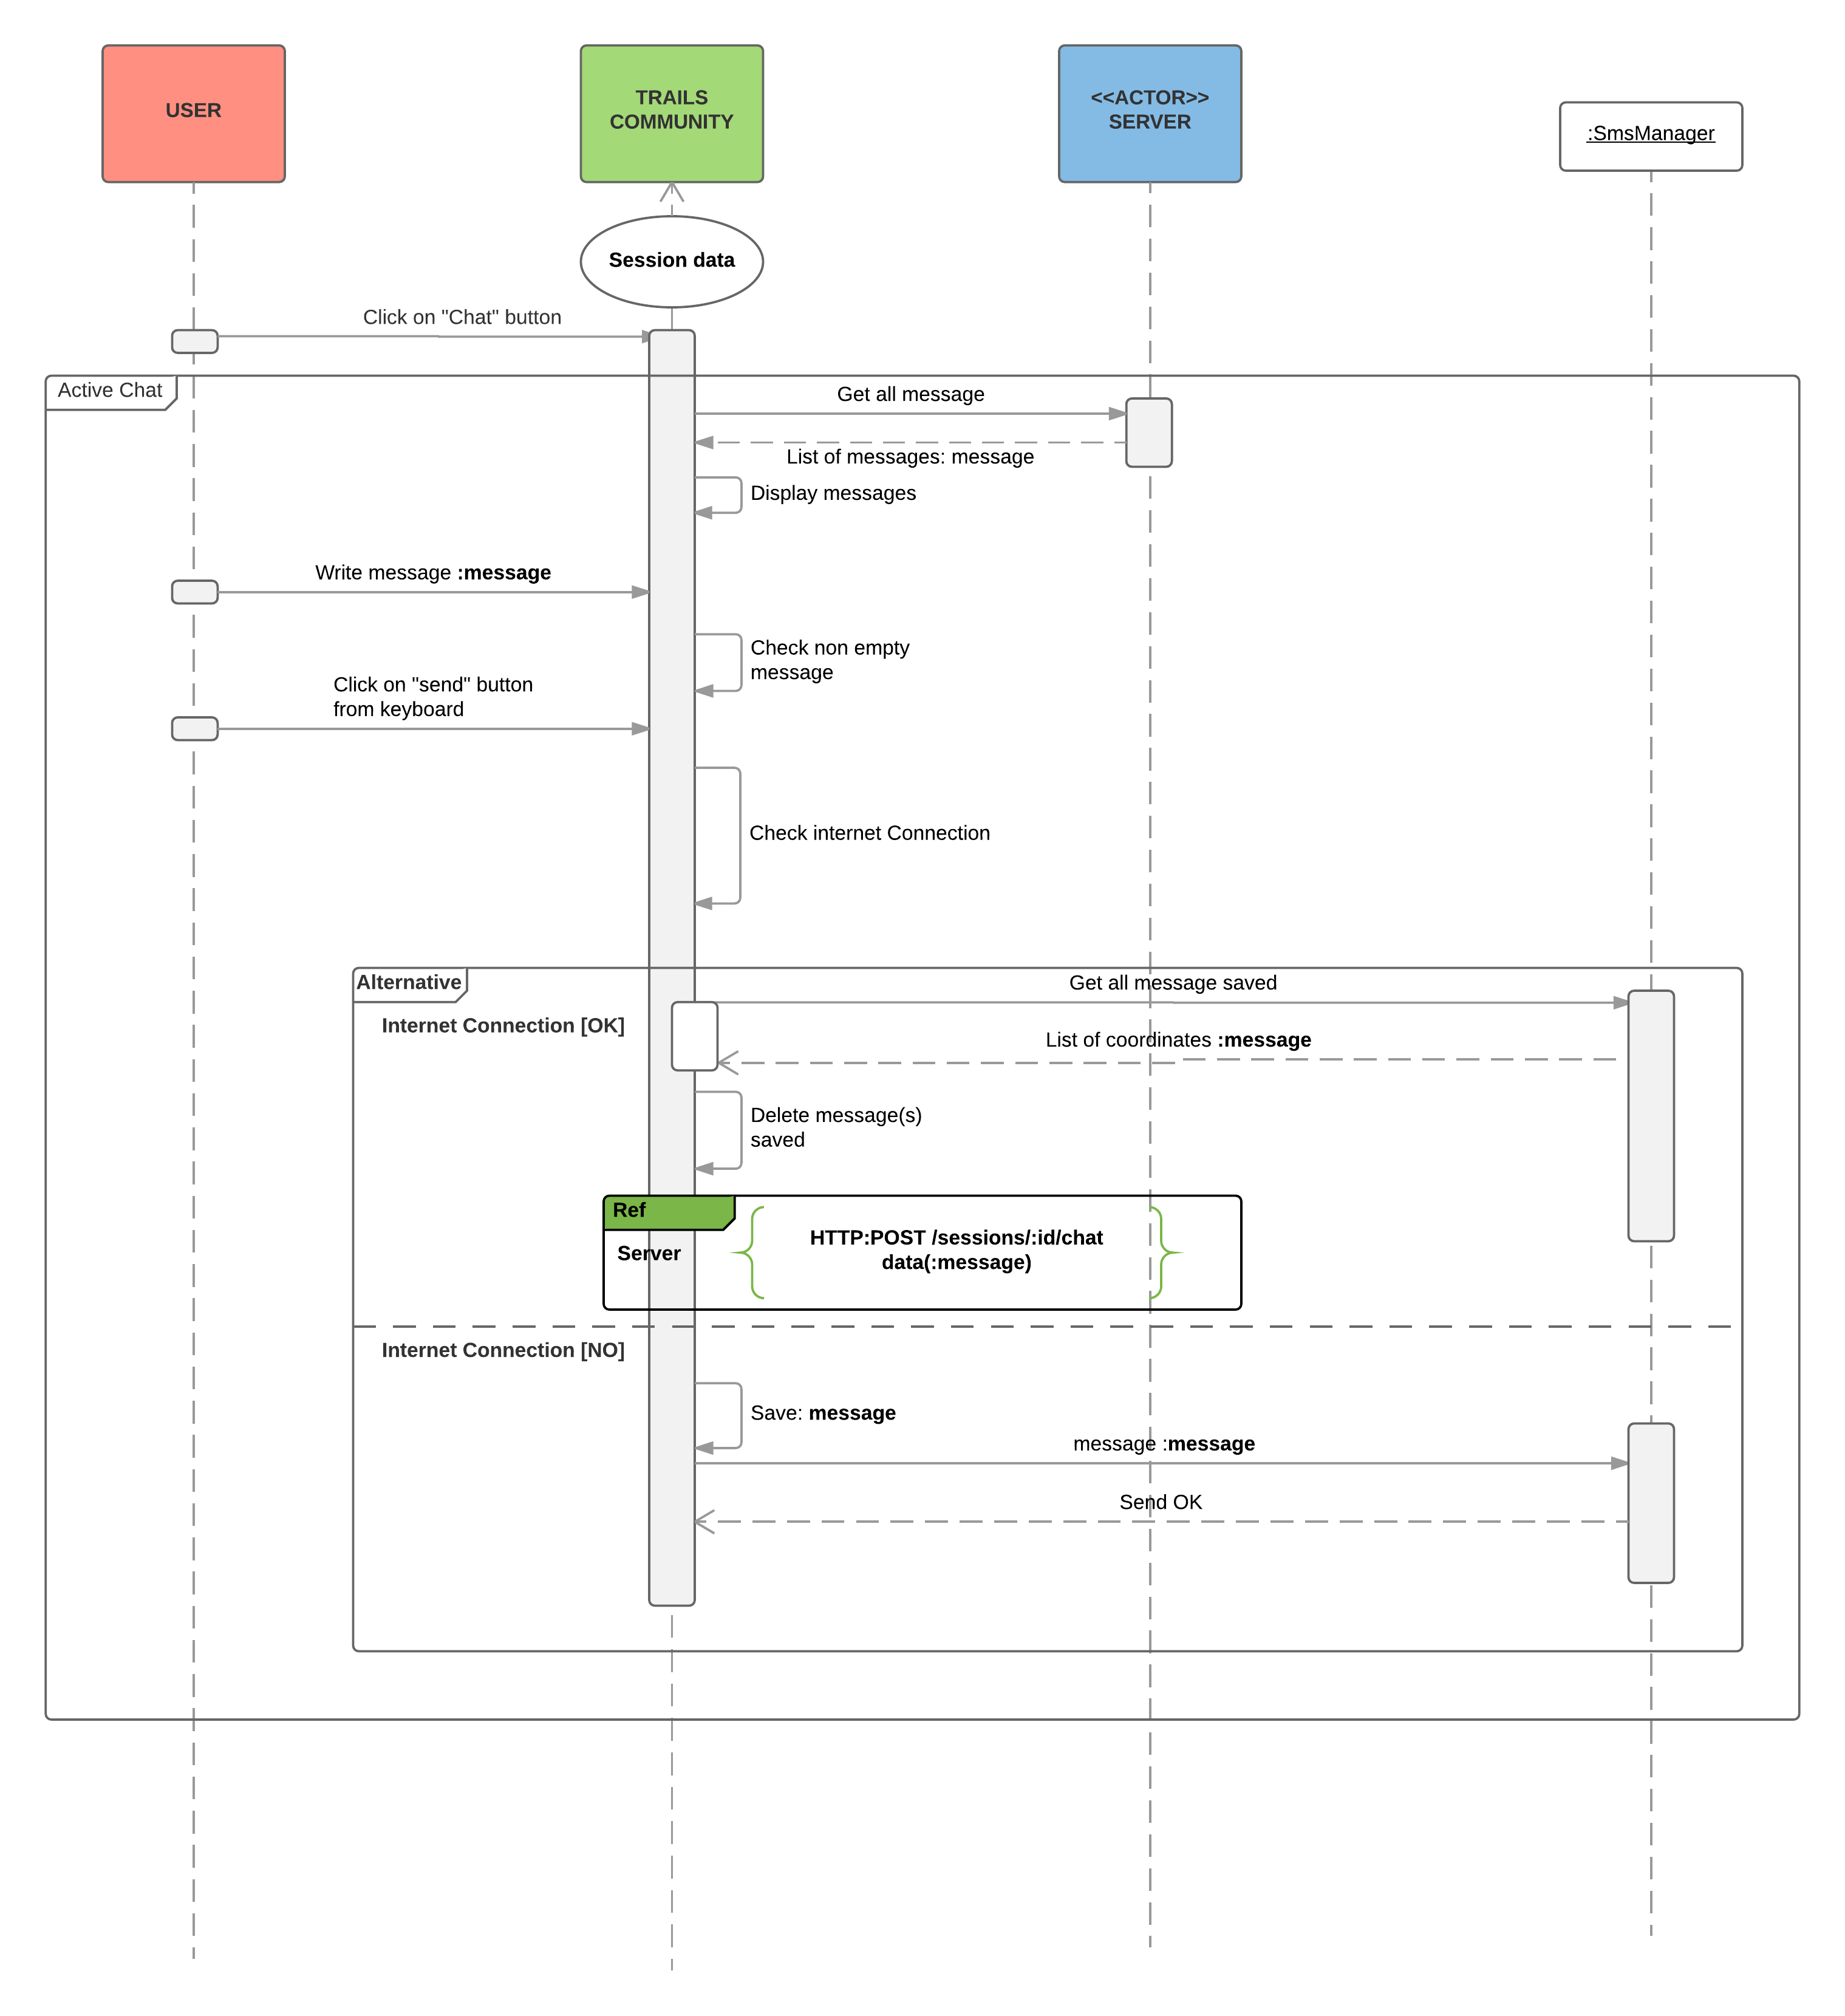
\includegraphics[scale=0.7]{Images/diagram/chat_sequence_diagram.png}
\end{figure}

\begin{figure}[!h]
	\caption{Diagramme de séquence du la modification du profile}
	\label{modify_profil_sequence_diagram}
	\centering
	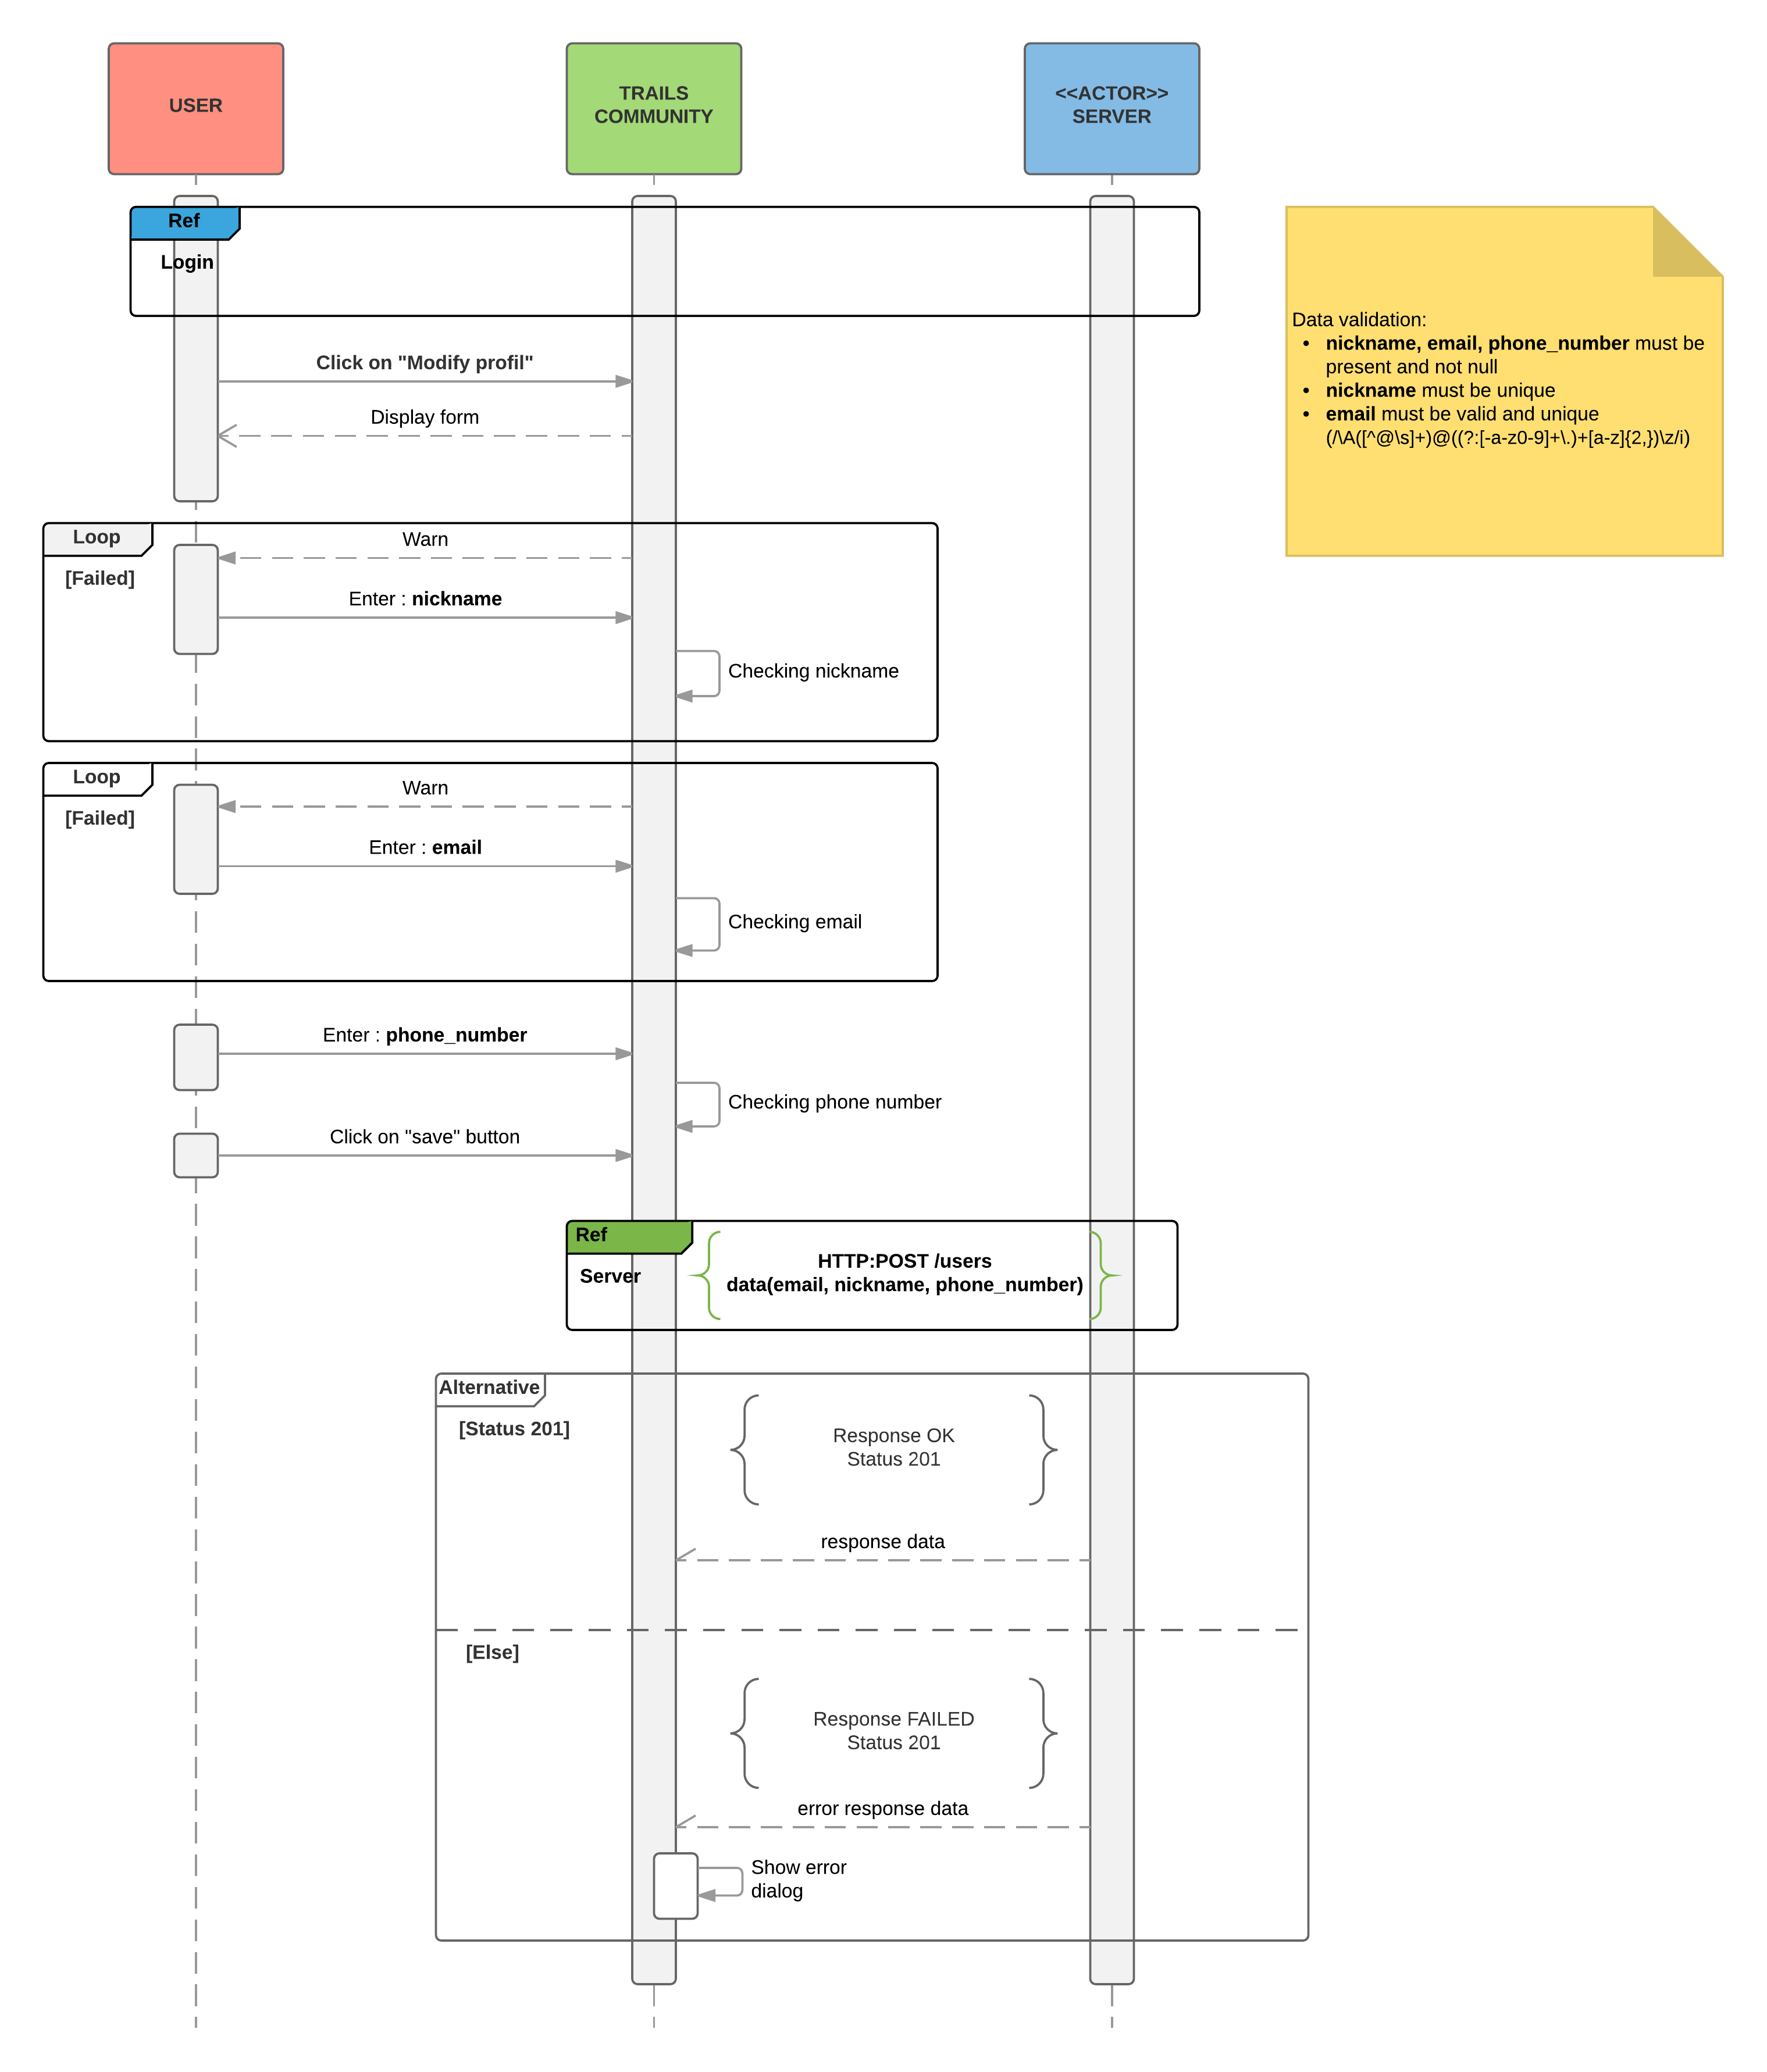
\includegraphics[scale=0.7]{Images/diagram/modify_profil_sequence_diagram.png}
\end{figure}

\begin{figure}[!h]
	\caption{Diagramme de séquence pour la sélection d'une session}
	\label{select_session_sequence_diagram}
	\centering
	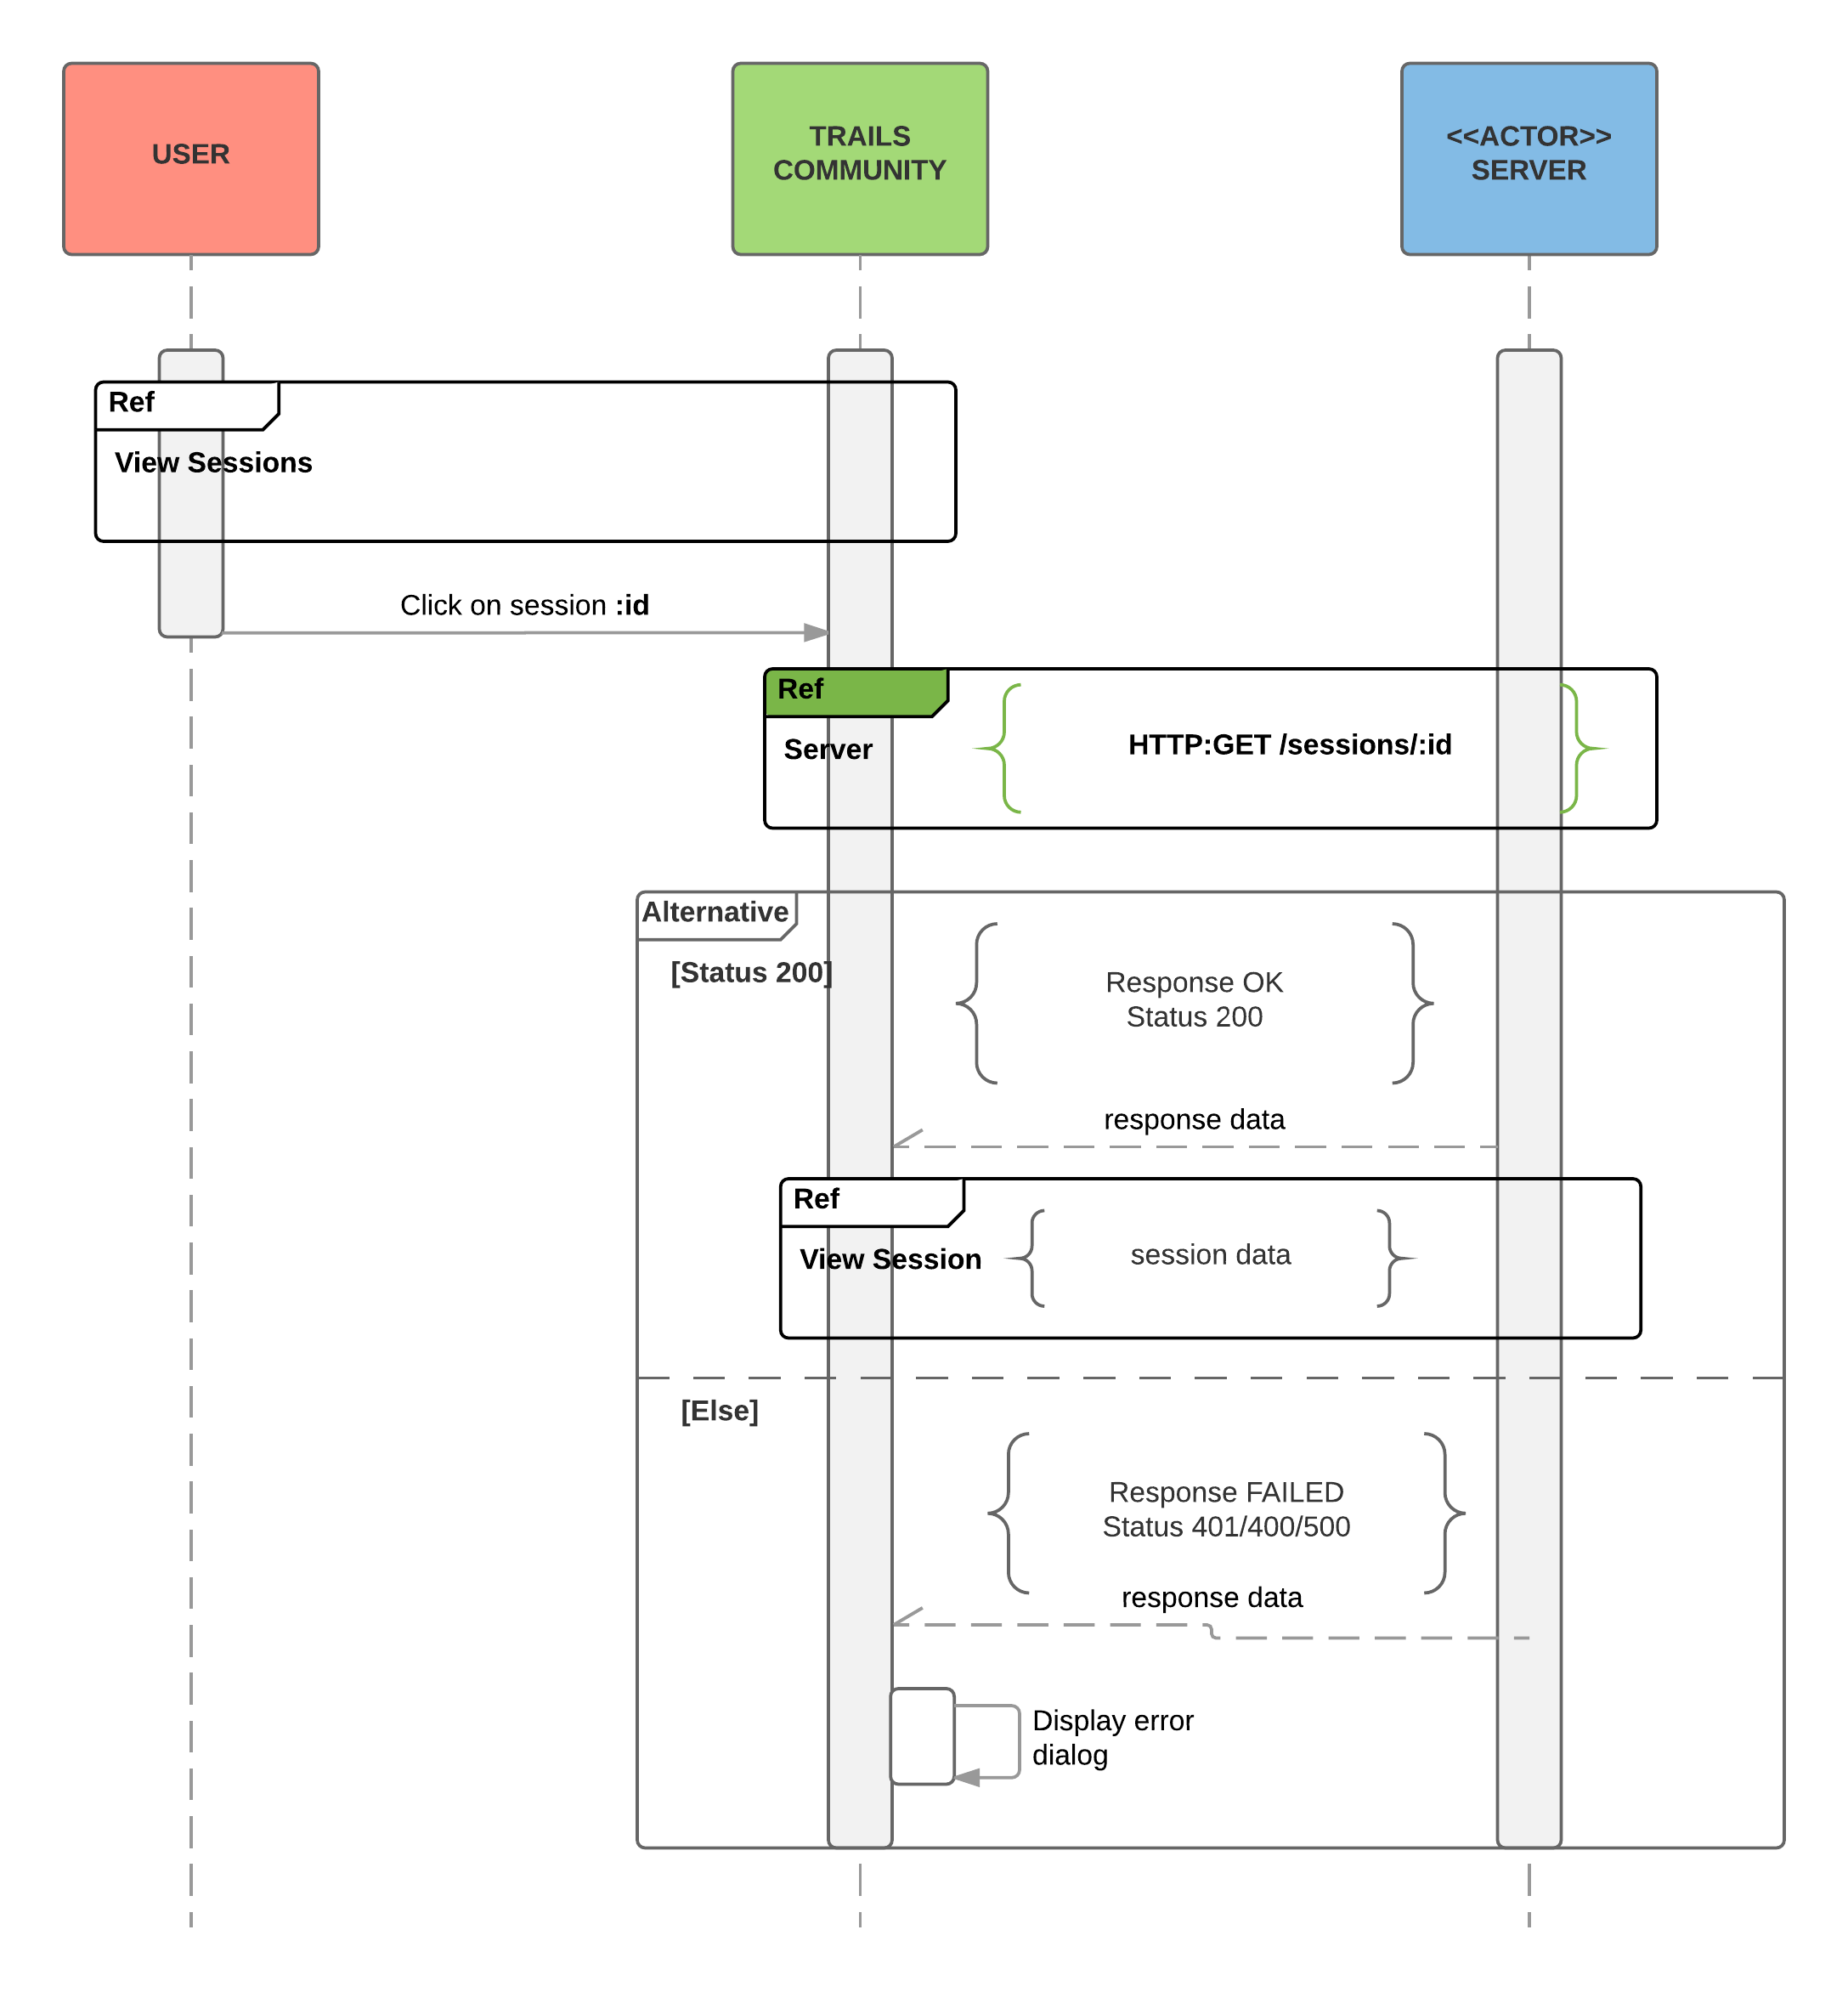
\includegraphics[scale=0.5]{Images/diagram/selection_session_sequence_diagram.png}
\end{figure}

\begin{figure}[!h]
	\caption{Diagramme de séquence pour l'utilisation de la géolocalisation}
	\label{user_geolocalisation_sequence_diagram}
	\centering
	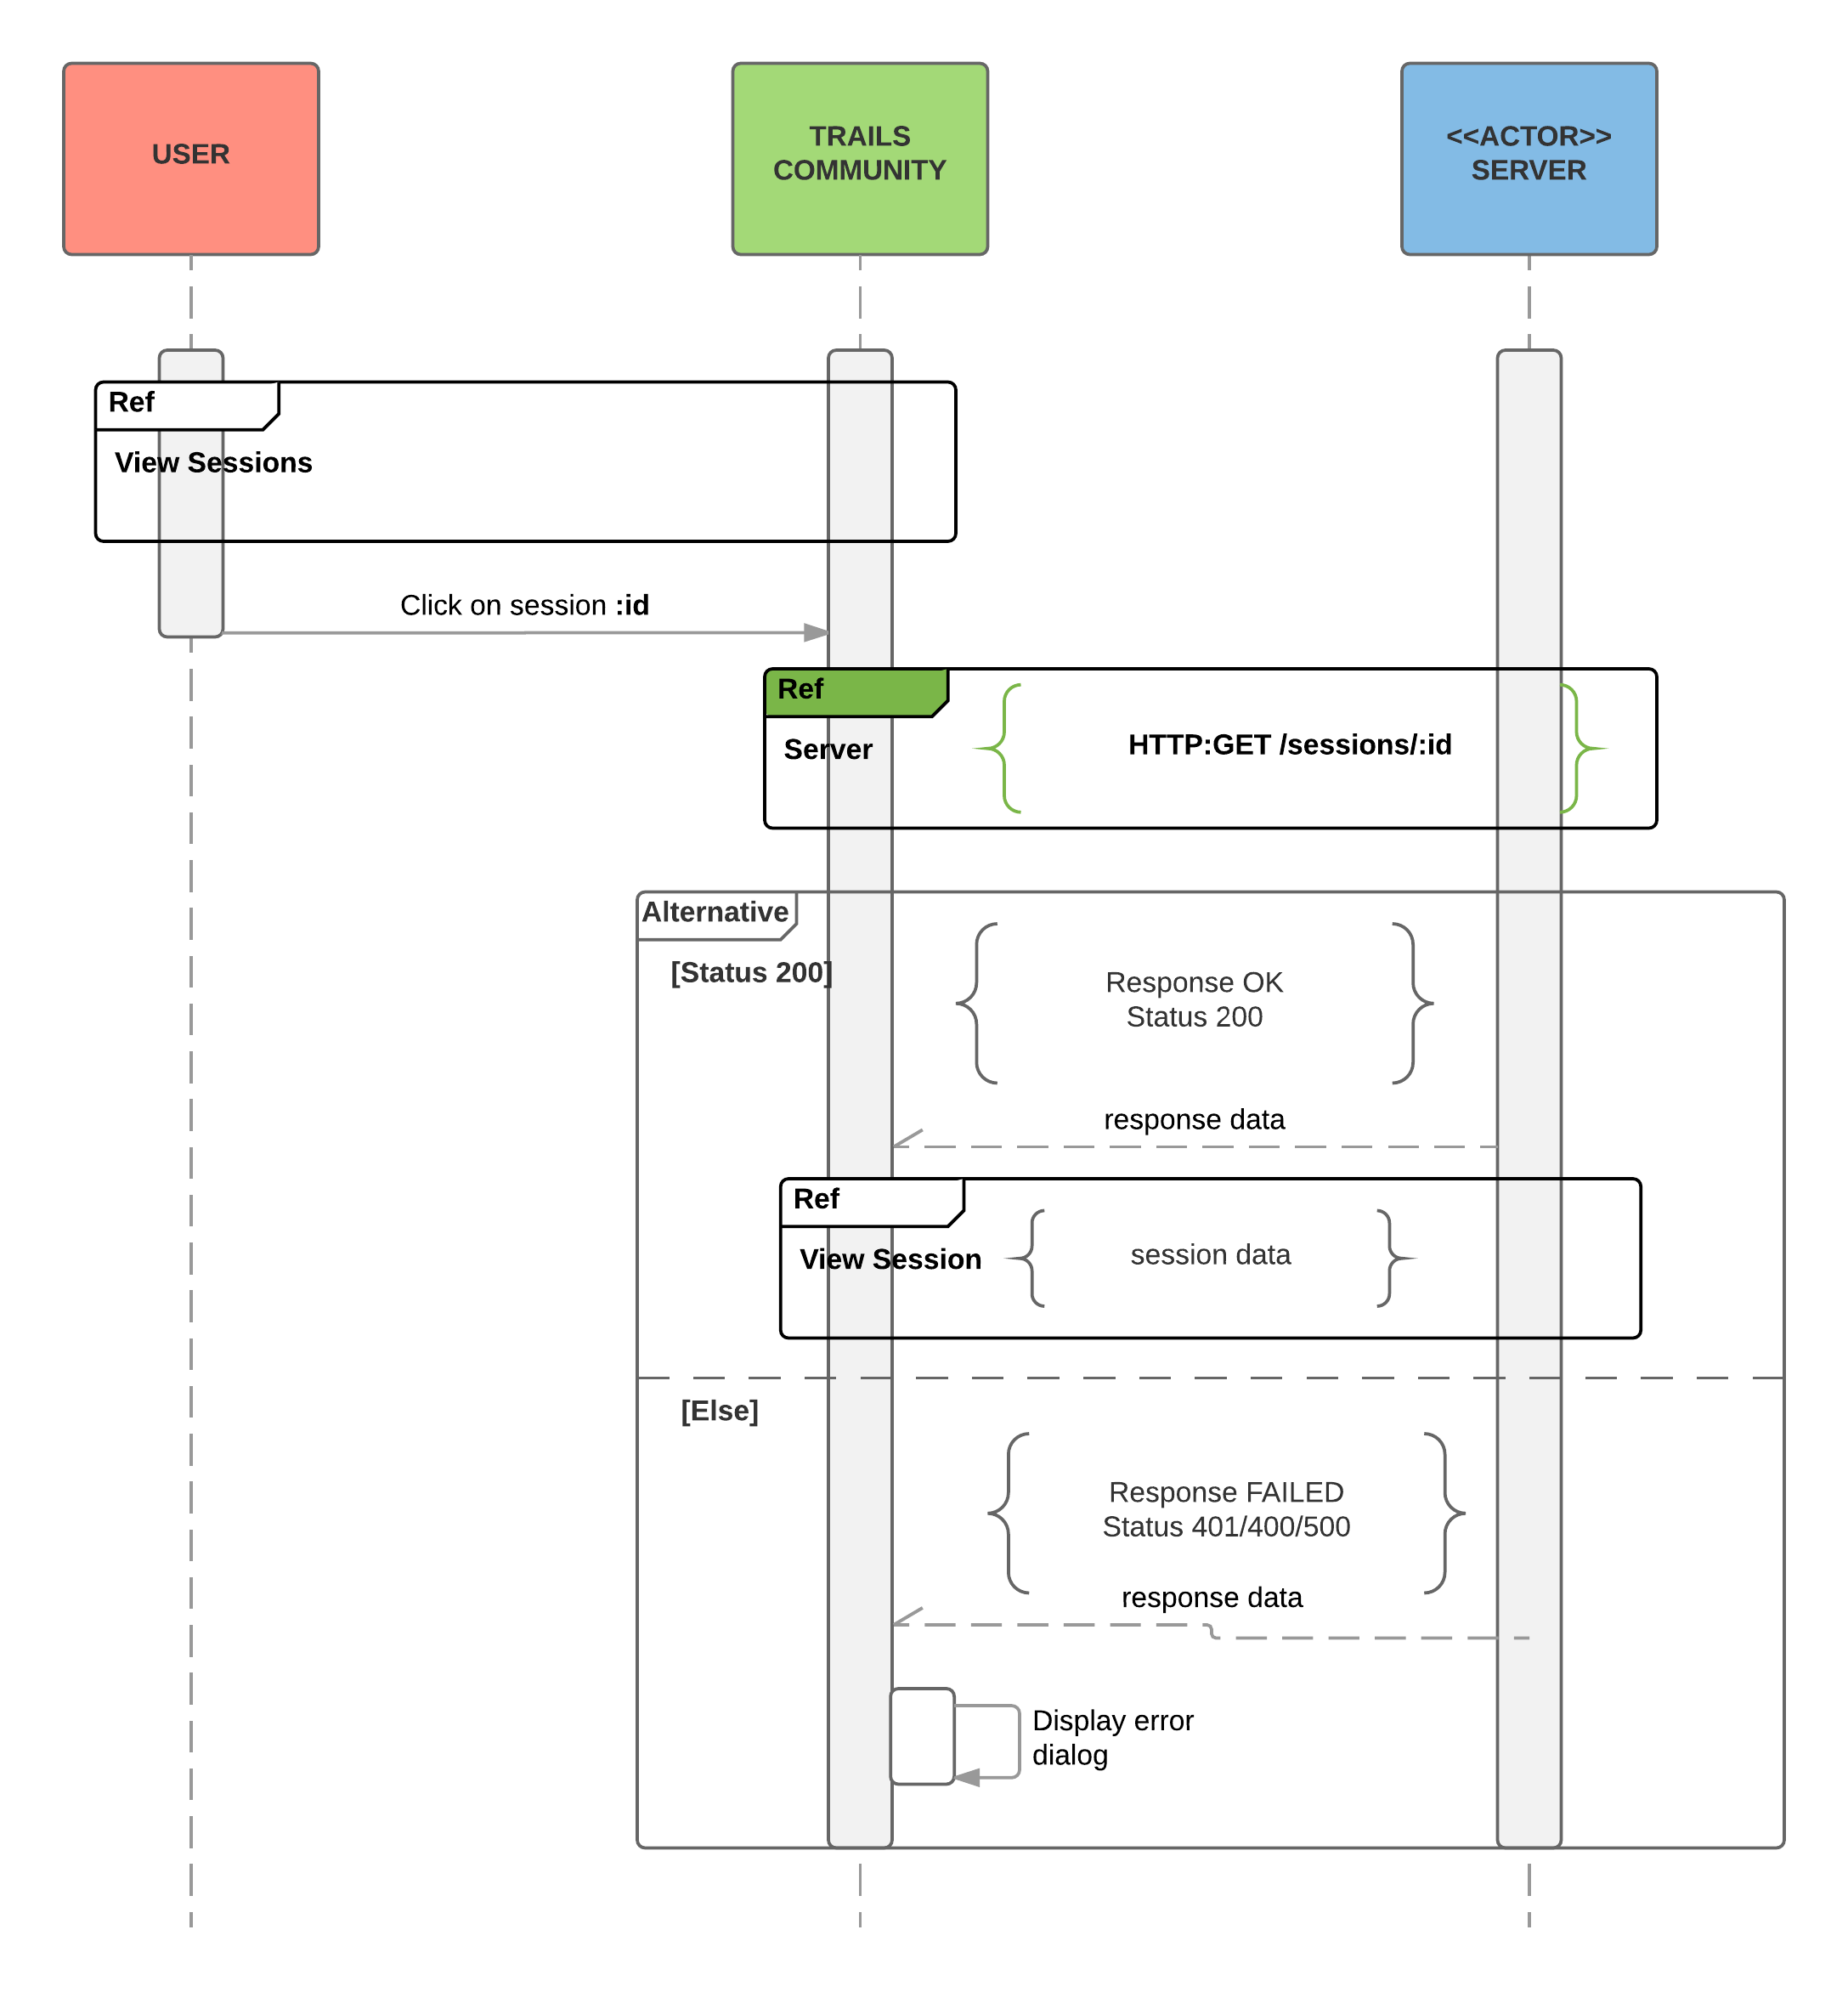
\includegraphics[scale=0.5]{Images/diagram/selection_session_sequence_diagram.png}
\end{figure}

\begin{figure}[!h]
	\caption{Diagramme de séquence pour l'affichage de l'ensemble des sessions}
	\label{view_sessions_sequence_diagram}
	\centering
	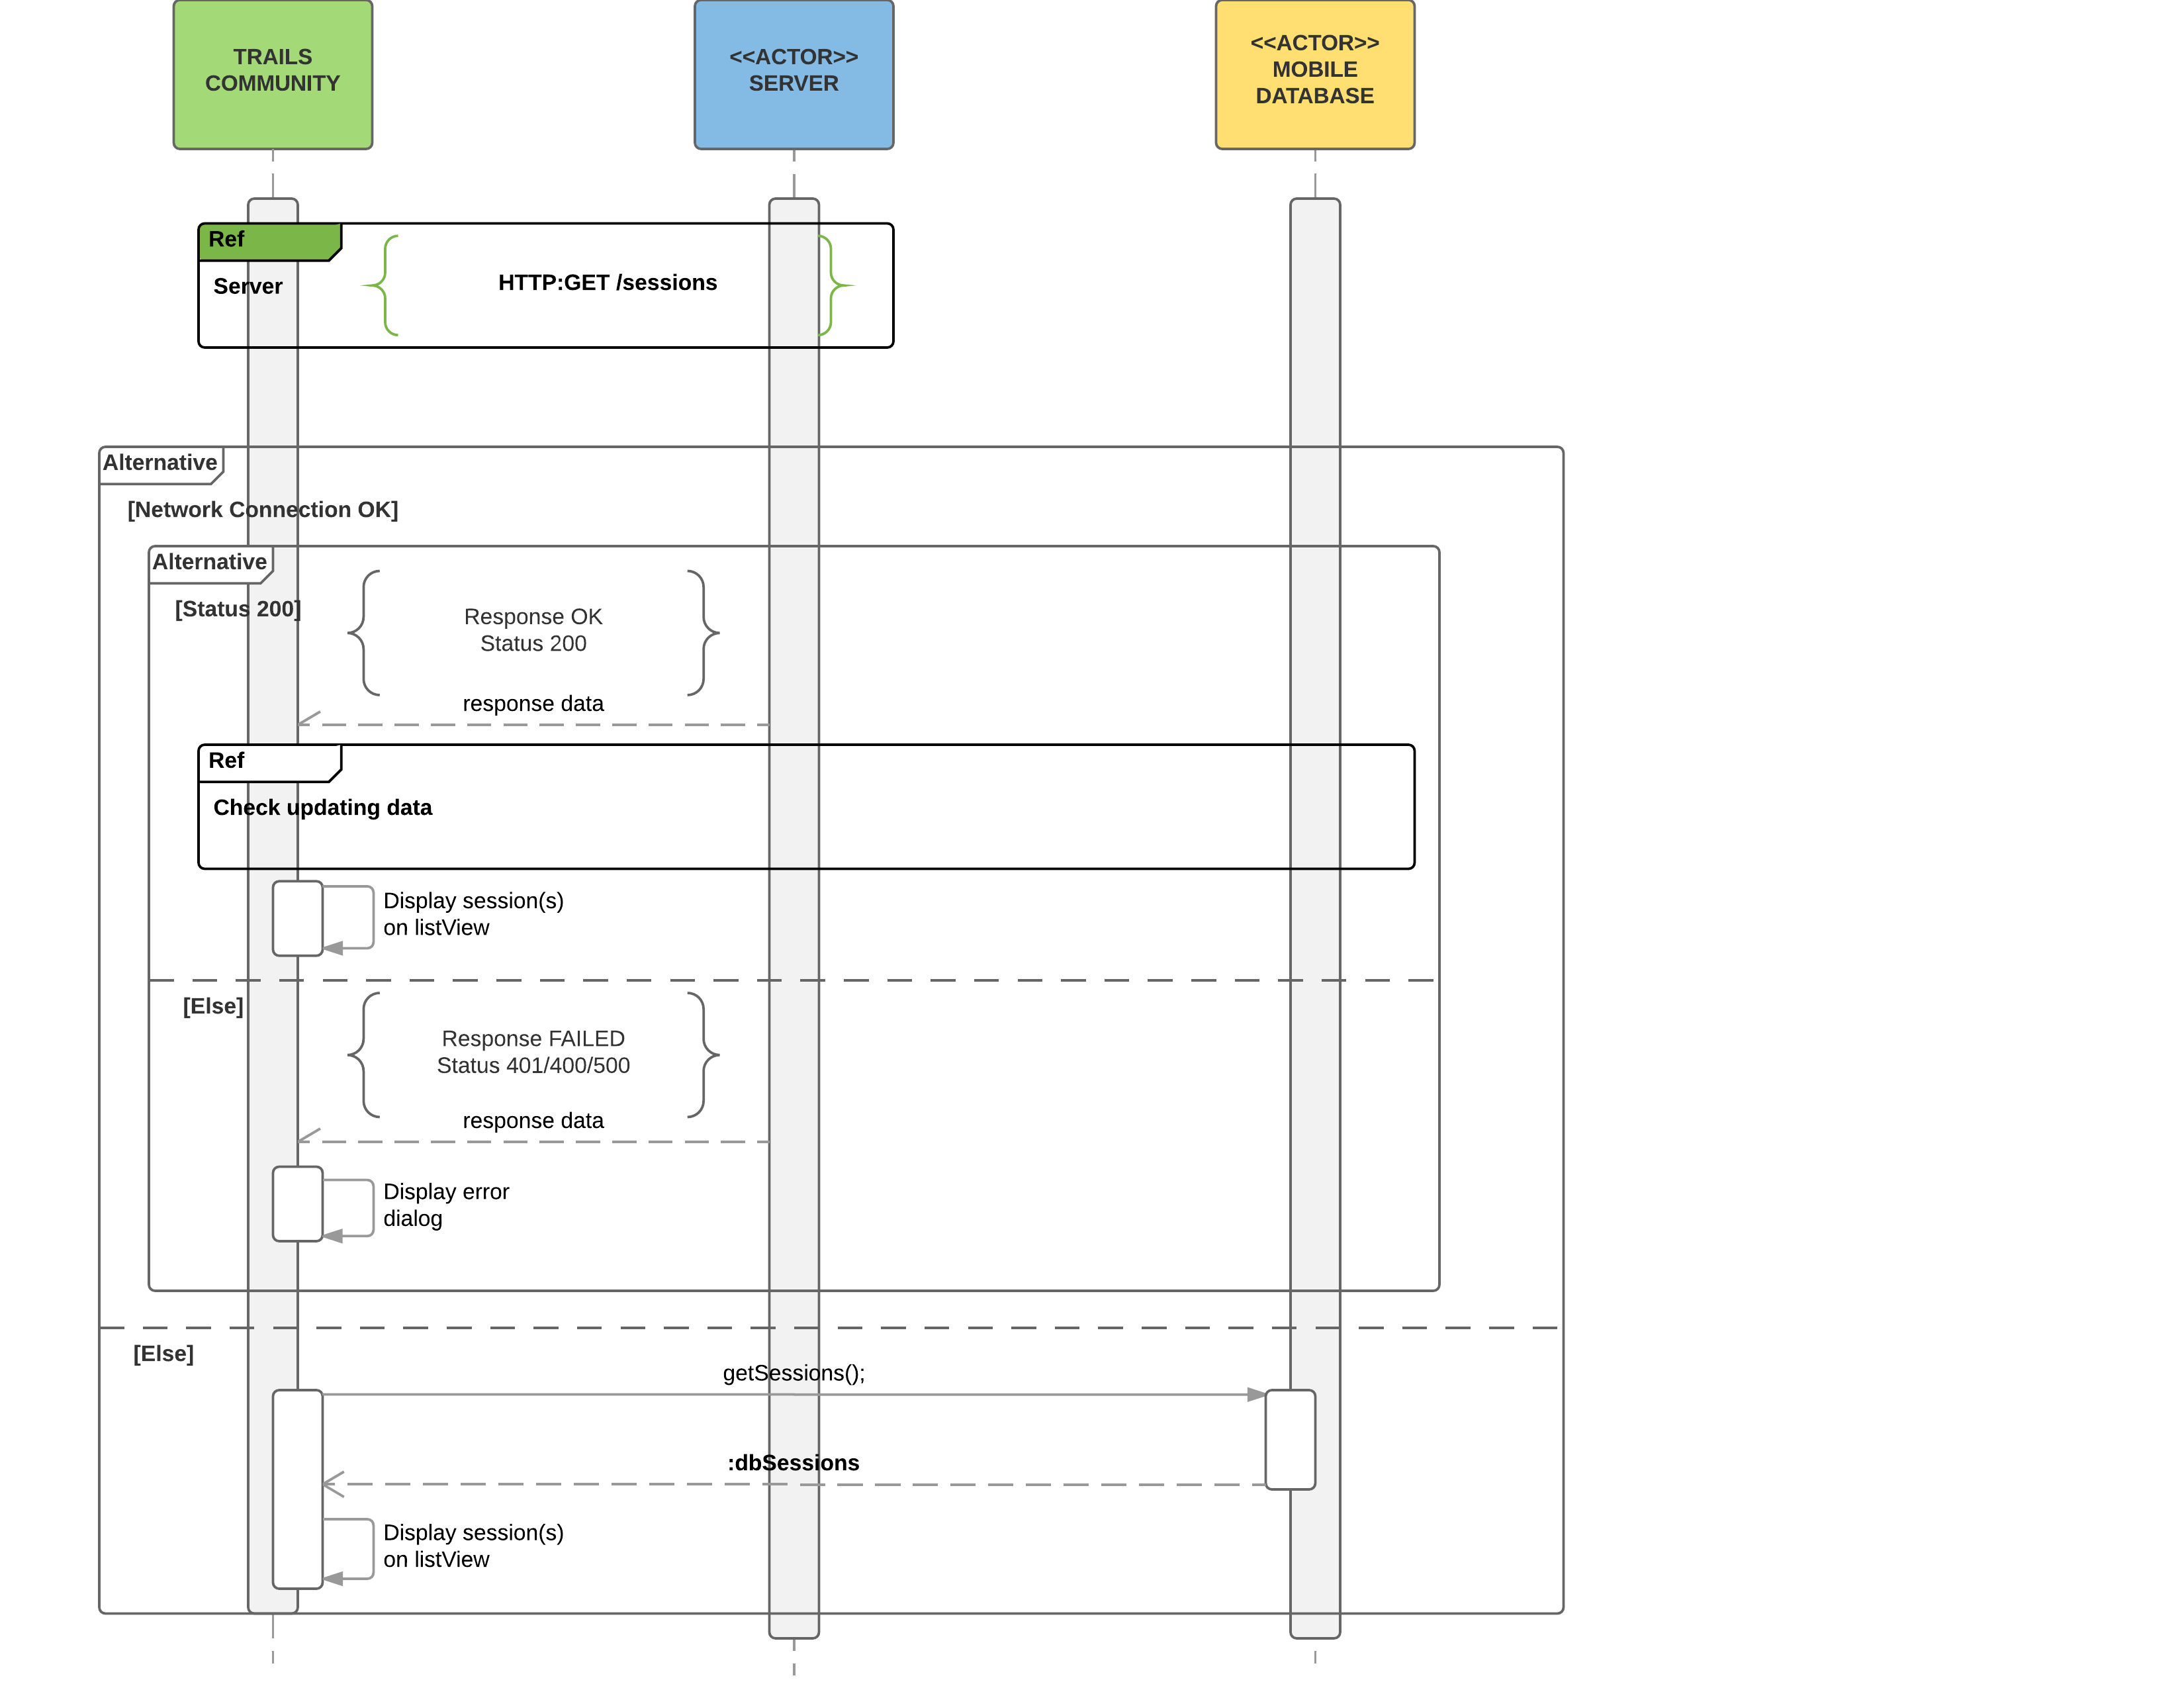
\includegraphics[scale=0.7]{Images/diagram/view_sessions_sequence_diagram.png}
\end{figure}

\chapter{Diagrammes d'activités}

\begin{figure}[!h]
	\caption{Diagramme d'activité de l'ajout d'un waypoint}
	\label{add_waypoint_activity_diagram}
	\centering
	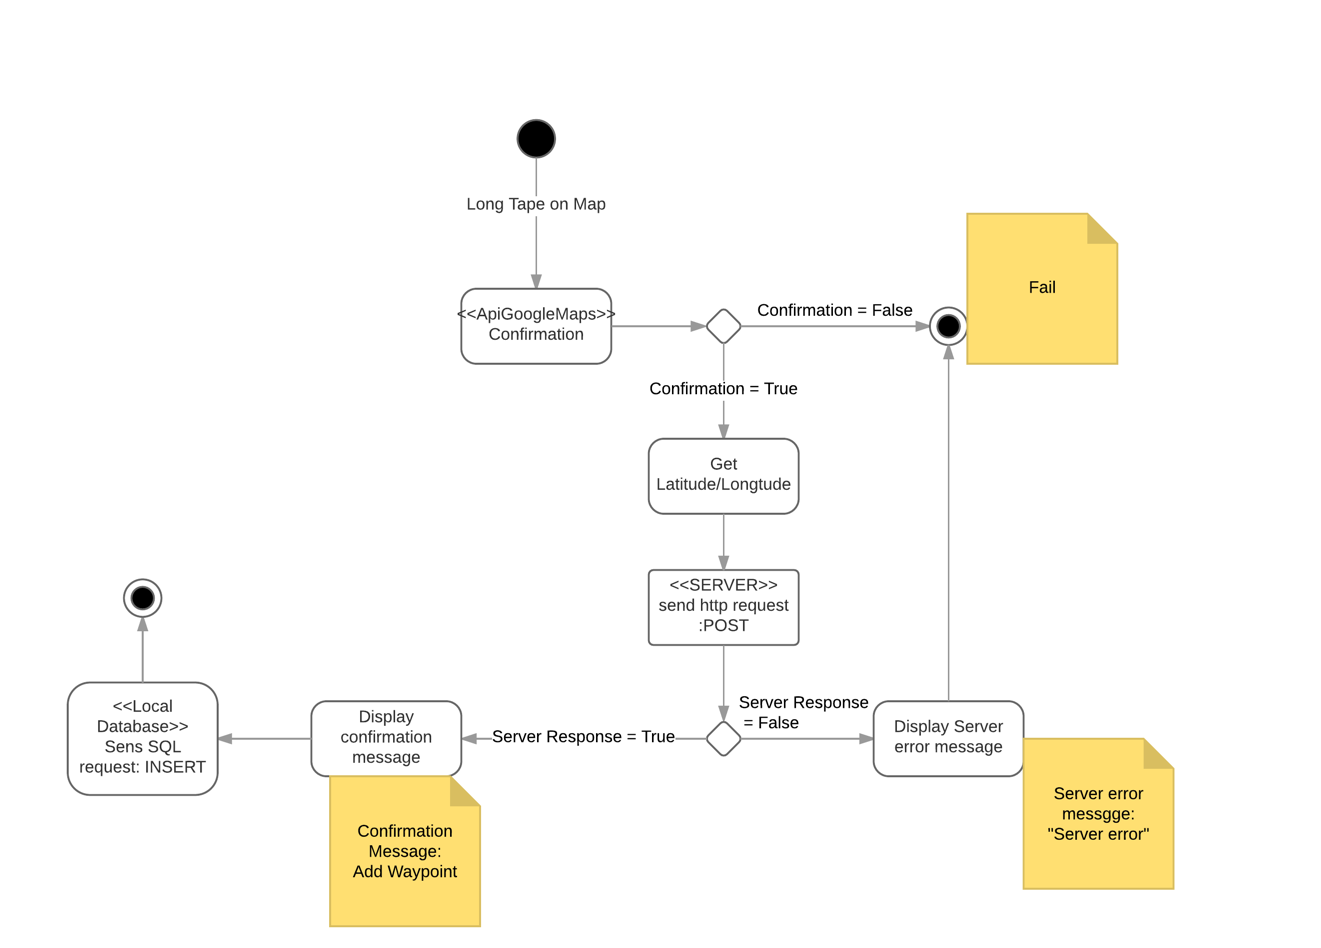
\includegraphics[scale=0.6]{Images/diagram/add_waypoint_activity_diagram.png}
\end{figure}

\begin{figure}[!h]
	\caption{Diagramme d'activité du chat}
	\label{chat_activity_diagram}
	\centering
	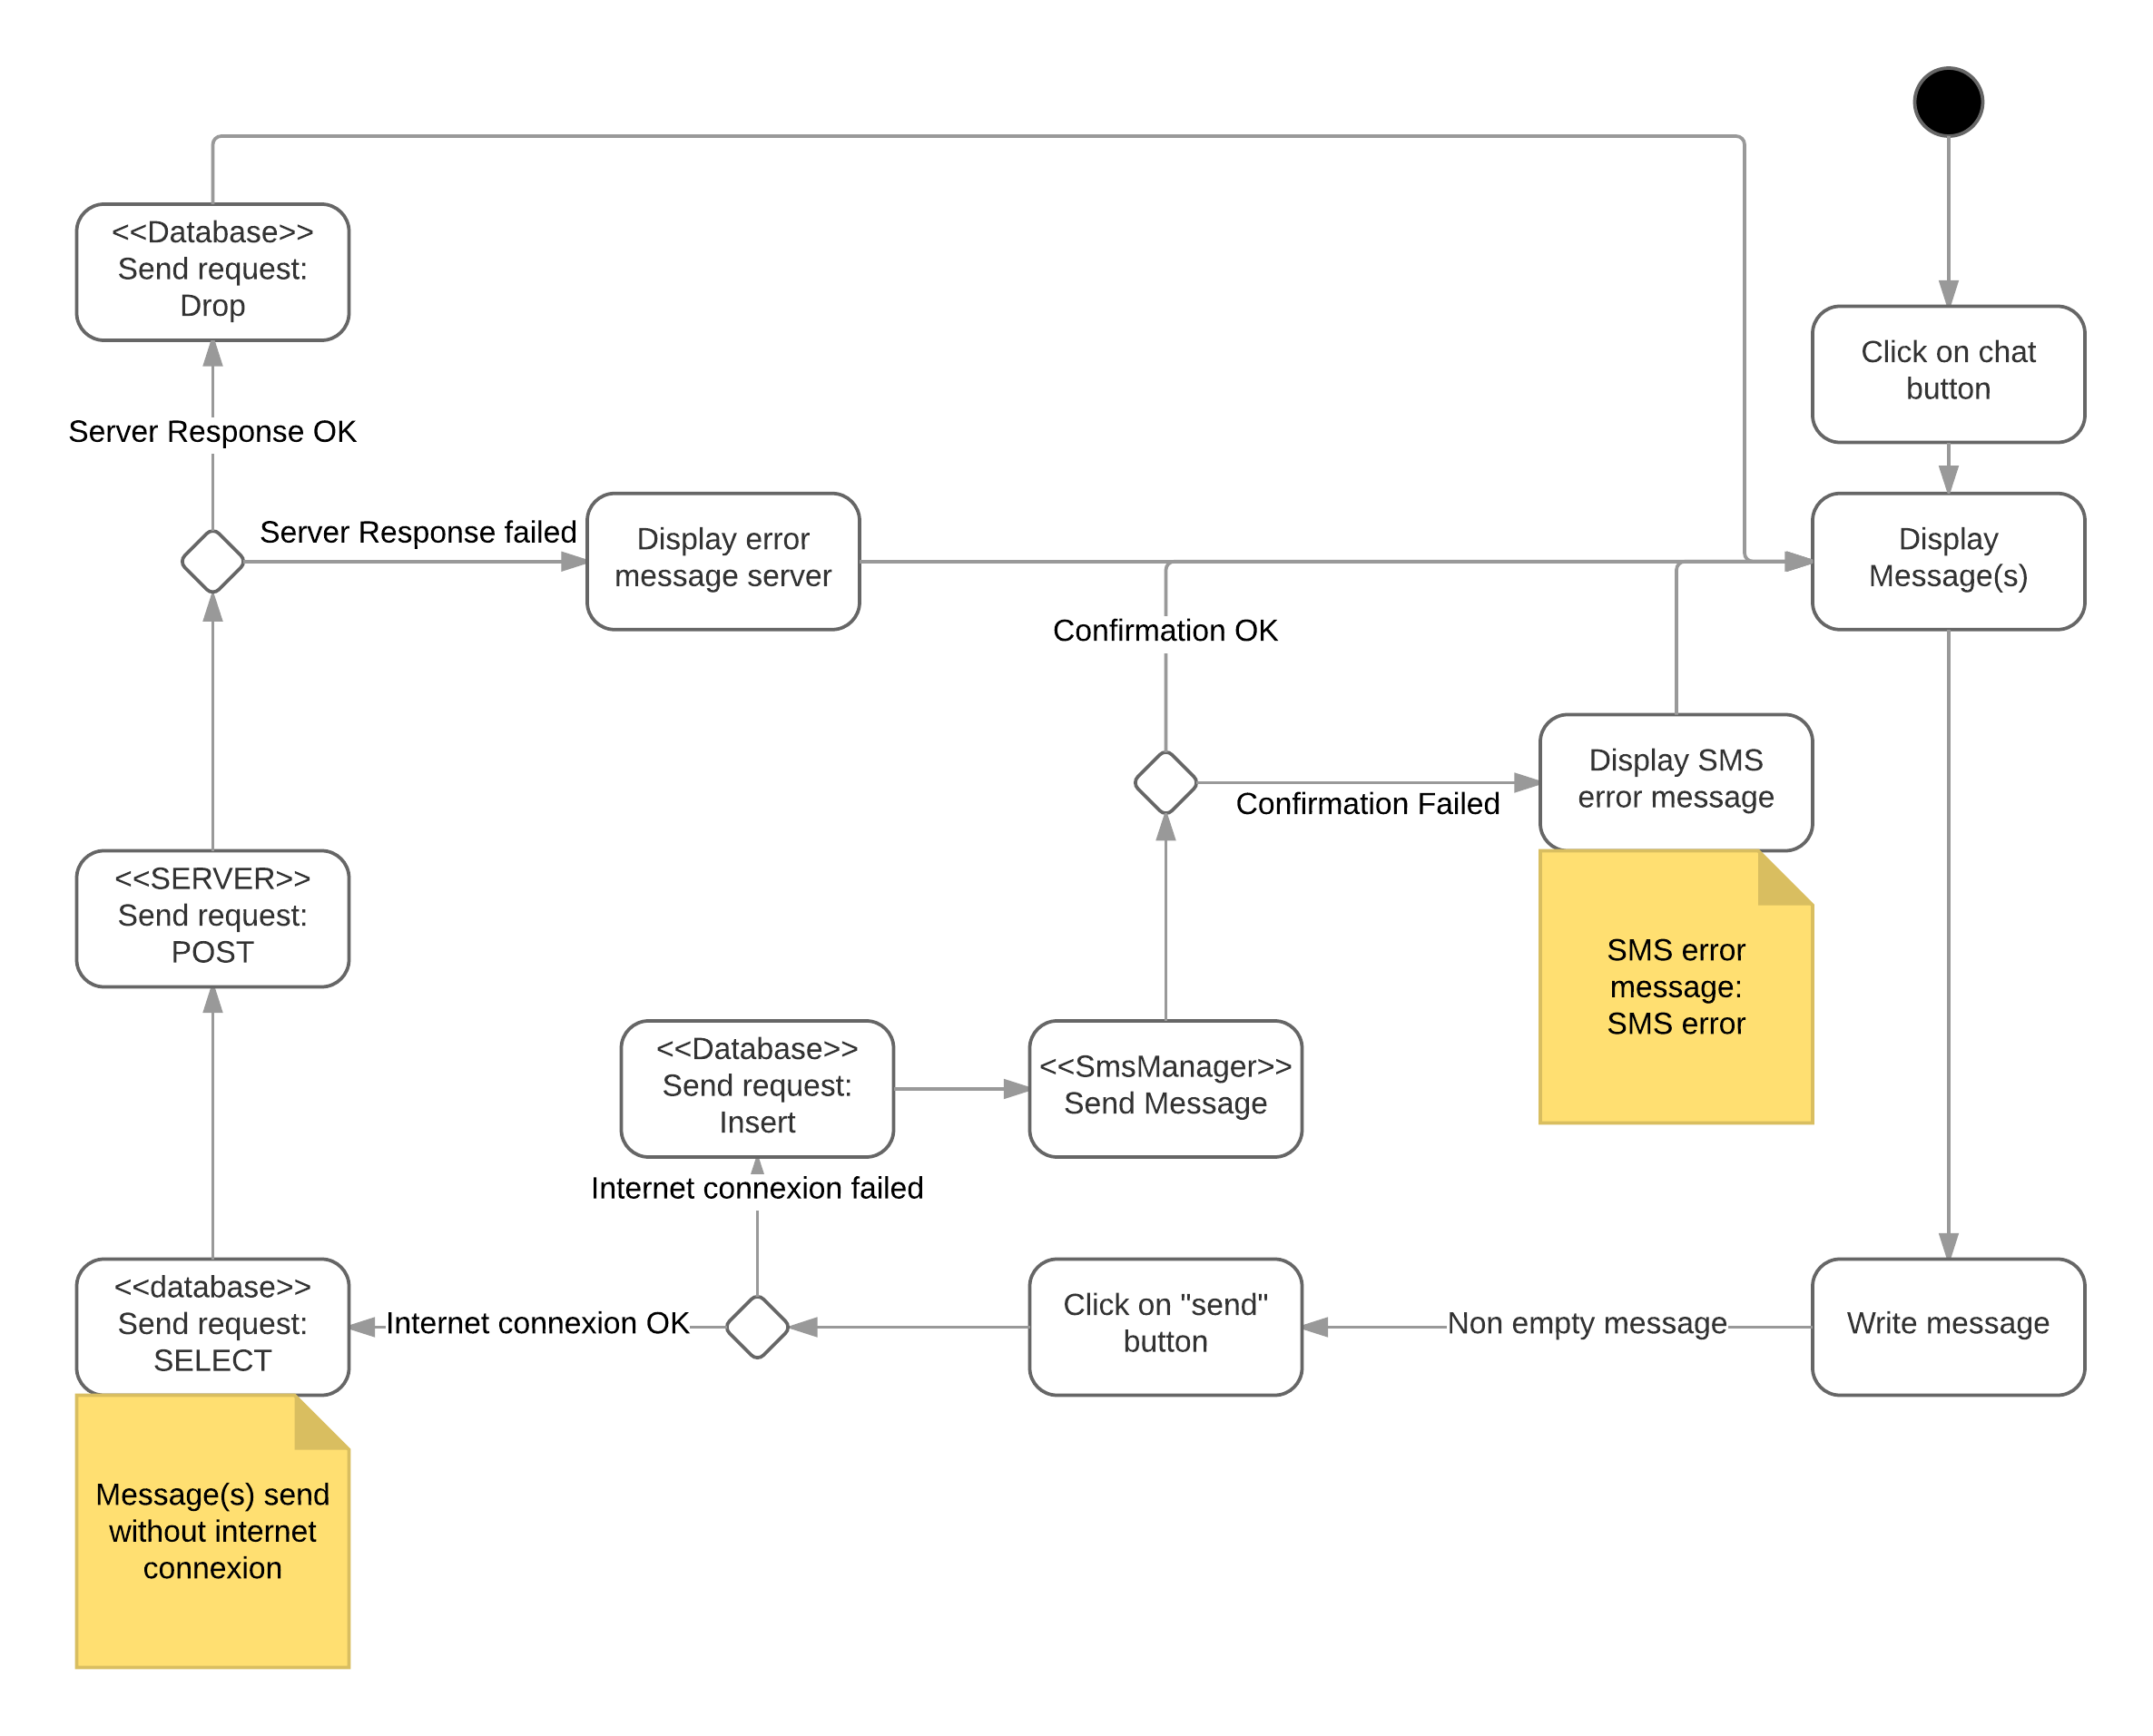
\includegraphics[scale=0.6]{Images/diagram/chat_activity_diagram.png}
\end{figure}  

\begin{figure}[!h]
	\caption{Diagramme d'activité pour l'authentification}
	\label{login_activity_diagram}
	\centering
	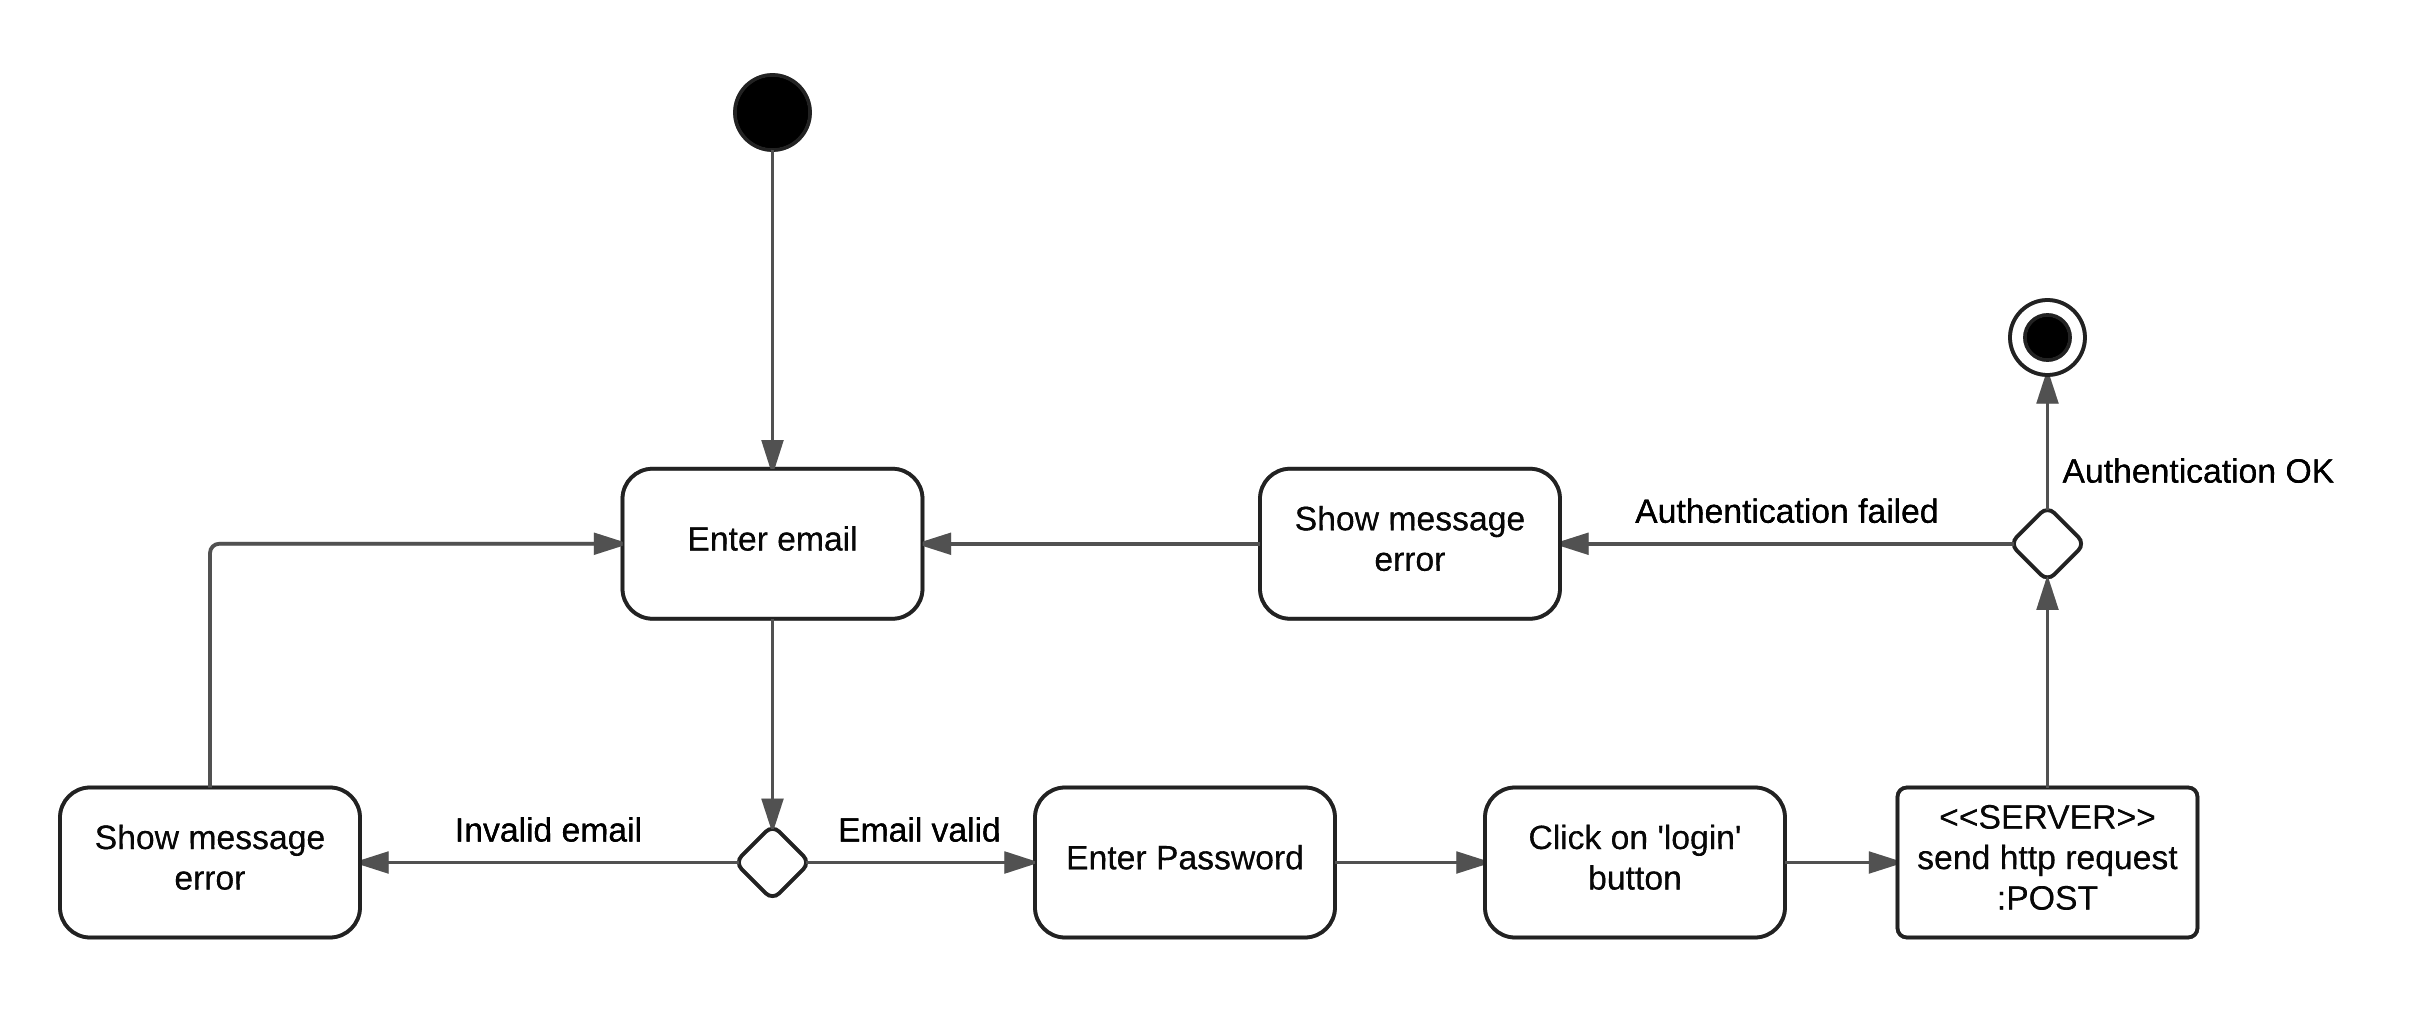
\includegraphics[scale=0.6]{Images/diagram/login_activity_diagram.png}
\end{figure} 

\begin{figure}[!h]
	\caption{Diagramme d'activité pour la modification du profile}
	\label{modify_profil_activity_diagram}
	\centering
	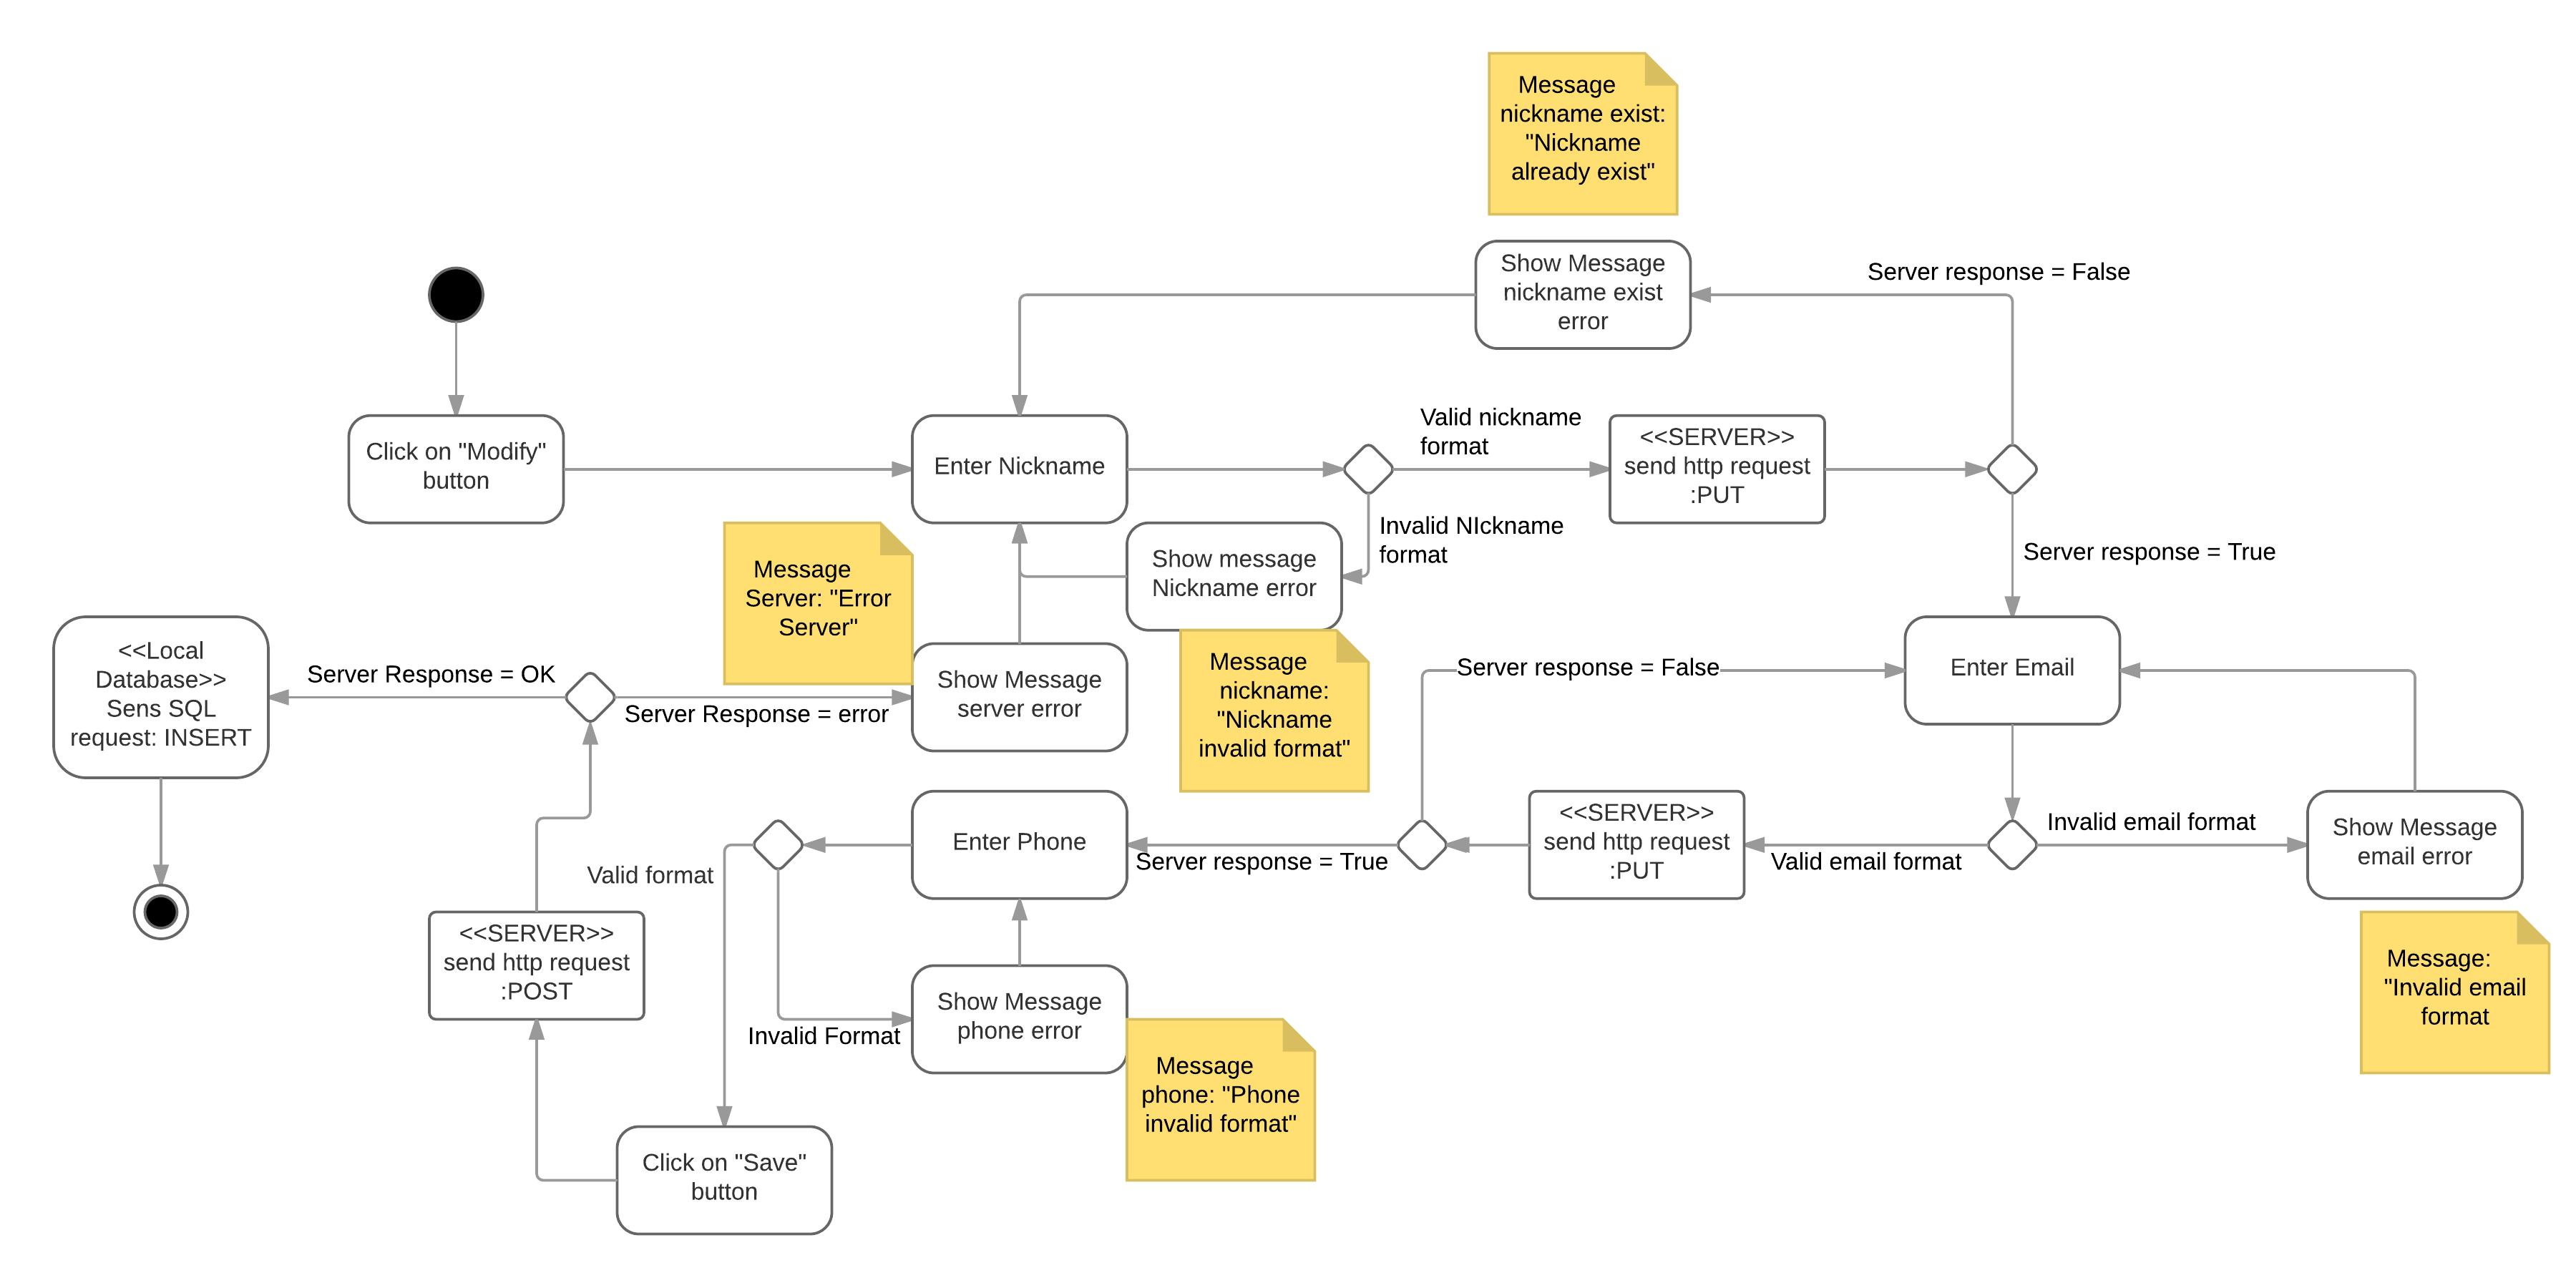
\includegraphics[scale=0.6]{Images/diagram/modify_profil_activity_diagram.png}
\end{figure} 

\begin{figure}[!h]
	\caption{Diagramme d'activité pour la sélection d'une session}
	\label{selection_session_activity_diagram}
	\centering
	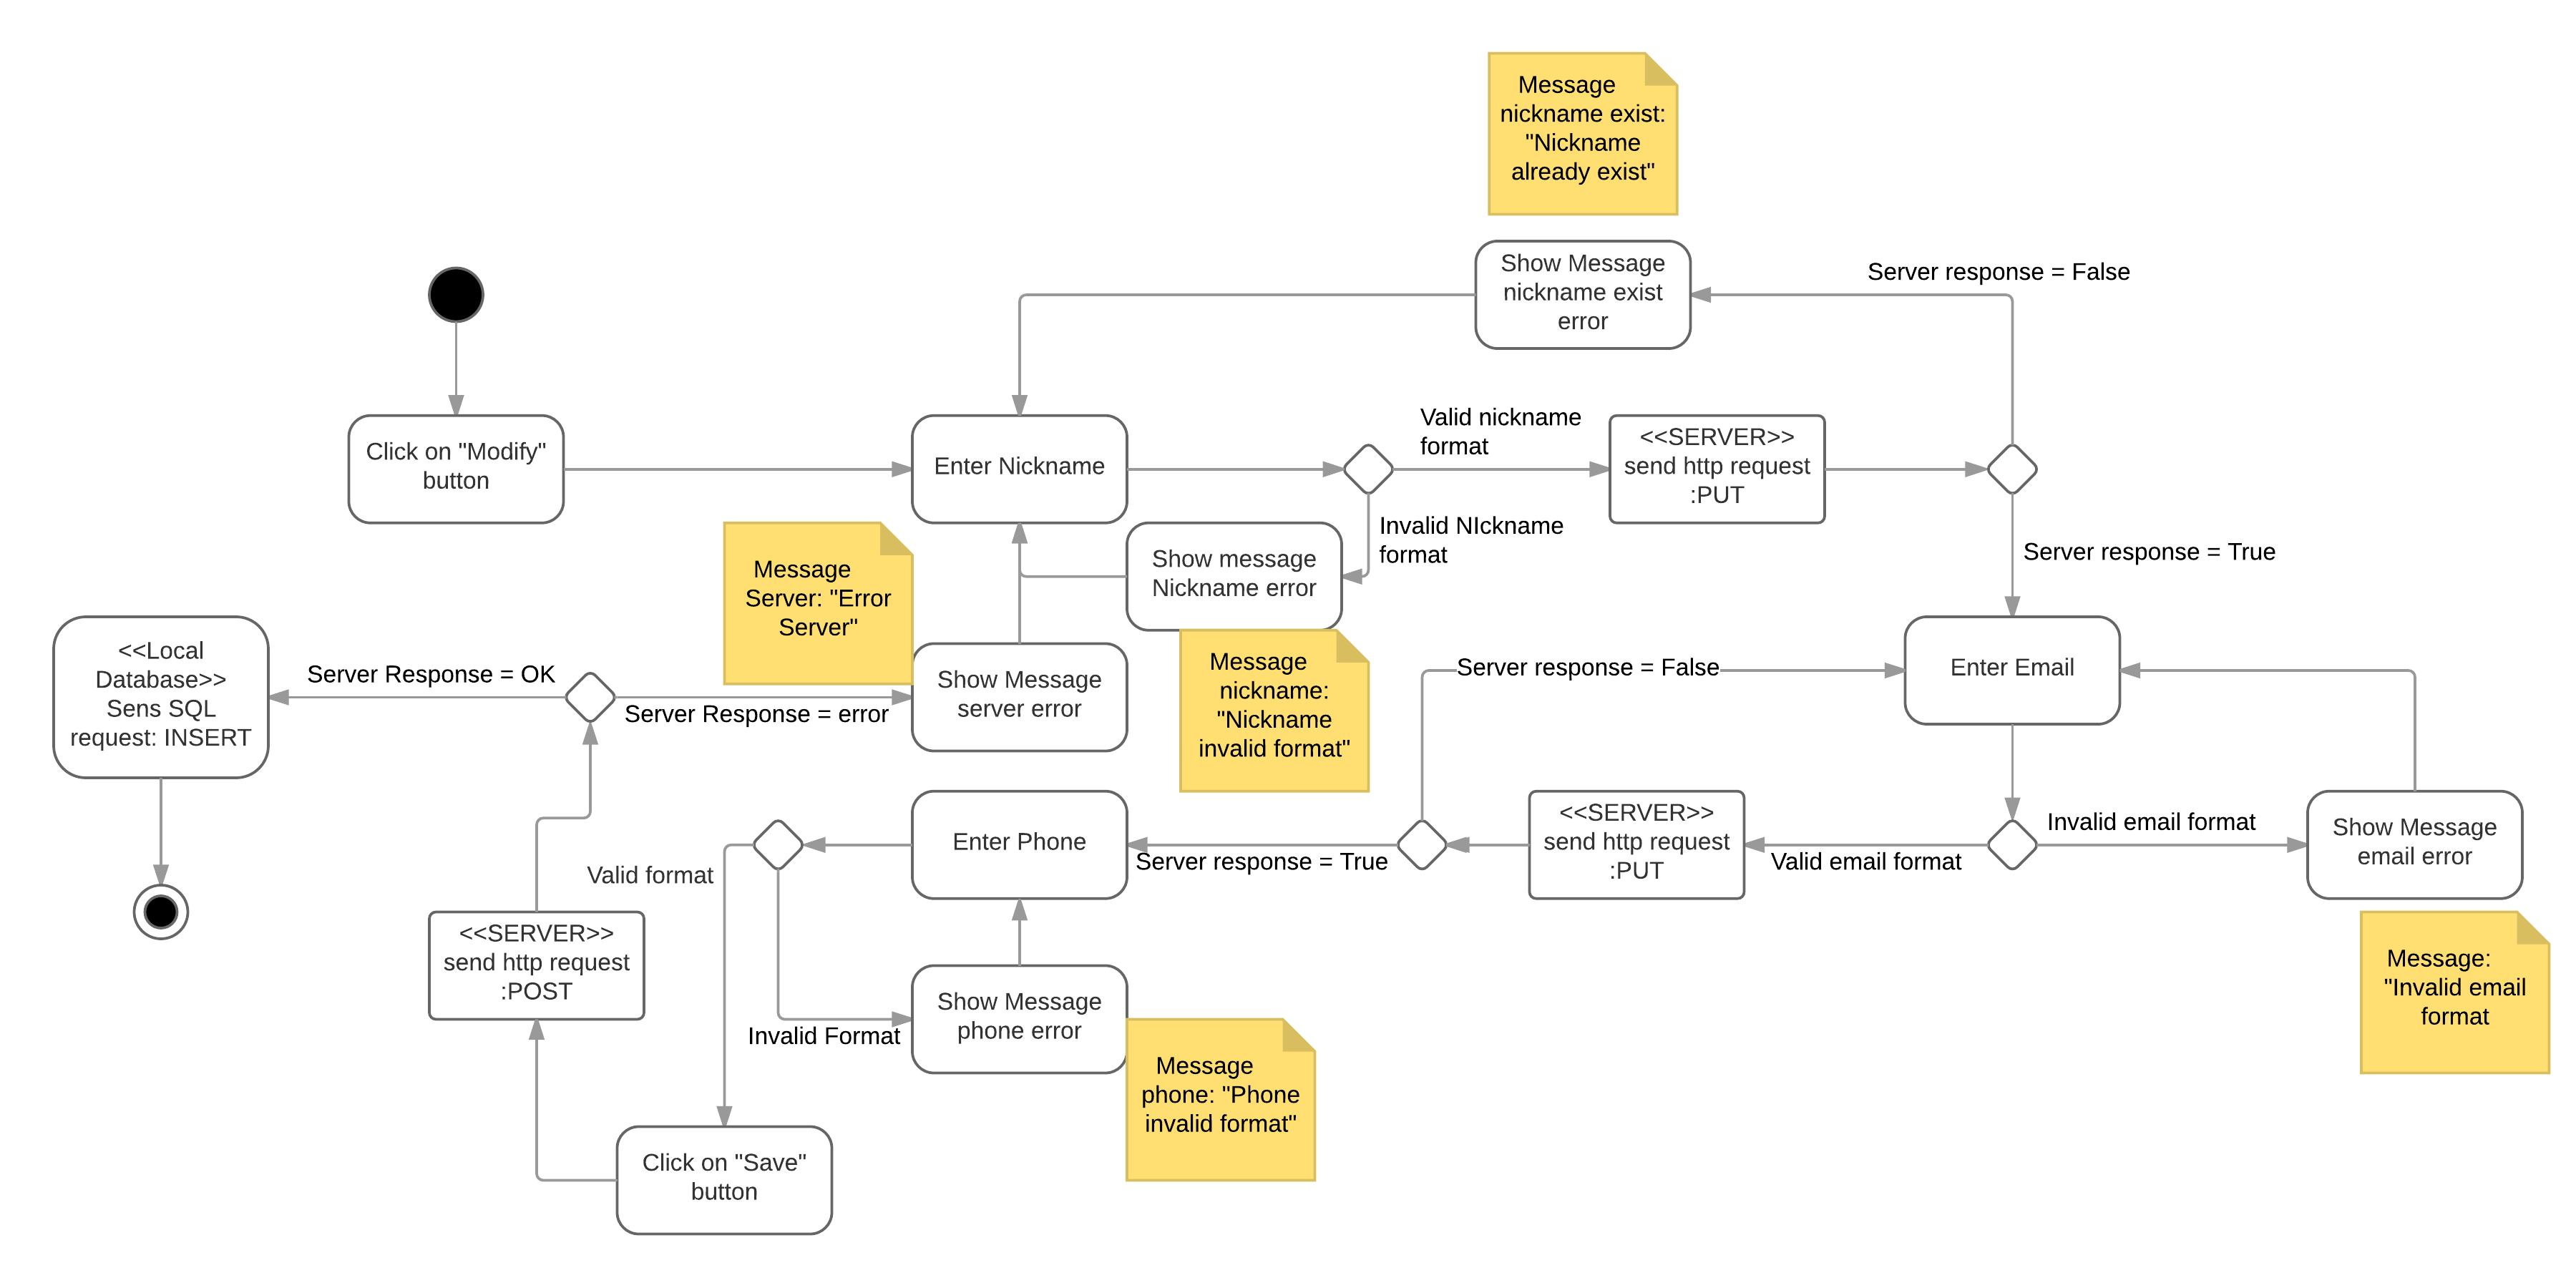
\includegraphics[scale=0.6]{Images/diagram/modify_profil_activity_diagram.png}
\end{figure}

\begin{figure}[!h]
	\caption{Diagramme d'activité pour l'utilisation de la géolocalisation}
	\label{use_geolocalistion_activity_diagram}
	\centering
	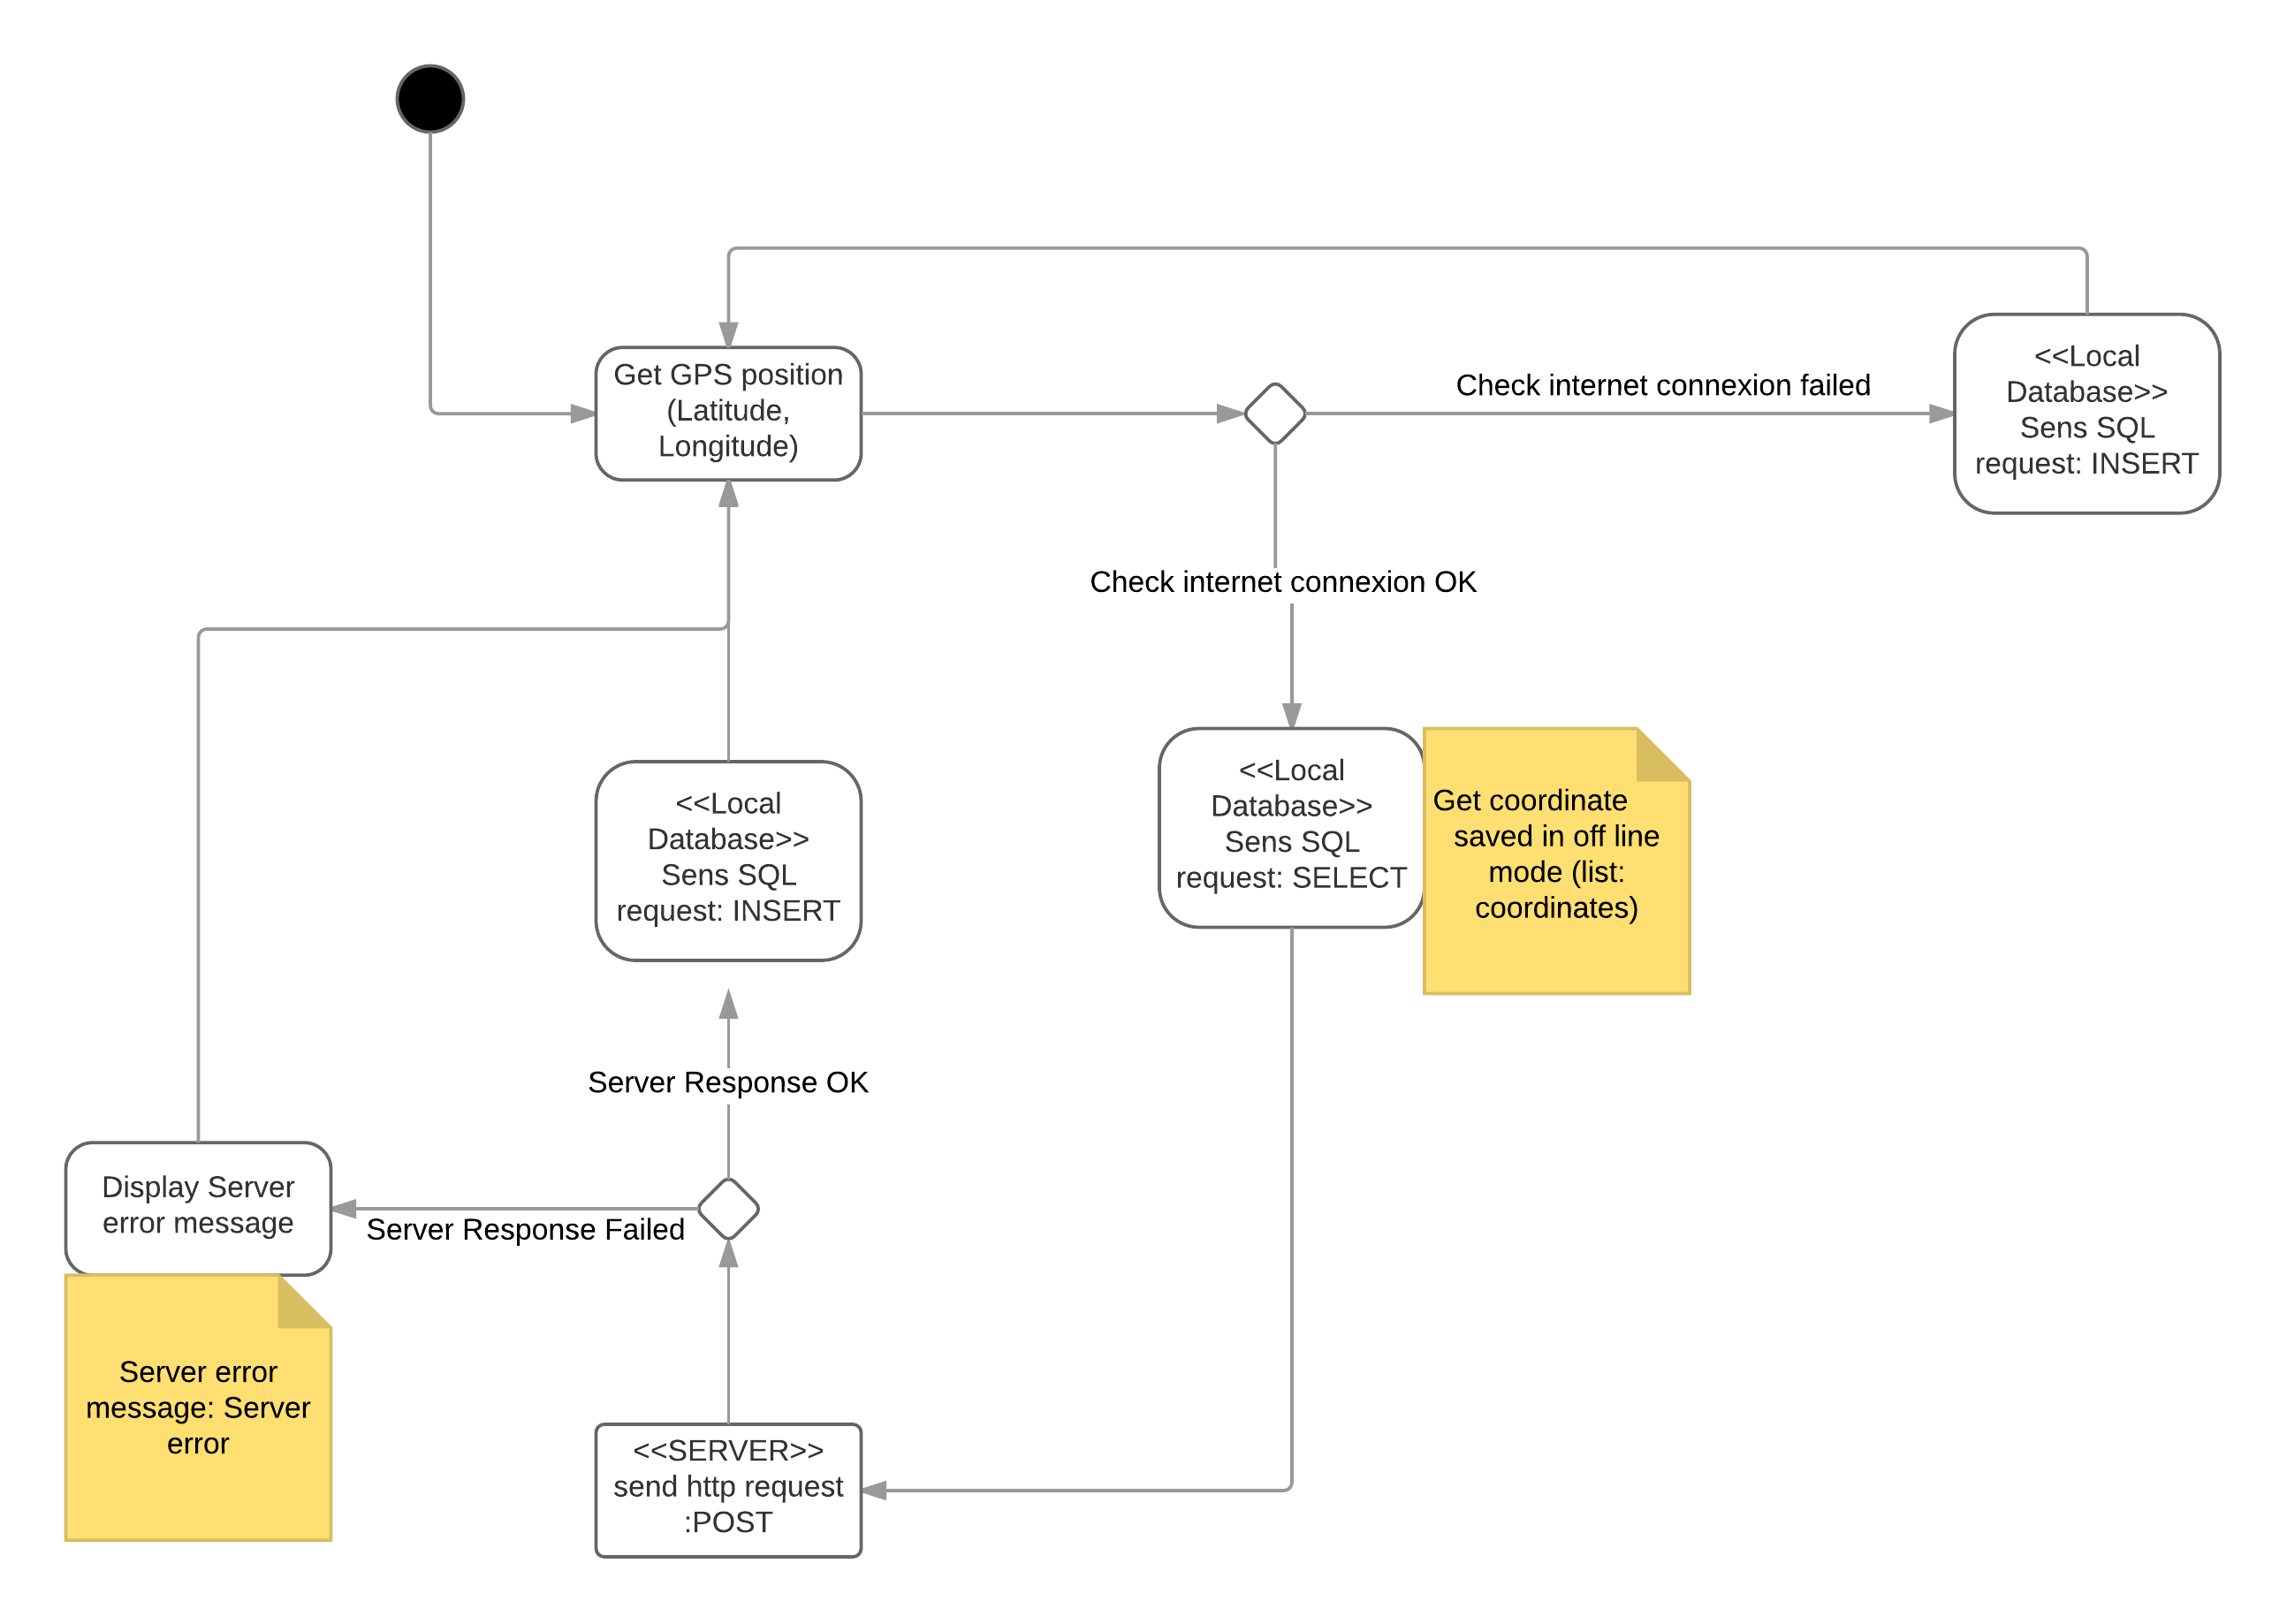
\includegraphics[scale=0.6]{Images/diagram/use_geolocalisation_activity_diagram.png}
\end{figure}

\begin{figure}[!h]
	\caption{Diagramme d'activité pour l'affichage de l'ensemble des sessions}
	\label{view_sessions_activity_diagram}
	\centering
	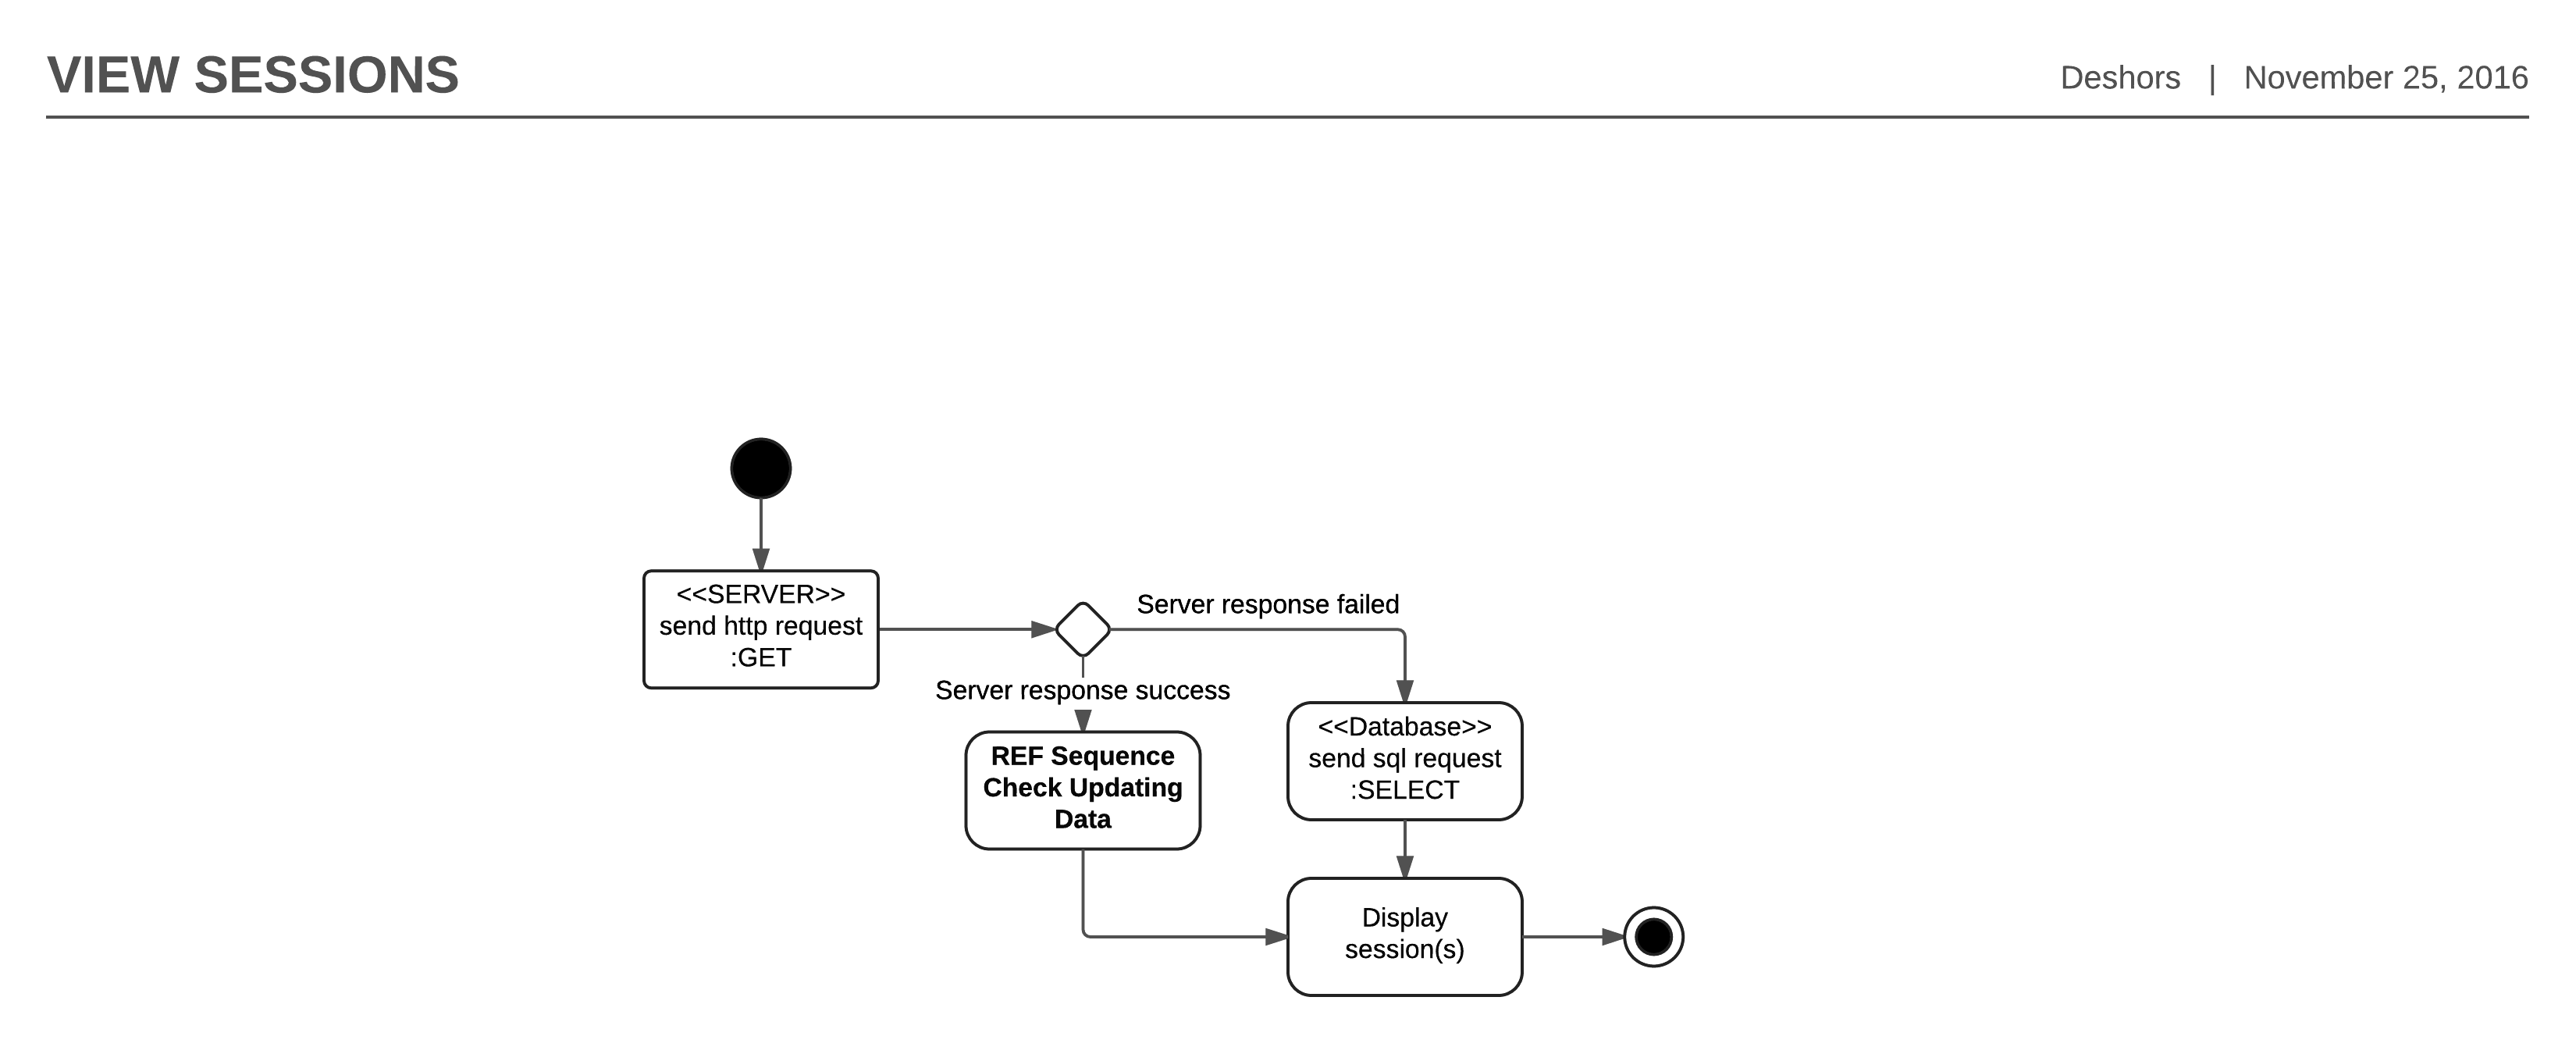
\includegraphics[scale=0.6]{Images/diagram/view_sessions_activity_diagram.png}
\end{figure}

\chapter{Diagrammes d'états}  

\begin{figure}[!h]
	\caption{Diagramme d'état d'un acteur}
	\label{state_actor_diagram}
	\centering
	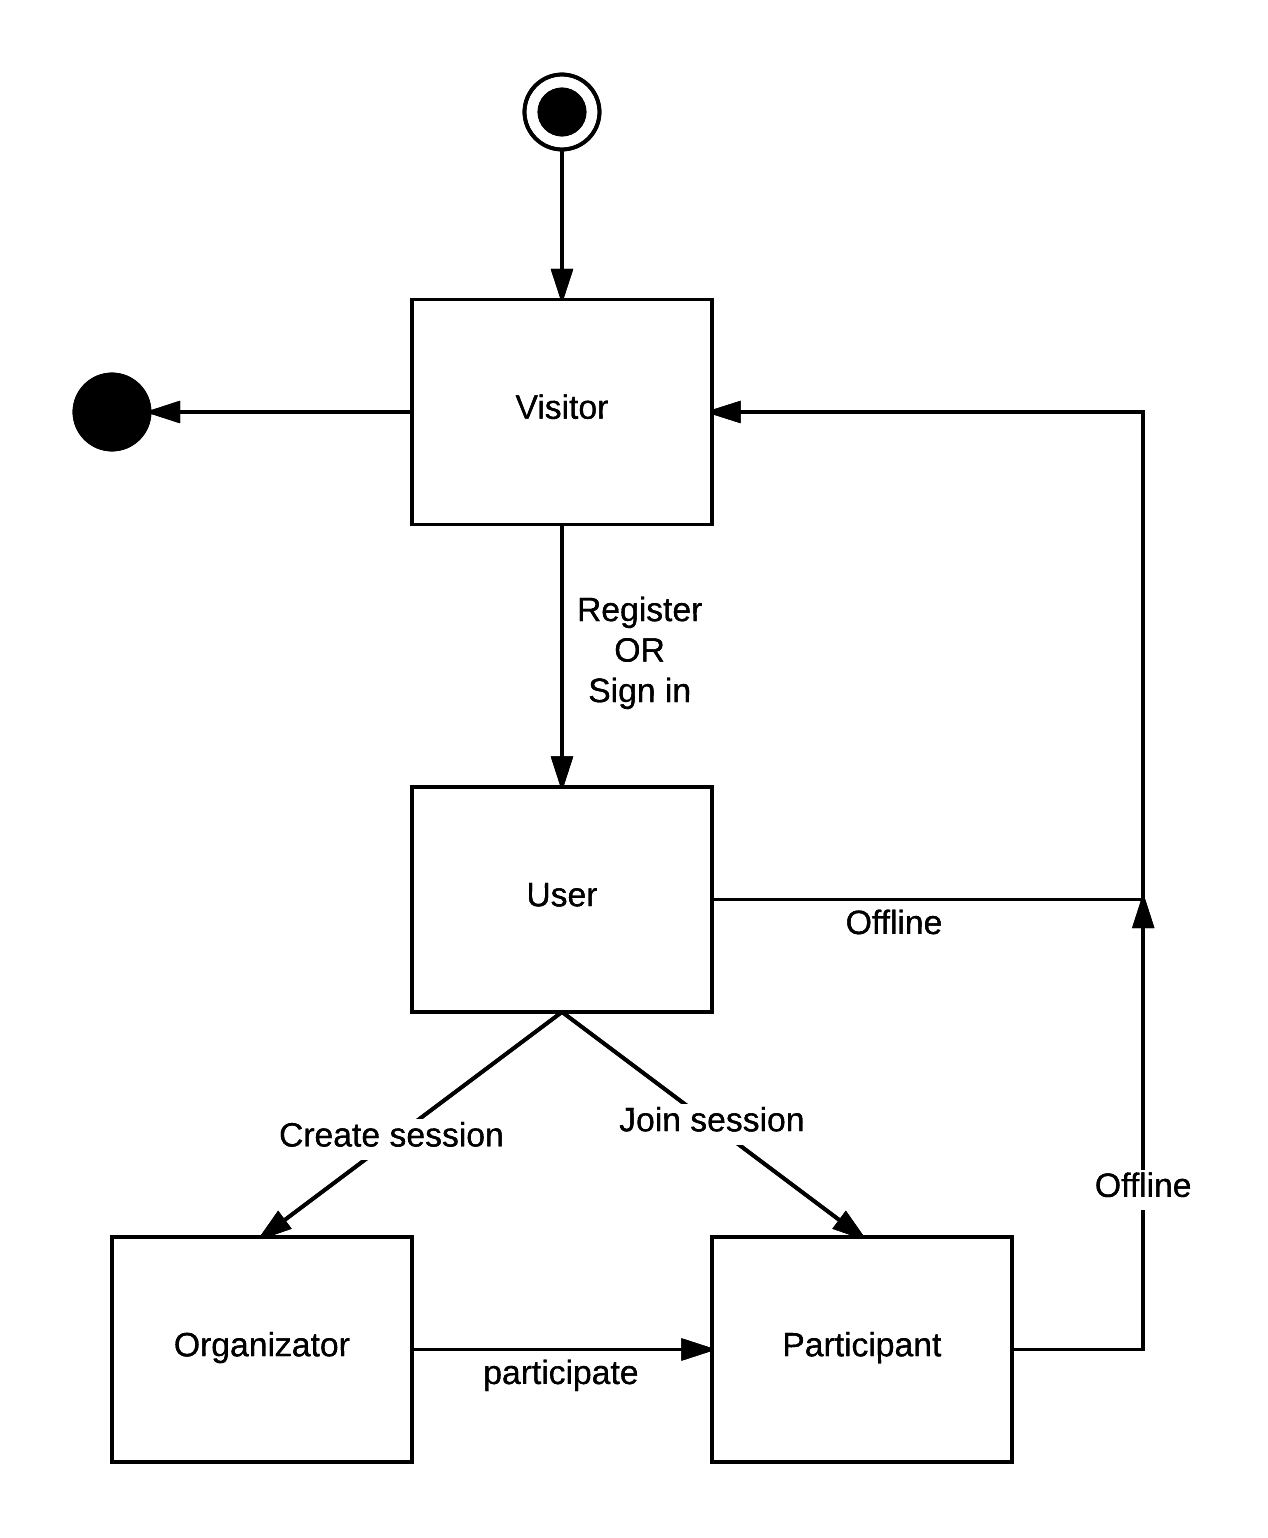
\includegraphics[scale=0.8]{Images/diagram/state_actor_diagram.png}
\end{figure}

\begin{figure}[!h]
	\caption{Diagramme d'état d'une session}
	\label{state_session_diagram}
	\centering
	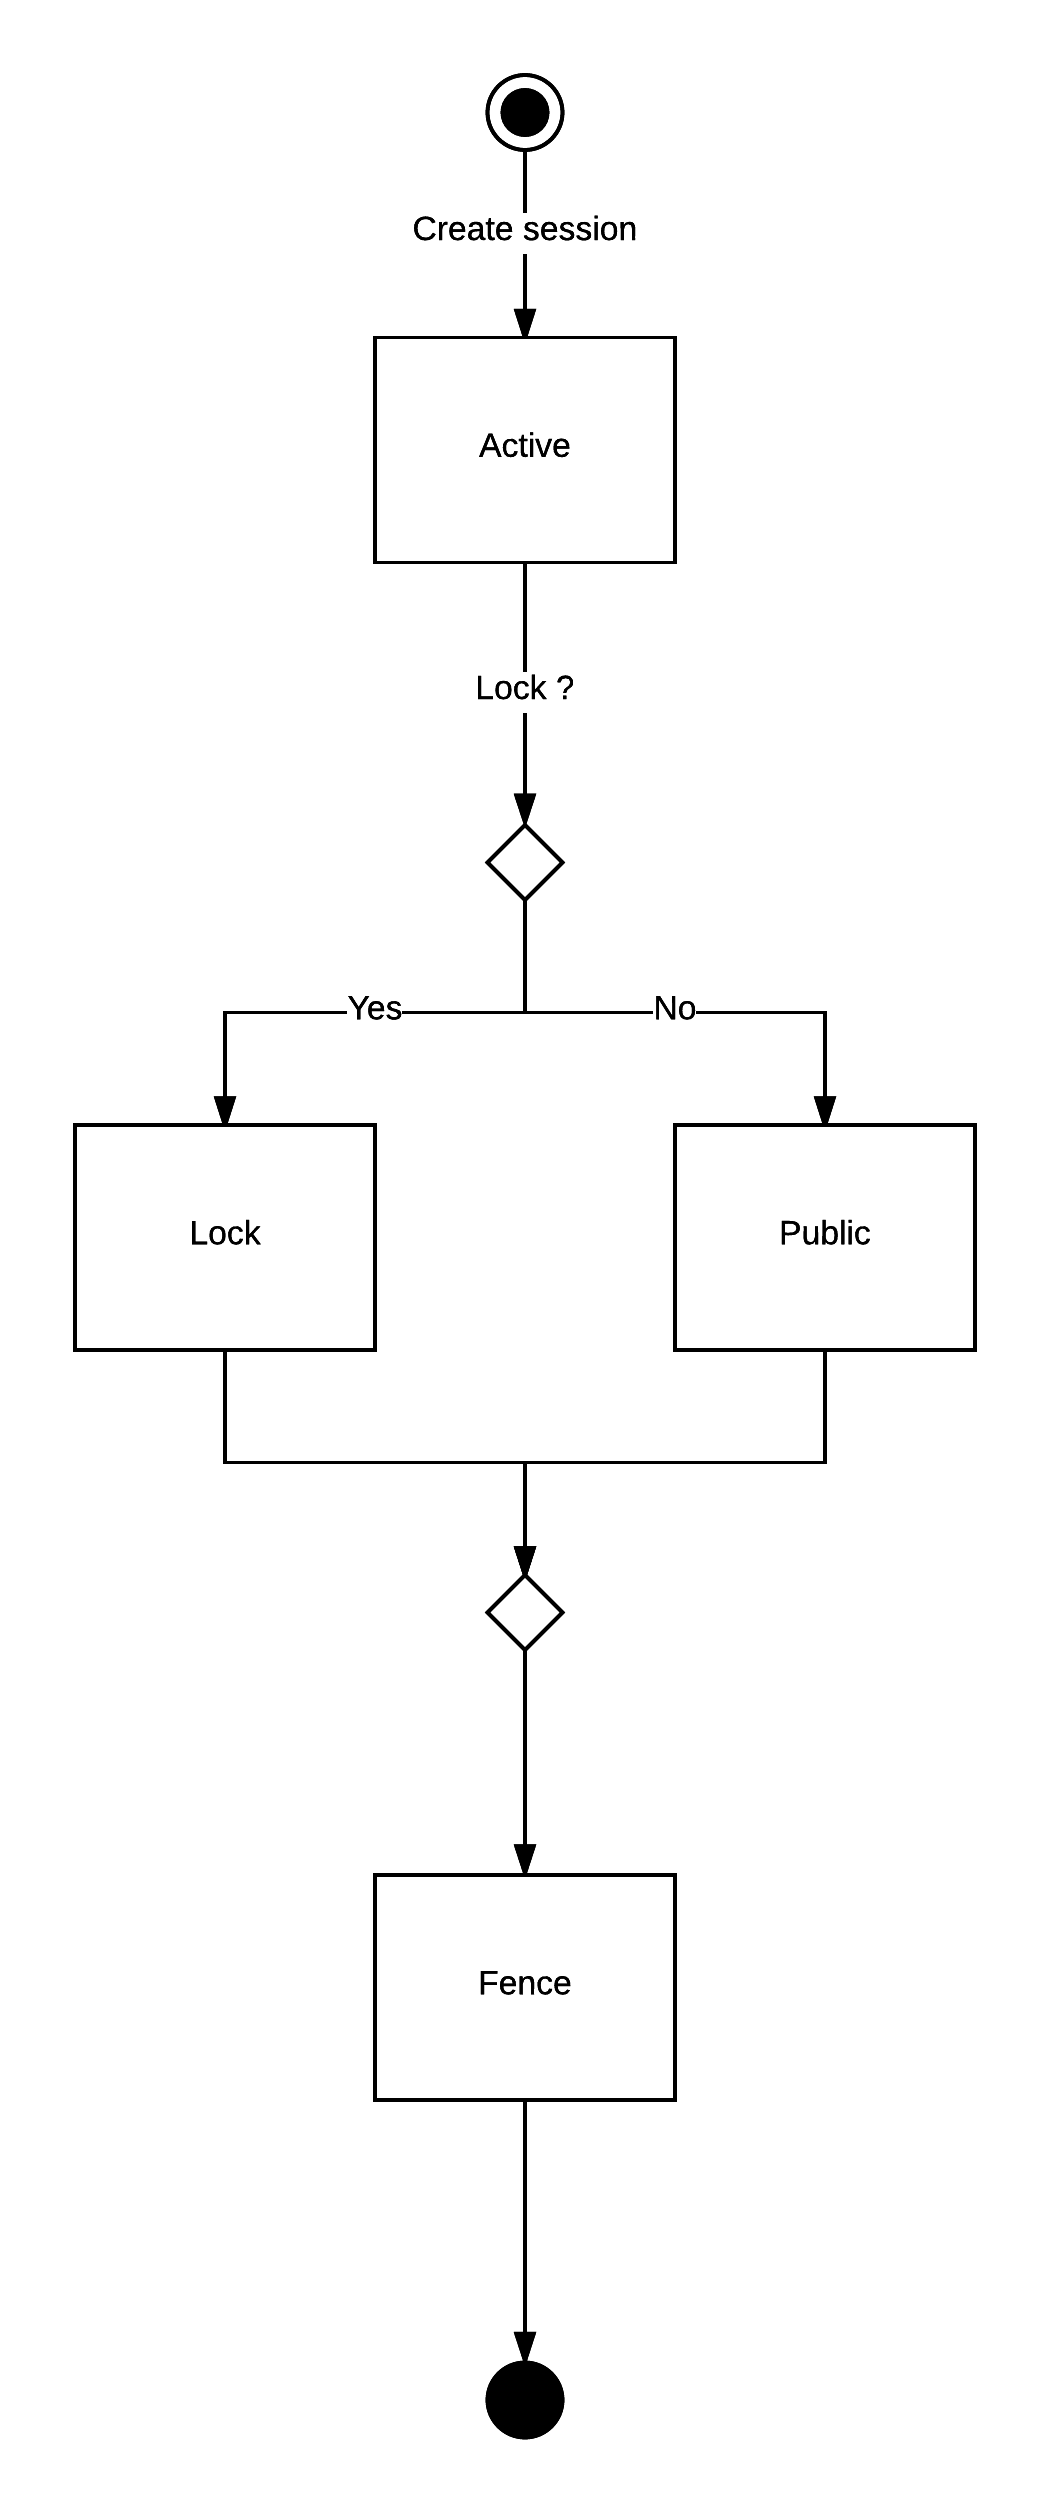
\includegraphics[scale=0.8]{Images/diagram/state_session_diagram.png}
\end{figure}

\end{document}       
